% Process:
% issues are added as \note{\emph{Name}: problem is that x!=y}
% when issues are solved, they are commented out.

% STATUS
% Knud: we should do two documents, one short and precise one describing the standard and a longer one for
% explaining the decision made and the design rationale.
% Renauld and Knud work on it from DERI side.

% next todos:

% TODO: I often used the syntax <pimo:<Name>> to describe elements of the ontology, they should later be hyperlinked to the description in the appendix. Linking these elements to the ontology should be done in a script.

% DONE:
% 20.06.2007 : Leo adds his latest status on the core questions and answers that PIMO should give, also explaining the ontology from the rdfs folder.
% LEO: check if all NAO has been used
% LEO: copy/paste mid/domain-level stuff from iSemantics Paper

% SOURCES FROM WHERE LEO COPY/PASTED - code will contain comments where this happened
% SauermannElstDengel2007 - the PIMO paper at ISemantics 2007
% SauermannDissertation - Leo's diss, the soon-ending project. There is an intended overlap between SauermannElstDengel2007 and the diss.

% History:
% 10.8.2007: Knud commits review, Leo works on arguments
% 20.06.2007: Leo and Knud skype and exchange plans.
% 29.06.2007: Leo has a first draft for review, this now reflects Leos view and the most important decisions made, Ludger and Sintek have to review to achieve a DFKI view.
% 12.09.2007: Leo and Knud Skype.
%             LEO: take agreed problem EQUIVALENCE, document it, move it to solved.

% INPUT AND INSPIRATION
% This document should use other RDF standards as input, these are well known documents:
% http://www.w3.org/TR/rdf-schema/ RDFS Primer
% http://www.w3.org/TR/swbp-skos-core-guide SKOS Core guide
% http://svn.nepomuk.semanticdesktop.org/repos/trunk/taskforce/TF-Ont/draft/NRL.html NRL spec (draft)


\documentclass[11pt]{nepomuk}
\usepackage{hyperref}		% turn on when latex is used (not miktec)
\usepackage{url} % LEO: urls \url{}
\usepackage{verbatim} % code and comment
\usepackage{longtable}
\usepackage{xspace}   % whitespace after a macro if no punctuation after the macro
\usepackage{microtype} % maybe fixes hyphenation in \texttt{pimo:Thing} sentences, see http://newsgroups.derkeiler.com/Archive/Comp/comp.text.tex/2007-08/msg01174.html
%\usepackage[htt]{hyphenat} 
\parindent0pt

\begin{document}
% explicit hyphenations
\hyphenation{RDF-Re-po-si-to-ry}
\hyphenation{name-space}
\hyphenation{So-cket-A-dap-ter}


% DEBUGGING HBOXES
%\overfullrule=5pt

% OUR chosen wording:
% Thing uppercase
% sub-property and sub-class instead of subproperty in prosa-text.

% even with goodwill and installing winfonts, 
% \emph does NOT work with tahoma.
% \fontfamily{tahoma}\selectfont 
%\def\note#1{\marginpar{\footnotesize#1}} % use this to show the notes in the document
\def\note#1{} % use this to hide the notes

\def\ie{\textit{i.\,e.},\ }
\def\eg{\textit{e.\,g.},\ }

\newcommand{\pimo}{\emph{PIMO}\xspace}
\newcommand{\pimos}{\emph{PIMO}s\xspace}
\newenvironment{definition}{}{}

%%%%%%%%%%%%%%%%%%%%%%%%%%%%%%%%%%%%%%%%%%%%%%%%%%%%%%%%%%%%%%%%%%%%%%%%%%%%%%%%
% TITLE PAGES 
%%%%%%%%%%%%%%%%%%%%%%%%%%%%%%%%%%%%%%%%%%%%%%%%%%%%%%%%%%%%%%%%%%%%%%%%%%%%%%%%
\thispagestyle{empty}

\pagenumbering{roman}

\hspace*{-4.5cm}
\begin{minipage}[p]{7cm}
\begin{large}
\textcolor{nepomuk@lightblue}{
\begin{tabular}{l}
Integrated Project \\
Priority 2.4.7 \\ 
Semantic based knowledge systems\\ 
\end{tabular}
}
\end{large}
\end{minipage}

\vspace{-2.8cm}


\begin{flushright}
	\includegraphics*[width=3.89cm]{images/InformationSocietyTechnologies}
\end{flushright}

\vspace{0.5cm}

\begin{flushright}
	
\includegraphics[width=12cm]{images/Nepomuk}
\end{flushright}


\vspace{1cm}


\textcolor{nepomuk@lightblue}{\rightline{\Huge{\bfseries \sffamily Personal Information Model (PIMO)}}} 
\textcolor{nepomuk@lightblue}{\rightline{\Huge{\bfseries \sffamily Ontology Guide}}} 

\vspace{0.3cm}

\textcolor{nepomuk@green}{\rightline{\huge NEPOMUK Recommendation v1.1}}

\vspace{0cm}

%\begin{figure}[h!]
\begin{flushright}
	
\includegraphics[width=9cm]{images/Bubbles}
\end{flushright}
%\end{figure}


\vspace*{-5.5cm}

\renewcommand{\arraystretch}{1.2}
\hspace*{-4.5cm}
\begin{minipage}[p]{11cm}
\begin{large}
\textcolor{nepomuk@red}{
\begin{tabular*}{8cm}{l@{\extracolsep{\fill}}l}
\multicolumn{2}{l}{\Large Version 1.1} \\
\multicolumn{2}{l}{\Large  02.02.2009} \\ 
\multicolumn{2}{l}{\Large  Dissemination level: PU} \\
\\ 
Nature & Report \\
%Due date & 31.05.2006  \\
Lead contractor	& DFKI\\ 
Start date of project	\qquad & 01.01.2006  \\ 
Duration & 36 months \\
\end{tabular*}
}
\end{large}
\end{minipage}

\clearpage
%%%%%%%%%%%%%%
% NEXT PAGES %
%%%%%%%%%%%%%%
\pagestyle{scrheadings}

\cohead{\small\textcolor{nepomuk@lightblue}{NEPOMUK}}
\rohead{\small\textcolor{nepomuk@lightblue}{02.09.2008}}
\lofoot{\small\textcolor{nepomuk@lightblue}{Task Force Ontologies}}
\cofoot{\small\textcolor{nepomuk@lightblue}{Version 1.0}}
\rofoot{\small\textcolor{nepomuk@lightblue}{\thepage}}

\newpage

\section*{Authors}
\hspace*{-2,5cm}\begin{minipage}[p]{14cm}
Leo Sauermann, DFKI \\
Ludger Van Elst, DFKI \\
Knud M\"oller, DERI\\
\end{minipage}


\vfill
\section*{Project Co-ordinator}
\hspace*{-2,5cm}\begin{minipage}[p]{14cm}
Dr. Ansgar Bernardi \\
German Research Center for Artificial Intelligence (DFKI) GmbH \\
Trippstadter Strasse 122 \\
D 67663 Kaiserslautern \\
Germany \\
Email: bernardi@dfki.uni-kl.de, phone: +49 631 205 3582, fax: +49 631 205 4910 \\
\end{minipage}


\section*{Partners}
\hspace*{-2,5cm}\begin{minipage}[p]{14cm}
DEUTSCHES FORSCHUNGSZENTRUM F. KUENSTLICHE INTELLIGENZ GMBH  \\
IBM IRELAND PRODUCT DISTRIBUTION LIMITED \\
SAP AG \\
HEWLETT PACKARD GALWAY LTD \\
THALES S.A. \\
PRC GROUP - THE MANAGEMENT HOUSE S.A. \\
EDGE-IT S.A.R.L \\
COGNIUM SYSTEMS S.A. \\
NATIONAL UNIVERSITY OF IRELAND, GALWAY \\
ECOLE POLYTECHNIQUE FEDERALE DE LAUSANNE \\
FORSCHUNGSZENTRUM INFORMATIK AN DER UNIVERSITAET KARLSRUHE \\
UNIVERSITAET HANNOVER \\
INSTITUTE OF COMMUNICATION AND COMPUTER SYSTEMS \\
KUNGLIGA TEKNISKA HOEGSKOLAN \\
UNIVERSITA DELLA SVIZZERA ITALIANA \\
IRION MANAGEMENT CONSULTING GMBH

\vspace{0.3cm}
\begin{footnotesize}
Copyright: NEPOMUK Consortium 2006\\
Copyright on template: Irion Management Consulting GmbH 2006
\end{footnotesize}
\end{minipage}

\clearpage


\section*{Versions}

\begin{footnotesize}
\begin{tabular}{|c|c|p{8cm}|}
\hline
\rowcolor{nepomuk@lightblue}\textcolor{white}{Version} &
                            \textcolor{white}{Date} &
                            \textcolor{white}{Reason} \\ \hline
0.1 & 01.06.2007 & a template of the document prepared by Antoni Mylka \\ \hline
0.9 & 12.08.2008 & Finished for review. \\ \hline
1.0 & 02.09.2008 & Reviewed and accepted. \\ \hline
1.1 & 02.02.2009 & Incorporating new handling of Tagging \\ \hline
\end{tabular}
\end{footnotesize}

\color{black}

\vfill
{\bf Explanations of abbreviations on front page}\\
\\
Nature \\
R: Report \\
P: Prototype \\
R/P: Report and Prototype \\
O: Other \\
 \\
Dissemination level \\
PU: Public \\
PP: Restricted to other FP6 participants \\
RE: Restricted to specified group \\
CO: Confidential, only for NEPOMUK partners \\

\newpage

%%%%%%%%%%%%%%%%%%%%%
% TABLE OF CONTENTS %
%%%%%%%%%%%%%%%%%%%%%
\setcounter{tocdepth}{2}
\tableofcontents
\cleardoublepage
\pagenumbering{arabic}

%%%%%%%%%%%%%%%%%%%%%%%%%
% BEGINNING OF SECTIONS %
%%%%%%%%%%%%%%%%%%%%%%%%%
\clearpage
\section{Abstract}
The PIMO Ontology can be used to express Personal Information Models of individuals. It is based on RDF and NRL, the NEPOMUK Representational Language and other Semantic Web ontologies. This document describes the principle elements of the language and how to use them.

\section{Status of this document}
This section describes the status of this document at the time of its publication. The form used for this status message and document is inspired by the W3C process. 

This document is an NEPOMUK recommendation produced by Leo Sauermann and Knud M\"oller as part of the task-force Ontologies in the NEPOMUK Project.
The document has been promoted from a draft form to this official form upon reviewing by the general NEPOMUK consortium. Subsequent versions of PIMO might mean that the specification documents of the later versions render this document obsolete, with respect to the version of PIMO in use, but not with respect to this version.

%\note{\emph{Knud}: Is PIMO really a language?}
%\note{\emph{Leo}: probably not, its an ontology}
This document and the PIMO ontology as such is a continuation and improvement of existing work. Other documents may supersede this document. 
Parts of this document will be published in other documents, such as scientific publications. This document is based on various other publications by the authors, and is a continuation of existing work. Some formulations from the RDFS primer and SKOS primer documents were reused.

Additional to this document, a FAQ is maintained in the public NEPOMUK 
wiki\footnote{\url{http://dev.nepomuk.semanticdesktop.org/wiki/PimoFaq}}.
\textbf{This document is accompanied by a RDFS/NRL ontology\footnote{\url{http://www.semanticdesktop.org/ontologies/2007/11/01/pimo\#}}, which should be downloaded (see Section~\ref{sec:downloadingpimo}) and read in parallel to learn more about PIMO.}

The key phrase ``\textbf{At Risk of Change}'' is used to mark parts of the recommendation
that are under discussion and change in future versions (can appear in footnotes).

The editors of this document value feedback from from the public and from the NEPOMUK consortium.
Typographic errors and change requests of the ontology can be reported using the NEPOMUK tracker\footnote{\url{https://dev.nepomuk.semanticdesktop.org/newticket}}, using the category \textbf{ontology-pimo}. General questions about using the ontology will be answered in the FAQ.
Subsequent versions of the ontology will include improvements gathered in this way.

We want to thank our reviewers for their feedback: Ansgar Bernardi, Siegfried Handschuh, P\"ar Lanner\"o, Enrico Minack, Gerald Reif, and Max V\"olkel.


\section{Introduction}
\label{sec:introduction}
\pimo is the abbreviation for the \emph{Personal Information Model} of a user. The PIMO-Ontology is both an RDF vocabulary\footnote{More precisely, PIMO is based on the NEPOMUK Representational Language (NRL), which extends the RDF model with a semantic model and support for named graphs and other features. However, for the sake of simplicity, we will use the term RDF throughout most of this document.} to express such a model and an upper ontology defining basic classes and properties to use.

Readers of this document should be familiar with the Resource Description Framework on the level described in the RDFS-Primer~\cite{rdfs} and the NRL specification\footnote{\url{http://www.semanticdesktop.org/ontologies/nrl/}}. 
The emphasized key words ``\textbf{must}'', ``\textbf{must not}'', ``\textbf{required}'', ``\textbf{shall}'', ``\textbf{shall not}'', ``\textbf{should}'', ``\textbf{should not}'', ``\textbf{recommended}'',  ``\textbf{may}'', and
``\textbf{optional}'' in this document are to be interpreted as described in
RFC 2119.

The scope of a PIMO is to model data that is within the attention of the user and needed for knowledge work or private use. The focus is on data that is accessed through a Semantic Desktop or other personalized Semantic Web applications. We call this the \textbf{Personal Knowledge Workspace}~\cite{HolzMausBernardiRostanin2005b} or \textbf{Personal Space of Information (PSI)}~\cite{pim2007},
embracing all data ``\emph{needed by an individual to
perform knowledge work}''. It is (1) independent from the way the user accesses the data, (2) independent from the source, format, and author of the data. 
The abbreviation \textbf{PSI} will be used.
\note{\emph{Knud}: This is a strange sentence. What does ``never part of computerized systems'' mean? Is ``Love'' such data?\\
\emph{Leo}: Added a sentence below about ``existing information''}
%Is Data that is never part of computerized systems is out of scope. 


Today, such data is typically stored in files, in Personal Information Management (PIM) or in groupware systems. A user has to cope with 
\note{\emph{Knud}: What is ERP?} different formats of data, such as text documents, contact information, e-mails, appointments, task lists, project plans, or an Enterprise Resource Planning (ERP) system. 
% replacement for the ``Love'' problem above:
Existing information that is already stored in information systems is in the scope of PIMO, but abstract concepts (such as ``Love'', ``Language'') can also be represented, if needed.

%Existing information is represented using the NEPOMUK Information Element (NIE) ontology framework~\footnote{\url{http://www.semanticdesktop.org/ontologies/nie/}}. It defines classes for  Information Elements, such as e-mails, documents, appointments, and contacts. 

%\note{\emph{Knud}: Why XML TMs? It's the model that matters, not the syntax, right?
%\emph{Leo}: Topic Maps has a different approach to modelling than RDF. Especially
%indirect identification using identifiers is clearly specified in TM, but not in RDF. Moved the reference to TM a bit lower and adding a note to identity} 

%Similar to SKOS,
PIMO is based on the idea that users have a \emph{mental model} to categorize their environment. 
It represents the user itself and the fact that he has a \emph{Personal Information Model}, this is described in Section~\ref{sec:pimo-user}. 
Building a PIMO for the imaginary user \textit{Claudia Stern} is the guiding example for this document. 
Each concept in the environment of the user is represented as \emph{Thing} in the model,
and mapped to documents and other entities that mention the concept (see Section~\ref{sec:thing}).
Things can be described via their relations to other Things or by literal RDF properties,
the key properties are defined in Section~\ref{sec:describingthings} and directions given 
how to use them. 
An important question is the class of a Thing; the semantics of classes and top level classes are presented in Sections~\ref{sec:classofthing}-\ref{sec:pimoUpperClasses}.
To match and align similar concepts, existing identification systems are reused and integrated (Section ~\ref{sec:identification}).

PIMO is similar to SKOS or Topic Maps (TM)~\cite{iso13250second} in its goal of providing an easy way of modelling, but different in the way concepts are modeled. RDFS classes and sub-class relations (which are used in NRL) are used to represent the classes of Things, individuals are represented using typed RDF resources. From TM, the idea of indirect identification is taken up.
%, in this regard PIMO is similar to OWL. 
%\note{\emph{Knud}: this sounds very weird. PIMO is similar to OWL because it uses RDFS class and instances are RDF resource? Then PIMO is first and foremost similar to RDFS!
%\emph{Leo}: Removed the reference to OWL, not needed. Reference to RDFS is implicit.} 

%\note{\emph{Knud}: really? Each element is a pimo:Thing?
%\emph{Leo}: Thing and subclasses, but thats the key idea, we have to discuss and agree on this.} 
%\note{\emph{Knud}: of course sameAs is directed! Every arc in an RDF graph is directed! Also, directedness and whether or not resources form a graph are not contradictions, so why do you say ``rather''?
%\emph{Leo} owl:sameAs is symmetric, so the direction is not known, the inverse of sameAs is sameAs. In pimo, directed relations are used, with the Thing as subject and the resource as object}
PIMO is different from OWL, where \texttt{sameAs} relations are symmetric equivalence relations forming a fully connected graph amongst identical resources. 
In PIMO, Things are connected to their equivalent resources using directed relations.

The design rationale %(see Section~\ref{sec:designrationale}) 
is to keep the PIMO ontology as minimal as possible, and also the data needed to create a PIMO for a user as minimal as possible. Inside one PIMO of a user, duplication is avoided. 
PIMO builds on Semantic Desktop ontologies (NRL, NIE, NAO) and guidelines are provided how to reuse other existing RDFS ontologies (Section~\ref{sec:integratingontologies}) and import data expressed in these ontologies.
After importing, rules are used to integrate facts (see Section~\ref{sec:integratingfacts}). 
% this is a typical ``summary'' sentence, but in a standards document, there are usually no ``summary'' sections, so it remains here. REALLY, the RDFS primer has no summary nor has the SKOS primer. live with it.
% BTW: Leo invested four fucking years into this, so the reader HAS the 20 seconds time to read this.

Only by addressing all key issues --- precise representation, easy adoption, easy to understand by users, extensibility, interoperability, reuse of existing ontologies, data integration --- PIMO provides a framework for creating personal information management applications and ontologies.

\subsection{Downloading PIMO}
\label{sec:downloadingpimo}
The RDF descriptions of the ontology can be retrieved from its namespace using content negotiation:
{\small
\begin{verbatim}
Namespace:
http://www.semanticdesktop.org/ontologies/2007/11/01/pimo#
\end{verbatim}
}

Different serializations are available:
\begin{itemize}
	\item XML/RDFS Serialization: PIMO (Data Graph Only)\\
	 {\small\url{http://www.semanticdesktop.org/ontologies/2007/11/01/pimo/pimo_data.rdfs}}
	\item XML/RDFS Serialization: PIMO (Metadata Graph Only)\\
	 {\small\url{http://www.semanticdesktop.org/ontologies/2007/11/01/pimo/pimo_metadata.rdfs}}
	\item TriG Serialization: PIMO (Graph Set)\\
	 {\small\url{http://www.semanticdesktop.org/ontologies/2007/11/01/pimo/pimo.trig}}
\end{itemize}    

\section{PIMO integrates with key ontologies}
The PIMO framework does not stand alone but is part of a set of 
carefully designed and integrated ontologies for the Semantic Desktop 
which were developed in parallel to provide an integrated framework.
In Figure~\ref{fig:roadmap} an overview is given.

\begin{figure}[htb]
	\centering
		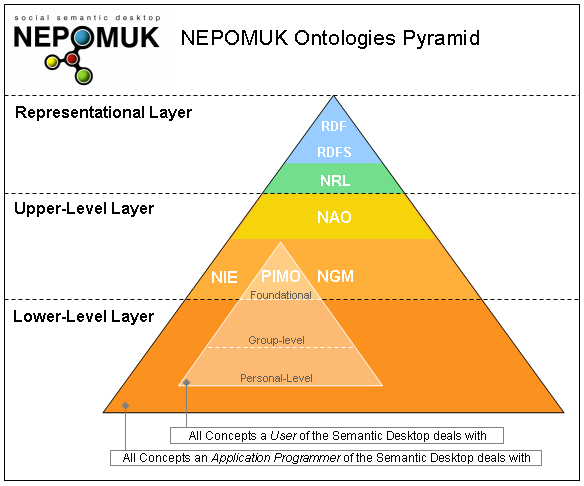
\includegraphics[width=1.00\textwidth]{images/roadmap.png}
	\caption{Integrated Ontologies}
	\label{fig:roadmap}
\end{figure}

The NEPOMUK Representational Language \textbf{NRL ontology}\footnote{\url{http://www.semanticdesktop.org/ontologies/nrl/}} builds the representational layer and the semantic
metadata axioms used to express PIMO. 
NRL is a meta-language comparable to OWL or RDF/S. 
The key characteristics of NRL are (on top of RDF/S) support for named graphs
in semantic statements, a notation for contextualized inference and semantics, 
and a selection of semantic relations (inverse, transitive, reflexive).

The NEPOMUK Information Element \textbf{NIE ontology}\footnote{\url{http://www.semanticdesktop.org/ontologies/nie/}} describes desktop elements such as address book entries, documents,
e-mails, appointments, pictures, and multimedia files.
The ontology discriminates between the representation (binary files)
and the information stored therein. 
PIMO reuses the classes of NIE and suggests how to integrate
and annotate vast personal spaces of information (PSI) expressed in NIE.

Annotations and tagging are represented in the NEPOMUK Annotation \textbf{NAO ontology}.
It represents change-dates, author, and other key metadata of documents.
NIE and PIMO both extend NAO. A part of NAO is the NEPOMUK Graph Metadata \textbf{NGM ontology} to annotate named graphs.

The PIMO ontology crosses two of the layers in the ontology pyramid, data related to PIMO can be divided into three smaller layers (also visible in Figure\ref{fig:roadmap}):
\begin{itemize}
	\item \emph{Foundational PIMO}: The PIMO ontology as such, as defined in this specification and accompanying NRL serialization. This includes the classes and properties of \emph{PIMO-upper} (see Section \ref{sec:pimoupper}), which work on the \emph{Upper-Level Layer} of NEPOMUK and everything else defined in the PIMO vocabulary. PIMO-upper is the same for every Semantic Desktop user and is valid in a global context.
	\item \emph{Group-level PIMO}: Domain ontologies that are shared within a group. They can be imported by users. A description is given in Section~\ref{sec:pimomid}.
	\item \emph{Personal-level PIMO}: The classes, properties, and Things created by an individual user. Also called \emph{user-PIMO}, this layer includes the data that is only relevant in the context of one individual.
\end{itemize}

\section{Examples}
\label{sec:examples}
A scenario is used to explain the ontology elements. A fictional persona, Claudia Stern, is our example user. She is working for EX-Ample Inc., a fictional company producing ``\textbf{Ex}treme Guitar \textbf{Ampl}ifi\textbf{e}rs'', and her current task is to organize a business trip to a meeting with guitarists and bass players in Belfast.

% taken from RDFS primer
For convenience and readability, this specification uses an abbreviated form to represent URI-References. A name of the form \texttt{prefix:suffix} should be interpreted as a URI-Reference consisting of the URI-Reference associated with the prefix concatenated with the suffix.

RDF graphs are written in N3/Turtle syntax. Examples serialized as RDF appear in this typesetting:
%\note{\emph{Knud}: I find the statement (Claudia user Claudia) very confusing. What's that supposed to mean? \emph{Leo}: that was garbage, we had it in the ontology before as an alternative to isDefinedBy.}
{\small
\begin{verbatim}
claudia:Claudia a pimo:Person;
 pimo:isDefinedBy claudia:PIMO;
 nco:hasEmailAddress <mailto:claudia@example.com> .
\end{verbatim}
}

\subsection{PIMO ontology and namespaces}
The ontology described in this document has this namespace:

{\small
\begin{verbatim}
Namespace:
http://www.semanticdesktop.org/ontologies/2007/11/01/pimo#
\end{verbatim}
}

During the lifetime of the NEPOMUK project (until Dec 2008), the PIMO ontology
and the according documentation may change, but the namespace will not change.
The namespace stays fixed to keep the necessary changes
of software implementations at a minimal level.
We have adopted this practice from other projects, which have applied it successfully. Examples are the W3C's  XSD datatypes (the recommendation changed in 2007, the namespace did not) or the FOAF project.

Throughout this document these ontologies and namespaces are used, also indicating their respective versions PIMO is building on:
{\small
\begin{verbatim}
@prefix rdf:  <http://www.w3.org/1999/02/22-rdf-syntax-ns#>.
@prefix rdfs: <http://www.w3.org/2000/01/rdf-schema#>.
@prefix nrl:  <http://www.semanticdesktop.org/ontologies/2007/08/15/nrl#>.
@prefix nao:  <http://www.semanticdesktop.org/ontologies/2007/08/15/nao#>.
@prefix pimo: <http://www.semanticdesktop.org/ontologies/2007/11/01/pimo#>.
@prefix ncal: <http://ont.semanticdesktop.org/ontologies/2007/04/02/ncal#>.
@prefix nco:  <http://ont.semanticdesktop.org/ontologies/2007/03/22/nco#>.
@prefix nfo:  <http://ont.semanticdesktop.org/ontologies/2007/03/22/nfo#>.
@prefix nie:  <http://www.semanticdesktop.org/ontologies/2007/01/19/nie#>.
@prefix nmo:  <http://www.semanticdesktop.org/ontologies/2007/03/22/nmo#>.

@prefix claudia: <http://www.example.com/people/claudia#> .
\end{verbatim}
}

\section{Creating Personal Information Models}
\label{sec:creatingPIMOs}
In this section, all key elements of the ontology are presented.
The order used reflects the steps a knowledge engineer will have to take to implement this recommendation.

\subsection{The User and their Individual PIMO}
\label{sec:pimo-user}
As a prerequisite to create a PIMO and Things inside the PIMO, each user needs a \emph{personal namespace}. The namespace is used as a prefix for all URIs minted for the user. Often these are namespaces using the HTTP URI scheme, but any RDF namespace can be used. The example namespace used in this document is \texttt{http://www.example.com/people/claudia\#} and is abbreviated with ``\texttt{claudia:}''.

\note{\emph{Knud}: In general, I would write all ontology elements in a different font. E.g., \texttt{pimo:Person}
\emph{Leo}: actually, I would like to write a script that, once this is converted
to HTML, replaces all ``pimo:NAME'' with HTML links to the ontology definition 
within the namespace.
\emph{Knud, 28/12:} unfortunately, there isn't always a namespace given. For now, I changed all ontology elements to monospaced font}

Users are represented as instances of the class \texttt{pimo:Person}. For each instance, a new URI is generated and a few key facts are represented to identify the user.
After the user has been instantiated, details such as email addresses are added by using terms from the NEPOMUK contact ontology, NCO. 
%\note{Knud: What do you mean by ``as the second object''? \emph{Leo}: fixed this, its a new resource.} 
In NCO, contact information connected to people is modeled as a complex resource, not as a simple literal:
%For the sake of simplicity, we used the URL \texttt{mailto:claudia@example.com} as identifier for this nco:EmailAddress resource.
{\small
\begin{verbatim}
claudia:Claudia a pimo:Person;
 rdfs:label "Claudia Stern";
 nco:hasEmailAddress mailto:claudia@example.com.

mailto:claudia@example.com a nco:EmailAddress;
 nco:contactMediumComment "work";
 nco:emailAddress "claudia@example.com".
\end{verbatim}
}

The second entity that needs to be represented is the \emph{Personal Information Model of the User}. It is connected to the user via the \texttt{pimo:creator} relation, and the user's namespace is added.
For Claudia this is:

{\small
\begin{verbatim}
claudia:PIMO a pimo:PersonalInformationModel;
  pimo:creator claudia:Claudia;
  nao:hasDefaultNamespace "http://www.example.com/people/claudia#";
  nao:hasDefaultNamespaceAbbreviation "claudia".
\end{verbatim}
}

\texttt{pimo:PersonalInformationModel} is a sub-class of \texttt{nrl:Ontology}, allowing more metadata to be added using NRL compliant standards. More about NRL metadata is described in Section~\ref{sec:nrlgraphs}. 
We further call a this instance of \texttt{pimo:PersonalInformationModel} of an individual a \emph{user-PIMO}. Claudia's user-PIMO is \texttt{claudia:PIMO}. As an abbreviation, it is also correct to write  ``Claudia's PIMO'' instead of ``Claudia's user-PIMO''.
\note{\emph{Knud, 28/12:} I'm confused by this term PIMO-user. It sounds as if it meant ``The user of the PIMO'', but it actually means ``The PIMO of the user'' --- correct? That's potentially confusing.} 
\note{\emph{Leo, 8/1:} reduce to ``user's PIMO'' and ``Claudia's PIMO''?}

\subsection{Things}
\label{sec:thing}
The PIMO ontology defines the basic class \texttt{Thing} for mental concepts. Every information element encountered in knowledge work by a user is represented as a Thing.
\note{\emph{Knud, 28/12:} Thing is inconsistently spelled with lower- and upper-case throughout the document.}
A Thing is a unique representation of an entity of the real world within one user-PIMO. On the PSI of a user, a real world entity can be represented in multiple data sources. For example, the person ``Dirk Hagemann'' may be author of an e-mail, described in an address book entry, and stored in a accounting tool, all part of the workspace of ``Claudia''. 
One instance of \texttt{pimo:Person} is created as unique \texttt{Thing} linking to these multiple representations, such as shown in Figure~\ref{fig:thing_vs_resource}.
\note{\emph{Knud, 28/12:} Yes, this is a Thing, but it is also a pimo:Person? Potentially confusing. \emph{Leo, 8/1:} changed the wording to speak of a Person}

\begin{figure}[htbp]
	\centering
		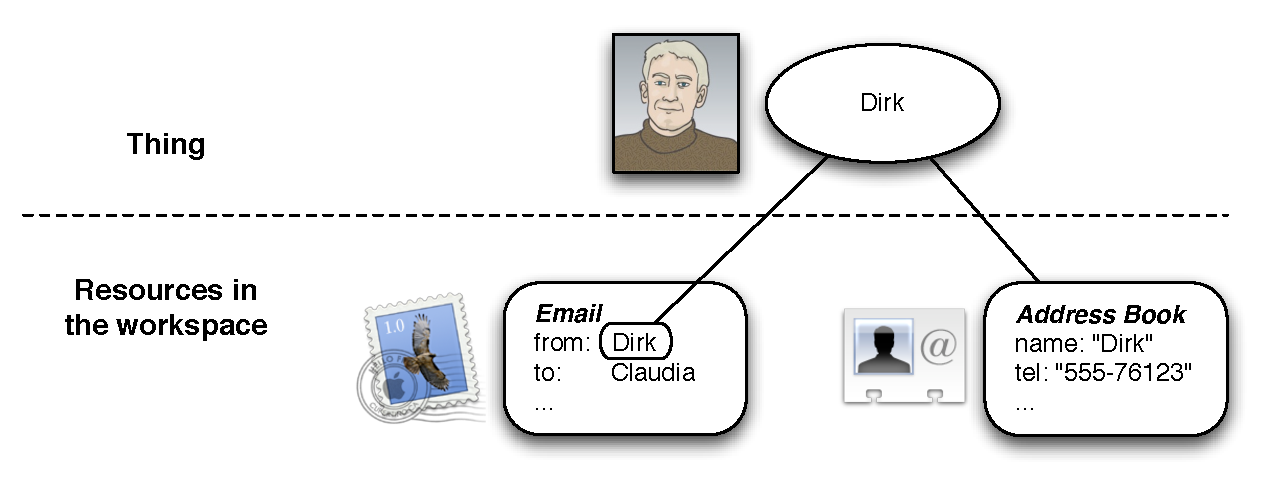
\includegraphics[width=1.00\textwidth]{images/thing_vs_resource}
	\caption{Thing and Resources}
	\label{fig:thing_vs_resource}
\end{figure}

An application handling a resource in the workspace can be aware that there may be a Thing representing the resource. For example, Claudia's e-mail client may examine the sender of an e-mail (Dirk) and search for the \texttt{pimo:Thing} that represents Dirk uniquely. Once the right Thing is found by the application, more information about Dirk can be discovered.

This principle includes all elements (\texttt{nie:InformationElement} and other RDF resources) in the user's \emph{Personal Space of Information (PSI)}. 
For each information element, a Thing in the user's PIMO must be created. 
The information element exists independent of the user, the same element can
be stored in multiple folders or data sources on one desktop, and also on other desktops and on the web. 
A Thing is the personalized view of \emph{one user} on this information element, independent of representation or storage location.

To be adequate, a PIMO of a user should contain all nameable entities known to the user,
but to be efficient, this representation should be restricted to the minimal data needed.
%Leo 29.7.2008: this is also explained later
% Identification is part of this minimal data, and \texttt{nao:identifier} provides the property for it.

\subsection{Connecting Things to the User's PIMO}
\label{sub:connectingThingsToPimo}
In a scenario of multiple connected semantic desktops, it will frequently occur that users import data from each other's desktop onto their own desktop.
It is therefore important to know which resources (primarily Things, but also Classes and Properties) were created by which user and originate from which PIMO. For this, the property \texttt{pimo:isDefinedBy} is used.

Continuing the example above, this property connects the Person to the PIMO in which it is defined.  This is mandatory for every defined Thing and allows applications to identify which elements are part of a user-PIMO and which are not\footnote{We intentionally did not only rely on NRL graphs to model the relation between the model and instances defined by it. A graph can only contain \emph{statements}, 
about, but not \emph{resources} as such.
To model that a resource is part of a PIMO, the \texttt{pimo:isDefinedBy} relation is a clear representation.
Additionally, named graphs can be used to declare what \emph{statements} are declared in a PIMO, see~\ref{sec:nrlgraphs}}.

{\small
\begin{verbatim}
claudia:Claudia pimo:isDefinedBy claudia:PIMO.
\end{verbatim}
}

An \texttt{isDefinedBy} property is also defined in RDFS, where resources can be connected to their defining ontologies, and is also discussed in the light of the OWL standard\footnote{\url{http://www.w3.org/2007/OWL/wiki/Syntax\#Declarations_and_Structural_Consistency}}. 
The semantics of \texttt{isDefinedBy} in PIMO is based on these, with the extension that we define it as a required property.

\subsection{Identification of Things}
\label{sec:identification}
A Thing \textbf{must} have an URI and \textbf{should} be described with properties that identify it. 
Identifiers allow to analyse information elements and find occurrences of the Thing.
For example, the person ``Dirk Hagemann'' is represented once as an instance of the class \texttt{pimo:Person} and identified using his e-mail address. 
The RDF descriptions of emails and documents can then be analysed to find resources that represent the same entity via this identifier. 
{\small
\begin{verbatim}
# The canonical Dirk
claudia:DirkHagemann a pimo:Person;
 pimo:isDefinedBy claudia:PIMO;
 nco:hasEmailAddress <mailto:dirk@example.com>.

# An e-mail in which Dirk #2 occurs
<imap://claudia@example.com/INBOX/1> a nmo:Mail;
 nmo:from <imap://claudia@example.com/INBOX/1#from>.

# Dirk #2, the email sender
<imap://claudia@example.com/INBOX/1#from> a nco:Contact;
 nco:hasEmailAddress <mailto:dirk@example.com>.
<mailto:dirk@example.com> a nmo:EmailAddress;
 nco:emailAddress "dirk@example.com".
 
# Dirk #3, as address book contact
<file://home/claudia/dirk.vcf#dirk> a nco:PersonContact;
 nco:nameFamily "Hagemann";
 nco:nameGiven "Dirk";
 nco:hasEmailAddress <mailto:dirk@example.com>;
 nco:photo <http://www.example.com/people/dirk/photo.jpg>.
 
\end{verbatim}
}

In this example, we see that the Person Dirk appears three times in this knowledge workspace. First, in the form of an instance of \texttt{pimo:Person}, as the canonical Dirk. Second, as sender of an e-mail and third as entry in an address book. Only one instance is the \texttt{pimo:Thing} representation of Dirk: \texttt{claudia:DirkHagemann}. The others are information elements representing the same entity.

\begin{figure}[htb]
	\centering
		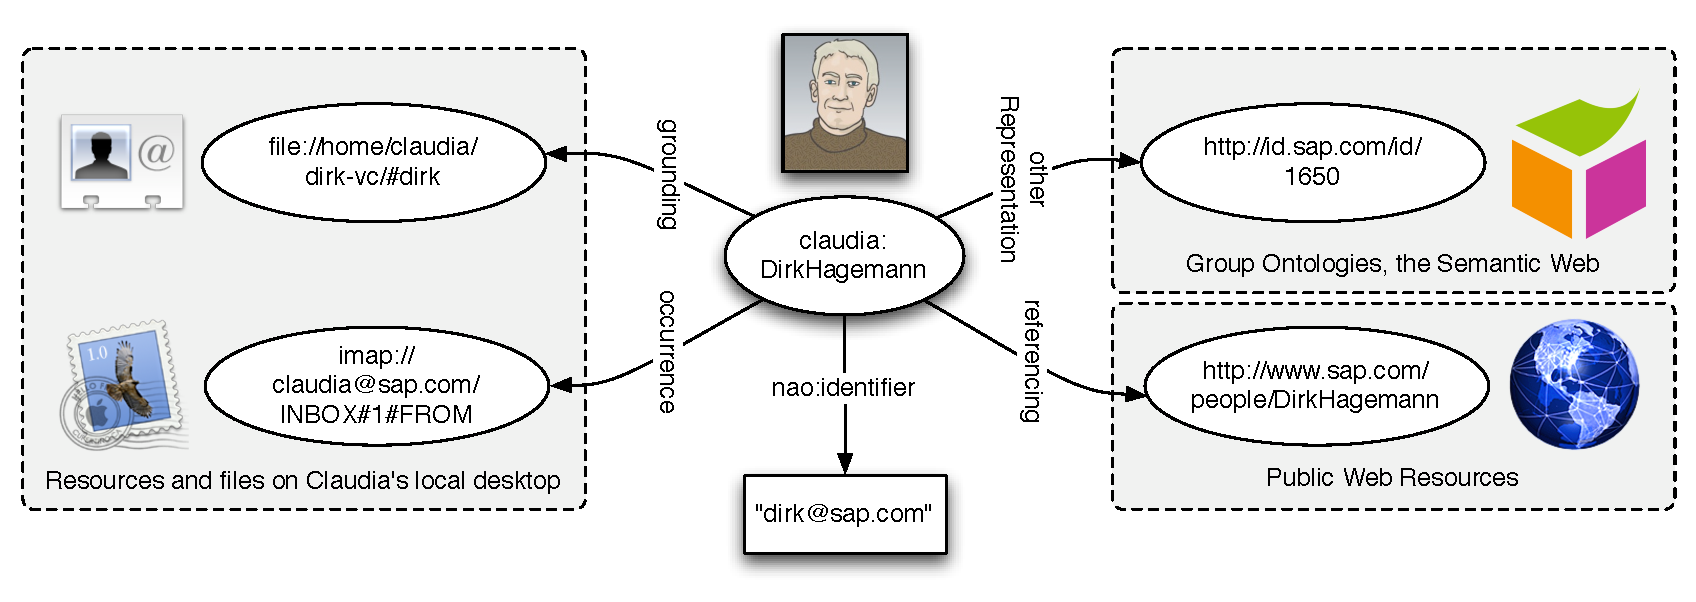
\includegraphics[width=1.00\textwidth]{images/identification}
	\caption{Different Identification Mechanisms}
	\label{fig:identification}
\end{figure}


%\note{\emph{Knud}: can one ``use'' an assumption? Leo: rephrased to ``is based on''}
To work effectively, PIMO is based on the \emph{Unique Name Assumption} (UNA). 
The UNA is a rule that declares two RDF resources with different URIs as different individuals. 
This is common in desktop applications (for example files with different names are different) and intuitive to grasp for users. But it is different from the OWL ontology language
%\note{\emph{Knud}: is OWL a system? Leo: its an ontology language}
where duplicate entries are common and the UNA is not enforced. 
PIMO is designed for personal systems, where an application has access to the complete model and can avoid duplicates before creating them.

To enforce the UNA, duplicate Things \textbf{must} be avoided. 
The crucial moment to do this is before creating a new Thing.
Things can either be created by the user manually or automatically by analysing existing native resources. In any case, before creating a new Thing, all existing Things have to be examined if a Thing with a same name or same identifying properties already exists. 
If an existing Thing is found, it \textbf{must} be reused. 
Immediately after creating a new Thing, identifying properties should be set to distinguish the Thing and avoid duplication. 
% fix to https://dev.nepomuk.semanticdesktop.org/ticket/498
Section \ref{sec:creatingthingalgorithm} further describes the complete process of creating things.

In the next paragraphs, essential identifying properties are described, an overview is given in Figure~\ref{fig:identification}.

\textbf{The primary identifier of a Thing is it's URI}. New URIs for Things \textbf{must} be generated using the namespace of the user as prefix and then a unique local name. 
Although the local name can be entirely a random string, we recommend to include the label in the URI for readability. When minting a new URI that clashes with an existing URI, a random element can be added to the new URI. A URI for Claudia Stern is:
\begin{verbatim}
claudia:Claudia
\end{verbatim}

\paragraph{NAO-Identifiers} Existing identification schemes based on NAO should be reused for this purpose by representing them with 
%\note{Knud: you say pimo:identifier here and nao:identifier in the example below. Which one is it?\emph{Leo}: its nao:identifier (28.8.2007).} 
\texttt{nao:identifier} and its sub-properties. 
If an identifier is found as meta-data of a native resource (usually an \texttt{nie:InformationElement}), the identifier \textbf{must} be copied to the Thing.
This allows others to match and identify the correct Thing when encountering the next information element.
Example identifiers are \texttt{nmo:messageId} for e-mails, \texttt{ncal:uid} for appointments, or \texttt{nexif:imageUniqueID} for images. 
Instead of using the plain \texttt{nao:identifier} property, these specific properties should be used or new sub-properties of \texttt{nao:identifier} created
\footnote{I.e. if you want to represent ISBN numbers and there is no property for them, create a new sub-property \texttt{isbn} of \texttt{nao:identifier}.}.
In this document, we assume that e-mail addresses can be used to identify persons.

\note{\emph{Leo}: this example is not good, as e-mail addresses are modeled 
differently in NCO. How else can we identify a person? \emph{Knud, 28/12:} I think we can't... :P}
\begin{verbatim}
# Copy all identifiers you can find about the Thing.
claudia:DirkHagemann a pimo:Person;
 nao:identifier "dirk@example.com".
\end{verbatim}

Identifiers consisting of multiple RDF statements cannot be captured using \texttt{nao:identifier}.
They are comparable to a primary key in a relational database consisting of multiple
columns. These \textbf{multi-key identifiers} \textbf{must} be merged into one \texttt{nao:identifier}.

\paragraph{Grounding Occurrence} The relation \texttt{pimo:groundingOccurrence} is used to link a Thing to an \texttt{nie:InformationElement} that has this Thing as primary topic. For example, the grounding for a person could be the entry in the address book describing the person. On the other hand, an e-mail with this person as the sender or recipient would normally not be a grounding occurrence. A Thing represents the mental concept, the \texttt{pimo:groundingOccurrence} links to existing Information Elements that are handled by existing applications. This is a key for reusing the features of these applications. 
The grounding occurrence can change, for instance if a file was moved and the URI of the Information Element changed, the grounding occurrence relation needs to be changed. 
A similar case happens when a file is uploaded to a shared workspace and not kept locally any more --- all annotations of the Thing stay the same (the URI of the Thing does not change), the Information Element changes.
Multiple values are allowed, this reflects the fact that the same Thing can be represented in multiple applications, and dependent on the work context, the user may want to open a different application. 
{\small
\begin{verbatim}
# Link to Dirk #3 from example above.
claudia:DirkHagemann a pimo:Person;
 pimo:groundingOccurrence <file://home/claudia/dirk.vcf#dirk>.
\end{verbatim}
}
\paragraph{Occurrence} The relation \texttt{pimo:occurrence} connects a \texttt{pimo:Thing} with a resource representing the same real world entity.
Facts about the occurrence are then also valid for the connected Thing. 
For example, if the person Dirk appears as sender of an e-mail, then the resource identifying the sender is an \emph{occurrence} of Dirk. 
Based on the occurrence relation, Dirk (the unique \texttt{pimo:Person}) is the sender of the given e-mail.
Occurrence relations are to be used on resources \emph{representing} the same entity in a different context, but not on resources \emph{mentioning} the entity. For example, it is not valid to say that an e-mail is an occurrence of a person, only the sender or recipient can be occurrences of a person.

%Not the e-mail as such is the occurrence, but the sender within. 
\note{\emph{Knud, 28/12:} Why is the e-mail as such not the occurrence? This should be explained, or not mentioned at all. 
Leo: done, removed sentence, replaced with longer explanation.}
Occurrences of a Thing can be found by searching for entities with the same identifying properties.

{\small
\begin{verbatim}
# Link to Dirk #2 from example above, 
# he occurs as sender of an e-mail
claudia:DirkHagemann a pimo:Person;
 pimo:occurrence <imap://claudia@example.com/INBOX/1#from>.
\end{verbatim}
}

Besides identification, both the \texttt{pimo:groundingOccurrence} and the \texttt{pimo:occurrence} relation have 
implications on data integration and affect semantic meaning of a Thing. 
This will be described later in Section \ref{sec:pimoVSnie}.

\paragraph{Referencing Occurrence} 
%\note{Maybe rename to indicatingOccurrence, closer to Topic Maps? Leo: I don't care, leave it as is.}
\label{par:referencingOccurrence}
A Referencing Occurrence is an indirect approach to identification. 
Annotating a Thing with an information element as \emph{referencing occurrence} states that the information element contains a description of the Thing.
Its primary topic must be the Thing.
The Thing is indirectly identified by the element, when two Things in different models share the same information element as referencing occurrence, they may be equal and could be matched. 
The following description is an adaption of XTM's subject indicators~\cite{XTM,Rath2003}.
The referencing occurrence is a kind of proxy for the Thing. Examples of referencing occurrences are:

{\small
\begin{verbatim}
claudia:DirkHagemann a pimo:Person;
 pimo:referencingOccurrence <http://www.example.com/people/DirkHagemann>.
 
claudia:ExampleInc a pimo:Organization;
 pimo:referencingOccurrence <http://www.example.com/>;
 pimo:referencingOccurrence <http://en.wikipedia.org/wiki/Example.com>.
\end{verbatim}
}

It should contain a human readable documentation describing the concept. The resource could be a document, ontology, video, audio, anything able to describe to a human what the concept is about. The resource is a reference to the concept of the Thing. 
A good example for a referencing occurrence is a wikipedia article.

A referencing occurrence describes the concept with the purpose of being widely used by ontologies. Consequently, it is important that the document describes exactly what concept it is about and what not. Even if the author works as accurately as possible, different people will never interpret a referencing occurrence 100\% the same way. However, the concept of referencing occurrences is worth using it, because it allows a shallow match of heterogenous information models, and because there is finally no alternative to it. 

\textbf{It is recommended to use wikipedia URIs as objects of referencing occurrences.} In contrast, URIs minted by \emph{DBPedia}\footnote{DBPedia is a Semantic Web representation of wikipedia and provides URIs for concepts, whereas wikipedia provides URIs for documents describing concepts. An example DBPedia URI is: \url{http://dbpedia.org/page/Berlin}} \textbf{must} be related using the \texttt{pimo:hasOtherRepresentation} relation.

\paragraph{Other Representation} 
\label{par:otherRepresentation}
The \texttt{pimo:hasOtherRepresentation} relation is used to connect \texttt{pimo:Things} with other representations of the same Thing in other Semantic Web ontologies. 
This can be the case with shared ontologies, such as company white page systems or Semantic Social Networking websites. 

The knowledge modeled should be compatible with the ontologies used by the user. An example for such other representation is\footnote{Using the URI scheme of the ECS University in our example domain. \url{http://id.ecs.soton.ac.uk/docs/}}:
\begin{verbatim}
claudia:DirkHagemann a pimo:Person;
 pimo:hasOtherRepresentation <http://id.example.com/person/1650>.
\end{verbatim}

Another example would be the city of Belfast where Claudia wants to travel to,
linked to the DBPedia entry about it:
\begin{verbatim}
claudia:Belfast a pimo:City, pimo:Tag;
  pimo:isDefinedBy claudia:PIMO;
  pimo:tagLabel "Belfast";
  pimo:hasOtherRepresentation <http://dbpedia.org/resource/Belfast>;
  geo:lat "54.5833333";
  geo:long "-5.9333333".
\end{verbatim}
The relation can be used both to identify Things by their other representations,
and to fetch more data.
In this example, the latitude and longitude are actually superfluous data,
as they can be retrieved from the other representation
in DBPedia.
Assuming Dirk also represents Belfast in his PIMO, but independent from Claudia,
but linking to the same DBPedia entry, algorithmically matching their different representations is straightforward.

\paragraph{Other Conceptualization}
To map user-generated classes to classes defined in other ontologies, the 
\texttt{pimo:hasOtherConceptualization} relation connects classes defined in a user's PIMO
with classes defined in domain ontologies. 
Classes defined in domain ontologies should be sub-classes of PIMO-upper classes, see Section \ref{sec:integratingontologies}. 

Implementations can use the \texttt{pimo:hasOtherConceptualization} to allow the user and algorithms
to map user--specific classes to classes defined in other ontologies,
without implying that there is a sub-class relationship.

\subsection{A Complete Example} 
A complete example for all different identification properties 
can now be built from the above annotations.

For Claudia, her co-worker Dirk Hagemann is identified and linked to occurrences like this:

{\small
\begin{verbatim}
# The canonical pimo:Person Dirk, 
# a pimo:Thing from Claudia's PIMO
claudia:DirkHagemann a pimo:Person;
 pimo:isDefinedBy claudia:PIMO;
 nao:prefLabel 'Dirk Hagemann';
 nao:identifier "dirk@example.com";
 pimo:occurrence <imap://claudia@example.com/INBOX/1#from>;
 pimo:groundingOccurrence <file://home/claudia/dirk.vcf#dirk>;
 pimo:referencingOccurrence <http://www.example.com/people/DirkHagemann>;
 pimo:hasOtherRepresentation <http://id.example.com/person/1650>.
 
 
# An e-mail in which Dirk #2 occurs
<imap://claudia@example.com/INBOX/1> a nmo:Mail;
 nmo:from <imap://claudia@example.com/INBOX/1#from>.

# Dirk #2, as email sender
<imap://claudia@example.com/INBOX/1#from> a nco:Contact;
 nco:hasEmailAddress <mailto:dirk@example.com>.
 
<mailto:dirk@example.com> a nmo:EmailAddress;
 nco:emailAddress "dirk@example.com".
 
# Dirk #3, as address book contact
<file://home/claudia/dirk.vcf#dirk> a nco:PersonContact;
 nco:nameFamily "Hagemann";
 nco:nameGiven "Dirk";
 nco:hasEmailAddress <mailto:dirk@example.com>;
 nco:photo <http://www.example.com/people/dirk/photo.jpg>.
\end{verbatim}
}

This allows implementations to:
\begin{itemize}
	\item identify the Thing when found occurring in documents,
	\item open a grounding occurrence to see the Thing within an existing desktop application (i.e. the address book entry for a person),
	\item match this Thing with other representations via the same referencing occurrence,
	\item use the other representation from the company's white pages to show additional data about the Thing.
\end{itemize}

The \texttt{pimo:occurrence} link is the generic basis, \texttt{pimo:groundingOccurrence} and \texttt{pimo:hasOtherRepresentation} are sub-properties of it. This data should be generated automatically and unsupervised. 
Adding identifying properties to a Thing helps to find more occurrences and therefore more information about it.

\subsection{Labels and Names of Things}
\label{sec:labelling}
To label Things, we recommend the NEPOMUK Annotation Ontology (NAO) vocabulary
and extended it.
NAO defines properties for the \emph{preferred label}, \emph{multiple alternative labels}. PIMO defines \emph{tag labels} as unique names for unique Tags.

\paragraph{\texttt{nao:prefLabel}} \textit{A preferred label for a Thing}.
This property \textbf{must} be applied to every instance of \texttt{pimo:Thing} (or its sub-propery \texttt{pimo:tagLabel}).
It can be used by applications to represent the Thing with a textual label and should be human-readable. There must only be one \texttt{prefLabel} per Thing (mincardinality and maxcardinality should be one)\footnote{These restrictions are not explicitly noted in the RDF description of the property, as NRL does not support property restrictions for classes.}.

\paragraph{\texttt{pimo:tagLabel}} \textit{Defines a unique personal label for a Thing, which then is also a Tag.}
The label \textbf{must} be unique within
the scope of a user. 
If both are set, \texttt{pimo:tagLabel} and \texttt{nao:prefLabel} of a resource \textbf{must} have the same value. 
It is a sub-property of \texttt{nao:prefLabel} and of \texttt{nao:personalIdentifier}.

\textbf{Tag labels are the \textbf{recommended} way to label and identify Things that are used for classification}.
As they are unique and human-readable, they \textbf{may} be used for multiple application scenarios such as wikis, tagging, or matching terms found in free-text.
Naming a Thing with a \texttt{pimo:tagLabel} gives the Thing a second type, \texttt{pimo:Tag}, which indicates that the Thing should now be considered part of the user's tagging system, see Section~\ref{sec:tagginginpimo}. 
\note{\emph{Knud, 28/12:} I don't understand: should the two properties be the same or not? Leo: recommended they should be the same.}

\paragraph{\texttt{nao:altLabel}} \textit{An alternative label alongside the preferred label for a Thing.} These are alternative spellings, translations, nick-names.
%\note{\emph{Knud, 28/12:} Spelling Mistakes? Leo: removed this, replaced with nick-names}
Implementations can use these labels to find Things when the user enters a text in a search box or when analysing free text.
If a Thing has occurrences, the labels of occurrences \textbf{should} be copied as alternative labels to the thing.

In combination, these labelling techniques allow applications to clearly label Things in user interfaces but also to lookup for Things based on alternative names. For our example, these are:

\begin{verbatim}
claudia:DirkHagemann a pimo:Person;
# preferred label when shown
 nao:prefLabel "Dirk Hagemann";
# a nickname for Dirk
 nao:altLabel "hacki";
# a common misspelling
 nao:altLabel "Dirck Hagemann";
# the personal identifier and tag label, 
# Attention: this requires the class pimo:Tag
 pimo:tagLabel "Dirk Hagemann".
\end{verbatim}

Additionally, visual cues (icons, images, thumbnails) can be attached by using NAO symbol relations:
\begin{itemize}
	\item \texttt{nao:hasSymbol}
	\item \texttt{nao:prefSymbol}
	\item \texttt{nao:altSymbol}
\end{itemize}

\subsection{Textual description of Things}
\label{sec:freetextdescription}
To describe Things with a free-text, the simple \texttt{nao:description} property should be used. This allows users to add a (possibly searchable) description of the Thing in a simple way. The description string value should contain no format markup but be a plain text.

For more complex free-text descriptions of Things, the property \texttt{pimo:wikiText} is reserved. 
Formatting (font-weight, italics) and linking to other pages is supported
in this property, implementers may use the \emph{Wiki Interchange Format}
\footnote{\url{http://semanticweb.org/wiki/Wiki_Interchange_Format}}
as syntax, or RDFa\cite{rdfaprimer}.

\subsection{Rating and Ranking Things} % (fold)
\label{sec:ratings}
\textbf{Ratings of Things} can be expressed using \texttt{nao:numericRating}.
For numericRating, the range of values \textbf{must} be within $[0..10]$ (inclusive)
\footnote{Implementers may wonder why the range is not standardized as $[0..1.0]$. The recommended range is based on an implementation decision taken in KDE.}. 
A value of '0' is interpreted as not set, a rating of 1 a \emph{bad rating} and a rating of 10 a \emph{good rating}. 
Furthermore, resources can only be given at most one numeric rating, thus the maximum cardinality is 1.
Applications \textbf{may} partition the values into discrete ratings (such as 2, 4, 6, 8, 10 to represent the semantics of ``5 star ratings'').

The rating values may and should be used for \emph{ranking} of Things
and filtering. A populated PIMO contains thousands of Things,
user interfaces should use the \texttt{nao:numericRating} values
to filter out low-ranked resources and highlight high-ranked
resources.
Implementations \emph{can} set the \texttt{nao:numericRating} 
values automatically to computed values.
% Alternatively, implementations can set an automated rank and
% compute the overall rank using auotmated rank + nao:numericRating


% paragraph ratings (end)

\subsection{Modelling Time}
In PIMO, no special treatment of time is modeled. 
We are aware that representing points in time, durations, and other periods of time
is an important aspect of ontologies. 
We recommend to use the XML Schema Datatypes
to represent time. 
There, ISO 8601 is recommended. Timezones must be handled according to this standard,
encoded inside the literal value\footnote{For a detailed representation of time events, refer to the NIE documentation, where timezones are discussed (\url{http://www.semanticdesktop.org/ontologies/2007/04/02/ncal/\#sec-tzd}).
NIE represents time using the NcalDateTime class and its properties 
date, dateTime, ncalTimezone. Timezones are represented using a Timezone class,
that is inspired by RFC 2445.}.

Periods of time can be represented using sub-classes of the abstract class
\texttt{pimo:ProcessConcept} which represents lasting processes such as events
or projects. For durations that last a number of days or months, we recommend to use the standardized XML datatypes\footnote{The XS namespace is \texttt{http://www.w3.org/2001/XMLSchema}, but the two duration datatypes are defined in the XPath recommendation in 2007, see \url{http://www.w3.org/TR/xpath-functions/\#dt-dayTimeDuration}}:
\begin{itemize}
	\item \texttt{xs:dayTimeDuration} for durations measured in days, hours, and minutes.
	\item \texttt{xs:yearMonthDuration} for durations measured in months and years
\end{itemize}
Implementers are free to use either the XSD types or sub-classes of 
\texttt{pimo:ProcessConcept}.

There have been issues with other notations of duration and therefore the W3C Semantic Web Best Practices and Deployment Group published a note\footnote{\url{http://www.w3.org/TR/swbp-xsch-datatypes/\#section-duration} Since XPath 2.0 has become a W3C recommendation in January 2007, this note is partly obsoleted.} to restrict durations to these values. 

\subsection{Representing Modification and Change Dates}
\label{sec:changedates}
The change and creation dates of Things are important metadata for personal information management applications. Knowing about recent changes is an important cue for users to retrieve documents. Many applications offer the feature to show recent changes or filter by them. Consequently, it has to be straightforward, simple, and fast to query for the modification dates. 

The NAO properties \texttt{nao:created}, \texttt{nao:modified}, and \texttt{nao:lastModified} \textbf{shall} be used to track the change dates of Things. 
Creation and modification allow only one, modification allows multiple date values.
Created and lastModified values \textbf{must} be set for each Thing,
at least one modified value \textbf{must} be set.
These values are intended for resources of type \texttt{pimo:Thing}, \texttt{pimo:Association}, \texttt{rdfs:Class}, and \texttt{rdf:Property} when created by the user.
\note{\emph{Knud, 28/12:} Why is this not enforced? 
\emph{Leo, 8/1:} mandatory is better anyway, CHANGED}

Example:
\begin{verbatim}
# Represent modification dates of a Thing
claudia:DirkHagemann
  nao:created "2007-10-26T15:23:01";
  nao:modified "2007-10-26T15:23:01";
  nao:modified "2007-10-29T08:04:30";
  nao:lastModified "2007-10-29T08:04:30".
\end{verbatim}

The \textbf{semantics} of these dates is that the description of the Thing has changed, facts about the Thing have been added, removed, or modified. Changes to \texttt{pimo:objectProperty} (\texttt{pimo:related}, \texttt{pimo:hasTag}, etc.) or \texttt{pimo:datatypeProperty}  (\texttt{name}, \texttt{address}, \texttt{label}, etc.) imply such a modification. 
Included are also changes to the labels (\texttt{nao:prefLabel}, \texttt{nao:altLabel}, \texttt{pimo:tagLabel}).
Modification of any other statement (such as \texttt{pimo:definedBy}, \texttt{nao:modified}) do not imply a modification nor a change of dates.
As current RDF stores a priori do not support automatic tracking of changes, applications have to implement housekeeping of these dates, or use services for tracking.
\footnote{The value of lastModified is redundant as it could be computed by sorting the modified dates during query time, but this is not possible without nested SPARQL queries, a $max()$ function, and grouping, none of these part of the SPARQL standard. The stores that support such non-standard operations still need time to compute the value. As the last modification date is very important for applications to assist users finding information, the redundancy is intended.}

\note{\emph{Knud, 28/12:} I removed a paragraph here (still commented in the source), because I think it doesn't belong here. This document is a specification, not a scientific document. Leo: OK}
%In RDF and using named graphs, there are more ways of representing change dates. It is possible to remember the date when a graph changes, implying that all triples inside the graph have changed. Based on this, it can be implied that all resources described in these triples have changed. But there is no formal relation between a resource and a graph that describes it. For example a class being used as object of a rdf:type relation, does this express that the class has changed? Or a resource being annotated in a reification statement. Changes to the graph may not directly relate to changes of the resource in the view of the user. 
%Also, as dates are a very prominent fact needed for data visualization and search result ranking, a graph-based approach will not provide satisfactory answer times
%\footnote{To select a date using graph metadata, a query for the context of all statements where a resource is either in subject or object role and the change date of these contexts would be needed.}.

\subsection{Setting the Class of a Thing}
\label{sec:classofthing}
All Things are of type \texttt{pimo:Thing} or one of its sub-classes. The PIMO ontology itself defines several sub-classes such as \texttt{pimo:Person} or \texttt{pimo:Organization}. If these are not specific enough, the user can either create new sub-classes manually (see Section \ref{sec:customontology}), or import group-level ontologies (Section~\ref{sec:integratingontologies}).

As a rule of thumb, the question to be answered by assigning the class is ``\emph{What is this Thing?}''.
In comparison to OWL, where classes are commonly based on the properties of the object (``vegetarians are entities not eating flesh'') , classes represent the type (the \emph{nature}) alone. 
\note{\emph{Knud, 28/12:} idea: paragraphs such as this should be marked as ``suggestion for use''. Again, they don't really belong in a specification.
\emph{Leo, 8/1:} This paragraph is explanatory of the idea of classes in comparison to OWL, where most things are modeled as ``does this thing belong to a class or not'' Its important to have it. Cutted it, reworded it to refer to OWL. DONE?}
%For the concrete example of ``importance'', we recommend using the property \texttt{nao:numericRating} or by using part-of relations like ``this Thing is part of the collection of important things''.
%To model collections of things that share a common property (such as ``important Things''), the class \texttt{pimo:Collection} is provided.

It is also recommended to only use one explicit class for a Thing. The wish to add multiple classes is often an indication that some classes can be better modeled using relations. 
For example, it is recommended to use a datatype property \emph{``is this person a vegetarian? yes or no''} and explicitly set it instead of assigning a sub-class of Person called \emph{Vegetarian}.
If Things with two classes are needed (for example, if something is both a ``Car'' and a ``Locatable'') then the preferred way is to change the class model (make Car a subclass of Locatable or create a new class ``LocatableCar'' with both as superclass) than to add both types to one Thing. Nevertheless, it is not forbidden to add two types.
%Superclasses are inferred implicitly, and are not affected by this recommendation.

When a Thing has occurrences that are expressed in the NEPOMUK Information Element ontology (NIE), suitable mappings from NIE classes to PIMO classes are available in a mapping file
\footnote{\url{http://www.semanticdesktop.org/ontologies/2007/11/01/nietopimomapping.rdf}}.

\subsection{The PIMO-upper ontology}
\label{sec:pimoupper}
PIMO contains an \emph{upper ontology} for basic concepts in Personal Information Management (PIM):
Person, Location, Event, Organization, Topic, Document, Time. They are modeled
to answer basic questions about a Thing:
\begin{itemize}
	\item Who is associated? Person
	\item Where is this? Location
	\item When is it? Time
	\item What is it about? Topic
\end{itemize}
% addressing the ``foundational'' part of figure 1
The classes are the \emph{foundational part} of PIMO in the \emph{Upper-Level Layer} of the overall NEPOMUK ontologies as shown in~\ref{fig:roadmap}.
This level serves as integration point for PIM applications,
in the broader perspective of the Semantic Desktop, the classes can serve as upper classes for group-- and domain--level ontologies (see Sect.~\ref{sec:integratingontologies}).

\subsection{Classes in PIMO-Upper}
\label{sec:pimoUpperClasses}
The classes have been defined based on related ontologies, a user study, and several software prototypes that have been evaluated. Figure~\ref{fig:upperclasses} gives a rough overview of the available classes.

\begin{figure}
	\centering
		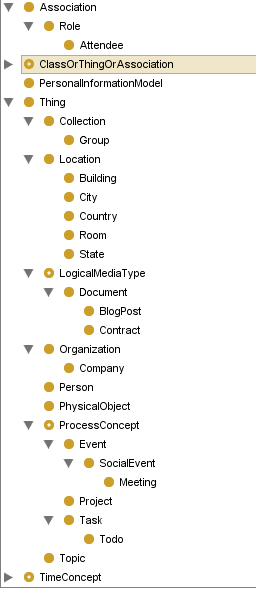
\includegraphics{images/upperclasses.png}
		\caption{Classes in PIMO-Upper}
	\label{fig:upperclasses}
\end{figure}

\begin{description}
%
%    NOTE !!!!!!!!!!!!!!!!!!!!!!!!!!!!!!!
%    These are copied from the ontology, and if not, the
%    descriptions have to be the same in the ontology and here.
%
	\item[Thing] The root class of the upper ontology. Every entity that can be in the direct attention of the user is a Thing.
	\item[Collection] A collection of Things, independent of their class. The items in the collection share a common property. Several usability studies showed that collections are important for PIM. It is recommended to either use the \texttt{pimo:hasPart} or the \texttt{pimo:isTagFor} relation to connect a collection with the Thing it contains\footnote{A Risk Of Change: A clear recommendation to either property may follow in future versions}.
	\item[Group] A group of Persons. They are connected to each other by sharing a common attribute, for example they all belong to the same organization or have a common interest.
	\item [Location] A physical location. Sub-classes are modeled for the most common locations humans work in: Building, City, Country, Room, State. This selection is intended to be applicable cross-cultural and cross-domain. City is a prototype that can be further refined for villages, etc.
	\item [LogicalMediaType] MediaConcepts are logical media types (e.g., a book, a contract, a promotional video, a todo list).  The user can create new logical media types dependent on their domain: a salesman will need MarketingFlyer, Offer, Invoice while a student might create Report, Thesis and Homework.
	\item [Organization] An administrative and functional structure (such as a business or a political party).
	\item [Person] Represents a person. Either living, dead, real or imaginary. In this regards, similar to \texttt{foaf:Person}.
	%\item [PhysicalObject] An object of interest in the physical world. \note{\emph{Knud}: if there is a physical object, how about an abstract object? Love? Language?
%\emph{Leo}: correct. I see a problem with Organozations and Topics, they have
%an overlap with AbstractObject. This can lead to a longer discussion...
%	we should consult sumo. I added this as an open issue at the end.\ref{issue:abstractobject}}	
%	It can be touched, it is concrete and it is of interest to the user. Examples are cars, tables, products and goods of business interest.
	\item[ProcessConcept] Concepts that relate to a series of actions or operations conducing to an end. Sub-classes are defined for Event, SocialEvent, Meeting, Project, and Task.
	\item[Topic] A topic is the subject of a discussion or document. Topics are distinguished from Things in their taxonomic nature, examples are scientific areas.
	\item[Tag] Tag is an abstract marker class to specify which Things in the user's PIMO should be considered useful tags in a tagging system. All Topics are Tags (Topic is a subclass of Tag). Implementations should support the user by using a useful set of Things as Tags, see Section~\ref{sec:tagginginpimo}.
\end{description}

These classes are intentionally kept generic. More specialized ontologies should be used for certain domains of application, see Section~\ref{sec:integratingontologies}. The classes of these ontologies are then  sub-classes of upper ontology classes. 

\subsection{Describing Things with Attributes and Relations}
\label{sec:describingthings}
Conventional RDF statements are used to describe Things. Predicates have to be defined as \texttt{rdfs:Properties} according to the NRL standard. Alternatively, it is also possible to use properties from other modeling languages like OWL or RDFS although we do not encourage this without a proper mapping of existing ontologies to PIMO (see~\ref{sec:integratingontologies}).

Properties that are intended to be editable and visible to end users \textbf{must} be sub-properties of either \texttt{pimo:datatypeProperty} or \texttt{pimo:objectProperty}.

Many NIE and NAO properties can be used from PIMO Things, see Section~\ref{sec:usingnieinpimo}. 

\subsection{Generic Properties in PIMO-Upper}
\label{sec:genericproperties}
The PIMO-upper ontology contains basic relations between Things and a few core attributes for identifying them (described above in Sect.~\ref{sec:identification}). 
These sub-properties of \texttt{pimo:objectProperty} are:
\begin{description}
  \item [\texttt{pimo:related}] is the most generic relation, giving no further indication how Things may be related. Related is defined to have itself as inverse property, 
  it is indirectly a \texttt{nrl:SymmetricProperty}, but does not inherit this attribute to sub-properties. Sub-properties can be asymmetric, depending on the inverse-of relation they define.
	\item [\texttt{pimo:hasPart}] and \texttt{pimo:partOf} model partitive relations. They are inverse. Neither is transitive, because part-of relations used for modelling in the domain of Personal Information Management are vague due to the many contexts of interpretation (a hotel may be part of a trip plan, a trip plan part of a project, but this does not indicate the hotel to be part of the project).
	\item [\texttt{pimo:hasTag}] and \texttt{pimo:isTagFor} connect a Thing of interest with a Tag characterizing it. For example, a meeting can have a project as a tag, or a document has a meeting as a tag, when the goal of the meeting is to discuss the document. After the meeting, the meeting minutes are a new Thing having the meeting as a tag. This is not restricted to meetings but also an organization or a person can have a certain technology as a tag to express that they are working on the topic described by the tag. The relation is not transitive, not symmetric. It is not asymmetric because a thing A may have thing B as tag, and B also A, if both are tags. The range of the \texttt{pimo:hasTag} relation is restricted to the class \texttt{pimo:Tag}. Topic is a subclass of tag. See Section~\ref{sec:tagginginpimo}.
\end{description}

Implementers may use these generic properties directly, or create sub-properties of them
or sub-properties of the more generic \texttt{pimo:objectProperty}.
The main reason to have the generic properties is the semantic meaning of the relations,
which can help to create user interfaces or model domains. 
Ontology authors can ask themselves ``does a new property model a part-of relation or not, does it assign a thing with a topic, or is it a generic relation?'' and then extend one of the generic properties.

For these generic relations, specialized sub-properties are defined when used on specific  classes in the PIMO upper ontology.

\subsection{Refined properties in PIMO-Upper}
\label{sec:pimoupperrelations}
Additional to the above relations, semantically interesting relations between PIMO upper classes are modeled. Especially those which can be used as symmetric or transitive relations for inference.

\begin{description}
	\item[\texttt{pimo:subTopic}] and \texttt{pimo:superTopic} relate Topics to each other. As Topics are an important mean to organize document collections based on a taxonomy, these two predicates are defined. They are inverse of each other and transitive.
	\item[\texttt{pimo:hasOrganizationMember}] and \texttt{pimo:isOrganizationMemberOf} are relations connecting a Person to an Organization.
	\item[\texttt{pimo:hasLocation}] and \texttt{pimo:isLocationOf} relate a locatable Thing with its Location. Locatable is an abstract sub-class of Thing.
	\item[\texttt{pimo:containsLocation}] and \texttt{pimo:locatedWithin} relate two locations within each other. Note that for geographic locations representing a physical space, inclusion is transitive.
\end{description}

\subsection{Tagging Things with Tags}
\label{sec:tagginginpimo}
% Say that PIMO is intended to work as an ontology, but also as a tagging system. When tagging e-mails or other elements, the name of the used tag must be unique. This is to be compatible with existing tagging systems, and to simplify the model. Intended use of TAG is to build a tag-cloud and organization system for the user's documents. Say that all topics are tags and are also arranged in a hierarchy (see next section). Recommend which classes make good tags: classes that exist for a longer time and can be used to classify many documents: topic, collection, group, city, person, organization, project. Say why it won't work without pimo:Tag. The classification system must be smaller than the document collection, to optimize retrieval.
The generic properties described in the last Sections show how Things can be related to each other.
An important aspect of PIMO is to classify Things using ``Tags''. 
Compared to normal PIMO Things, \emph{Tags} have one important additional restriction to make them compatible with Tags from other tagging system (folksonomies and Topic Maps):
\begin{itemize}
	\item The label of a Tag is unique, within the scope of one Personal Information Model.
\end{itemize}
Using Tags, PIMO can be used similar to an existing tagging system.

To extend a Thing to become a Tag, add the type \texttt{pimo:Tag}:
\begin{verbatim}
# The Person Dirk
claudia:DirkHagemann
  a pimo:Person;
# also a Tag
  a pimo:Tag;
# Must define the required pimo:tagLabel
  pimo:tagLabel "Dirk Hagemann".
\end{verbatim}
The \texttt{pimo:tagLabel} is required for all instances of \texttt{pimo:Tag}, and as it is a subproperty of \texttt{nao:prefLabel}, it can replace an existing prefLabel.
The \emph{intended use of Tags} is to build a clear category system for the user's documents. 
Once a Thing is \emph{tagged}, it can be retrieved by finding first the Tag, and then Things associated with the Tag.
A user's Tags are good candidates as first entry points to explore a data space, they can be visualized in a tag cloud or an alphabetical list. Tags can be clustered by type (each has an additional PIMO type), and by hierarchy (Tags can be organized in a part-of hierarchy, Topics are organized in a subTopic hierarchy).

To be useful as classification system, there should be a limited number of Tags to classify the potentially larger amount of documents. 
Examples are Things which exist for a longer period of time and Things that are of much importance to the user. 
Implementations \textbf{should} provide means to use the following as Tags.
\begin{itemize}
	\item All \textbf{Topics} can be considered Tags. This is expressed by the fact that Topic is a subclass of Tag.
	\item \textbf{Collections} work well as Tags, the act of putting something into a collection can be considered an act of tagging.
	\item A \textbf{person}.
	\item A \textbf{group of persons}. 
	\item A \textbf{city}, as there is a limited number of cities a person interacts with. 
	\item \textbf{Projects} are defined as an ``enterprise carefully planned'', the planning and execution of a project may involve tagging many Things as belonging to the project.
	\item A \textbf{task}, as documents may be needed to fulfill the task.
	\item An \textbf{organization} to classify to which organization a person belongs or by which organization a document was published.
\end{itemize}
The process of using an existing Thing as Tag \textbf{may} be automated. For example, a user searching for a possible Tag for a document should be able to pick from a list of existing Tags, and additionally search for Things of the above type to convert them to a Tag (such as a ``more Tags'' button). 
The conversion from Thing to Tag \textbf{may} then be automated and not visible to the user.

Tagging a document is illustrated in the following example, for more details refer to Section~\ref{sec:taggingfiles}.
\begin{verbatim}
claudia:BelfastMeetingPackage a claudia:MeetingPackage, pimo:Tag;
  pimo:tagLabel "Belfast Meeting Package".

claudia:BelfastBusTimetable a pimo:Document;
  pimo:groundingOccurrence <file://home/claudia/doc/tripplan.pdf>;
  pimo:hasTag claudia:BelfastMeetingPackage.
\end{verbatim}

In general, it should be avoided to use \texttt{pimo:Document} instances as Tags.
Typically the amount of documents is high, making them less useful as categorization scheme compared to the above mentioned Thing classes. 
The reason to introduce Tags in PIMO is to allow implementers to separate between categorization scheme and annotated instance base (which is usually a document corpus).
Without a class to mark Tags, it would not be possible to restrict the \texttt{pimo:tagLabel} predicate to a minimum cardinality of one, and also Topics could not automatically be defined as Tags.

\subsection{Topic Hierarchies}
\label{sec:topichierarchies}
% say that PIMO is a taxonomy system comparable to SKOS. The hierarchical ordering of Topics is important to organize the system. Hierarchies are also used to allow semantic search on subtopic structures. add rules.
The methodologies so far allow the description of individual Things with labels, properties, classes, and Tags. 
Besides the view on individuals, their place inside an overall organization scheme of the user can be important --- where is a Thing located in a hierarchy? 
Things can be placed in a hierarchy using the \texttt{pimo:hasPart} relation. 
In an overall hierarchy, the part relation can be confusing, as Things both have a class and can be part of something. For example, \emph{workpackage 2} is \emph{part of } the \emph{CID project}. In a combined hierarchy including class and part-of relations, it would appear at two positions: as instance of workpackage and as part of CID. 

To simplify the system for novice users, it is \textbf{recommended} for implementers to support a \emph{Topic Hierarchy}, where hierarchical part-of structures are shown to end-users. The semantic ``is-a'' relations \textbf{should} be hidden in the Topic hierarchy.
This allows users to model parts of their PIMO as taxonomy.
\begin{itemize}
	\item Each instance of \texttt{pimo:Topic} \textbf{must} either have a \texttt{pimo:hasSuperTopic} relation to another Topic or be defined as root Topic using \texttt{pimo:hasRootTopic}.
	\item All Topics \textbf{must} be connected (indirectly or directly) to a root Topic, or be a root Topic themselves.
	\item User interfaces \textbf{should} render Topics using the hierarchical structure.
	\item Cycles in the super-topic structure are allowed but \textbf{should} be avoided.
	\item A Topic can have multiple super Topics, PIMO allows poly-hierarchical structures.
	\item The \texttt{pimo:subTopic} and \texttt{pimo:superTopic} relations are defined \emph{transitive}. 
	\item When displaying Topics in hierarchical user interfaces, the transitivity of \texttt{pimo:subTopic} \textbf{should} not be inferred. The user experience should be the same when modelling and when browsing the hierarchy.
	\item When searching for Things using the \texttt{pimo:hasTag} relation, the transitivity of \texttt{pimo:subTopic} \textbf{should} be inferred, see below.
\end{itemize}

To support \emph{semantic search} in Topic hierarchies, the following rule for tagging does apply when searching for Things using the hasTag relation (for a detailled description, see Section~\ref{sec:pimorules}):
\begin{verbatim}
CONSTRUCT 
{?x pimo:hasTag ?B.} 
WHERE 
{?x pimo:hasTag ?A. 
?A pimo:superTopic ?B.}
\end{verbatim}

The hierarchical structure of Topics in PIMO is comparable to the modeling in SKOS\cite{SkosStandard}. The \texttt{pimo:subTopic} relation is equivalent to \texttt{skos:narrowerTransitive}.
PIMO requires all Topics to be connected to root Topics, SKOS does not require this in the semantics of \texttt{skos:hasTopConcept}.

\subsection{Creating Personalized Classes and Properties}
\label{sec:customontology}
The predefined classes and properties are intended as a generic basis to be extended.
The user can always create new classes and property types, or existing ontologies can be imported (see Section~\ref{sec:pimomid}).
A number of requirements apply:
\begin{itemize}
	\item The superclass has to be \texttt{pimo:Thing} or a sub-class.
%	\item The property pimo:isDefinedBy has to be set to express that the user created the % class.
	\item The class has to be labelled with \texttt{nao:prefLabel}.
	\item The class has to be related to the user's PIMO with \texttt{pimo:isDefinedBy}.
\end{itemize}

Similarly for custom properties:
\begin{itemize}
	\item The property has to be labelled with \texttt{nao:prefLabel}.
	\item The property has to be related to the user's PIMO with \texttt{pimo:isDefinedBy}.
\end{itemize}
For properties that relate two things, the following applies:
\begin{itemize}
  \item The property \textbf{must} be a sub-property of \texttt{pimo:objectProperty} (either directly or indirectly via inference).
	\item The super-property \textbf{should} be one of \texttt{pimo:related}, \texttt{pimo:hasTag}, \texttt{pimo:isTagFor}, \texttt{pimo:hasPart}, or \texttt{pimo:partOf}.
	\item An inverse property \textbf{must} be defined. Inverse properties define the semantic meaning in both ways, which is required for 
user interfaces showing relations.
\end{itemize}
For custom properties that have \emph{a literal or datatype as range} the following applies:
\begin{itemize}
  \item They must be a sub-property of \texttt{pimo:datatypeProperty}.
  \item Inverse properties should not be defined (as Literals cannot be subject of statements, inverse does not apply anyway).
\end{itemize}

For all custom-created properties and classes, 
modification dates \textbf{must} be set.

\subsection{Collections of Things}
\label{sec:collections}
In Personal Information Management, grouping multiple Things into one collection is a crucial feature. Today's hierarchical file systems are a good example: a folder can be created to contain multiple elements. Later, actions on this folder, such as compressing it, or deleting it are supported.
The generic \emph{has Part} relation provides the semantics of putting a Thing into another Thing. For usability reasons, we also provide a class \texttt{pimo:Collection} to be used for generic collections of multiple items.

Applications that want to present the complex possibilities of PIMO in a simpler way can offer collections. 
First, an instance of the class \texttt{pimo:Collection} is created. Then, elements are added to the collection using the \texttt{pimo:hasPart} relation. 
A typical application of collections is the list of ``Favourites'' containing recently used and important resources.

Collections are unordered, the ordering of items inside the collection can be done using alphabetical order, time, geographic location (if they are locatable), or type.

Tags are another simplification, described below in Section~\ref{sec:taggingfiles}.

%\begin{itemize}
%	\item collections are unordered
%	\item temporal order is expressed using implizit modeling (the time difference is implicit and has to be calculated for explizit knowing it for sorting)
%	\item in science, different sorting systems are described: geographical, alphabetically,  by Time, by Categories, by Hierarchy.  (Location, Alphabet, Time, Category, and Hierarchy, known as LATCH  cite R. Wurman, D. Sume, and L. Leifer, Information Anxiety 2, Que, 2000.)
%	\item Latif and Tjoa, 2006 \cite{Latif+2006} have existing systems are build on LATCH, and additionally refine it saying that hierarchy is often taxonomic and that people are an important ordering factor, as also does Dengel2006.
%	\item That said, we see that ordering is dependent on the view in the application and on the attributes of the elements, there is a reason WHY the elements are ordered in a way based on their attributes. For PIMO, we do not provide an explicit sort order (before/after) relations, this can be added by implementers as extensions. The NEPOMUK Conceptual Elements model, developed by Max V�lkel and Heiko Haller defines the standards for ordering. On the level of PIMO, ordering of items in a collection is implizit by the attributes of the items in the collection and handled by the user interface, by showing the elements in whatever order is appropriate.
%	\item The Collection class can be used to model collections of items that share a common attribute. 
%	\item Members of collection are modeled using hasPart.
%\end{itemize}

\subsection{Modeling Associations and Roles in PIMO}
\label{sec:roleBasedModeling}
Often there is a need to add meta-data about a relation, for example the date of creation of a relation. 
In RDF, this is typically done using reification, and then adding meta-data about the 
reified Statement using an instance of the class \texttt{rdf:Statement}. 
A problem with reification is that when using the generic class \texttt{rdf:Statement}
to represent it, there are no guidelines which properties are now suitable to annotate the statement.
More precise sub-classes of Statement would solve this.
Another problem is that \emph{n-ary} relations cannot be expressed with triple statements.

In PIMO, \textbf{Associations} are used to add metadata about relations and to create
n-ary relations. They are entities representing the relation of multiple Things with each other.
Each Thing part of an Association is related to the association using the \texttt{pimo:associationMember} property or more precise sub-properties of it.

As an example, the fact that Claudia attended a meeting can be expressed using the \texttt{pimo:Attendee} role.

\begin{verbatim}
claudia:AttendsInitialMeetinginBelfast a pimo:Attendee;
  pimo:attendingMeeting claudia:InitialMeetinginBelfast;
  pimo:roleHolder claudia:Claudia.
\end{verbatim}

Here, the class \texttt{pimo:Attendee} is a sub-class of \texttt{pimo:Association}
and represents the association as such (``this is an association between a person and a meeting''). The two relations used are sub-properties of \texttt{pimo:associationMember} and identify the two Things to relate, the specific relations determine the role taken by each Thing. 
New sub-classes of association can be created when needed, also new sub-properties
of \texttt{pimo:associationMember} for more specific roles. 

Associations are elements of a user's PIMO and \textbf{must} be connected to the user's PIMO with a \texttt{pimo:isDefinedBy} relation.
Modification dates are to be handled the same way as with Things (see Section \ref{sec:changedates}).

\section{Connecting PIMO to Information Elements}
\label{sec:pimoVSnie}
In the last section, the Things created within a user-PIMO were described.
They are to be unique, described with defined ontologies,
and ought to be identified well.
The next step is to connect these to the files, e-mails, and other Information Elements
which exist in the user's PSI.
These are ambiguous, described in various ontologies, and in general more chaotic when compared to the user-PIMO.
The crucial point is to use Things as organization scheme to classify and integrate
existing data found in a PSI.

The first step is to \textbf{connect Things to Information Elements} that represent them.
As described above (Section \ref{sec:identification}), the \texttt{pimo:groundingOccurrence}
and \texttt{pimo:occurrence} relations are to be used to connect them.
This connection has the semantics of a unification --- both the Thing and the Information Element represent the same real-world entity. 
But the Thing is the unique, static representation that should be used to annotate the entity.
Implementations \textbf{should not} allow the users to annotate Information Elements directly, instead it is \textbf{recommended} to connect the Information Element to a Thing using \texttt{pimo:groundingOccurrence} and then annotate the Thing.
The rationale is that Information Elements can change their URI, be deleted or moved, and then the annotations may be disconnected from the described resource. 

Creating a Thing for each annotated document will result in vast amounts of instances in the sub-classes of \texttt{pimo:Document}, as users can likely have access to thousands (sometimes millions) of documents. To navigate effectively through such large structures, PIMO Topics can be used to annotate documents using the \texttt{pimo:hasTag} relation.

How to annotate documents using PIMO is described in Section \ref{sec:taggingfiles}.

\subsection{Connecting Things and Classes to Folders}
\label{sec:containers}
Things can also be connected to folders in the file-system to express that
these folders contain information related to the thing. 
Use the \texttt{pimo:hasFolder} relation to connect a Thing or a Class with a folder.
The semantic meaning of this relation is not formally restricted but open to be used in various ways.
For folders connected to Things, it is \textbf{recommended} 
to interpret the content of the folder as ``having the Thing as topic''.
Implementers \textbf{may} add a \texttt{pimo:hasTag} relation between the Things inside the folder and the Thing. 

For folders connected to Classes, it is \textbf{recommended}
to interpret the content of the folder as ``being an instance of the Class''.
Implementers \textbf{may} add a \texttt{rdf:type} relation between the Things inside the folder and the Class.

In all cases, files or other information elements in folders have to 
be represented as Things first, before further annotation (see Section \ref{sec:creatingthingalgorithm}).

The property \texttt{pimo:hasFolder} \emph{can} be used by implementers
to suggest folders for information elements --- if an information element
is annotated with a \texttt{pimo:hasTag} relation to a topic that is connected
to a folder, this is an indication to move the element to the folder, if needed.

\subsection{Integrating Facts about Things}
\label{sec:integratingfacts}
The unification of multiple Information Elements into one Thing is also 
on the level of facts, RDF statements.
To answer the question ``when did I last communicate with people shown on this
picture'' can only be answered when facts from multiple sources (e-mails, photos, photo annotations and the user-PIMO) can be queried as one model.
The statements about the Information Elements connected to a Thing via \texttt{pimo:groundingOccurrence} and \texttt{pimo:occurrence} can be \textbf{superimposed} to the Thing.
The exact rules are given in Section \ref{sec:creationrules} and directions
how to use them are in Section \ref{sec:unification}.

Through this process, a view on the data is generated.
The user can get an overview of all existing data --- in an integrated way --- and then
drill down into specific occurrences.
In this view, it is possible that a Thing has multiple classes (as \texttt{rdf:type}),
one from the level of PIMO ontologies and others from the integrated Information Elements.
In the example given in Section \ref{sec:unification}, 
Dirk Hagemann is inferred to be both a \texttt{pimo:Person}
and a \texttt{pimo:PersonContact}. 
The two classes are not required to be sub-classes of each other.
To get a coherent and meaningful view, the class of the InformationElement (or related resource) \textbf{may} be related to a PIMO class using the \emph{pimo:hasOtherConceptualization} relation, as described later in Section~\ref{sec:integratingontologies}.

It is not required that the used ontologies are formally aligned and mapped.
Rather, it is assumed that the user will be able to interpret the statements based on his knowledge about the data in his PSI.

The details about the integration of facts are given in Section \ref{sec:unification} on \emph{unification}.
 
\section{PIMO-group level: Group and Domain ontologies}
\label{sec:pimomid}
% In this section we introduce the idea of specializations of 
% PIMO upper that are shared amongst companies and groups.
% COPIED FROM SauermannElstDengel2007
The upper (foundational) level of \pimo just makes a few, basic
ontological statements about Things which exist on a Semantic Desktop, \ie Things which
are essential in a knowledge worker's mental model.
In order to avoid a \emph{cold start problem}
\footnote{The problem of cold starts is well known in knowledge-based systems: In the beginning a system, such as a shell, has little or no information and therefore doesn't seem to be useful to a new user. 
Consequently, they are not motivated to invest in using and feeding the system with new
information, which again would be a prerequisite for it to be \emph{more} useful. Enter vicious cycle...} 
with PIMO-based
applications, more ontologies defining concepts shared within groups 
or modeling domains are needed.
The user's company and its organizational structure may be such a domain, or a shared public ontology.
Classes are refinements of PIMO-Upper, allowing an integration
of various domain ontologies via the upper layer.

In the following section, recommendations are given how to model group and
domain level ontologies.

%\section{Mapping ontologies to PIMO-upper}
\section{Extending PIMO}
\label{sec:integratingontologies}
%\note{Knud: I changed the title, because I think this chapter is not only about mapping ontologies, but more generally speaking about how to extend PIMO for one's needs. Leo: perfect.}
%\note{Leo: this section should be either merged with the previous one, or the previous one removed. Both is fine, removing above is probably nicer.}
Out of the box, PIMO is kept sufficiently simple and only contains relatively few classes and properties. This was done in order to ensure that the ontology is general enough to apply to almost any relevant domain. 
% removed. see https://dev.nepomuk.semanticdesktop.org/ticket/534
%At the same time, PIMO contains enough basic elements to allow the user to start working straight away and prevent the cold start phenomenon. 
However, as soon as the set of pre-existing classes and properties becomes too narrow and confining, it is a very simple matter to extend PIMO and add domain-specific extensions, or map external ontologies onto PIMO. E.g., PIMO can easily be extended to express the organizational structure of the user's workplace, a biological classification system, or to include a PIMO-version of the BibTeX vocabulary.
These \emph{domain ontologies} differ from \emph{personalized classes and properties} (see Section \ref{sec:customontology}) by the fact that they are not created by the user,
but created by a third party for multiple users.
\subsection{Refining Elements of PIMO-upper} % (fold)
\label{sub:subclassing_pimo_upper}
Creating group--level ontologies is a simple matter of \textbf{defining new sub-classes of PIMO-upper classes (see Sect.~\ref{sec:pimoUpperClasses}) or sub-classing \texttt{InformationElement} classes}. 
If needed, new properties can also be added, which apply to the new classes via domain or range.
Importing created \emph{group--level ontologies} into a user's PIMO is described in the next Section (\ref{sec:importingontologies}).

\paragraph{Classes} % (fold)
\label{par:classes}
 
%\note{Leo 13.12.: The individual values for Grades are a good example where instances must be added to domain ontologies. Could you add the grades such as teaching:GradeA, teaching:GradeB, teaching:GradeC, ... teaching: GradeF and give them preflables ``A''..''F'' ? This also looks good in N3. The argumentation is that teachers can then search for Students having grade ``A''.. etc ... and these are shared amongst teachers.}
%\note{Knud, 05.01: Done! :)}
%\note{Leo 13.12: in general, instances can be added to domain ontologies when they are shared amongst all users, for example a school may publish a domain ontology with instances for all teachers and personnel, and typical courses for each year to take the burden of modeling away from the teachers}
% Leo: commented out above notes, they are DONE!
As an example, you may work in the domain of teaching and training, and therefore want to extend PIMO with elements specific for this domain, such as \emph{courses}, \emph{lessons}, \emph{teachers} or \emph{students}. In this case, you would look for existing PIMO-upper classes which could be considered generalizations of your new classes. E.g., a course would be a sub-class of \texttt{pimo:ProcessConcept}, training lessons could be a sub-class of \texttt{pimo:Meeting}, teachers and students could be sub-classes of \texttt{pimo:Person} (or \texttt{pimo:Role} --- role-based modeling is discussed in Sect.~\ref{sec:roleBasedModeling}) and training material a sub-class of \texttt{pimo:Document}. Since all pre-existing PIMO-upper classes derive from \texttt{pimo:Thing}, all your new classes automatically do as well (except for roles: \texttt{pimo:Role} is not a sub-class of \texttt{pimo:Thing}). 

There could also be cases where no existing PIMO-upper class seems to apply to your new class --- in this case, the new class would directly derive from \texttt{pimo:Thing}. Consider, e.g., that you want to include the concept of \emph{grades} in your PIMO. There isn't really a good pre-existing superclass for grades in PIMO-upper, so your new \texttt{Grade} class would be a direct sub-class of \texttt{pimo:Thing}.

Even if there might be a potential superclass, it may be wise to postpone this decision if one isn't completely sure, and instead just sub-class \texttt{pimo:Thing}. It is always easier to add a superclass relationship later, rather than make a bad decision now and then have to deal with incorrect data at a later stage.

If needed, the new classes can also have sub-class relationships into other ontologies, such as other NIE-based ontologies or completely different ontologies such as WordNet\footnote{\url{http://wordnet.princeton.edu/}}, SUMO\footnote{\url{http://www.ontologyportal.org/}}, or Dolce\footnote{\url{http://www.loa-cnr.it/DOLCE.html}}.

% paragraph classes (end)

\paragraph{Instances} % (fold)
\label{par:instances}

In some cases, you will also want to add instances of classes to the ontology you are integrating with PIMO. This makes sense if those instances are shared and used among a many users. An example are actual grades that a teacher might gives their students, such as grades from A--F. Each such grade (\texttt{teaching:GradeA}, \texttt{teaching:GradeB}, etc.) is an instance of the class \texttt{Grade}, but since those instances will be used by all teachers and students, they can become part of the teaching ontology. Similarly, if a school decides to introduce the teaching ontology, they might include instances for all their teachers, students, classes, courses, etc.

% paragraph instances (end)

\paragraph{Properties} % (fold)
\label{par:properties}

New properties can then refer to the new classes via domain or range and thus further specify them. Examples are the relation between courses and teachers/instructors (e.g., \texttt{teachesCourse(Teacher, Course)}) or between course material and a course (e.g. \texttt{courseMaterialFor(CourseMaterial, Course)}). This example is illustrated graphically in Fig.~\ref{fig:extensionExampleTeaching}, as well in N3 source code in Fig.~\ref{fig:extensionExampleTeachingN3}. This approach is a \textbf{typical example of how to integrate domain ontologies for specific application areas into PIMO}.

There are some general guidelines for introducing new properties:
\begin{itemize}
	\item Properties which connect two \texttt{pimo:Thing}s (or sub-classes) should be defined as sub-properties of \texttt{pimo:related}, \texttt{pimo:hasTag}, \texttt{pimo:isTagFor}, \texttt{pimo:hasPart}, or \texttt{pimo:partOf} (see Sect.~\ref{sec:genericproperties}). By relating new, specialized properties to the more generic PIMO properties, the new ontology can integrate better with existing desktop environment. When not extending the generic properties, at least new properties should exted \texttt{pimo:objectProperty}.
	\item All new object-properties \textbf{must} define an inverse property, as required
	in Section~\ref{sec:customontology}.
	\item Identifying properties (such as a name) that have domain \texttt{pimo:Thing} and a literal range should be mapped as sub-properties of \texttt{nao:identifier}. An example is give in Fig.~\ref{fig:bibtexExample}.
	\item 
% Leo 8/1: removed the note, the fix seems to be accepted by Knud.
%\note{\emph{Knud}: I don't understand this at all. Leo: I splitted it up to two items and explained the concept of referencing occurrences a little.}
	Some new properties may be defined as sub-properties of \texttt{pimo:referencingOccurrence} (see Sect.~\ref{par:referencingOccurrence}). This is true for all object properties (i.e., properties which have a resource range and not a literal range) which describe or identify the subject in an unambiguous way. In other words, the object resource   exclusively describes the subject. A typical example is \texttt{foaf:homepage}: two different people would most likely not have the same homepage (ignoring exceptions such as family homepages). If, however, we come across two different RDF resources which have the same \texttt{foaf:homepage}, we can assume that they describe the same real-life person.
	  \item A frequent situation in Semantic Web and Semantic Desktop scenarios is that the same real-life object (i.e., a person, country, project, etc.) is defined as a resource in many different ontologies. The PIMO property \texttt{pimo:hasOtherRepresentation} is used in such cases. If your new ontology contains a property which expresses a similar (more specific) relation between resources, then it should be a sub-property of \texttt{pimo:hasOtherRepresentation} (see Sect.~\ref{par:otherRepresentation}). In the vanilla SW world, a similar property is \texttt{rdfs:seeAlso}.
\end{itemize}

% paragraph properties (end)

\begin{figure}
  \begin{center}
    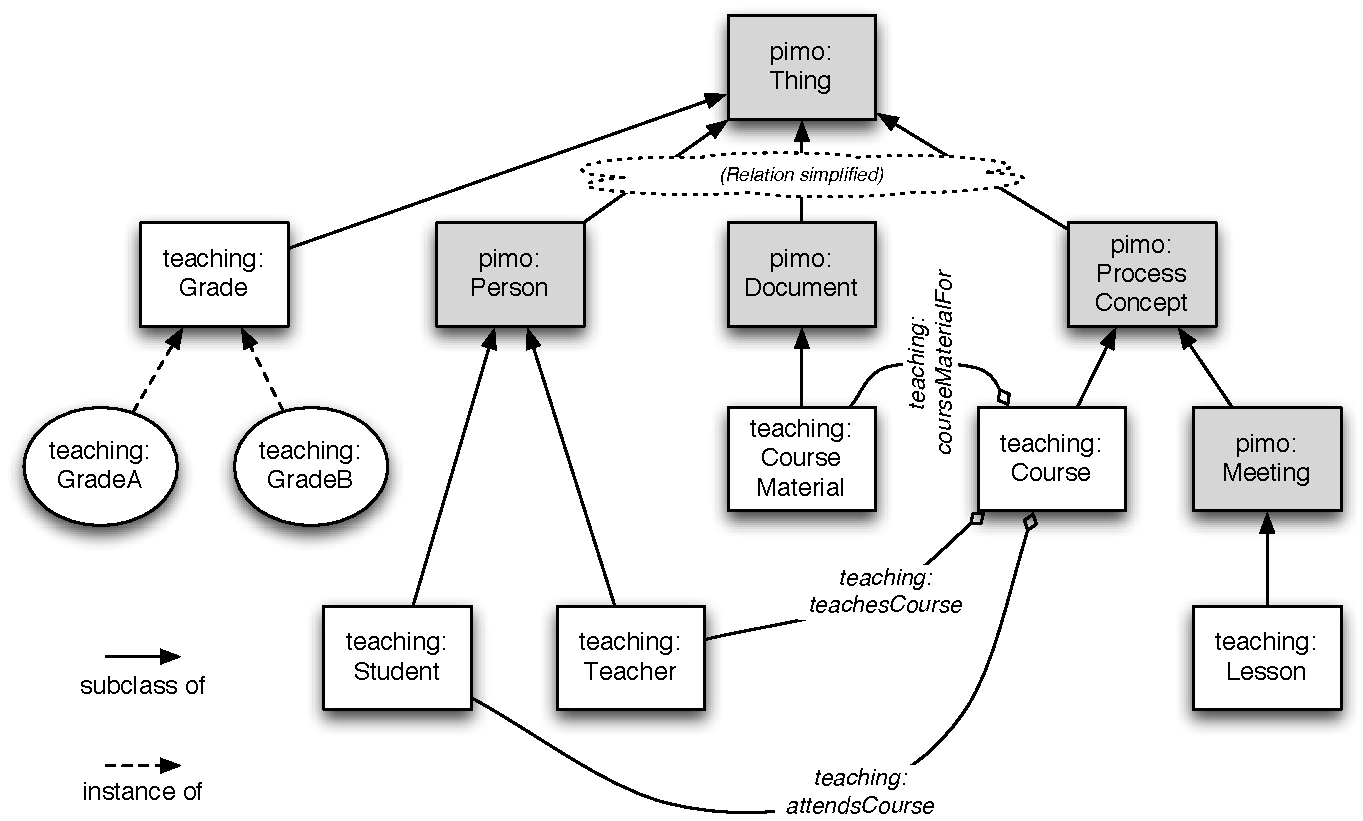
\includegraphics[width=\linewidth]{images/PIMOextensionExample-Teaching}
    \caption{Extending PIMO with new classes, properties and instances for the domain of teaching}
    \label{fig:extensionExampleTeaching}
  \end{center}
\end{figure}

\begin{figure}
  \begin{center}
	\begin{verbatim}
# new classes:
   teaching:Grade a rdfs:Class;
      rdfs:subClassOf pimo:Thing.

   teaching:Student a rdfs:Class;
      rdfs:subClassOf pimo:Person.

   teaching:Teacher a rdfs:Class;
      rdfs:subClassOf pimo:Person.

   teaching:CourseMaterial a rdfs:Class;
      rdfs:subClassOf pimo:Document.

   teaching:Course a rdfs:Class;
      rdfs:subClassOf pimo:ProcessConcept.

   teaching:Lesson a rdfs:Class;
      rdfs:subClassOf pimo:Meeting.

# new properties and their inverse:
   teaching:courseMaterialFor a rdf:Property;
      rdfs:subPropertyOf pimo:partOf;
      rdfs:domain teaching:CourseMaterial;
      rdfs:range teaching:Course;
      nrl:inverseProperty teaching:hasCourseMaterial.
   teaching:hasCourseMaterial;
      rdfs:subPropertyOf pimo:hasPart;
      rdfs:domain teaching:Course;
      rdfs:range teaching:CourseMaterial;
      nrl:inverseProperty teaching:courseMaterialFor.

   teaching:teachesCourse a rdf:Property;
      rdfs:subPropertyOf pimo:related;
      rdfs:domain teaching:Teacher;
      rdfs:range teaching:Course;
      nrl:inverseProperty teaching:taughtBy.
   teaching:taughtBy a rdf:Property;
      rdfs:subPropertyOf pimo:related;
      rdfs:domain teaching:Course;
      rdfs:range teaching:Teacher;
      nrl:inverseProperty teaching:teachesCourse.
      
   teaching:attendsCourse a rdf:Property;
      rdfs:subPropertyOf pimo:related;
      rdfs:domain teaching:Student;
      rdfs:range teaching:Course;
      nrl:inverseProperty teaching:attendeeStudent.
   teaching:attendeeStudent a rdf:Property;
      rdfs:subPropertyOf pimo:related;
      rdfs:domain teaching:Course;
      rdfs:range teaching:Student;
      nrl:inverseProperty teaching:attendsCourse.

# new instances:
    teaching:GradeA a teaching:Grade;
      nao:prefLabel "A".

    teaching:GradeB a teaching:Grade;
      nao:prefLabel "B".

    ...
	\end{verbatim}
    \caption{Extending PIMO with new classes, properties and instances for the domain of teaching --- N3 code}
	\label{fig:extensionExampleTeachingN3}
\end{center}
\end{figure}

\paragraph{Inheritance} % (fold)
\label{par:inheritance}

Sub-classing any class from PIMO (whether it be existing classes from PIMO-upper or classes that have been added later) also means that the new sub-class can be used with the same properties that have been defined with its superclass. Remember that NRL has a closed world assumption, and not an open world assumption, as RDFS traditionally has. In NRL\footnote{\url{http://www.semanticdesktop.org/ontologies/nrl/}}, ontologies can be used to validate statements.
%\note{reference to NRL spec --- 05.01.08, done}
E.g., if the property \texttt{name(pimo:Person, String)} has been defined, and if we define our new class \texttt{teaching:Student} to be a sub-class of \texttt{pimo:Person}, then this will allow us to use \texttt{name} with instances of \texttt{Student} as well - an NRL validator will permit this, because all instances of \texttt{Student} are also instances of \texttt{Person}. An example of this is shown in Fig.~\ref{fig:propertyInheritance}: this concept is very similar to the idea of inheritance in object-orientation, even though strictly speaking it is not the same.

% paragraph inheritance (end)

\begin{figure}
  \begin{center}
	\begin{verbatim}
		
   pimo:name a rdf:Property;
      rdfs:Domain pimo:Person;
      rdfs:Domain rdfs:Literal.
		
   teaching:Student a rdfs:Class;
      rdfs:subClassOf pimo:Person.

   knud a teaching:Student;
      pimo:name "Knud M�ller".

	\end{verbatim}
    \caption{``Inheritance'' of properties}
	\label{fig:propertyInheritance}
\end{center}
\end{figure}

% subsection subclassing_pimo_upper (end)

\subsection{Markup for the new ontology}
\label{sec:extendingontologymarkup}
The teaching ontology still needs to be defined as proper NRL ontology
to be usable with PIMO. The ontology \textbf{must} to be identified via its URI
and the author of the ontology can be added
as \texttt{nao:creator}.

\begin{verbatim}
teaching:TeachingOntology a nrl:Ontology;
 nao:creator teaching:TeachingOntologyCreator.

teaching:TeachingOntologyCreator a nao:Party;
 rdfs:label "Knud M�ller".

\end{verbatim}

\subsection{Information Elements} % (fold)
\label{sub:information_elements}

An important feature of the NEPOMUK ontology architecture is the fact that it is divided into two tiers: the PIMO tier and the Native Structures tier, as defined in the NEPOMUK Information Element Ontology (NIE)\footnote{\url{http://www.semanticdesktop.org/ontologies/nie/}} and its sub-ontologies, such as the NEPOMUK File Ontology (NFO)\footnote{\url{http://www.semanticdesktop.org/ontologies/nfo/}}.
%\note{reference to NIE spec --- 05.01.08, done}
While the former covers the internal mental model of a user or an organization (people, events, projects, etc.), the latter covers the physical representations of data (address book entries, calendar entries, files, etc.). Obviously, there are numerous connections between the tiers: people are represented by address book entries, events appear in the calendar, projects have files associated to them.

Whenever classes that are introduced to PIMO have a physical representation on the user's desktop, a connection to NIE must be modeled as well. Consider the example of the teaching ontology above: Such an ontology will contain classes for Things like exams and essays. Those classes belong to the PIMO tier. Their representation within the computer --- e.g., as text files --- belongs to the native structures tier. Or, in a more complex case, the new ontology could very well come with a specialized application, such as a Training Course Manager, where users can assign attendees to trainings, etc. In this case, people and courses (PIMO tier) would be represented by the application as application-specific data structures or information elements (native structures tier). In both cases a link from the new PIMO classes to the information elements represented with NIE is required to fully exploit the possibilities of the semantic desktop.

% subsection information_elements (end)

%\note{Knud, 05.01.08: I decided to drop the Author class in the BibTeX example. Authors should really just be pimo:Persons, not a subclass thereof.
%Leo, 8/1: OK, DONE}

As a second example, we can consider an ontology for scientific publications. This ontology (which would probably be based on Bib\TeX), would come with classes such as \texttt{Article} or \texttt{Book} and relations between them like \texttt{bookContainsArticle} or \texttt{hasAuthor}. For the integration into PIMO, \texttt{Article} would most likely become a sub-class of \texttt{pimo:Document}. 
Documents have	two types: one which anchors them in the PIMO tier, and one which anchors them in the native structures tier.
The \texttt{pimo:LogicalMediaType} (and its sub-classes, e.g., \texttt{pimo:Document}) captures how a document is interpreted by the user and belongs to the PIMO tier. Logical media types can be contracts, invoices, assignments, invitations, law texts, etc. 
The other type, which is the \texttt{nfo:Document} type, captures how the system interprets the document, and belongs to the native structures tier.
This is the physical document type as modeled by NIE.
Instances of a logical media type can have various representations in the native structures tier: 
for example, a text interpreted as an invoice by the user can either be an \texttt{nfo:PlainTextDocument} or an \texttt{nfo:PaginatedTextDocument}. 
Vice-versa, one physical type can be used to represent both an invitation or an invoice, which are different logical media types.
Keeping this this separation of content and representation in mind, one can model concrete documents having two types, one on each tier.

\begin{figure}
  \begin{center}
\begin{verbatim}
bibtex:Article a rdfs:Class;
 # PIMO tier: interpreted by the user as nie:Document
 rdfs:subClassOf pimo:Document; 
 # native structures tier: interpreted by the system as nfo:TextDocument
 rdfs:subClassOf nfo:TextDocument. 

bibtex:hasAuthor a rdf:Property;
 rdfs:subPropertyOf pimo:related;
 rdfs:subPropertyOf nfo:creator;
 rdfs:domain bibtex:Article;
 rdfs:range pimo:Person.
 
bibtex:hasLCCN a rdf:Property;
 rdfs:subPropertyOf nao:identifier; \# add an identifier
 rdfs:domain bibtex:Article.
\end{verbatim}
    \caption{A Bib\TeX-based PIMO extension for scientific publications}
	\label{fig:bibtexExample}
\end{center}
\end{figure}
%bibtex:Author a rdfs:Class; 
% # this adds properties like Name
% rdfs:subClassOf pimo:Person. 

\subsection{Extension by Sub-classing from External Classes} % (fold)
\label{sub:extension_by_subclassing_from_external_classes}

\textbf{Another possibility is extending existing PIMO-upper classes by sub-classing them from external classes.} \emph{This is discouraged}. For example, if the class \texttt{pimo:Person} was defined a sub-class of \texttt{nco:PersonContact} and \texttt{pimo:Organization} a sub-class of \texttt{nco:OrganizationContact}, all instances of these classes would automatically be inferred to be \texttt{pimo:Thing}s. However, those instances would probably not have some of the properties required by the \texttt{Thing} defined, which would render the imported data invalid. 
Similarly, when a mapped class X has cardinality restrictions on its properties (such as required properties), adding X as new superclass to an existing PIMO class can render the instances of the PIMO class invalid. 

% subsection extension_by_subclassing_from_external_classes (end)

\subsection{Summary} % (fold)
\label{sub:summary}

The very condensed summary to extending PIMO and mapping frome existing ontologies to PIMO is the following:

\begin{itemize}
  \item Make classes sub-classes of PIMO-upper classes.
  \item Make properties sub-properties of PIMO-upper properties.
	\item Relations: Links between Things have to be browseable, properties should have inverse relations defined (see \cite{rohmer2005})
	\item Extensibility: Users are free to add new relation types and new classes (see \cite{rohmer2005})
\end{itemize}

% subsection summary (end)

\section{Importing Domain Ontologies into a User's PIMO}
\label{sec:importingontologies}
%\note{Written by Leo, but Knud: feel free to mash it up}
Once modeled, the new domain ontology such as the teaching ontology in the previous examples can be made available publicly for others, for example by publishing it on the Web. A good reference for doing this is \emph{Best Practice Recipes for Publishing RDF Vocabularies}~\cite{SWBPVocabularyRecipes}.

% adressing
Semantically, an imported ontology is captured using a \texttt{nrl:imports} statement.
When a user imports a domain ontology, this statement \textbf{should} be added.

{\small
\begin{verbatim}
claudia:Pimo nrl:imports teaching:TeachingOntology.
\end{verbatim}
}

%Importing the ontology to a Sematic Desktop or other Personal Information Management system can then be done by downloading the ontology file and storing it into the RDF store where the PIMO of the user is kept.
% Stuff like downloading is outside the scope of PIMO and really has no place in the PIMO specification
Once the user of a Semantic Desktop system imports an external PIMO into their own desktop, all new classes (which are sub-classes of \texttt{pimo:Thing}) \textbf{should} become available to them as if they had created those classes themselves.
Instances, on the other hand, are not automatically available.
As said in the introduction, the scope of a PIMO for an individual user is to model data that is within their own attention and needed for knowledge work or private use.
However, when importing external ontologies or knowledge bases, not all instances may be of interest to the user. As with imported information elements, a separate Thing is created to represent the imported resource within the PIMO of the user and connected to the imported instance using \texttt{pimo:hasOtherRepresentation}\footnote{An alternative would be to treat all Things present in the RDF data available of the user as if they were created by the user, imported or not. This has the drawback that it allows to represent the same real-world entity twice, first in the imported domain ontology and second in the user's own PIMO.}.
Before creating a new Thing for an imported instance, the PIMO of the user has to be checked if the entity is already represented as a Thing, as indicated above in Section~\ref{sec:creatingthingalgorithm}.
Once represented as a Thing in the user's PIMO, it is possible to assign a personal identifier to it, annotate it, and use it. 

Implementations \textbf{must} automate the importing process. The user should be able to interact with imported Things as if they were created by themselves. 

\begin{comment}
LEO: THIS COMMENTED OUT NOW, ITS TOO SCIENTIFIC.
\section{Design Rationale}
\label{sec:designrationale}
In this section the design rationale behind \pimo and the sources which influenced us are described. 
% COPIED FROM SauermannElstDengel2007
%The motivation for creating the PIMO is to find a language to name the terms
%that are relevant to a knowledge worker and to have ways to express facts about
%these terms. Once this language is defined and formalized in the ontological
%description of the PIMO, it can be used to translate existing resources, and to
%express information about them. The PIMO is a user-centric view on existing
%documents, domain ontologies, and web data sources.
%
%While the organization asks for universally applicable and standardized
%persistent structures, processes, and work organizations to achieve and
%maintain universally accessible information archives, the individual knowledge
%worker requests individualized structures and flexibility in processes and work
%organization in order to reach optimal support for the individual activities.
%
The vision behind this work is that a \emph{Personal Information Model} reflects and captures a user's
personal knowledge, \eg about people and their roles, about organizations, processes,
things, and so forth, by \emph{providing the vocabulary} (concepts and their relationships)
required for expressing it as well as concrete instances. In other words, the domain of a
\pimo is meant to be ``all Things and native resources that are in the attention of the
user when doing knowledge work''.
\note{Knud, 07.01.08: Probably quickly explain what native structures are?}
Though ``native'' information models and structures are
widely used, there is still much potential
for a more effective and efficient exploitation of the underlying knowledge. We think that,
compared to the cognitive representations humans build, there are mainly two shortcomings
in native structures:
\begin{itemize}
  \item \emph{Richness of models}: Current state of cognitive psychology
  assumes that humans build very rich models, encoding not
  only detailed factual aspects, but also episodic and situational
  information. Native structures are mostly taxonomy- or
  keyword-oriented.
  \item \emph{Coherence of models}: Though nowadays (business)
  life is very fragmented humans tend to interpret situations as a
  coherent whole and have representations of concepts that are comprehensive
  across contexts. Native structures, on the other hand, often
  reflect the fragmentation of multiple contexts. They tend to be
  redundant (i.e., the same concepts at multiple places in
  multiple native structures). Frequently, inconsistencies are the
  consequence.
\end{itemize}

The \pimo shall mitigate the shortcomings of native structures by providing a
\emph{comprehensive model} on a \emph{sound formal basis}.

% next snip
%When building concrete \pimos, we now have the
%problem of two, potentially conflicting demands: On the one hand, we want to give the user
%the opportunity to span his information space largely in the way \emph{he} wants. The
%\pimo should model \emph{his} mental models. In consequence, we cannot prescribe much of
%this structure. On the other hand, ``empty'' systems often suffer from the cold
%start problem, being not accepted by user when not already equipped with some initial content.
%Using a multi-layer approach (see also \cite{Sauermann+2006d}), we try to find a balance through providing 
%the presentational basis as given, which users \emph{can} incorporate or extend:
%by a layered approach to \pimos : The representational basis
%as well as the basic dimensions of a \pimo are pre-given, but flexible enough for simple as
%well as more advanced modeling. Lower levels are meant as a proposition; when establishing
%an individual \pimo, users \emph{can} incorporate them into their model if they find them
%adequate and useful, but they don't have to. In the following, we briefly sketch the
%proposed \pimo layers:

% NOTE: THIS IS BAD, PIMO-MID IS a FORBIDDEN WORD and therefore replaced with XXXXXXX
%\subsection{PIMO-Basic, PIMO-Upper, PIMO-XXXXXXX and Domain Ontologies}
%Apart from the native structures, the mental models are represented using a multi-layer
%approach. These layers are:
%\begin{itemize}
%  \item PIMO-Basic: defines the basic language constructs. The class
%  pimo-basic:Thing represents a super-class of other classes.
%  \item PIMO-Upper: A domain-independent ontology defining abstract sub-classes of
%  Thing. Such abstract classes are PersonConcept, OrganizationalConcept,
%  LocationConcept, Document, etc.
%  \item PIMO-XXXXXXX: More concrete sub-classes of upper-classes. The
%  mid-level ontology serves to integrate various domain ontologies and provides
%  classes for Person, Project, Company, etc.
%  \item Domain ontologies: A set of domain ontologies where each describes a
%  concrete domain of interest of the user. The user's company and its
%  organizational structure may be such a domain, or a shared public ontology.
%  Classes are refinements of PIMO-XXXXXXX and PIMO-Upper, allowing an integration
%  of various domain ontologies via the upper layers.
%  \item PIMO-User: the extensions of above models created by an individual for
%  personal use. Classes, properties and Things are created by the user.
%\end{itemize}

% END OF SauermannElstDengel2007
\end{comment}


\section{Practical Directions on Using PIMO}
In this section, a few issues that will arise in actual PIMO usage are discussed. For each of these issues, we will suggest a recommended way of handling them. Even though those things are not strictly speaking part of the ontology, they are part of the standard defining how to use the PIMO ontology in applications.
Implementers \textbf{should} conform to these directions.

\subsection{Creating Things}
\label{sec:creatingthingalgorithm}
New PIMO Things can be created freely, but usually the creation of a Thing is rooted in the existence of an information element.
An algorithm to create new Things based on information elements \textbf{should} follow these steps:

\paragraph{Start} The software agent encounters a resource with URI $X$ and wants to verify if the user already has knowledge about \textbf{$X$}. 
\paragraph{Check GroundingOccurrence} Query the user-PIMO for:
\begin{verbatim}
SELECT ?thing WHERE {?thing pimo:groundingOccurrence ?X.}
\end{verbatim}
When a Thing is found, finished.
\paragraph{Check occurrences} Repeat the last step to search if $X$ is an occurrence of a Thing.
\paragraph{Check identifiers} Validate if the InformationElement has an identifier or a referencing occurrence that is also used on an existing Thing. The information element is called an \textbf{occurrence} of a Thing when it shares the same identifiers. The correct query is:
\begin{verbatim}
SELECT ?thing  
WHERE {
?thing ?p ?o. 
?X ?p ?o. 
?p rdfs:subPropertyOf nao:identifier.
} UNION {
?thing ?p ?o. 
?X ?p ?o. 
?p rdfs:subPropertyOf pimo:referencingOccurrence.
}
\end{verbatim}
When a Thing is found, finished.
\paragraph{Create a new Thing}
When the last step did not return an existing Thing, this can be an indicator that element $X$ is new to the user and should be modeled with a new Thing. 
Mint a new URI and add the identity values from the InformationElement. 

In the following SPARQL query example, we assume that Claudia's System has just encountered a new calendar event $X$ and represents it using the new minted URI $claudia:Event42$. 
{\small
\begin{verbatim}
CONSTRUCT { 
<claudia:Event42> rdf:type pimo:Thing.
<claudia:Event42> ?i ?io.
<claudia:Event42> nao:prefLabel ?title.
<claudia:Event42> rdf:type  ?type.
<claudia:Event42> rdf:type  ?pimotype.
<claudia:Event42> pimo:groundingOccurrence ?X.
<claudia:Event42> nao:created ``2007-06-30T18:11:00Z''.
<claudia:Event42> pimo:isDefinedBy claudia:PIMO.
} WHERE {
OPTIONAL (?X ?i ?io. ?i rdfs:subPropertyOf nao:identifier.).
OPTIONAL (?X nie:title ?title).
OPTIONAL (?X rdf:type  ?type).
OPTIONAL (?X rdf:type  ?type. ?pimotype rdfs:subClassOf ?type.
 ?pimotype rdfs:subClassOf pimo:Thing).
}
\end{verbatim}
}
The different parts of this query are:
\begin{itemize}
	\item all identifiers are copied (?i, ?io)
	\item the title is copied for readability and to use it for tagging (?title)
	\item the original type(s) are copied (?type)
	\item find possible PIMO:Thing classes that can be used for this type (?pimotype)
	\item the groundingOccurrence relation is added
	\item the created timestamp is set to the current date
	\item the isDefinedBy relation is set
\end{itemize}
Finding a suitable class to represent the resource
in the PIMO depends on a mapping of information element classes to PIMO classes
and can be realized in different ways, see Section~\ref{sec:classofthing}.

\subsection{Changing the Type of a Thing}
\note{Knud, 06.01.08: Can we change "Thing" into "Instance" (also below)? To me, "thing" sounds much too ambiguous.
\emph{Leo, 8/1:}I would stick to \texttt{Thing} as a word used before}
Changing the type of an instance can lead to invalid statements in the knowledge base. E.g., this can happen when the instance in question is involved in statements using a property with a specific domain and range, and the new type is not compatible to those.
As this would render the model invalid, this situation must be avoided in applications interacting with PIMO data.
A user interface should remind the user of possible problems and should suggest solutions. 

\note{Knud, 06.01.08: Is it even possible that domain and range are not set in NRL? If not, maybe remove this paragraph. 
\emph{Leo, 8/1:} NRL does not require it} A different approach is ontology-by-examples where the main principles is that ``the user is always right'' and domain/range values are not explicitly set but implied by previous usage. 
User interfaces may support this behavior by setting the domain and range to \texttt{pimo:Thing} and suggest properties suitable for class by analysing previous usage of the property.

\subsection{Deleting a Thing}
We can say that, in RDF, instances do not exist independently, but only as part of statements. Thus, ``deleting an instance'' really means deleting all statements in which this instance is involved (as subject or object).
%Note, that also \texttt{pimo:creationSupportedBy} links will be deleted by this, which may result that an algorithm soon creates the instance again (if the user somewhere configured to created instances automatically). See below in section Automatic Creation of Things from ResourceManifestations. 
%In this case, it may be better to use the \texttt{pimo:metaHidden} property to hide it.
\note{Knud, 06.01.08: this needs to be explained, otherwise it's incomprehensible.
\emph{Leo, 8/1:} actually, the groundingForDeletedThing is the needed Thing, I described it.}
If the instance has a grounding occurrence relation, a new \texttt{pimo:groundingForDeletedThing} relation should be created to record the deletion.
Data integration algorithms analysing resource to automatically create Things can then avoid re-creating the already deleted Thing.

\subsection{Deleting User-generated Classes and Properties}
Deleting a user-generated class is allowed but requires that instances are re-typed to the direct super-class of the deleted class. Also the domains and ranges of all properties defined with the class as domain or range need to be changed to the direct superclass. 
These changes are necessary to prevent the model from becoming invalid.
Classes defined in the pimo language cannot be deleted, only classes defined by the user can be deleted.

The direct super-class $S$ of the class $C$ is defined as the class where no other class $T$ exists where $C$ has superclass $T$ and $T$ has superclass $S$. If there are multiple $S$, all of them should be used as replacement when deleting a class.

%\note{Knud, 06.01.08: Saying that something is ``forbidden'' sounds really strange. Also, why not just say: \emph{If user-generated properties are deleted, this requires all statements in which those properties are involved to be deleted as well, in order to prevent the model to become invalid. Alternativaly, all occurrences of the property could be replaced by its super-property.}
%\emph{Leo, 8/1:OK}} 
If user-generated properties are deleted, this requires all statements in which those properties are involved to be deleted as well, in order to prevent the model to become invalid. 
Alternatively, all occurrences of the property could be replaced by its super-property.
%This would be analogous to how classes are handled.} Deleting a user-generated property that was used as predicate in statements is forbidden, as it is not clear what the semantics of the statements would be nor what property should be used as replacement in the statements. User-generated properties can be deleted when all statements using them are deleted a priori.



\subsection{Merging Duplicates}
\label{sec:mergeduplicates}
\emph{Duplicates} are two Things that represent the same real-world entity within a user's PIMO. As we apply the unique name assumption (two Things with different names are different), duplicates should be found and corrected. 
When duplicates are found, both (the ``duplicate'' and the ``original'') can be merged into one single instance.
In this process, RDF statements involving the duplicate are changed so that they now refer to the original.
In a local setup with one desktop and all data stored in a single database, this process is without information loss and causes no side-effects. As Semantic Web applications are in a distributed scenario, deleting a duplicate resource can cause dangling links in related databases and other side-effects. 
\note{Knud, 06.01.08: The idea of dangling links here is a bit misleading here. It implies that the Thing the link refers to is somehow \emph{gone}. However, the Thing was never really there --- there are always only statements about Things.} 
\note{Leo: no, its ok. Deleting/merging Things may cause these problems the suggested
hasDeprecatedRepresentation fixes it like a 301 ``moved permanently''} 

For this, the \texttt{pimo:hasDeprecatedRepresentation} property \textbf{should} be used to relate the original with the (now deleted) duplicate. Note that the range of this property is not defined, as all data about the duplicate resource (including the type) is deleted.

When merging two duplicate resource $A$ and $B$ into one resource $C$, a few practical guidelines can reduce side-effects:
\begin{itemize}
	\item The URI of $C$ is either $A$ or $B$, the older resource (as defined by \texttt{nao:creationDate}, see Section~\ref{sec:changedates}) is to be preferred as it has a higher chance of being used.
	\item The classes of $C$ are the union of the classes of $A$ and $B$.
	\item All statements about $A$ and $B$ are merged to $C$.
\end{itemize}

\subsection{Unification of multiple Information Elements into one Thing}
\label{sec:unification}
In comparison to merging duplicate Things, \emph{unification} is the process when multiple information elements representing the same real-world entity are mapped to one \texttt{pimo:Thing} instance.

In PIMO, multiple information elements representing one real-world entity are mapped to exactly one \texttt{pimo:Thing} instance using the \texttt{pimo:groundingOccurrence} and \texttt{pimo:occurrence} relations. 
Algorithms or user interfaces implementing unification must consider the identifying properties of a Thing (see Section~\ref{sec:identification}) when searching for possible Things to representing information elements.
%If algorithms don't find an existing Thing to represent and information element, they should create a new instance. See Section~\ref{sec:classofthing} about suitable PIMO classes to represent information elements.

Four default \textbf{NRL Views} and \textbf{NRL ViewSpecifications} are defined for different levels of inference. Each creates a named graph that contains the instance data and the inferred statements.

\begin{description}
	\item[\texttt{pimo:InferOccurrences}] a view that infers occurrences based on \texttt{nie:identifiers} and pimo:referencingOccurrence annotations.
	\item[\texttt{pimo:GroundingClosure}] a view that adds statements about the grounding Occurrences and \texttt{hasOtherRepresentation} to a Thing.
	\item[\texttt{pimo:OccurrenceClosure}] a view that adds statements about all occurrences to a Thing.
	\item[\texttt{pimo:FullPimoView}] a supergraph of all above.
\end{description}

By providing these graphs, we let the user and software agent decide if the full closure is needed at all times. When no closure is needed, the plain NRL data graphs can be used as-is.
To answer complex queries like ``Which e-mails were sent to me by attendees of meetings that I have today'', the full closure is a good choice.

The ability to superimpose data using inference limits the data needed in a PIMO to a necessary minimum: only the identification properties are mandatory, the occurrence and the hasOtherRepresentation properties superimpose existing data. 

\begin{verbatim}
claudia:DirkHagemann a pimo:Person;
 pimo:occurrence <imap://claudia@example.com/INBOX/1#from>;
 pimo:groundingOccurrence <file://home/claudia/dirk.vcf#dirk>.
\end{verbatim}


Using the guiding example, an integrated view of Claudia on Paul is the following, assuming full closure:
{\small
\begin{verbatim}
# The canonical Dirk
claudia:DirkHagemann a pimo:Person;
# the second type is also inferred
 a nco:PersonContact;
 pimo:isDefinedBy claudia:PIMO;
 nao:prefLabel 'Dirk Hagemann';
 nao:identifier "dirk@example.com";
 pimo:occurrence <imap://claudia@example.com/INBOX/1#from>;
 pimo:groundingOccurrence <file://home/claudia/dirk.vcf#dirk>;
 pimo:referencingOccurrence <http://www.example.com/people/DirkHagemann>;
 pimo:hasOtherRepresentation <http://id.example.com/person/1650>;
# the inferred facts
 nco:hasEmailAddress <mailto:dirk@example.com>;
 nco:nameFamily "Hagemann";
 nco:nameGiven "Dirk";
 nco:photo <http://www.example.com/people/dirk/photo.jpg>.
 
# E-mail, now pointing to the canonical Dirk
<imap://claudia@example.com/INBOX/1> a nmo:Mail;
 nmo:from claudia:DirkHagemann.
\end{verbatim}
}

%From the perspective of the user, facts stated about grounding occurrences are correct (they have been taken from existing data managed by the user); as are hasOtherRepresentation 
%(they are from formal ontologies imported and accepted by the user). If this is not the case, the incorrect statements must not be integrated, which is interesting but out of the scope of PIMO for now.
%As a result of the unification process, one Thing points to multiple information elements. This is also reflected in the previous examples, such as this:

\subsection{Tagging and Annotating Files}
\label{sec:taggingfiles}
Conceptually, once an Information Element (a file, an e-mail, a webpage, an address book entry, etc.) 
is in the attention of the user
and is read or annotated, it is also a Thing in the mental model of the user.
A core idea of the Semantic Desktop is to use other Things as dimensions to annotate files and retrieve them later, as described in~\cite{Dengel2006}.

Lets assume the file \texttt{/home/claudia/doc/tripplan.pdf} is to be tagged with the  tag ``Belfast Meeting Package''.

A representation of the file is already extracted by the semantic desktop data wrapper system
(or any other content management system):

\begin{verbatim}
<file://home/claudia/doc/tripplan.pdf> a nie:TextDocument;
 nie:language "en";
 nie:title "Belfast Bus Timetable".
\end{verbatim}

Additionally, the city of Belfast and the Belfast meeting package already exist in the model, as well as a \texttt{MeetingPackage} class (which was either created by Claudia, or came as part of a shared domain/group ontology):
\begin{verbatim}
claudia:BelfastMeetingPackage a claudia:MeetingPackage, pimo:Tag;
 pimo:tagLabel "Belfast Meeting Package";
 pimo:isDefinedBy claudia:PIMO.
\end{verbatim}

To add a simple tag, the file is now represented as a Thing (\textit{thingified}) and
the tagging relation set.

\begin{verbatim}
claudia:BelfastBusTimetable a pimo:Document;
  nao:prefLabel "Belfast Bus Timetable";
  pimo:isDefinedBy claudia:PIMO;
  pimo:groundingOccurrence <file://home/claudia/doc/tripplan.pdf>;
  nao:hasTag claudia:BelfastMeetingPackage.
\end{verbatim}

The interested reader may now ask, ``but why create a new Thing and
not just add the nao:hasTag relation directly to the file?''
The reason to \textit{thingify} the file is twofold:
first, it is possible to assign a new class to the file, for example
creating the class \texttt{claudia:BusTimetable}. 
Second, the same timetable may be available in different data objects,
if it is stored in an e-mail attachment, a web resource,
or a local file --- it is always the same document.
A tag added to one occurrence of the file is also valid for other occurrences. Also refer to Sections~\ref{sec:pimoVSnie},\ref{sub:information_elements}.

Given Claudia finds the same timetable on a website, the system
can link the two based on \texttt{nie:identifiers} (which should be globally unique 
identifiers for information elements, independent of the data object
they are stored in). This example shows this case (with copied identifiers):

\begin{verbatim}
# the file on the harddisk
<file://home/claudia/doc/tripplan.pdf> a nie:TextDocument;
 nie:language "en";
 nie:title "Belfast Bus Timetable";
 # this isbn is fictional
 nie:identifier "ISBN:12123-123123".
 
<http://www.buseireann.ie/timetables/belfast.pdf>
 a nie:TextDocument;
 nie:title "Belfast Bus Timetable";
 # this isbn is fictional
 nie:identifier "ISBN:12123-123123".
 
claudia:BelfastBusTimetable a pimo:Document;
  pimo:isDefinedBy claudia:PIMO;
  pimo:groundingOccurrence <file://home/claudia/doc/tripplan.pdf>;
  pimo:occurrence <http://www.buseireann.ie/timetables/belfast.pdf>;
  nie:identifier "ISBN:12123-123123";
  pimo:hasTag claudia:BelfastMeetingPackage.
\end{verbatim}
The tag assigned to the bus time table is now valid,
independent of the data object.

Using the generic tag relation \textbf{pimo:hasTag} is 
an easy-to-use entry point for users that don't need
formal semantic relations.

Using the property \emph{nao:hasTag} is not sufficient
to be PIMO conformant, implementers \textbf{must} use
the \emph{pimo:hasTag} relation for desktop tagging.
The \emph{nao:hasTag} property and \emph{nao:Tag} class are reserved for data of information elements that are imported into a PIMO.

\textbf{Example}: The Belfast Bus Timetable has the topic Belfast,
which is not just a Tag but says more about the relation between the 
timetable and the city. The \textbf{has Tag} relation can be used for this:
\begin{verbatim}
claudia:BelfastBusTimetable a pimo:Document;
 pimo:hasTag claudia:Belfast.
\end{verbatim}

\textbf{Example}: The relation between Claudia and the 
BelfastMeetingPackage can be expressed using ``has tag'' but 
may also be represented with a relation saying more about
the semantics: Claudia is ``attending this meeting''. 
Assuming that the MeetingPackage is a sub-class of meeting,
this could be expressed like:
\begin{verbatim}
claudia:BelfastMeetingPackage a meeting:MeetingPackage.

# instead of nao:hasTag, a semantic relation is used
claudia:Claudia pimo:attendee claudia:BelfastMeetingPackage.
\end{verbatim}

\subsection{Geo-locating Things}
Things can be geo-located, meaning that their geographical location is set using latitude, longitude and altitude information in the WGS84 geodetic reference datum.
In PIMO, the location is a separate entity of type \texttt{Location}, and other items can then be geo-located there. The relation \texttt{pimo:hasLocation} is used for this, \texttt{pimo:isLocationOf} is the inverse.
There is an abstract marker class for locatable Things: pimo:Locatable.
Social events, organizations, persons, and physical objects are locatable. 

To add a location to a meeting, this data is added, for your reference the location is also given:
\begin{verbatim}
claudia:InitialMeetinginBelfast a pimo:Meeting;
  nao:prefLabel "Initial Meeting in Belfast";
  pimo:hasLocation claudia:Belfast.
  
claudia:Belfast a pimo:City;
  nao:prefLabel "Belfast";
  geo:lat "54.5833333";
  geo:long "-5.9333333".
\end{verbatim}

Usually, locations should be reused to locate multiple Things,
but new locations can of course be generated anytime.

PIMO defines a number of general-purpose classes for countries, states, cities, buildings, and rooms, which we consider independent of culture and domain. Domain-specific ontologies can specify those classes further.
In the rare case when the type of location cannot be specified with any of the existing classes, the superclass \texttt{pimo:Location} can be used.
In some application scenarios (such as geo-locating a large amount of photos or measurement values), many locations would be needed.
To simplify annotation and remove clutter, specialized vocabularies may
then be used, as for example done in the NEXIF vocabulary for photos.

\subsection{Defining what is in the PIMO and what is not: NRL Graphs and \texttt{definedBy}}
\label{sec:nrlgraphs}
The facts (i.e., the statements) used to describe Things should be kept in named graphs according to the NRL standard. This allows to express metadata about the facts, such as to which
PIMO the Things belong (see Sect.~\ref{sub:connectingThingsToPimo}) or when individual triples were changed (see Sect.~\ref{sec:changedates}) and by whom.
Another important feature is to find which Things are in the user's PIMO and 
which not. In a shared environment, users may often import group-level ontologies that contain 
Things modeled by others. Considering this, it is important to keep up-to-date as to who said what, or, in other words, to detect if a Thing was modeled by the user or not.

All data expressed about Things can be kept in NRL graphs. 
The minimal metadata is:
\begin{itemize}
	\item The type of the graph is \texttt{nrl:KnowledgeBase}, as it can contain both instances and ontology constructs (see the NRL specification for more details).
	\item The graph is imported into the user's PIMO.
\end{itemize}
Additional metadata such as \texttt{nao:created} can be added.
These facts can be expressed in a separate metadata graph.
An example of how this looks like in code using Trig Notation\footnote{\url{http://sites.wiwiss.fu-berlin.de/suhl/bizer/TriG/}}:

\begin{verbatim}
# The instance data
claudia:graph1 {
  claudia:DirkHagemann a pimo:Person;
    nao:prefLabel 'Dirk Hagemann'.
}
# The metadata
claudia:graph1_metadata {
  claudia:graph1 a nrl:KnowledgeBase;
  claudia:PIMO nrl:imports claudia:graph1.
}
\end{verbatim}


\textbf{As not all implementers can or want to use NRL graphs to keep track of the boundaries of a PIMO, 
\texttt{pimo:isDefinedBy} must be used} to connect classes, properties, and instances to the PIMO that defines them\footnote{Separation based on the namespace was considered by some to be enough, but is not (as stores use fulltext comparison to handle namespaces, namespaces as such don't exist in RDF but only in XML).}.

To support both ways of detecting the boundaries of a user-PIMO, 
implementations \textbf{may} add the NRL metadata in addition to the \texttt{pimo:isDefinedBy} 
statements to the generated data. 
Resulting in:

\begin{verbatim}
# The instance data
claudia:graph1 {
  claudia:DirkHagemann a pimo:Person;
    pimo:isDefinedBy claudia:PIMO.
    nao:prefLabel 'Dirk Hagemann'.
}
# The metadata
claudia:graph1_metadata {
  claudia:graph1 a nrl:KnowledgeBase;
  claudia:PIMO nrl:imports claudia:graph1.
}\end{verbatim}

%This may produce legal but not valid NRL data, as explained in the NRL specification, Section 2.3.4
%\footnote{\url{http://www.semanticdesktop.org/ontologies/nrl/\#mozTocId220340}}.
%\note{Knud, 06.01.08: What does \emph{legal but not valid} mean?
%\emph{Leo, 8/1:}added link to NRL. DONE}

%\subsection{Annotating Websites}
% LEO: I cut that section, when we already have files, we don't need websites anymore.

%\subsection{Annotating an Event with NIE and PIMO}
% LEO: I cut that section, when we already have files, we don't need Event anymore.

\begin{comment}
\subsection{Annotating Resources without Creating New Things}
\label{sec:annotatingexternalresources}
\note{Knud, 06.01.08: To be honest, I find this section a bit esoteric (and I also admit I probably don't fully understand it). Do we really need this in the PIMO-Spec? I feel like we should try to keep the spec concise and drop this (would be nice in a paper, but not here).}
The interested reader may have come to the conclusion, that the suggested
way of handling annotation in PIMO is complicated and cumbersome; based 
on the observation that to annotate a file, a new ``Thing'' resource
has to be created. Creating a Thing requires minting a new URI, describing
it and linking it to the annotated resource using the \texttt{pimo:groundingOccurrence}
relation.

There are two reasons for this approach:
\begin{itemize}
	\item From a philosophical point of view, the resource can exist without the user's observation of it.
	The user annotates what perception and interpretation they have of the resource,
	a personal perspective. To represent it, the resource is ``thingified'', a new URI is minted,
	to represent that the ``user views the resource''.
	\item Technically, a newly minted URI inside the user's namespace has some qualities that
	make it a good RDF URI: it is retrievable, it does not change, it is unique.
\end{itemize}

But this also implies, that once a system satisfies both reasons, no new URI has to be minted.
A Semantic Web system to handle resources could fulfil these requirements:
\begin{itemize}
	\item Allow users to express their personal view on resources in a way that 
	represents ``this user has that view on resource X''. A possible technical 
	realization of this requirement is to use graph-metadata to annotate
	which triples are created by which user. The NRL specification allows this.
	\item URIs of resources have to be \textbf{retrievable}. Today, only a few web-applications
	hosting URIs fulfil all requirements of the Technical Architecture Group (TAG) 
	of the W3C towards Semantic Web URIs\footnote{See the decision taken to answer the
	http-range-14 issue at \url{http://lists.w3.org/Archives/Public/www-tag/2005Jun/0039.html}}.
	A human-friendly version of these requirements
	is written in \cite{Sauermann+2007a}. Simplified, servers must implement HTTP GET content 
	negotiation and return either RDF or HTML representations.
	\item An URI must not change. Some content management systems don't fulfill this,
	also none of the common file systems (when a file is moved, the URI changes)
	nor does it the IMAP URI scheme.
\end{itemize}

Simply put: the system storing resources to be annotated must be fully Semantic Web and NRL compliant.
Such resources could then be annotated directly, without creating Things and relating them to grounding occurrences.

\textbf{Example}: annotating a correct Semantic Web URI without creating a new URI for it.
\begin{verbatim}
# It is mandatory that the used URIs conform to the open linked data standards
@prefix claudia: <http://www.example.com/people/claudia#> .

# The annotation is about Tim Berners Lee,
# identified by a correct Semantic Web URI 
@prefix timblcard: <http://www.w3.org/People/Berners-Lee/card#>.


# A named graph containing the metadata about Graph1
claudia:Graph1Meta {
 claudia:Graph1 a nrl:KnowledgeBase;
   nao:creator claudia:Claudia.
 # The annotations are now part of her user-PIMO
 claudia:PIMO nrl:imports claudia:Graph1.
}
# This is the annotation by Claudia about Tim Berners Lee
claudia:Graph1 {
  # Claudia says: he is a Person
  timblcard:i a pimo:Person;
   # he is now also part of Claudia's personal view on the world,
   # this is valid within this graph
   pimo:isDefinedBy claudia:PIMO;
   # a tag is added
   nao:hasTag claudia:SemanticWeb.
}
\end{verbatim}
We would recommend to try this out experimentally, when you have access to 
a system that fulfils the requirements,
but not before. 
Without a proper NRL implementation, misleading information
could be inferred.
The PIMO framework is intended to work today,
therefore the pimo:groundingOccurrence relation and the minting of new
URIs is recommended. It is also compatible for
the next years, when Semantic Web and NRL compliant systems exist.
\end{comment}

\subsection{Using NAO and NIE Elements for Annotation}
\label{sec:usingnieinpimo}
Throughout this document, we have shown several uses of NAO and NIE elements
that can be applied to \texttt{pimo:Thing} instances. 

Semantically, we start from the assumption that a Thing modeled in PIMO is describing a concept from the real world.
On the other hand, the Thing itself can be viewed as a set of statements or triples stored in a computer system.
Thus, Things are resources and can be annotated with NAO.
Also, using PIMO closure as described in Sect.~{\ref{sec:integratingfacts},
facts of NIE elements can be inferred as facts of PIMO Things.
Thus, Things can also have a NIE class as type.

In Table~\ref{tab:SemanitcsOfNIEInPIMO} we give an overview of how the semantics of
the predicates may alter when interpreted within the PIMO.

The text ``\textbf{no change}'' means that the interpretation is unchanged, ``\textbf{not interpreted}'' means you should avoid interpreting this property in PIMO. You may notice that some properties are not interpreted because they have DataObjects or Strings as range, where PIMO has properties modeling the same semantics but using other \texttt{pimo:Thing}s as range, which is a more precise way of modeling because of the UNA.
``\textbf{Required}'' means that this property is required for all instances of \texttt{pimo:Thing}
and this can be validated using the rules from Section \ref{sec:validationrules}.
``\textbf{Recommended}'' means that you should use this property as if it is required, but it cannot be validated in NRL as property restrictions are only available in OWL.

The properties describing how information is stored (mime-type, bytesize, characterset) are obsolete for Things, as they describe a serialization.

\begin{table}[h!tbp]
	\centering
		\begin{tabular}{|l|p{0.7\textwidth}|}
		  \hline
			Term & Semantics\\
			\hline
			\texttt{nao:created} & \textbf{Recommended} When the RDF Resource representing this Thing was first created in the user's PIMO.\\
			\texttt{nao:identifier} & no change, used for identification and matching.\\
			\texttt{nao:lastModified} & \textbf{Recommended} When the Resource representing this Thing was last changed in the user's PIMO. Note that it can be different from the nie:contentLastModified property of a groundingOccurrence. When blending multiple groundingOccurrences into a Thing, the latest contentLastModified should be chosen.\\
			\texttt{nao:modified} & \textbf{Recommended}\\
			\texttt{nao:personalIdentifier} & \textbf{Not recommended}, \texttt{pimo:tagLabel} \textbf{must} be used.\\		
			\texttt{nao:prefLabel} & \textbf{Recommended}\\			
			\texttt{nie:characterSet} & \textbf{Not interpreted}, obsolete in RDF\\
			\texttt{nie:comment} & no change\\
			\texttt{nie:contentCreated} & \textbf{Not interpreted} \\
			\texttt{nie:contentLastModified} & \textbf{Not interpreted} \\
			\texttt{nie:contentSize} & \textbf{Not interpreted}, obsolete in RDF\\
			\texttt{nie:copyright} & no change, can be set by the user when sharing Things with others. See also nie:legal\\
			\texttt{nie:depends} & no change\\
			\texttt{nie:description} & no change\\
			\texttt{nie:disclaimer} & \textbf{not interpreted}\\
			\texttt{nie:generator} & no change, \texttt{pimo:Things} can be generated automatically by software or manipulated by user interfaces\\
			\texttt{nie:generatorOption} & no change\\
			\texttt{nie:hasPart} & \textbf{not interpreted}, \texttt{pimo:hasPart} should be used\\
			\texttt{nie:identifier} & no change\\
			\texttt{nie:isStoredIn} & \textbf{not interpreted}, \texttt{pimo:isDefinedBy} covers the storage.\\
			\texttt{nie:keyword} & \textbf{not interpreted}, should be modeled using hasTag and assigning the keyword as title of the topic.\\
			\texttt{nie:language} & no change\\
			\texttt{nie:legal} & no change, by default all legal properties scope all the statements having the same subject as the legal statement\\
			\texttt{nie:license} & no change\\
			\texttt{nie:licenseType} & no change\\
			\texttt{nie:links} & \textbf{not interpreted}, use pimo:related or pimo:hasTag\\
			\texttt{nie:mimeType} & \textbf{not interpreted}, obsolete in RDF\\
			\texttt{nie:plainTextContent} & no change\\
			\texttt{nie:relatedTo} & \textbf{not interpreted}, use pimo:related\\
			\texttt{nie:subject} & \textbf{not interpreted}, use pimo:hasTag\\
			\texttt{nie:title} & \textbf{not interpreted}\\
			\texttt{nie:version} & no change\\
			\hline
		\end{tabular}
	\caption{Semantics of NAO and NIE in PIMO}
	\label{tab:SemanitcsOfNIEInPIMO}
\end{table}

\begin{comment}
\subsection{Isn't Reification Enough for a Personal View?}
\note{Knud, 06.01.08: For this section (though good), I have the same comment as before: I consider it to be outside the scope of a concise specification. Someone who is new to the whole SemDesk Thing and wants to work with it, will want to read this spec asking "ok, now how do I use PIMO". They will not want to know why certain decisions where \emph{not} taken. They will want to look up how stuff works, not how it \emph{doesn't} work. This section would be more appropriate in a document about the design decisions behind PIMO. Just my opinion!}
\note{Leo: moved to http://dev.nepomuk.semanticdesktop.org/wiki/OntologiesHowTo}
The Semantic Web provides another possibility to express a personal view on information elements, namely using normal annotations to the existing elements (by adding triples to them) and then reifying the triples and annotating them as ``being expressed as personal view''. Using named graphs and NRL is conceptually the same to reification and could also be used for this.
The reasons not to use reification or Named Graphs as primary modeling concept are both technical and political:
\begin{itemize}
  \item Data expressed in PIMO should be long-lasting and not be influenced by changes of operating systems, applications or the movement of files. To ensure this, the primary URIs of Things are generated in a separated namespace, tied to the user. 
  \item When Information Elements move, are deleted or are not accessible by the user anymore, they can be found again based on the identifying properties annotated to the stable URIs minted for Things.
  \item Using annotations on existing URIs would make the decision for the ``primary'' URI for a Thing ambiguous. The structure of Things implies that there is one primary representation, the Thing with its minted URI, pointing to all other representations using relations. 
  This allows implementations to quickly find the focus point (the Thing) from which all other information about it can be found. Although this is typically handled by inference engines, the current approach allows to find various sources of information about a Thing in the globally distributed Semantic Web, where distributed inference is not available.
	\item Reification is often criticized as being complicated, basing the whole system on it would direct this critique in the wrong direction.
	\item From a philosophical point of view, each individual sees and perceives the world through their own eyes and interprets it according to their own mental model. 
\end{itemize}
\end{comment}

\begin{comment}
\subsection{Why not Use owl:sameAs?}
\label{seq:faqsameas}
\note{Knud, 06.01.08: as before. Is this necessary in a specification document?}
\note{LEO: moved to http://dev.nepomuk.semanticdesktop.org/wiki/OntologiesHowTo}

OWL's \texttt{sameAs} is an equivalence relation (transitive, reflexive, symmetric) whereas \texttt{groundingOccurrence} is directed and inverse functional. 
To express that a Thing and an entity from a domain ontology are modeling the same concept from the real world, and that users have agreed on that, use \texttt{pimo:hasOtherRepresentation} (or \texttt{pimo:hasOtherConceptualization} for classes).

Connecting two resources with owl:sameAs implies that they refer to the same real-world entity. As PIMO is subjective, \texttt{pimo:groundingOccurrence} expresses that from the point of view of the user, they are the same, but not necessarily for other users. Using \texttt{sameAs} would create \texttt{n!} relations between \texttt{n} same objects, a fully connected graph. Given an \texttt{InformationElement} as input, querying what Thing has this as a grounding occurrence returns in one step the correct single answer, using a simplest query possible. This cannot be done using \texttt{owl:sameAs}, because the answers are possibly many InformationElements from the model, the unique Thing being one of them, only distinguished by its class being a sub-class of \texttt{pimo:Thing}. So the separation has the semantic reason that the view is directed from the user towards his InformationElements, and the technical reason that this allows an efficient realization in possible implementations.
\end{comment}
\begin{comment}
\subsection{Why isn't skos:Concept Used?}
\note{Knud, 06.01.08: specification?}
\note{LEO: moved to http://dev.nepomuk.semanticdesktop.org/wiki/OntologiesHowTo}
The interested reader may suggest to use \texttt{skos:Concept} instead of \texttt{pimo:Thing.} But then, all resources would have the same type, namely \texttt{skos:Concept}. Then all domain/range, sub-class and sub-property features of RDF are not usable and existing ontologies (such as NRL or NIE) 
cannot be used to model Things. This is visible when looking at the \texttt{skos:narrowerInstantive} property, which is a parallel approach to \texttt{rdf:type}.
We have tried SKOS in an evaluation and implemented a prototype using it during the EPOS project, coming to this conclusion.
\end{comment}

\subsection{How to Infer Knowledge Using Rules?}
The presented ontology may be used to express facts that can 
be used to infer new knowledge. For example, the person Claudia may be working
on the project ``CID''. Claudia is also employed by the company Example Inc. --- 
this may be used to infer that the company Example is involved in ``CID''
Such rules are very useful to improve the results when querying, as they will provide more answers.

In PIMO and NRL, it is not straightforward how to express these rules.
Also, as PIMO-upper is generic, any rules defined on this level may
not apply in all group-level ontologies.

We recommend to express such rules using a rule language (such as the
ones defined by the RIF working group of W3C\footnote{\url{http://www.w3.org/2005/rules/}}) or SPARQL-create statements.
These should be part of domain and group ontologies.

\section{Rules Defined by PIMO}
\label{sec:pimorules}
Some of the  rules defined in PIMO cannot be expressed using ordinary NRL semantics. These rules are written here using SPARQL construct queries \textbf{and are also part of the ontology, by virtue of \texttt{nrl:RuleViewSpecification}}.
The rules help to infer additional statements or validate a model.
\textbf{All rules in this section assume that at least the sub-class and sub-property 
relations are inferred.} 

\subsection{Construction Rules}
\label{sec:creationrules}
The first set of rules define new information that is inferred from existing data. They are used for integrating facts about Things by blending, see Sect.~\ref{sec:integratingfacts}.
The rules are expressed based on the assumption that Tbox inferenced facts are available in querying, whereas Abox inference may or may not. This means, sub-class and sub-property relations are fully inferred, but the statements implied by them may or may not\footnote{In instance bases, rules rdfs7 and rdfs9 make the majority of inferred statements and for storage optimization \url{http://www.w3.org/TR/rdf-mt/\#RDFSRules}}.
For some of the rules, the semantics of equality comparison is clearer under this assumption.
For example, assume two sub-properties of \texttt{nao:identifier}: \texttt{book:number} and \texttt{person:number}, both with a range of integer and values starting with numbers from 0.
Expressing a rule as ``two Things are equal when their \texttt{nao:identifier} is equal'' 
could imply, that a book is equal a person.

\textbf{\texttt{pimo:InferOccurrences} Level}: These are the rules to infer what resources are occurrences of Things based on identifiers. You can use this approach to integrate data from large stores. For example to see all appearances of a document using the document's NIE-identifier, this query searches for the \texttt{pimo:occurrence} relations.
\begin{verbatim}
CONSTRUCT {
?thing pimo:occurrence ?occurrence.
} WHERE {
?i rdfs:subPropertyOf nao:identifier.
?thing ?i ?value.
?occurrence ?i ?value.
}
\end{verbatim}

\textbf{\texttt{pimo:GroundingClosure} Level}: This adds all facts from grounding occurrences and \texttt{hasOtherRepresentation} occurrences to Things.
\begin{verbatim}
CONSTRUCT {
?thing ?p ?o
} WHERE {
?thing pimo:groundingOccurrence ?x.
?x ?p ?o.
}
CONSTRUCT {
?s ?p ?thing
} WHERE {
?thing pimo:groundingOccurrence ?x.
?s ?p ?x.
}
CONSTRUCT {
?thing ?p ?o
} WHERE {
?thing pimo:hasOtherRepresentation ?x.
?x ?p ?o.
}
CONSTRUCT {
?s ?p ?thing
} WHERE {
?thing pimo:hasOtherRepresentation ?x.
?s ?p ?x.
}
\end{verbatim}


\textbf{\texttt{pimo:OccurrenceClosure} Level}: This adds all facts of all occurrences to Things.
\begin{verbatim}
CONSTRUCT {
?thing ?p ?o
} WHERE {
?thing pimo:occurrence ?x.
?x ?p ?o.
}
CONSTRUCT {
?s ?p ?thing
} WHERE {
?thing pimo:occurrence ?x.
?s ?p ?x.
}
\end{verbatim}


\textbf{A broader Topic is also the Topic of a Thing.} If a Thing X has the tag A and topic A has a super topic B, then X has also the tag B. \texttt{superTopic} and \texttt{subTopic} are transitive.
\begin{verbatim}
CONSTRUCT {?x pimo:hasTag ?B} 
WHERE 
{?x pimo:hasTag ?A. 
?A pimo:superTopic ?B.}
\end{verbatim}
Note that this is not true for the \texttt{hasPart} relation.

An alternative to the \texttt{hasTag} rules would have been to represent topics as RDFS classes (instead of having them as instance of type \texttt{pimo:Topic}) and using \texttt{rdfs:subClassOf} relations instead of broader/narrower. But this has a nasty side-effect that for a topic like ``Web''  having a sub-topic ``Semantic Web'', the user would suddenly be able to create instances of ``Semantic Web'', this would be confusing.

\subsection{Validation Rules}
\label{sec:validationrules}
These rules validate a model. Some assumptions stated in the text can be validated using these rules. As a model for validation, we have chosen to pick a similar approach as the Jena validation engine, namely creating errors. The classes \texttt{error:Error} and \texttt{error:Message} were introduced for this purpose and not defined any further, we assume Errors can have parameters that are passed back as \texttt{error:param1}, \texttt{error:param2}, etc. The parameters can be referenced in the error message for readability.

\subsection{Rules Valid when Integrating with NIE}
When using PIMO in coordination with NIE, certain properties from NIE can be reused.
The rules are often used to restrict properties defined in the NIE ontology to be mandatory on \texttt{pimo:Things}, whereas they are optional when used on \texttt{nie:InformationElement}. Such restrictions are possible in OWL but not in NRL. 

\textbf{Every Thing must have a \texttt{nao:prefLabel}.}
\begin{verbatim}
CONSTRUCT {
_:err a error:Error.
_:err error:Message ``Thing \%1 does not have a nao:prefLabel''.
_:err error:param1 ?x.
} WHERE {
?x rdf:type pimo:Thing.
OPTIONAL { ?x nao:prefLabel ?title } .
FILTER (!bound(?title))
}
\end{verbatim}

\textbf{Every Thing must have \texttt{nao:created}.}
\begin{verbatim}
CONSTRUCT {
_:err a error:Error.
_:err error:Message ``Thing \%1 does not have a nao:created''.
_:err error:param1 ?x.
} WHERE {
?x rdf:type pimo:Thing.
OPTIONAL { ?x nao:created ?created } .
FILTER (!bound(?created))
}
\end{verbatim}

\section{Sources considered for designing PIMO}
Several ontologies and scientific publications predate this specification.
A definition of the term PIMO was given in~\cite{sauermann+2007b}:
\begin{definition}
A PIMO is a Personal Information Model of one person. It is a formal representation of
parts of the users Mental Model. Each concept in the Mental Model can be represented using
a Thing or a sub-class of this class in RDF. Native Resources found in the Personal
Knowledge Workspace can be categorized, then they are occurrences of a Thing.
\end{definition}

%COPIED FROM SauermannElstDengel2007
A similar approach was used by Huiyong Xiao and
Isabel F. Cruz in their paper on ``A Multi-Ontology Approach for Personal
Information Management'', where they differentiate between \emph{Application
Layer, Domain Layer and Resource Layer}. Alexakos et al. described ``A
Multilayer Ontology Scheme for Integrated Searching in Distributed Hypermedia''
in~\cite{likothanasis+2005}. There, the layers consist of an\emph{ upper search
ontology layer, domain description ontologies layer, and a semantic metadata
layer}.

PIMO is different from Topic Maps (TM) in that it is based on the logical and semantic foundations of RDF and RDFS, whereas TM have no such foundation.
A major difference between TM and RDF is that Topic Maps Associations are n-ary relations,
whereas in RDF relations are always binary.
In RDF, a similar approach as to TM is the SKOS vocabulary~\cite{SkosStandard}.
It represents all Things using the class \emph{Concept}, this prohibits reusing inference and typed properties of concepts (e.g., the ``first name'' property of a person cannot be modeled in SKOS).
%END OF SauermannElstDengel2007

% THIS was good for Leos diss and leo has not to forget to copy/paste it there
The idea of mapping SKOS, RDF, OWL and topic maps with upper ontologies has come up repeatedly, but with varying outcome. We value these articles as very important for our work, because of their excellent research and the experience of the authors.
\begin{itemize}
  \item Pepper and Schwab~\cite{Pepper+2003} try to map the identification approach of XML Topic Maps to RDF, leaving a few issues open. 
  \item Jack Park and Adam Cheyer mapped Topic Maps to Semantic Desktops for Personal Information Management in \cite{Park+2005}. 
  \item The \emph{Semex} system provides ideas about reference reconciliation~\cite{DongH2005}
  \item Jerome Euzenat proposed a top-level ontology for PIM in light of FOAF\footnote{\url{http://www.w3.org/2001/sw/Europe/200210/calendar/SyncLink.html}}
  Although this is a small, seemingly unimportant footnote, it shows how often capable people tried to address this problem.
  \item User Profile Ontology version 1\cite{UserProfileOntologyVersion1},
  mentioned in \cite{DELOSTIM2007}\footnote{\url{http://oceanis.mm.di.uoa.gr/pened/?category=publications}}.
%  \item Richard Saul Wurman found: geographical, alphabetically,
%  by Time, by Categories, by Hierarchy.
%  (Location, Alphabet, Time, Category, and Hierarchy, known as LATCH cite R. Wurman, D. Sume, and L. Leifer, Information Anxiety 2, Que, 2000.)
  \item Latif and Tjoa \cite{Latif+2006} map a user ontology against other top-level ontologies such as SUMO and DOLCE and use the LATCH approach from Richard Saul Wurman.
  %\item Nejdl's Beagle stuff. % too late to document this, we must finish now
\end{itemize}

% is this really true? Well, we comment it out
%They key factors that we found in most related work are \textbf{identifying resources unambiguously} and \textbf{modeling the complicated specializations in specialized domain ontologies} while keeping the core clean. So \textbf{integration of heterogenous data wins over trying to make a world-embracing super ontology}. 
%% do we agree on that?
%The PIMO approach, using the pimo:groundingOccurrence and the pimo:hasOtherRepresentation relations together with blending data, instead of using owl:sameAs seems (from our perspectice) the right choice.



\appendix
% THESE were part of development of this document
%\section{Open Issues}

\subsection{Ranking / Rating}
wait for tf-ont feedback


%\section{Issues Intentionally not handled by PIMO}

\subsection{Complex identifiers}
For identifiers that consist of multiple keys, or that go along more than one resource,
we need some way to capture them.

suggestion:
{\small
\begin{verbatim}

pimo:ComplexIdentifier a rdfs:Class.

pimo:ComplexIdentifierQueryBased a rdfs:Class;
  rdfs:subClassOf pimo:ComplexIdentifier.
  
pimo:complexIdentifierTriggerProperty a rdf:Property;
  rdfs:comment """The object property indicates that 
      the subject Query based complex identifier should 
      be triggered, when a resource has the property set. 
      For the email example, this would be 
      nco:hasEmailAddress""" ;
  rdfs:domain pimo:ComplexIdentifierQueryBased;
  rdfs:range rdf:Property .
  
pimo:complexIdentifierQuery a rdf:Property;
  rdfs:comment """Defines a query with one parameter, 
    ?x, that is to be filled in. The query selects 
    other variables (?y, ?z, ?a, ?number, etc.) that 
    have to be the same so that two entities can be 
    considered same. Example for e-mail: 
    SELECT ?x ?mail 
    WHERE {?x nco:hasEmailAddress ?e. 
           ?e nco:emailAddress ?mail.}"""
  rdfs:domain pimo:ComplexIdentifierQueryBased;
  rdfs:range rdf:Literal.
\end{verbatim}
}

\paragraph{Proposed Solution:} Mention that it is a problem, but give no indications for solution. Say that nao:identifier has to be enough.
Knud, Leo, Gunnar agree on this on 8.1.2008

\subsection{Modelling Default Properties and Things that have instances}
How to model the Book ``Moby Dick'' in the version published in
1960 with 300 pages? (example invented) 
It would be an instance of the class ``Book Edition''.

Now given I have a copy of the Book, then I have an instance of ``Book Copy'',
called ``Dirks's Moby Dick with Serial Number 123''.
Dirk's Moby Dick has also 300 pages, but may have a sticker on the cover
and an annotation of ``borrowed to claudia''.

The same problem arises with electronic gadgets, etc, every product.

\paragraph{Proposed Solution:} Leo: No Solutions, don't mention it.
Leo, Knud agree on this on 8.1.2008


\subsection{Associations implying Statements}
Current status (Knud and Leo via Skype, 12.9.2007):
We would say that this is useful and that statements and associations can be linked.

Revised by Leo on 13.12.2007: no time to work on this, finish the existing Things first.

A first suggestions for modelling it is in this document. 
Implementation is left open for now.

One major Thing is open:
subclassing from NAO,
I can only do that once the RDFS is fixed.

Another old idea I have to mention now, because it fits to the discussion:
The problem is that often, relations are not just a statement (=triple) but have some metadata,
or that N-Ary relations cannot be expressed using plain RDF. (In XML topic maps, they can)

Typical problem:
STATEMENT:
http://sap.com - foaf:member - http://sap.com/claudia.

A way to model this (this already in the PIMO last year)

ROLE:
x - type - pimo:Role;
 roleHolder - http://sap.com/claudia;
 roleContext - http://sap.com;
 roleValid - y.

y - type - pimo:Duration;
 beginTime "..."
 endTime "...".

Now, this is all pretty straightforward

To realize an effective way of doing all this, I propose to use a meta-modelling approach, where Associations (Role is a subclass of Association) are linked to imply statements of  certain property, and vice versa, that statements using a property imply that an Association must exist.

Using above model Role, this means:
STATEMENT -> ROLE.
ROLE -> STATEMENT.

> Looks good to me. But how would you link specific roles with specific properties, e.g. 'Member' with 'memberOf'? This is required for this to work.

like this:

pimo:Member pimo:impliesStatementRule
 "CONSTRUCT {?x pimo:hasMember ?y} WHERE {?association pimo:memberPerson ?y; pimo:memberOrganization ?x}".

This requires you to model the properties and classes beforehand:
* pimo:hasMember as the direct relation between person and organization,
* the Member class with properties
* pimo:memberPerson and
* pimo:memberOrganization.

is not done yet, but is probably interesting to do. 

%
\section{Issues solved by Agreement}
\subsection{Relation between PIMO:Thing and NIE:InformationElement}
\paragraph{Background} PIMO:Things are unique representations of concepts, such as a person, a book,
  a product, a company. For these, often ontologies exist already in NIE, 
  for example nco:PersonContact models people and a bibtex ontology for NIE may be soon available.
  To identify and distinguish pimo:Thing, an instance needs to have all identifying properties of occurrences attached, so for example a pimo:Event should get the NCAL ncal:uid as a property to match it and a pimo:Person should have the nco:contactUID as property. This helps finding them in the various databases available. 
  So ncal:uid and nco:contactUID should be possible properties for a pimo:Thing (or subclasses). Using a property from NIE with domain nie:InformationElement on a pimo:Thing infers that the Thing is a NIE:InformationElement. Also, the user may want to use the ontologies defined in NIE to annotate people and events, for example NIE defines a relation that a person can attend a meeting, this does not necessarily be remodeled again in PIMO.
  \paragraph{Problem} The properties defined in NIE should not be modeled again in PIMO. Sometimes properties from NIE should be usable on PIMO:Things.
  \paragraph{Solution pimo:Thing rdfs:isSubClassOf nie:InformationElement}
  This solution would allow us to reuse properties from NIE within PIMO without any problems. Also, as NIE properties are all optional, Things are not invalid because they miss some properties. For specialized classes, it is possible to make them subclasses of the specialized NIE classes (pimo:Person rdfs:subClassOf nco:PersonContact). 
  Advantage: we reuse NIE completly for modelling in PIMO.
  Disadvantage: this would bind the PIMO classes with NIE.
  \paragraph{Solution nie:InformationElement rdfs:isSubClassOf pimo:Thing}
  This was a rather bad idea, that came up when we didn't want the first solution.
  The trouble here is, that suddenly all InformationElements would be Things,
  even if they are only extracted by DataWrapper, and then all data in the store
  is suddenly invalid because all InformationElements miss the required properties
  of pimo:Thing.
  \paragraph{Solution instances are then both pimo:Things and nie:InformationElements}
  A pimo:Person, before annotated with an identifier comign from NIE, would then
  also have a type of nie:ContactElement and have as only property the identifier.
  \paragraph{Intermediate Status} 8.1.2008: Knud, Leo discussed it, also looking at https://dev.nepomuk.semanticdesktop.org/repos/trunk/ontologies-public/2007/11/01/nietopimomapping.rdf
  \paragraph{Picked Solution} instances are both pimo:Things and nie:InformationElements.
  This was agreed by best practice and written down here on 30.7.2008.

\subsection{object property, datatype property, annotation-property}
In general applications, we have noticed that we need to distinguish
between object properties (relating a Thing with another Thing),
datatype properties (annotating a Thing with a literal),
and meta-properties that are generally not visible nor
editable by the user.

These are present in OWL and we may want to copy their modelling
approach.
Then, \texttt{pimo:isRelated}, \texttt{hasTopic}, \texttt{isTopicOf}, \texttt{hasPart} and \texttt{isPartOf} must be modelled as ``object property''.
At the moment, datatype properties are the duration of a meeting and the geo-position of a location.

There are two ways to express this modelling:
\note{Knud: 07.01.08: They must be sub-properties? Would they not be instances?}
\note{Leo: meta-modelling: I want to avoid creating new subclasses of rdfs:property and instead use sub-properties. 
Although both is possible in Protege, some Aimplementations will have hickups on resources being a pimo:DatatypeProperty while they expect a rdfs:Property.
Also, we then have trees of sub-properties nicely refining the three roots}
\begin{enumerate}
	\item using rdf:type and adding the rdf:type pimo:ObjectProperty to a  property in question
	\item using rdfs:subPropertyOf and adding the rdfs:subPropertyOf pimo:objectProperty to a property in question.
\end{enumerate}
Both express the same semantic meaning, but have different implications. 

We have chosen (2) (rdfs:subPropertyOf pimo:objectProperty) because of:
\begin{itemize}
	\item Using (1), you would have to add the rdfs:subPropertyOf annotation to any property in addition to RDF:type (speaking against 1)
	\item Using (1) you would have to make pimo:ObjectProperty a rdfs:subClassOf rdf:Property, and this would practically enforce that you have to add (x) rdf:type rdf:Property to any (x) that is marked as rdf:type pimo:ObjectProperty. In practice, you need the rdf:type rdf:Property because otherwise most command-line tools (for generating ontology mapping files, etc) and other tools which don't have inference won't work then anymore.
	\item Using (1) you can end up with sub-properties of pimo:isRelated which are not declared as pimo:ObjectProperty. This is semantically wrong, any sub-property of a object property is also an objct property, and the same with datatype properties
\end{itemize}



The \texttt{nao:prefLabel}/\texttt{nao:altLabel}/\texttt{nao:personalIdentifier} are borderline,
they should be meta-properties (implementors have to treat them specially anyway, no marking needed).
They should be, as any other nao property, marked as annotation-properties.

In the meaning and interpretation of owl, annotation properties must not be part of property axioms (subproperty relations), this will not hold for us.
But OWL also defines \texttt{rdfs:label} and \texttt{rdfs:comment} as annotation properties,
we would probably do the same.
\url{http://www.w3.org/TR/owl-ref/#Annotations}

\paragraph{Proposed Solution:} define \texttt{pimo:ObjectProperty}, \texttt{pimo:DatatypeProperty}, and leave out \texttt{pimo:AnnotationProperty}. Every property in an ontology that is meant to be editable by a user must be a sub-property of one of those. 
Gunnar, Leo, Knud like this.

\subsection{Abstract classes}
Some classes in PIMO are abstract and only used for meta-modelling, they should not be shown in user interfaces.
Agent, Locatable, LogicalMediatype, ProcessConcept.

We need a property to mark them. Protege has something like this: 
\begin{verbatim}
<rdfs:Class rdf:about="&pimo;ClassOrThingOrAssociation"
	 a:role="abstract">
\end{verbatim}

\paragraph{Proposed Solution:} pimo:role = pimo:Abstract or pimo:Concrete
Gunnar, Leo, Knud agree.


\subsection{Abstract object}
\label{issue:abstractobject}
Status: (Knud and Leo skype on 12th September.)
Knud suggests that this may already be represneted in the Thing class.

Knud: If there is a physical object in pimo:Upper, how about an abstract object?
Leo: we may want to consult Ludger and SUMO about this

\paragraph{Solution:} delete PhysicalObject, forget AbstractObject
Gunnar, Leo, Knud agree.

\subsection{Work Context / Multiple Domains (related to CDS?)}
In general modeling on the level of Tags and 
Things that occur throughout the whole PIMO of the user, 
the given structures of Thing and its subclasses are good.
Everything is related to everything.

There are cases when one single Thing has to be modeled
in a very detailled way, such as a single Document that
contains references to other documents, a list of people 
and a list of topics. 
The knowledge expressed here is interconnected and focused
on one topic/domain. The quality of the information
may be on the level of a brainstorm, including 
false information or wild ideas.
Also, there may be multiple documents about the same domain,
or multiple documents that express similar concepts, but
intentionally different.

The idea of a work context (or work domain) is to 
provide a container for knowledge articulation.
The user can create such domains to model knowledge
that is only valid within the domain, but not 
within his other PIM activities.

The work context can be used for smaller domains such
as writing one brainstorm document, or for larger domains
such as separating private life and business information.

\paragraph{Proposed Solution:} postpone the details,
suggested solution is to use pimo:Topics and ``HasTopic'' relations
of Things.
Agreed by Leo, Gunnar, Knud (8.1.2008)

\subsection{Naming of properties: x vs hasX}

Simon Scerri in email on 14.11.2007 to tf-ont:

May I remind why we could not stick to just one of the formats in the existing ontologies.

* Problem with the  'X format':
Property: nrl:semantics; Class: nrl:Semantics; ===> In this case its much more useful to have the property as nrl:hasSemantics for the difference between the two to be clearer.

* Problem with the 'hasX format':
Property: nao:prefLabel is a subproperty of rdfs:label. ===> Given the 'X format' of the rdfs super-property, a 'hasX format' for the sub-property is not the 'natural' guess. (This is the same in skos:prefLabel)

And so we had agreed that although sticking to just one standard format is nicer, there's no 'best practice' for these given reasons. But if I remember correctly, the 'hasX format' should be the first choice! 

\paragraph{Proposed Solution:} no changes to the ontology now, this has been going on forever without any final decision, short names are preferred though.
Agreed by Leo, Gunnar, Knud (8.1.2008)

\subsection{Incorporate Relations from AS}
Status: Knud looks at this and sees if it can be used
for the Organizational ontology.
If this cannot be done, no problem. This is a bonus level.

Benjamin Horak from DFKI made a multi-lingual ontology,
including alt-labels, for some common properties.
They are inspired by FOAF.

Leo: Perhaps we should move this to a domain ontology 
based on FOAF/FoafCorp?

http://www.dfki.uni-kl.de/~horak/2007/ontologies/docutag/as.owl\#

\paragraph{Proposed Solution:} leave it out,
maybe publish later
Agreed by Leo, Gunnar, Knud (8.1.2008)

\subsection{Representation of Time}
Status: (Knud and Leo skype on 12th September.)
Ludger had a representation of Time in the original PIMO-Upper,
I would propose we reuse the approach of NIE/NCAL for duration, point in time,
recurring events.
Then, we would delete ``TimeConcept'' from the ontology and copy the properties
from NIE to ProcessConcept. Any arguments if this is good or bad?

The decision was taken on the August TF-Ont meeting, we stick to XSD and provide a simple class for durations without further going into details.

\paragraph{Solution:} Remove TimeConcept and PeriodOfTime altogether.
Remove them from the chapter above ``representing time''. leave processconcept in.
Agreed by Leo, Gunnar, Knud (8.1.2008)


\subsection{Ludger, Michael, can't we drop hasOther* ?}
Leo thought on 12.9.2007, that we may not need hasOtherconceptualization and
hasOtherRepresentation anymore:

HasOtherConceptualization is captured already by subclass relations, external ontologies
can define subclasses of pimo:Upper classes. When a user creates a class in his PIMO,
it can be matched against any class from pimo:Upper or mid-level ontologies,
by annotating personal classes as subclasses of them. The semantics of hasOtherConceptualization does not affect the data in any way, changing it to subClassOf would have a clear semantics.

hasOtherRepresentation is already captured by the groundingOccurrence and occurrence relation. On itself, hasOtherRepresentation has the semantics of being a subproperty of pimo:occurrence. Maybe it is not needed and pimo:occurrence is enough.

Ludger supports both, they stay in.

\subsection{How to connect a Thing to the user - what are the Things of the user?}
The problem is: where does the PIMO of the user start and end?
Which Things are created by him and should be suggested for annotations,
which not?

There are two competing goals here, both contradict each other:
\begin{itemize}
	\item (A) Things used by the user should be in the attention of the user, created in an ordered process and formally well described. The list of ``all Things of the user'' should be exact. This implies that the Things are marked somehow.
	\item (B) Mid-level ontologies can contain Things shared across users, they should be 
	integrated without effort.
\end{itemize}

The solution to support A would be to add a pimo:definedBy annotation to each Thing connecting it to the PIMO of the user.
The solution to support B would be to use any resource that has type PIMO:Thing as a Thing used by the user.

Discussions were done many times, the last and final with Leo Sauermann, Michael Sintek and Sebastian Tr�g on 21.11.2007 in Kaiserslautern.
Solution: use NRL:imports to define what elements are ``in the scope of the user''.
See also Section~\ref{sec:nrlgraphs}.

For pragmatic reasons, Leo added the recommendation to use pimo:isDefinedBy as NRL
is not fully available and its not clear how resources relate to graphs.


\subsection{hasOtherRepresentation, hasOtherConceptualization, hasOtherSlot}
\textbf{Agreement}: (Leo and Knud skype on 12.9.2007):
we make them subclasses/subproperty/grounding and see if trouble comes.

These could be subproperties of groudningOccurrence, rdfs:subClassOf and rdfs:subPropertyOf.
   But other ontologies not conformant to NRL would then cause trouble with our inference
   engine. So, what to do.

\subsection{How do we relate to NAO?} The identification properties are also in NAO. 
	NAO was started by using the core properties of the old PIMO, what to do now? 
\textbf{Suggestion Leo}: we subclass/subproperty from NAO, once NAO is in a usable state. We wait until NAO is finished and update PIMO then.

\textbf{This is done, as far as known. On review, hopefully some bugs are found}.


\subsection{Semantic Relations and inference, how to untie hasPart, Collections, and Topics.}
Agreement: (Leo and Knud skype on 12.9.2007) This has to be done with rules, using an inference engine. 
For rules, refer to the RIF group.
HasPart is not transitive, because there are papers that have proven that
hasPart is not always transitive. In some application domains, specific
subproperties of hasPart can be declared transitive.

	One Thing can both be a Topic of another Thing (hasTopic) or part of it (hasPart). 
	A project can be the topic of a document, and the document can be part of the project.
	The project can also be seen as a collection, namely a collection of Things that are part of the project or have the project as topic. This would be interesting to somehow represent in a way that would make use of transitive closures, for example when searching for ``documents that have the topic nepomuk'' users may expect to find documents that have the topic ``NRL'' which is a part of NEPOMUK. But actually, the topic of the NRL document is NRL, and it does not describe facts about NEPOMUK. But all these generic terms are - generic - so using them for inference may open a can of worms. Perhaps we should make hasPart transitive and see what happens. 
	We then also should say that: CONSTRUCT {?x pimo:hasTopic ?B} 
WHERE {?x pimo:hasTopic ?A. ?A pimo:partOf ?B.}

\subsection{Equivalence}
When using hasOtherRepresentation and hasOtherConceptualization
  we did assert equivalence (transitive, reflexive, symmetric). This sounds like it could
  cause trouble. Equivalence relations cause many triples to be inferred,
  if A and B are equivalent, Statements like (A p o) imply (B p o).
  \textbf{Agreement} by LeoSauermann, LudgerVanElst, MichaelSintek on 6.7.2007: we need transitivity to benefit from multiple hasOtherRepresentation, to find any hasOtherRep that is connected to a PIMO Thing. Reflexive/symmetric are open and not decided as ``must have''.

\subsection{pimo:user or pimo:isDefinedBy}
  One of the main ideas of PIMO is to get all Things (and their titles and types)
  of a user with the simplest query possible. We have to clearly decide how we
  mark which Things are part of a user's PIMO and which not. 
  One way is to connect Things to the PIMO-model, using the pimo:isDefinedBy
  property. This is similar to rdfs:isDefinedBy (which is discouraged by NRL,
  but we don't have to subproperty it).
  Or we use the property pimo:user, a subproperty of nco:creator,
  this has the advantage that automatically a creator is set.
  But the disadvantage that the user is not exactly the creator, but
  more his system is. Next disadvantage is that this triple
  asks for trouble when inserting it and validation is on,
  because pimo:user has many restrictions (claudia:Claudia pimo:user claudia:Claudia)
  Both solves the problem, we should decide for one.
  \textbf{Agreement} by LeoSauermann, LudgerVanElst, MichaelSintek on 6.7.2007:
  we use pimo:isDefinedBy and connect Things to the PIMO of the user, and the user to his/her pimo.
  
\subsection{What classes and instances appear in a user interface?}
	Assumed that many classes and instances are stored in an available RDF data store, 
	what classes and instances should be shown to the user? Are all of them of interest? 
	When applying filter rules, should the filter rules be excluding 
	(not wanted classes are filtered out) or including (wanted classes are filtered in).
	\textbf{Agreement} by LeoSauermann, LudgerVanElst, MichaelSintek on 6.7.2007:
  This is what NRL views were made for, we can give a recommendation how to do this
  using NRL.



\section{Changes}
This Section lists changes from different version.

\subsection{From v1.0 to 1.1}
General:
\begin{itemize}
  \item Two new Sections: tagging~\ref{sec:tagginginpimo} and topic hierarchies~\ref{sec:topichierarchies}.
  \item \texttt{pimo:tagLabel} must be used instead of \texttt{nao:personalIdentifier}.
	\item Added \texttt{pimo:hasRootTopic} to link to root topics.
	\item Added \texttt{pimo:hasGlobalNamespace} to express the global namespace as written in the semdesk URI draft.
	\item Added \texttt{pimo:hasLocalNamespace} to express the local namespace as written in the semdesk URI draft.
	\item The range of \texttt{rating} has changed to $[0..10]$.
\end{itemize}
Introducing \texttt{pimo:Tag} to unify the problematic parallel worlds of \texttt{nao:Tag} and \texttt{pimo:Thing}. \texttt{pimo:Tag} is the class to use for tags.
\begin{itemize}
	\item \texttt{pimo:Tag} is an adaption of \texttt{nao:Tag} for PIMO with precise semantics.
	\item \texttt{pimo:Topic} is a sublcass of \texttt{pimo:Tag}.
	\item \texttt{pimo:Tag} is a subclass of \texttt{pimo:Thing}.
	\item \texttt{pimo:hasTopic} is renamed to \texttt{pimo:hasTag} and the range is Tag
	\item \texttt{pimo:isTopicOf} is renamed to \texttt{pimo:isTagFor} and the domain is Tag
	\item \texttt{pimo:tagLabel} is introduced as a subproperty of \texttt{nao:personalIdentifier}, domain \texttt{pimo:Tag} and with mincardinality 1 and maxcardinality 1.
\end{itemize}
  
\clearpage
\bibliographystyle{plain}
\bibliography{pimo}

\clearpage
 
\section{PIMO Specification}
 
%spec
% Process:
% issues are added as \note{\emph{Name}: problem is that x!=y}
% when issues are solved, they are commented out.

% STATUS
% Knud: we should do two documents, one short and precise one describing the standard and a longer one for
% explaining the decision made and the design rationale.
% Renauld and Knud work on it from DERI side.

% next todos:

% TODO: I often used the syntax <pimo:<Name>> to describe elements of the ontology, they should later be hyperlinked to the description in the appendix. Linking these elements to the ontology should be done in a script.

% DONE:
% 20.06.2007 : Leo adds his latest status on the core questions and answers that PIMO should give, also explaining the ontology from the rdfs folder.
% LEO: check if all NAO has been used
% LEO: copy/paste mid/domain-level stuff from iSemantics Paper

% SOURCES FROM WHERE LEO COPY/PASTED - code will contain comments where this happened
% SauermannElstDengel2007 - the PIMO paper at ISemantics 2007
% SauermannDissertation - Leo's diss, the soon-ending project. There is an intended overlap between SauermannElstDengel2007 and the diss.

% History:
% 10.8.2007: Knud commits review, Leo works on arguments
% 20.06.2007: Leo and Knud skype and exchange plans.
% 29.06.2007: Leo has a first draft for review, this now reflects Leos view and the most important decisions made, Ludger and Sintek have to review to achieve a DFKI view.
% 12.09.2007: Leo and Knud Skype.
%             LEO: take agreed problem EQUIVALENCE, document it, move it to solved.

% INPUT AND INSPIRATION
% This document should use other RDF standards as input, these are well known documents:
% http://www.w3.org/TR/rdf-schema/ RDFS Primer
% http://www.w3.org/TR/swbp-skos-core-guide SKOS Core guide
% http://svn.nepomuk.semanticdesktop.org/repos/trunk/taskforce/TF-Ont/draft/NRL.html NRL spec (draft)


\documentclass[11pt]{nepomuk}
\usepackage{hyperref}		% turn on when latex is used (not miktec)
\usepackage{url} % LEO: urls \url{}
\usepackage{verbatim} % code and comment
\usepackage{longtable}
\usepackage{xspace}   % whitespace after a macro if no punctuation after the macro
\usepackage{microtype} % maybe fixes hyphenation in \texttt{pimo:Thing} sentences, see http://newsgroups.derkeiler.com/Archive/Comp/comp.text.tex/2007-08/msg01174.html
%\usepackage[htt]{hyphenat} 
\parindent0pt

\begin{document}
% explicit hyphenations
\hyphenation{RDF-Re-po-si-to-ry}
\hyphenation{name-space}
\hyphenation{So-cket-A-dap-ter}


% DEBUGGING HBOXES
%\overfullrule=5pt

% OUR chosen wording:
% Thing uppercase
% sub-property and sub-class instead of subproperty in prosa-text.

% even with goodwill and installing winfonts, 
% \emph does NOT work with tahoma.
% \fontfamily{tahoma}\selectfont 
%\def\note#1{\marginpar{\footnotesize#1}} % use this to show the notes in the document
\def\note#1{} % use this to hide the notes

\def\ie{\textit{i.\,e.},\ }
\def\eg{\textit{e.\,g.},\ }

\newcommand{\pimo}{\emph{PIMO}\xspace}
\newcommand{\pimos}{\emph{PIMO}s\xspace}
\newenvironment{definition}{}{}

%%%%%%%%%%%%%%%%%%%%%%%%%%%%%%%%%%%%%%%%%%%%%%%%%%%%%%%%%%%%%%%%%%%%%%%%%%%%%%%%
% TITLE PAGES 
%%%%%%%%%%%%%%%%%%%%%%%%%%%%%%%%%%%%%%%%%%%%%%%%%%%%%%%%%%%%%%%%%%%%%%%%%%%%%%%%
\thispagestyle{empty}

\pagenumbering{roman}

\hspace*{-4.5cm}
\begin{minipage}[p]{7cm}
\begin{large}
\textcolor{nepomuk@lightblue}{
\begin{tabular}{l}
Integrated Project \\
Priority 2.4.7 \\ 
Semantic based knowledge systems\\ 
\end{tabular}
}
\end{large}
\end{minipage}

\vspace{-2.8cm}


\begin{flushright}
	\includegraphics*[width=3.89cm]{images/InformationSocietyTechnologies}
\end{flushright}

\vspace{0.5cm}

\begin{flushright}
	
\includegraphics[width=12cm]{images/Nepomuk}
\end{flushright}


\vspace{1cm}


\textcolor{nepomuk@lightblue}{\rightline{\Huge{\bfseries \sffamily Personal Information Model (PIMO)}}} 
\textcolor{nepomuk@lightblue}{\rightline{\Huge{\bfseries \sffamily Ontology Guide}}} 

\vspace{0.3cm}

\textcolor{nepomuk@green}{\rightline{\huge NEPOMUK Recommendation v1.1}}

\vspace{0cm}

%\begin{figure}[h!]
\begin{flushright}
	
\includegraphics[width=9cm]{images/Bubbles}
\end{flushright}
%\end{figure}


\vspace*{-5.5cm}

\renewcommand{\arraystretch}{1.2}
\hspace*{-4.5cm}
\begin{minipage}[p]{11cm}
\begin{large}
\textcolor{nepomuk@red}{
\begin{tabular*}{8cm}{l@{\extracolsep{\fill}}l}
\multicolumn{2}{l}{\Large Version 1.1} \\
\multicolumn{2}{l}{\Large  02.02.2009} \\ 
\multicolumn{2}{l}{\Large  Dissemination level: PU} \\
\\ 
Nature & Report \\
%Due date & 31.05.2006  \\
Lead contractor	& DFKI\\ 
Start date of project	\qquad & 01.01.2006  \\ 
Duration & 36 months \\
\end{tabular*}
}
\end{large}
\end{minipage}

\clearpage
%%%%%%%%%%%%%%
% NEXT PAGES %
%%%%%%%%%%%%%%
\pagestyle{scrheadings}

\cohead{\small\textcolor{nepomuk@lightblue}{NEPOMUK}}
\rohead{\small\textcolor{nepomuk@lightblue}{02.09.2008}}
\lofoot{\small\textcolor{nepomuk@lightblue}{Task Force Ontologies}}
\cofoot{\small\textcolor{nepomuk@lightblue}{Version 1.0}}
\rofoot{\small\textcolor{nepomuk@lightblue}{\thepage}}

\newpage

\section*{Authors}
\hspace*{-2,5cm}\begin{minipage}[p]{14cm}
Leo Sauermann, DFKI \\
Ludger Van Elst, DFKI \\
Knud M\"oller, DERI\\
\end{minipage}


\vfill
\section*{Project Co-ordinator}
\hspace*{-2,5cm}\begin{minipage}[p]{14cm}
Dr. Ansgar Bernardi \\
German Research Center for Artificial Intelligence (DFKI) GmbH \\
Trippstadter Strasse 122 \\
D 67663 Kaiserslautern \\
Germany \\
Email: bernardi@dfki.uni-kl.de, phone: +49 631 205 3582, fax: +49 631 205 4910 \\
\end{minipage}


\section*{Partners}
\hspace*{-2,5cm}\begin{minipage}[p]{14cm}
DEUTSCHES FORSCHUNGSZENTRUM F. KUENSTLICHE INTELLIGENZ GMBH  \\
IBM IRELAND PRODUCT DISTRIBUTION LIMITED \\
SAP AG \\
HEWLETT PACKARD GALWAY LTD \\
THALES S.A. \\
PRC GROUP - THE MANAGEMENT HOUSE S.A. \\
EDGE-IT S.A.R.L \\
COGNIUM SYSTEMS S.A. \\
NATIONAL UNIVERSITY OF IRELAND, GALWAY \\
ECOLE POLYTECHNIQUE FEDERALE DE LAUSANNE \\
FORSCHUNGSZENTRUM INFORMATIK AN DER UNIVERSITAET KARLSRUHE \\
UNIVERSITAET HANNOVER \\
INSTITUTE OF COMMUNICATION AND COMPUTER SYSTEMS \\
KUNGLIGA TEKNISKA HOEGSKOLAN \\
UNIVERSITA DELLA SVIZZERA ITALIANA \\
IRION MANAGEMENT CONSULTING GMBH

\vspace{0.3cm}
\begin{footnotesize}
Copyright: NEPOMUK Consortium 2006\\
Copyright on template: Irion Management Consulting GmbH 2006
\end{footnotesize}
\end{minipage}

\clearpage


\section*{Versions}

\begin{footnotesize}
\begin{tabular}{|c|c|p{8cm}|}
\hline
\rowcolor{nepomuk@lightblue}\textcolor{white}{Version} &
                            \textcolor{white}{Date} &
                            \textcolor{white}{Reason} \\ \hline
0.1 & 01.06.2007 & a template of the document prepared by Antoni Mylka \\ \hline
0.9 & 12.08.2008 & Finished for review. \\ \hline
1.0 & 02.09.2008 & Reviewed and accepted. \\ \hline
1.1 & 02.02.2009 & Incorporating new handling of Tagging \\ \hline
\end{tabular}
\end{footnotesize}

\color{black}

\vfill
{\bf Explanations of abbreviations on front page}\\
\\
Nature \\
R: Report \\
P: Prototype \\
R/P: Report and Prototype \\
O: Other \\
 \\
Dissemination level \\
PU: Public \\
PP: Restricted to other FP6 participants \\
RE: Restricted to specified group \\
CO: Confidential, only for NEPOMUK partners \\

\newpage

%%%%%%%%%%%%%%%%%%%%%
% TABLE OF CONTENTS %
%%%%%%%%%%%%%%%%%%%%%
\setcounter{tocdepth}{2}
\tableofcontents
\cleardoublepage
\pagenumbering{arabic}

%%%%%%%%%%%%%%%%%%%%%%%%%
% BEGINNING OF SECTIONS %
%%%%%%%%%%%%%%%%%%%%%%%%%
\clearpage
\section{Abstract}
The PIMO Ontology can be used to express Personal Information Models of individuals. It is based on RDF and NRL, the NEPOMUK Representational Language and other Semantic Web ontologies. This document describes the principle elements of the language and how to use them.

\section{Status of this document}
This section describes the status of this document at the time of its publication. The form used for this status message and document is inspired by the W3C process. 

This document is an NEPOMUK recommendation produced by Leo Sauermann and Knud M\"oller as part of the task-force Ontologies in the NEPOMUK Project.
The document has been promoted from a draft form to this official form upon reviewing by the general NEPOMUK consortium. Subsequent versions of PIMO might mean that the specification documents of the later versions render this document obsolete, with respect to the version of PIMO in use, but not with respect to this version.

%\note{\emph{Knud}: Is PIMO really a language?}
%\note{\emph{Leo}: probably not, its an ontology}
This document and the PIMO ontology as such is a continuation and improvement of existing work. Other documents may supersede this document. 
Parts of this document will be published in other documents, such as scientific publications. This document is based on various other publications by the authors, and is a continuation of existing work. Some formulations from the RDFS primer and SKOS primer documents were reused.

Additional to this document, a FAQ is maintained in the public NEPOMUK 
wiki\footnote{\url{http://dev.nepomuk.semanticdesktop.org/wiki/PimoFaq}}.
\textbf{This document is accompanied by a RDFS/NRL ontology\footnote{\url{http://www.semanticdesktop.org/ontologies/2007/11/01/pimo\#}}, which should be downloaded (see Section~\ref{sec:downloadingpimo}) and read in parallel to learn more about PIMO.}

The key phrase ``\textbf{At Risk of Change}'' is used to mark parts of the recommendation
that are under discussion and change in future versions (can appear in footnotes).

The editors of this document value feedback from from the public and from the NEPOMUK consortium.
Typographic errors and change requests of the ontology can be reported using the NEPOMUK tracker\footnote{\url{https://dev.nepomuk.semanticdesktop.org/newticket}}, using the category \textbf{ontology-pimo}. General questions about using the ontology will be answered in the FAQ.
Subsequent versions of the ontology will include improvements gathered in this way.

We want to thank our reviewers for their feedback: Ansgar Bernardi, Siegfried Handschuh, P\"ar Lanner\"o, Enrico Minack, Gerald Reif, and Max V\"olkel.


\section{Introduction}
\label{sec:introduction}
\pimo is the abbreviation for the \emph{Personal Information Model} of a user. The PIMO-Ontology is both an RDF vocabulary\footnote{More precisely, PIMO is based on the NEPOMUK Representational Language (NRL), which extends the RDF model with a semantic model and support for named graphs and other features. However, for the sake of simplicity, we will use the term RDF throughout most of this document.} to express such a model and an upper ontology defining basic classes and properties to use.

Readers of this document should be familiar with the Resource Description Framework on the level described in the RDFS-Primer~\cite{rdfs} and the NRL specification\footnote{\url{http://www.semanticdesktop.org/ontologies/nrl/}}. 
The emphasized key words ``\textbf{must}'', ``\textbf{must not}'', ``\textbf{required}'', ``\textbf{shall}'', ``\textbf{shall not}'', ``\textbf{should}'', ``\textbf{should not}'', ``\textbf{recommended}'',  ``\textbf{may}'', and
``\textbf{optional}'' in this document are to be interpreted as described in
RFC 2119.

The scope of a PIMO is to model data that is within the attention of the user and needed for knowledge work or private use. The focus is on data that is accessed through a Semantic Desktop or other personalized Semantic Web applications. We call this the \textbf{Personal Knowledge Workspace}~\cite{HolzMausBernardiRostanin2005b} or \textbf{Personal Space of Information (PSI)}~\cite{pim2007},
embracing all data ``\emph{needed by an individual to
perform knowledge work}''. It is (1) independent from the way the user accesses the data, (2) independent from the source, format, and author of the data. 
The abbreviation \textbf{PSI} will be used.
\note{\emph{Knud}: This is a strange sentence. What does ``never part of computerized systems'' mean? Is ``Love'' such data?\\
\emph{Leo}: Added a sentence below about ``existing information''}
%Is Data that is never part of computerized systems is out of scope. 


Today, such data is typically stored in files, in Personal Information Management (PIM) or in groupware systems. A user has to cope with 
\note{\emph{Knud}: What is ERP?} different formats of data, such as text documents, contact information, e-mails, appointments, task lists, project plans, or an Enterprise Resource Planning (ERP) system. 
% replacement for the ``Love'' problem above:
Existing information that is already stored in information systems is in the scope of PIMO, but abstract concepts (such as ``Love'', ``Language'') can also be represented, if needed.

%Existing information is represented using the NEPOMUK Information Element (NIE) ontology framework~\footnote{\url{http://www.semanticdesktop.org/ontologies/nie/}}. It defines classes for  Information Elements, such as e-mails, documents, appointments, and contacts. 

%\note{\emph{Knud}: Why XML TMs? It's the model that matters, not the syntax, right?
%\emph{Leo}: Topic Maps has a different approach to modelling than RDF. Especially
%indirect identification using identifiers is clearly specified in TM, but not in RDF. Moved the reference to TM a bit lower and adding a note to identity} 

%Similar to SKOS,
PIMO is based on the idea that users have a \emph{mental model} to categorize their environment. 
It represents the user itself and the fact that he has a \emph{Personal Information Model}, this is described in Section~\ref{sec:pimo-user}. 
Building a PIMO for the imaginary user \textit{Claudia Stern} is the guiding example for this document. 
Each concept in the environment of the user is represented as \emph{Thing} in the model,
and mapped to documents and other entities that mention the concept (see Section~\ref{sec:thing}).
Things can be described via their relations to other Things or by literal RDF properties,
the key properties are defined in Section~\ref{sec:describingthings} and directions given 
how to use them. 
An important question is the class of a Thing; the semantics of classes and top level classes are presented in Sections~\ref{sec:classofthing}-\ref{sec:pimoUpperClasses}.
To match and align similar concepts, existing identification systems are reused and integrated (Section ~\ref{sec:identification}).

PIMO is similar to SKOS or Topic Maps (TM)~\cite{iso13250second} in its goal of providing an easy way of modelling, but different in the way concepts are modeled. RDFS classes and sub-class relations (which are used in NRL) are used to represent the classes of Things, individuals are represented using typed RDF resources. From TM, the idea of indirect identification is taken up.
%, in this regard PIMO is similar to OWL. 
%\note{\emph{Knud}: this sounds very weird. PIMO is similar to OWL because it uses RDFS class and instances are RDF resource? Then PIMO is first and foremost similar to RDFS!
%\emph{Leo}: Removed the reference to OWL, not needed. Reference to RDFS is implicit.} 

%\note{\emph{Knud}: really? Each element is a pimo:Thing?
%\emph{Leo}: Thing and subclasses, but thats the key idea, we have to discuss and agree on this.} 
%\note{\emph{Knud}: of course sameAs is directed! Every arc in an RDF graph is directed! Also, directedness and whether or not resources form a graph are not contradictions, so why do you say ``rather''?
%\emph{Leo} owl:sameAs is symmetric, so the direction is not known, the inverse of sameAs is sameAs. In pimo, directed relations are used, with the Thing as subject and the resource as object}
PIMO is different from OWL, where \texttt{sameAs} relations are symmetric equivalence relations forming a fully connected graph amongst identical resources. 
In PIMO, Things are connected to their equivalent resources using directed relations.

The design rationale %(see Section~\ref{sec:designrationale}) 
is to keep the PIMO ontology as minimal as possible, and also the data needed to create a PIMO for a user as minimal as possible. Inside one PIMO of a user, duplication is avoided. 
PIMO builds on Semantic Desktop ontologies (NRL, NIE, NAO) and guidelines are provided how to reuse other existing RDFS ontologies (Section~\ref{sec:integratingontologies}) and import data expressed in these ontologies.
After importing, rules are used to integrate facts (see Section~\ref{sec:integratingfacts}). 
% this is a typical ``summary'' sentence, but in a standards document, there are usually no ``summary'' sections, so it remains here. REALLY, the RDFS primer has no summary nor has the SKOS primer. live with it.
% BTW: Leo invested four fucking years into this, so the reader HAS the 20 seconds time to read this.

Only by addressing all key issues --- precise representation, easy adoption, easy to understand by users, extensibility, interoperability, reuse of existing ontologies, data integration --- PIMO provides a framework for creating personal information management applications and ontologies.

\subsection{Downloading PIMO}
\label{sec:downloadingpimo}
The RDF descriptions of the ontology can be retrieved from its namespace using content negotiation:
{\small
\begin{verbatim}
Namespace:
http://www.semanticdesktop.org/ontologies/2007/11/01/pimo#
\end{verbatim}
}

Different serializations are available:
\begin{itemize}
	\item XML/RDFS Serialization: PIMO (Data Graph Only)\\
	 {\small\url{http://www.semanticdesktop.org/ontologies/2007/11/01/pimo/pimo_data.rdfs}}
	\item XML/RDFS Serialization: PIMO (Metadata Graph Only)\\
	 {\small\url{http://www.semanticdesktop.org/ontologies/2007/11/01/pimo/pimo_metadata.rdfs}}
	\item TriG Serialization: PIMO (Graph Set)\\
	 {\small\url{http://www.semanticdesktop.org/ontologies/2007/11/01/pimo/pimo.trig}}
\end{itemize}    

\section{PIMO integrates with key ontologies}
The PIMO framework does not stand alone but is part of a set of 
carefully designed and integrated ontologies for the Semantic Desktop 
which were developed in parallel to provide an integrated framework.
In Figure~\ref{fig:roadmap} an overview is given.

\begin{figure}[htb]
	\centering
		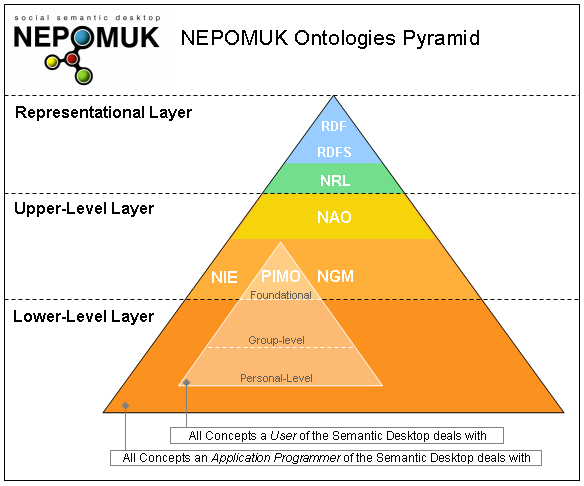
\includegraphics[width=1.00\textwidth]{images/roadmap.png}
	\caption{Integrated Ontologies}
	\label{fig:roadmap}
\end{figure}

The NEPOMUK Representational Language \textbf{NRL ontology}\footnote{\url{http://www.semanticdesktop.org/ontologies/nrl/}} builds the representational layer and the semantic
metadata axioms used to express PIMO. 
NRL is a meta-language comparable to OWL or RDF/S. 
The key characteristics of NRL are (on top of RDF/S) support for named graphs
in semantic statements, a notation for contextualized inference and semantics, 
and a selection of semantic relations (inverse, transitive, reflexive).

The NEPOMUK Information Element \textbf{NIE ontology}\footnote{\url{http://www.semanticdesktop.org/ontologies/nie/}} describes desktop elements such as address book entries, documents,
e-mails, appointments, pictures, and multimedia files.
The ontology discriminates between the representation (binary files)
and the information stored therein. 
PIMO reuses the classes of NIE and suggests how to integrate
and annotate vast personal spaces of information (PSI) expressed in NIE.

Annotations and tagging are represented in the NEPOMUK Annotation \textbf{NAO ontology}.
It represents change-dates, author, and other key metadata of documents.
NIE and PIMO both extend NAO. A part of NAO is the NEPOMUK Graph Metadata \textbf{NGM ontology} to annotate named graphs.

The PIMO ontology crosses two of the layers in the ontology pyramid, data related to PIMO can be divided into three smaller layers (also visible in Figure\ref{fig:roadmap}):
\begin{itemize}
	\item \emph{Foundational PIMO}: The PIMO ontology as such, as defined in this specification and accompanying NRL serialization. This includes the classes and properties of \emph{PIMO-upper} (see Section \ref{sec:pimoupper}), which work on the \emph{Upper-Level Layer} of NEPOMUK and everything else defined in the PIMO vocabulary. PIMO-upper is the same for every Semantic Desktop user and is valid in a global context.
	\item \emph{Group-level PIMO}: Domain ontologies that are shared within a group. They can be imported by users. A description is given in Section~\ref{sec:pimomid}.
	\item \emph{Personal-level PIMO}: The classes, properties, and Things created by an individual user. Also called \emph{user-PIMO}, this layer includes the data that is only relevant in the context of one individual.
\end{itemize}

\section{Examples}
\label{sec:examples}
A scenario is used to explain the ontology elements. A fictional persona, Claudia Stern, is our example user. She is working for EX-Ample Inc., a fictional company producing ``\textbf{Ex}treme Guitar \textbf{Ampl}ifi\textbf{e}rs'', and her current task is to organize a business trip to a meeting with guitarists and bass players in Belfast.

% taken from RDFS primer
For convenience and readability, this specification uses an abbreviated form to represent URI-References. A name of the form \texttt{prefix:suffix} should be interpreted as a URI-Reference consisting of the URI-Reference associated with the prefix concatenated with the suffix.

RDF graphs are written in N3/Turtle syntax. Examples serialized as RDF appear in this typesetting:
%\note{\emph{Knud}: I find the statement (Claudia user Claudia) very confusing. What's that supposed to mean? \emph{Leo}: that was garbage, we had it in the ontology before as an alternative to isDefinedBy.}
{\small
\begin{verbatim}
claudia:Claudia a pimo:Person;
 pimo:isDefinedBy claudia:PIMO;
 nco:hasEmailAddress <mailto:claudia@example.com> .
\end{verbatim}
}

\subsection{PIMO ontology and namespaces}
The ontology described in this document has this namespace:

{\small
\begin{verbatim}
Namespace:
http://www.semanticdesktop.org/ontologies/2007/11/01/pimo#
\end{verbatim}
}

During the lifetime of the NEPOMUK project (until Dec 2008), the PIMO ontology
and the according documentation may change, but the namespace will not change.
The namespace stays fixed to keep the necessary changes
of software implementations at a minimal level.
We have adopted this practice from other projects, which have applied it successfully. Examples are the W3C's  XSD datatypes (the recommendation changed in 2007, the namespace did not) or the FOAF project.

Throughout this document these ontologies and namespaces are used, also indicating their respective versions PIMO is building on:
{\small
\begin{verbatim}
@prefix rdf:  <http://www.w3.org/1999/02/22-rdf-syntax-ns#>.
@prefix rdfs: <http://www.w3.org/2000/01/rdf-schema#>.
@prefix nrl:  <http://www.semanticdesktop.org/ontologies/2007/08/15/nrl#>.
@prefix nao:  <http://www.semanticdesktop.org/ontologies/2007/08/15/nao#>.
@prefix pimo: <http://www.semanticdesktop.org/ontologies/2007/11/01/pimo#>.
@prefix ncal: <http://ont.semanticdesktop.org/ontologies/2007/04/02/ncal#>.
@prefix nco:  <http://ont.semanticdesktop.org/ontologies/2007/03/22/nco#>.
@prefix nfo:  <http://ont.semanticdesktop.org/ontologies/2007/03/22/nfo#>.
@prefix nie:  <http://www.semanticdesktop.org/ontologies/2007/01/19/nie#>.
@prefix nmo:  <http://www.semanticdesktop.org/ontologies/2007/03/22/nmo#>.

@prefix claudia: <http://www.example.com/people/claudia#> .
\end{verbatim}
}

\section{Creating Personal Information Models}
\label{sec:creatingPIMOs}
In this section, all key elements of the ontology are presented.
The order used reflects the steps a knowledge engineer will have to take to implement this recommendation.

\subsection{The User and their Individual PIMO}
\label{sec:pimo-user}
As a prerequisite to create a PIMO and Things inside the PIMO, each user needs a \emph{personal namespace}. The namespace is used as a prefix for all URIs minted for the user. Often these are namespaces using the HTTP URI scheme, but any RDF namespace can be used. The example namespace used in this document is \texttt{http://www.example.com/people/claudia\#} and is abbreviated with ``\texttt{claudia:}''.

\note{\emph{Knud}: In general, I would write all ontology elements in a different font. E.g., \texttt{pimo:Person}
\emph{Leo}: actually, I would like to write a script that, once this is converted
to HTML, replaces all ``pimo:NAME'' with HTML links to the ontology definition 
within the namespace.
\emph{Knud, 28/12:} unfortunately, there isn't always a namespace given. For now, I changed all ontology elements to monospaced font}

Users are represented as instances of the class \texttt{pimo:Person}. For each instance, a new URI is generated and a few key facts are represented to identify the user.
After the user has been instantiated, details such as email addresses are added by using terms from the NEPOMUK contact ontology, NCO. 
%\note{Knud: What do you mean by ``as the second object''? \emph{Leo}: fixed this, its a new resource.} 
In NCO, contact information connected to people is modeled as a complex resource, not as a simple literal:
%For the sake of simplicity, we used the URL \texttt{mailto:claudia@example.com} as identifier for this nco:EmailAddress resource.
{\small
\begin{verbatim}
claudia:Claudia a pimo:Person;
 rdfs:label "Claudia Stern";
 nco:hasEmailAddress mailto:claudia@example.com.

mailto:claudia@example.com a nco:EmailAddress;
 nco:contactMediumComment "work";
 nco:emailAddress "claudia@example.com".
\end{verbatim}
}

The second entity that needs to be represented is the \emph{Personal Information Model of the User}. It is connected to the user via the \texttt{pimo:creator} relation, and the user's namespace is added.
For Claudia this is:

{\small
\begin{verbatim}
claudia:PIMO a pimo:PersonalInformationModel;
  pimo:creator claudia:Claudia;
  nao:hasDefaultNamespace "http://www.example.com/people/claudia#";
  nao:hasDefaultNamespaceAbbreviation "claudia".
\end{verbatim}
}

\texttt{pimo:PersonalInformationModel} is a sub-class of \texttt{nrl:Ontology}, allowing more metadata to be added using NRL compliant standards. More about NRL metadata is described in Section~\ref{sec:nrlgraphs}. 
We further call a this instance of \texttt{pimo:PersonalInformationModel} of an individual a \emph{user-PIMO}. Claudia's user-PIMO is \texttt{claudia:PIMO}. As an abbreviation, it is also correct to write  ``Claudia's PIMO'' instead of ``Claudia's user-PIMO''.
\note{\emph{Knud, 28/12:} I'm confused by this term PIMO-user. It sounds as if it meant ``The user of the PIMO'', but it actually means ``The PIMO of the user'' --- correct? That's potentially confusing.} 
\note{\emph{Leo, 8/1:} reduce to ``user's PIMO'' and ``Claudia's PIMO''?}

\subsection{Things}
\label{sec:thing}
The PIMO ontology defines the basic class \texttt{Thing} for mental concepts. Every information element encountered in knowledge work by a user is represented as a Thing.
\note{\emph{Knud, 28/12:} Thing is inconsistently spelled with lower- and upper-case throughout the document.}
A Thing is a unique representation of an entity of the real world within one user-PIMO. On the PSI of a user, a real world entity can be represented in multiple data sources. For example, the person ``Dirk Hagemann'' may be author of an e-mail, described in an address book entry, and stored in a accounting tool, all part of the workspace of ``Claudia''. 
One instance of \texttt{pimo:Person} is created as unique \texttt{Thing} linking to these multiple representations, such as shown in Figure~\ref{fig:thing_vs_resource}.
\note{\emph{Knud, 28/12:} Yes, this is a Thing, but it is also a pimo:Person? Potentially confusing. \emph{Leo, 8/1:} changed the wording to speak of a Person}

\begin{figure}[htbp]
	\centering
		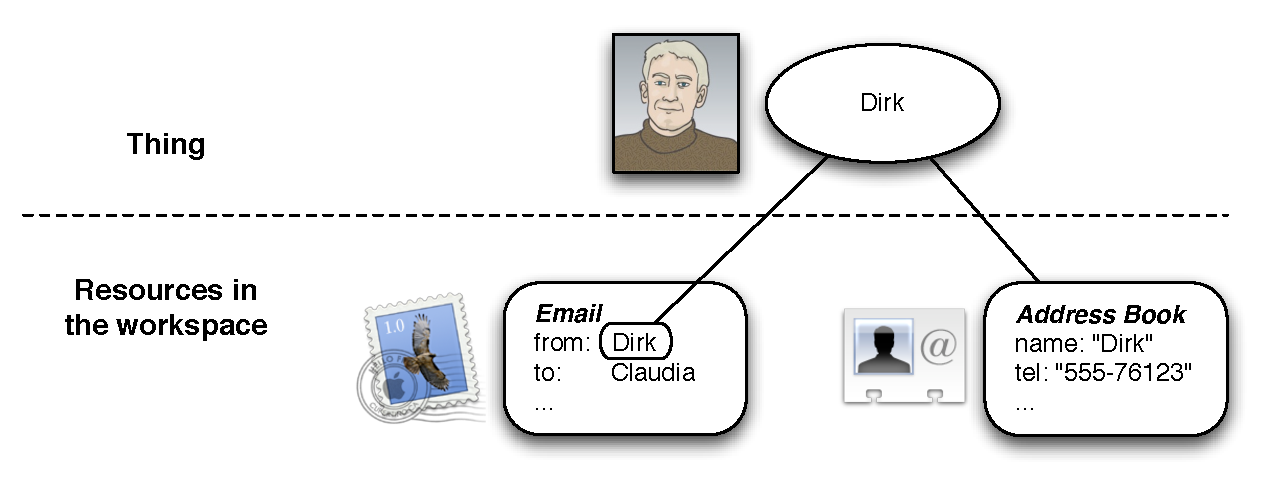
\includegraphics[width=1.00\textwidth]{images/thing_vs_resource}
	\caption{Thing and Resources}
	\label{fig:thing_vs_resource}
\end{figure}

An application handling a resource in the workspace can be aware that there may be a Thing representing the resource. For example, Claudia's e-mail client may examine the sender of an e-mail (Dirk) and search for the \texttt{pimo:Thing} that represents Dirk uniquely. Once the right Thing is found by the application, more information about Dirk can be discovered.

This principle includes all elements (\texttt{nie:InformationElement} and other RDF resources) in the user's \emph{Personal Space of Information (PSI)}. 
For each information element, a Thing in the user's PIMO must be created. 
The information element exists independent of the user, the same element can
be stored in multiple folders or data sources on one desktop, and also on other desktops and on the web. 
A Thing is the personalized view of \emph{one user} on this information element, independent of representation or storage location.

To be adequate, a PIMO of a user should contain all nameable entities known to the user,
but to be efficient, this representation should be restricted to the minimal data needed.
%Leo 29.7.2008: this is also explained later
% Identification is part of this minimal data, and \texttt{nao:identifier} provides the property for it.

\subsection{Connecting Things to the User's PIMO}
\label{sub:connectingThingsToPimo}
In a scenario of multiple connected semantic desktops, it will frequently occur that users import data from each other's desktop onto their own desktop.
It is therefore important to know which resources (primarily Things, but also Classes and Properties) were created by which user and originate from which PIMO. For this, the property \texttt{pimo:isDefinedBy} is used.

Continuing the example above, this property connects the Person to the PIMO in which it is defined.  This is mandatory for every defined Thing and allows applications to identify which elements are part of a user-PIMO and which are not\footnote{We intentionally did not only rely on NRL graphs to model the relation between the model and instances defined by it. A graph can only contain \emph{statements}, 
about, but not \emph{resources} as such.
To model that a resource is part of a PIMO, the \texttt{pimo:isDefinedBy} relation is a clear representation.
Additionally, named graphs can be used to declare what \emph{statements} are declared in a PIMO, see~\ref{sec:nrlgraphs}}.

{\small
\begin{verbatim}
claudia:Claudia pimo:isDefinedBy claudia:PIMO.
\end{verbatim}
}

An \texttt{isDefinedBy} property is also defined in RDFS, where resources can be connected to their defining ontologies, and is also discussed in the light of the OWL standard\footnote{\url{http://www.w3.org/2007/OWL/wiki/Syntax\#Declarations_and_Structural_Consistency}}. 
The semantics of \texttt{isDefinedBy} in PIMO is based on these, with the extension that we define it as a required property.

\subsection{Identification of Things}
\label{sec:identification}
A Thing \textbf{must} have an URI and \textbf{should} be described with properties that identify it. 
Identifiers allow to analyse information elements and find occurrences of the Thing.
For example, the person ``Dirk Hagemann'' is represented once as an instance of the class \texttt{pimo:Person} and identified using his e-mail address. 
The RDF descriptions of emails and documents can then be analysed to find resources that represent the same entity via this identifier. 
{\small
\begin{verbatim}
# The canonical Dirk
claudia:DirkHagemann a pimo:Person;
 pimo:isDefinedBy claudia:PIMO;
 nco:hasEmailAddress <mailto:dirk@example.com>.

# An e-mail in which Dirk #2 occurs
<imap://claudia@example.com/INBOX/1> a nmo:Mail;
 nmo:from <imap://claudia@example.com/INBOX/1#from>.

# Dirk #2, the email sender
<imap://claudia@example.com/INBOX/1#from> a nco:Contact;
 nco:hasEmailAddress <mailto:dirk@example.com>.
<mailto:dirk@example.com> a nmo:EmailAddress;
 nco:emailAddress "dirk@example.com".
 
# Dirk #3, as address book contact
<file://home/claudia/dirk.vcf#dirk> a nco:PersonContact;
 nco:nameFamily "Hagemann";
 nco:nameGiven "Dirk";
 nco:hasEmailAddress <mailto:dirk@example.com>;
 nco:photo <http://www.example.com/people/dirk/photo.jpg>.
 
\end{verbatim}
}

In this example, we see that the Person Dirk appears three times in this knowledge workspace. First, in the form of an instance of \texttt{pimo:Person}, as the canonical Dirk. Second, as sender of an e-mail and third as entry in an address book. Only one instance is the \texttt{pimo:Thing} representation of Dirk: \texttt{claudia:DirkHagemann}. The others are information elements representing the same entity.

\begin{figure}[htb]
	\centering
		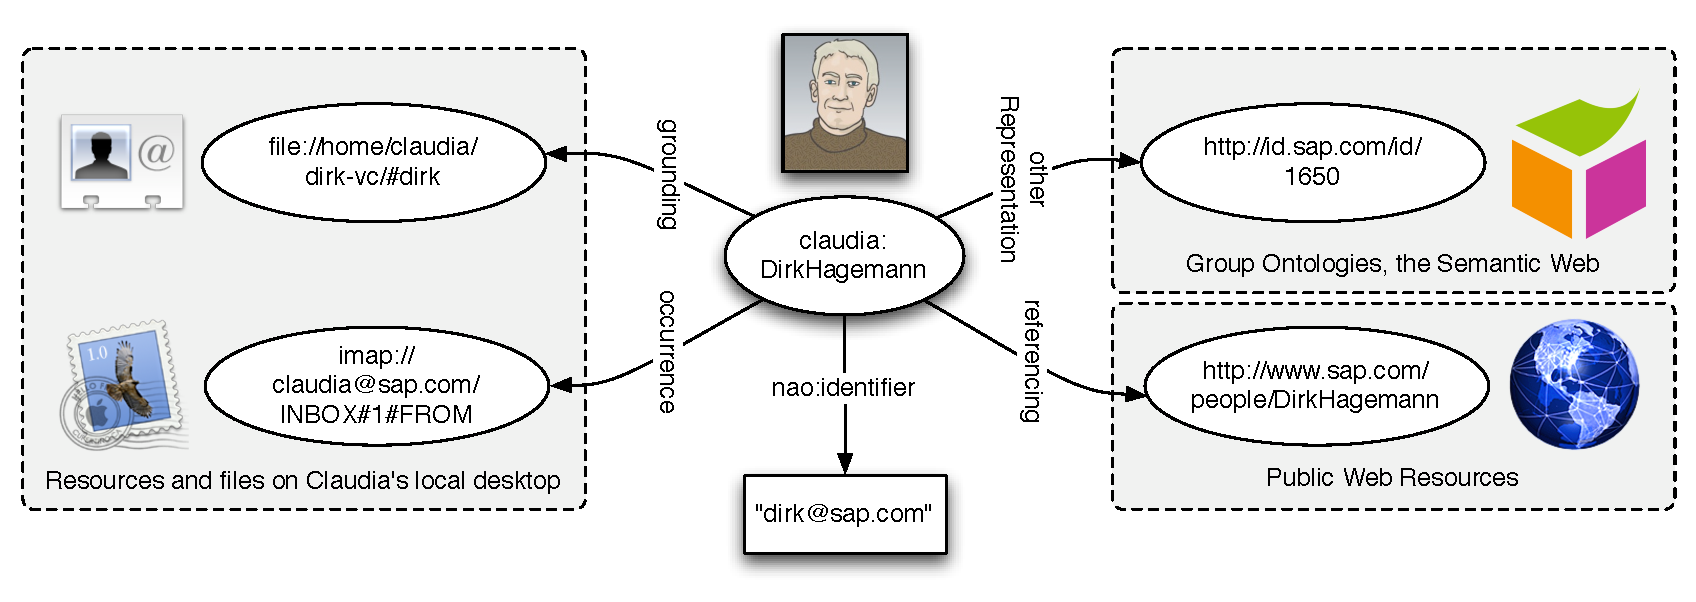
\includegraphics[width=1.00\textwidth]{images/identification}
	\caption{Different Identification Mechanisms}
	\label{fig:identification}
\end{figure}


%\note{\emph{Knud}: can one ``use'' an assumption? Leo: rephrased to ``is based on''}
To work effectively, PIMO is based on the \emph{Unique Name Assumption} (UNA). 
The UNA is a rule that declares two RDF resources with different URIs as different individuals. 
This is common in desktop applications (for example files with different names are different) and intuitive to grasp for users. But it is different from the OWL ontology language
%\note{\emph{Knud}: is OWL a system? Leo: its an ontology language}
where duplicate entries are common and the UNA is not enforced. 
PIMO is designed for personal systems, where an application has access to the complete model and can avoid duplicates before creating them.

To enforce the UNA, duplicate Things \textbf{must} be avoided. 
The crucial moment to do this is before creating a new Thing.
Things can either be created by the user manually or automatically by analysing existing native resources. In any case, before creating a new Thing, all existing Things have to be examined if a Thing with a same name or same identifying properties already exists. 
If an existing Thing is found, it \textbf{must} be reused. 
Immediately after creating a new Thing, identifying properties should be set to distinguish the Thing and avoid duplication. 
% fix to https://dev.nepomuk.semanticdesktop.org/ticket/498
Section \ref{sec:creatingthingalgorithm} further describes the complete process of creating things.

In the next paragraphs, essential identifying properties are described, an overview is given in Figure~\ref{fig:identification}.

\textbf{The primary identifier of a Thing is it's URI}. New URIs for Things \textbf{must} be generated using the namespace of the user as prefix and then a unique local name. 
Although the local name can be entirely a random string, we recommend to include the label in the URI for readability. When minting a new URI that clashes with an existing URI, a random element can be added to the new URI. A URI for Claudia Stern is:
\begin{verbatim}
claudia:Claudia
\end{verbatim}

\paragraph{NAO-Identifiers} Existing identification schemes based on NAO should be reused for this purpose by representing them with 
%\note{Knud: you say pimo:identifier here and nao:identifier in the example below. Which one is it?\emph{Leo}: its nao:identifier (28.8.2007).} 
\texttt{nao:identifier} and its sub-properties. 
If an identifier is found as meta-data of a native resource (usually an \texttt{nie:InformationElement}), the identifier \textbf{must} be copied to the Thing.
This allows others to match and identify the correct Thing when encountering the next information element.
Example identifiers are \texttt{nmo:messageId} for e-mails, \texttt{ncal:uid} for appointments, or \texttt{nexif:imageUniqueID} for images. 
Instead of using the plain \texttt{nao:identifier} property, these specific properties should be used or new sub-properties of \texttt{nao:identifier} created
\footnote{I.e. if you want to represent ISBN numbers and there is no property for them, create a new sub-property \texttt{isbn} of \texttt{nao:identifier}.}.
In this document, we assume that e-mail addresses can be used to identify persons.

\note{\emph{Leo}: this example is not good, as e-mail addresses are modeled 
differently in NCO. How else can we identify a person? \emph{Knud, 28/12:} I think we can't... :P}
\begin{verbatim}
# Copy all identifiers you can find about the Thing.
claudia:DirkHagemann a pimo:Person;
 nao:identifier "dirk@example.com".
\end{verbatim}

Identifiers consisting of multiple RDF statements cannot be captured using \texttt{nao:identifier}.
They are comparable to a primary key in a relational database consisting of multiple
columns. These \textbf{multi-key identifiers} \textbf{must} be merged into one \texttt{nao:identifier}.

\paragraph{Grounding Occurrence} The relation \texttt{pimo:groundingOccurrence} is used to link a Thing to an \texttt{nie:InformationElement} that has this Thing as primary topic. For example, the grounding for a person could be the entry in the address book describing the person. On the other hand, an e-mail with this person as the sender or recipient would normally not be a grounding occurrence. A Thing represents the mental concept, the \texttt{pimo:groundingOccurrence} links to existing Information Elements that are handled by existing applications. This is a key for reusing the features of these applications. 
The grounding occurrence can change, for instance if a file was moved and the URI of the Information Element changed, the grounding occurrence relation needs to be changed. 
A similar case happens when a file is uploaded to a shared workspace and not kept locally any more --- all annotations of the Thing stay the same (the URI of the Thing does not change), the Information Element changes.
Multiple values are allowed, this reflects the fact that the same Thing can be represented in multiple applications, and dependent on the work context, the user may want to open a different application. 
{\small
\begin{verbatim}
# Link to Dirk #3 from example above.
claudia:DirkHagemann a pimo:Person;
 pimo:groundingOccurrence <file://home/claudia/dirk.vcf#dirk>.
\end{verbatim}
}
\paragraph{Occurrence} The relation \texttt{pimo:occurrence} connects a \texttt{pimo:Thing} with a resource representing the same real world entity.
Facts about the occurrence are then also valid for the connected Thing. 
For example, if the person Dirk appears as sender of an e-mail, then the resource identifying the sender is an \emph{occurrence} of Dirk. 
Based on the occurrence relation, Dirk (the unique \texttt{pimo:Person}) is the sender of the given e-mail.
Occurrence relations are to be used on resources \emph{representing} the same entity in a different context, but not on resources \emph{mentioning} the entity. For example, it is not valid to say that an e-mail is an occurrence of a person, only the sender or recipient can be occurrences of a person.

%Not the e-mail as such is the occurrence, but the sender within. 
\note{\emph{Knud, 28/12:} Why is the e-mail as such not the occurrence? This should be explained, or not mentioned at all. 
Leo: done, removed sentence, replaced with longer explanation.}
Occurrences of a Thing can be found by searching for entities with the same identifying properties.

{\small
\begin{verbatim}
# Link to Dirk #2 from example above, 
# he occurs as sender of an e-mail
claudia:DirkHagemann a pimo:Person;
 pimo:occurrence <imap://claudia@example.com/INBOX/1#from>.
\end{verbatim}
}

Besides identification, both the \texttt{pimo:groundingOccurrence} and the \texttt{pimo:occurrence} relation have 
implications on data integration and affect semantic meaning of a Thing. 
This will be described later in Section \ref{sec:pimoVSnie}.

\paragraph{Referencing Occurrence} 
%\note{Maybe rename to indicatingOccurrence, closer to Topic Maps? Leo: I don't care, leave it as is.}
\label{par:referencingOccurrence}
A Referencing Occurrence is an indirect approach to identification. 
Annotating a Thing with an information element as \emph{referencing occurrence} states that the information element contains a description of the Thing.
Its primary topic must be the Thing.
The Thing is indirectly identified by the element, when two Things in different models share the same information element as referencing occurrence, they may be equal and could be matched. 
The following description is an adaption of XTM's subject indicators~\cite{XTM,Rath2003}.
The referencing occurrence is a kind of proxy for the Thing. Examples of referencing occurrences are:

{\small
\begin{verbatim}
claudia:DirkHagemann a pimo:Person;
 pimo:referencingOccurrence <http://www.example.com/people/DirkHagemann>.
 
claudia:ExampleInc a pimo:Organization;
 pimo:referencingOccurrence <http://www.example.com/>;
 pimo:referencingOccurrence <http://en.wikipedia.org/wiki/Example.com>.
\end{verbatim}
}

It should contain a human readable documentation describing the concept. The resource could be a document, ontology, video, audio, anything able to describe to a human what the concept is about. The resource is a reference to the concept of the Thing. 
A good example for a referencing occurrence is a wikipedia article.

A referencing occurrence describes the concept with the purpose of being widely used by ontologies. Consequently, it is important that the document describes exactly what concept it is about and what not. Even if the author works as accurately as possible, different people will never interpret a referencing occurrence 100\% the same way. However, the concept of referencing occurrences is worth using it, because it allows a shallow match of heterogenous information models, and because there is finally no alternative to it. 

\textbf{It is recommended to use wikipedia URIs as objects of referencing occurrences.} In contrast, URIs minted by \emph{DBPedia}\footnote{DBPedia is a Semantic Web representation of wikipedia and provides URIs for concepts, whereas wikipedia provides URIs for documents describing concepts. An example DBPedia URI is: \url{http://dbpedia.org/page/Berlin}} \textbf{must} be related using the \texttt{pimo:hasOtherRepresentation} relation.

\paragraph{Other Representation} 
\label{par:otherRepresentation}
The \texttt{pimo:hasOtherRepresentation} relation is used to connect \texttt{pimo:Things} with other representations of the same Thing in other Semantic Web ontologies. 
This can be the case with shared ontologies, such as company white page systems or Semantic Social Networking websites. 

The knowledge modeled should be compatible with the ontologies used by the user. An example for such other representation is\footnote{Using the URI scheme of the ECS University in our example domain. \url{http://id.ecs.soton.ac.uk/docs/}}:
\begin{verbatim}
claudia:DirkHagemann a pimo:Person;
 pimo:hasOtherRepresentation <http://id.example.com/person/1650>.
\end{verbatim}

Another example would be the city of Belfast where Claudia wants to travel to,
linked to the DBPedia entry about it:
\begin{verbatim}
claudia:Belfast a pimo:City, pimo:Tag;
  pimo:isDefinedBy claudia:PIMO;
  pimo:tagLabel "Belfast";
  pimo:hasOtherRepresentation <http://dbpedia.org/resource/Belfast>;
  geo:lat "54.5833333";
  geo:long "-5.9333333".
\end{verbatim}
The relation can be used both to identify Things by their other representations,
and to fetch more data.
In this example, the latitude and longitude are actually superfluous data,
as they can be retrieved from the other representation
in DBPedia.
Assuming Dirk also represents Belfast in his PIMO, but independent from Claudia,
but linking to the same DBPedia entry, algorithmically matching their different representations is straightforward.

\paragraph{Other Conceptualization}
To map user-generated classes to classes defined in other ontologies, the 
\texttt{pimo:hasOtherConceptualization} relation connects classes defined in a user's PIMO
with classes defined in domain ontologies. 
Classes defined in domain ontologies should be sub-classes of PIMO-upper classes, see Section \ref{sec:integratingontologies}. 

Implementations can use the \texttt{pimo:hasOtherConceptualization} to allow the user and algorithms
to map user--specific classes to classes defined in other ontologies,
without implying that there is a sub-class relationship.

\subsection{A Complete Example} 
A complete example for all different identification properties 
can now be built from the above annotations.

For Claudia, her co-worker Dirk Hagemann is identified and linked to occurrences like this:

{\small
\begin{verbatim}
# The canonical pimo:Person Dirk, 
# a pimo:Thing from Claudia's PIMO
claudia:DirkHagemann a pimo:Person;
 pimo:isDefinedBy claudia:PIMO;
 nao:prefLabel 'Dirk Hagemann';
 nao:identifier "dirk@example.com";
 pimo:occurrence <imap://claudia@example.com/INBOX/1#from>;
 pimo:groundingOccurrence <file://home/claudia/dirk.vcf#dirk>;
 pimo:referencingOccurrence <http://www.example.com/people/DirkHagemann>;
 pimo:hasOtherRepresentation <http://id.example.com/person/1650>.
 
 
# An e-mail in which Dirk #2 occurs
<imap://claudia@example.com/INBOX/1> a nmo:Mail;
 nmo:from <imap://claudia@example.com/INBOX/1#from>.

# Dirk #2, as email sender
<imap://claudia@example.com/INBOX/1#from> a nco:Contact;
 nco:hasEmailAddress <mailto:dirk@example.com>.
 
<mailto:dirk@example.com> a nmo:EmailAddress;
 nco:emailAddress "dirk@example.com".
 
# Dirk #3, as address book contact
<file://home/claudia/dirk.vcf#dirk> a nco:PersonContact;
 nco:nameFamily "Hagemann";
 nco:nameGiven "Dirk";
 nco:hasEmailAddress <mailto:dirk@example.com>;
 nco:photo <http://www.example.com/people/dirk/photo.jpg>.
\end{verbatim}
}

This allows implementations to:
\begin{itemize}
	\item identify the Thing when found occurring in documents,
	\item open a grounding occurrence to see the Thing within an existing desktop application (i.e. the address book entry for a person),
	\item match this Thing with other representations via the same referencing occurrence,
	\item use the other representation from the company's white pages to show additional data about the Thing.
\end{itemize}

The \texttt{pimo:occurrence} link is the generic basis, \texttt{pimo:groundingOccurrence} and \texttt{pimo:hasOtherRepresentation} are sub-properties of it. This data should be generated automatically and unsupervised. 
Adding identifying properties to a Thing helps to find more occurrences and therefore more information about it.

\subsection{Labels and Names of Things}
\label{sec:labelling}
To label Things, we recommend the NEPOMUK Annotation Ontology (NAO) vocabulary
and extended it.
NAO defines properties for the \emph{preferred label}, \emph{multiple alternative labels}. PIMO defines \emph{tag labels} as unique names for unique Tags.

\paragraph{\texttt{nao:prefLabel}} \textit{A preferred label for a Thing}.
This property \textbf{must} be applied to every instance of \texttt{pimo:Thing} (or its sub-propery \texttt{pimo:tagLabel}).
It can be used by applications to represent the Thing with a textual label and should be human-readable. There must only be one \texttt{prefLabel} per Thing (mincardinality and maxcardinality should be one)\footnote{These restrictions are not explicitly noted in the RDF description of the property, as NRL does not support property restrictions for classes.}.

\paragraph{\texttt{pimo:tagLabel}} \textit{Defines a unique personal label for a Thing, which then is also a Tag.}
The label \textbf{must} be unique within
the scope of a user. 
If both are set, \texttt{pimo:tagLabel} and \texttt{nao:prefLabel} of a resource \textbf{must} have the same value. 
It is a sub-property of \texttt{nao:prefLabel} and of \texttt{nao:personalIdentifier}.

\textbf{Tag labels are the \textbf{recommended} way to label and identify Things that are used for classification}.
As they are unique and human-readable, they \textbf{may} be used for multiple application scenarios such as wikis, tagging, or matching terms found in free-text.
Naming a Thing with a \texttt{pimo:tagLabel} gives the Thing a second type, \texttt{pimo:Tag}, which indicates that the Thing should now be considered part of the user's tagging system, see Section~\ref{sec:tagginginpimo}. 
\note{\emph{Knud, 28/12:} I don't understand: should the two properties be the same or not? Leo: recommended they should be the same.}

\paragraph{\texttt{nao:altLabel}} \textit{An alternative label alongside the preferred label for a Thing.} These are alternative spellings, translations, nick-names.
%\note{\emph{Knud, 28/12:} Spelling Mistakes? Leo: removed this, replaced with nick-names}
Implementations can use these labels to find Things when the user enters a text in a search box or when analysing free text.
If a Thing has occurrences, the labels of occurrences \textbf{should} be copied as alternative labels to the thing.

In combination, these labelling techniques allow applications to clearly label Things in user interfaces but also to lookup for Things based on alternative names. For our example, these are:

\begin{verbatim}
claudia:DirkHagemann a pimo:Person;
# preferred label when shown
 nao:prefLabel "Dirk Hagemann";
# a nickname for Dirk
 nao:altLabel "hacki";
# a common misspelling
 nao:altLabel "Dirck Hagemann";
# the personal identifier and tag label, 
# Attention: this requires the class pimo:Tag
 pimo:tagLabel "Dirk Hagemann".
\end{verbatim}

Additionally, visual cues (icons, images, thumbnails) can be attached by using NAO symbol relations:
\begin{itemize}
	\item \texttt{nao:hasSymbol}
	\item \texttt{nao:prefSymbol}
	\item \texttt{nao:altSymbol}
\end{itemize}

\subsection{Textual description of Things}
\label{sec:freetextdescription}
To describe Things with a free-text, the simple \texttt{nao:description} property should be used. This allows users to add a (possibly searchable) description of the Thing in a simple way. The description string value should contain no format markup but be a plain text.

For more complex free-text descriptions of Things, the property \texttt{pimo:wikiText} is reserved. 
Formatting (font-weight, italics) and linking to other pages is supported
in this property, implementers may use the \emph{Wiki Interchange Format}
\footnote{\url{http://semanticweb.org/wiki/Wiki_Interchange_Format}}
as syntax, or RDFa\cite{rdfaprimer}.

\subsection{Rating and Ranking Things} % (fold)
\label{sec:ratings}
\textbf{Ratings of Things} can be expressed using \texttt{nao:numericRating}.
For numericRating, the range of values \textbf{must} be within $[0..10]$ (inclusive)
\footnote{Implementers may wonder why the range is not standardized as $[0..1.0]$. The recommended range is based on an implementation decision taken in KDE.}. 
A value of '0' is interpreted as not set, a rating of 1 a \emph{bad rating} and a rating of 10 a \emph{good rating}. 
Furthermore, resources can only be given at most one numeric rating, thus the maximum cardinality is 1.
Applications \textbf{may} partition the values into discrete ratings (such as 2, 4, 6, 8, 10 to represent the semantics of ``5 star ratings'').

The rating values may and should be used for \emph{ranking} of Things
and filtering. A populated PIMO contains thousands of Things,
user interfaces should use the \texttt{nao:numericRating} values
to filter out low-ranked resources and highlight high-ranked
resources.
Implementations \emph{can} set the \texttt{nao:numericRating} 
values automatically to computed values.
% Alternatively, implementations can set an automated rank and
% compute the overall rank using auotmated rank + nao:numericRating


% paragraph ratings (end)

\subsection{Modelling Time}
In PIMO, no special treatment of time is modeled. 
We are aware that representing points in time, durations, and other periods of time
is an important aspect of ontologies. 
We recommend to use the XML Schema Datatypes
to represent time. 
There, ISO 8601 is recommended. Timezones must be handled according to this standard,
encoded inside the literal value\footnote{For a detailed representation of time events, refer to the NIE documentation, where timezones are discussed (\url{http://www.semanticdesktop.org/ontologies/2007/04/02/ncal/\#sec-tzd}).
NIE represents time using the NcalDateTime class and its properties 
date, dateTime, ncalTimezone. Timezones are represented using a Timezone class,
that is inspired by RFC 2445.}.

Periods of time can be represented using sub-classes of the abstract class
\texttt{pimo:ProcessConcept} which represents lasting processes such as events
or projects. For durations that last a number of days or months, we recommend to use the standardized XML datatypes\footnote{The XS namespace is \texttt{http://www.w3.org/2001/XMLSchema}, but the two duration datatypes are defined in the XPath recommendation in 2007, see \url{http://www.w3.org/TR/xpath-functions/\#dt-dayTimeDuration}}:
\begin{itemize}
	\item \texttt{xs:dayTimeDuration} for durations measured in days, hours, and minutes.
	\item \texttt{xs:yearMonthDuration} for durations measured in months and years
\end{itemize}
Implementers are free to use either the XSD types or sub-classes of 
\texttt{pimo:ProcessConcept}.

There have been issues with other notations of duration and therefore the W3C Semantic Web Best Practices and Deployment Group published a note\footnote{\url{http://www.w3.org/TR/swbp-xsch-datatypes/\#section-duration} Since XPath 2.0 has become a W3C recommendation in January 2007, this note is partly obsoleted.} to restrict durations to these values. 

\subsection{Representing Modification and Change Dates}
\label{sec:changedates}
The change and creation dates of Things are important metadata for personal information management applications. Knowing about recent changes is an important cue for users to retrieve documents. Many applications offer the feature to show recent changes or filter by them. Consequently, it has to be straightforward, simple, and fast to query for the modification dates. 

The NAO properties \texttt{nao:created}, \texttt{nao:modified}, and \texttt{nao:lastModified} \textbf{shall} be used to track the change dates of Things. 
Creation and modification allow only one, modification allows multiple date values.
Created and lastModified values \textbf{must} be set for each Thing,
at least one modified value \textbf{must} be set.
These values are intended for resources of type \texttt{pimo:Thing}, \texttt{pimo:Association}, \texttt{rdfs:Class}, and \texttt{rdf:Property} when created by the user.
\note{\emph{Knud, 28/12:} Why is this not enforced? 
\emph{Leo, 8/1:} mandatory is better anyway, CHANGED}

Example:
\begin{verbatim}
# Represent modification dates of a Thing
claudia:DirkHagemann
  nao:created "2007-10-26T15:23:01";
  nao:modified "2007-10-26T15:23:01";
  nao:modified "2007-10-29T08:04:30";
  nao:lastModified "2007-10-29T08:04:30".
\end{verbatim}

The \textbf{semantics} of these dates is that the description of the Thing has changed, facts about the Thing have been added, removed, or modified. Changes to \texttt{pimo:objectProperty} (\texttt{pimo:related}, \texttt{pimo:hasTag}, etc.) or \texttt{pimo:datatypeProperty}  (\texttt{name}, \texttt{address}, \texttt{label}, etc.) imply such a modification. 
Included are also changes to the labels (\texttt{nao:prefLabel}, \texttt{nao:altLabel}, \texttt{pimo:tagLabel}).
Modification of any other statement (such as \texttt{pimo:definedBy}, \texttt{nao:modified}) do not imply a modification nor a change of dates.
As current RDF stores a priori do not support automatic tracking of changes, applications have to implement housekeeping of these dates, or use services for tracking.
\footnote{The value of lastModified is redundant as it could be computed by sorting the modified dates during query time, but this is not possible without nested SPARQL queries, a $max()$ function, and grouping, none of these part of the SPARQL standard. The stores that support such non-standard operations still need time to compute the value. As the last modification date is very important for applications to assist users finding information, the redundancy is intended.}

\note{\emph{Knud, 28/12:} I removed a paragraph here (still commented in the source), because I think it doesn't belong here. This document is a specification, not a scientific document. Leo: OK}
%In RDF and using named graphs, there are more ways of representing change dates. It is possible to remember the date when a graph changes, implying that all triples inside the graph have changed. Based on this, it can be implied that all resources described in these triples have changed. But there is no formal relation between a resource and a graph that describes it. For example a class being used as object of a rdf:type relation, does this express that the class has changed? Or a resource being annotated in a reification statement. Changes to the graph may not directly relate to changes of the resource in the view of the user. 
%Also, as dates are a very prominent fact needed for data visualization and search result ranking, a graph-based approach will not provide satisfactory answer times
%\footnote{To select a date using graph metadata, a query for the context of all statements where a resource is either in subject or object role and the change date of these contexts would be needed.}.

\subsection{Setting the Class of a Thing}
\label{sec:classofthing}
All Things are of type \texttt{pimo:Thing} or one of its sub-classes. The PIMO ontology itself defines several sub-classes such as \texttt{pimo:Person} or \texttt{pimo:Organization}. If these are not specific enough, the user can either create new sub-classes manually (see Section \ref{sec:customontology}), or import group-level ontologies (Section~\ref{sec:integratingontologies}).

As a rule of thumb, the question to be answered by assigning the class is ``\emph{What is this Thing?}''.
In comparison to OWL, where classes are commonly based on the properties of the object (``vegetarians are entities not eating flesh'') , classes represent the type (the \emph{nature}) alone. 
\note{\emph{Knud, 28/12:} idea: paragraphs such as this should be marked as ``suggestion for use''. Again, they don't really belong in a specification.
\emph{Leo, 8/1:} This paragraph is explanatory of the idea of classes in comparison to OWL, where most things are modeled as ``does this thing belong to a class or not'' Its important to have it. Cutted it, reworded it to refer to OWL. DONE?}
%For the concrete example of ``importance'', we recommend using the property \texttt{nao:numericRating} or by using part-of relations like ``this Thing is part of the collection of important things''.
%To model collections of things that share a common property (such as ``important Things''), the class \texttt{pimo:Collection} is provided.

It is also recommended to only use one explicit class for a Thing. The wish to add multiple classes is often an indication that some classes can be better modeled using relations. 
For example, it is recommended to use a datatype property \emph{``is this person a vegetarian? yes or no''} and explicitly set it instead of assigning a sub-class of Person called \emph{Vegetarian}.
If Things with two classes are needed (for example, if something is both a ``Car'' and a ``Locatable'') then the preferred way is to change the class model (make Car a subclass of Locatable or create a new class ``LocatableCar'' with both as superclass) than to add both types to one Thing. Nevertheless, it is not forbidden to add two types.
%Superclasses are inferred implicitly, and are not affected by this recommendation.

When a Thing has occurrences that are expressed in the NEPOMUK Information Element ontology (NIE), suitable mappings from NIE classes to PIMO classes are available in a mapping file
\footnote{\url{http://www.semanticdesktop.org/ontologies/2007/11/01/nietopimomapping.rdf}}.

\subsection{The PIMO-upper ontology}
\label{sec:pimoupper}
PIMO contains an \emph{upper ontology} for basic concepts in Personal Information Management (PIM):
Person, Location, Event, Organization, Topic, Document, Time. They are modeled
to answer basic questions about a Thing:
\begin{itemize}
	\item Who is associated? Person
	\item Where is this? Location
	\item When is it? Time
	\item What is it about? Topic
\end{itemize}
% addressing the ``foundational'' part of figure 1
The classes are the \emph{foundational part} of PIMO in the \emph{Upper-Level Layer} of the overall NEPOMUK ontologies as shown in~\ref{fig:roadmap}.
This level serves as integration point for PIM applications,
in the broader perspective of the Semantic Desktop, the classes can serve as upper classes for group-- and domain--level ontologies (see Sect.~\ref{sec:integratingontologies}).

\subsection{Classes in PIMO-Upper}
\label{sec:pimoUpperClasses}
The classes have been defined based on related ontologies, a user study, and several software prototypes that have been evaluated. Figure~\ref{fig:upperclasses} gives a rough overview of the available classes.

\begin{figure}
	\centering
		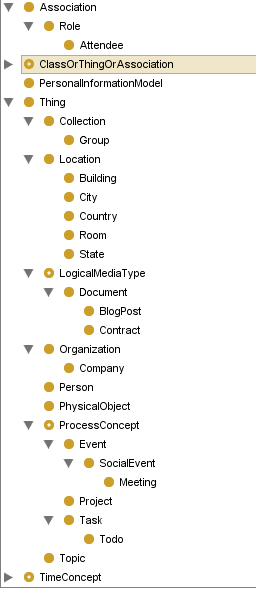
\includegraphics{images/upperclasses.png}
		\caption{Classes in PIMO-Upper}
	\label{fig:upperclasses}
\end{figure}

\begin{description}
%
%    NOTE !!!!!!!!!!!!!!!!!!!!!!!!!!!!!!!
%    These are copied from the ontology, and if not, the
%    descriptions have to be the same in the ontology and here.
%
	\item[Thing] The root class of the upper ontology. Every entity that can be in the direct attention of the user is a Thing.
	\item[Collection] A collection of Things, independent of their class. The items in the collection share a common property. Several usability studies showed that collections are important for PIM. It is recommended to either use the \texttt{pimo:hasPart} or the \texttt{pimo:isTagFor} relation to connect a collection with the Thing it contains\footnote{A Risk Of Change: A clear recommendation to either property may follow in future versions}.
	\item[Group] A group of Persons. They are connected to each other by sharing a common attribute, for example they all belong to the same organization or have a common interest.
	\item [Location] A physical location. Sub-classes are modeled for the most common locations humans work in: Building, City, Country, Room, State. This selection is intended to be applicable cross-cultural and cross-domain. City is a prototype that can be further refined for villages, etc.
	\item [LogicalMediaType] MediaConcepts are logical media types (e.g., a book, a contract, a promotional video, a todo list).  The user can create new logical media types dependent on their domain: a salesman will need MarketingFlyer, Offer, Invoice while a student might create Report, Thesis and Homework.
	\item [Organization] An administrative and functional structure (such as a business or a political party).
	\item [Person] Represents a person. Either living, dead, real or imaginary. In this regards, similar to \texttt{foaf:Person}.
	%\item [PhysicalObject] An object of interest in the physical world. \note{\emph{Knud}: if there is a physical object, how about an abstract object? Love? Language?
%\emph{Leo}: correct. I see a problem with Organozations and Topics, they have
%an overlap with AbstractObject. This can lead to a longer discussion...
%	we should consult sumo. I added this as an open issue at the end.\ref{issue:abstractobject}}	
%	It can be touched, it is concrete and it is of interest to the user. Examples are cars, tables, products and goods of business interest.
	\item[ProcessConcept] Concepts that relate to a series of actions or operations conducing to an end. Sub-classes are defined for Event, SocialEvent, Meeting, Project, and Task.
	\item[Topic] A topic is the subject of a discussion or document. Topics are distinguished from Things in their taxonomic nature, examples are scientific areas.
	\item[Tag] Tag is an abstract marker class to specify which Things in the user's PIMO should be considered useful tags in a tagging system. All Topics are Tags (Topic is a subclass of Tag). Implementations should support the user by using a useful set of Things as Tags, see Section~\ref{sec:tagginginpimo}.
\end{description}

These classes are intentionally kept generic. More specialized ontologies should be used for certain domains of application, see Section~\ref{sec:integratingontologies}. The classes of these ontologies are then  sub-classes of upper ontology classes. 

\subsection{Describing Things with Attributes and Relations}
\label{sec:describingthings}
Conventional RDF statements are used to describe Things. Predicates have to be defined as \texttt{rdfs:Properties} according to the NRL standard. Alternatively, it is also possible to use properties from other modeling languages like OWL or RDFS although we do not encourage this without a proper mapping of existing ontologies to PIMO (see~\ref{sec:integratingontologies}).

Properties that are intended to be editable and visible to end users \textbf{must} be sub-properties of either \texttt{pimo:datatypeProperty} or \texttt{pimo:objectProperty}.

Many NIE and NAO properties can be used from PIMO Things, see Section~\ref{sec:usingnieinpimo}. 

\subsection{Generic Properties in PIMO-Upper}
\label{sec:genericproperties}
The PIMO-upper ontology contains basic relations between Things and a few core attributes for identifying them (described above in Sect.~\ref{sec:identification}). 
These sub-properties of \texttt{pimo:objectProperty} are:
\begin{description}
  \item [\texttt{pimo:related}] is the most generic relation, giving no further indication how Things may be related. Related is defined to have itself as inverse property, 
  it is indirectly a \texttt{nrl:SymmetricProperty}, but does not inherit this attribute to sub-properties. Sub-properties can be asymmetric, depending on the inverse-of relation they define.
	\item [\texttt{pimo:hasPart}] and \texttt{pimo:partOf} model partitive relations. They are inverse. Neither is transitive, because part-of relations used for modelling in the domain of Personal Information Management are vague due to the many contexts of interpretation (a hotel may be part of a trip plan, a trip plan part of a project, but this does not indicate the hotel to be part of the project).
	\item [\texttt{pimo:hasTag}] and \texttt{pimo:isTagFor} connect a Thing of interest with a Tag characterizing it. For example, a meeting can have a project as a tag, or a document has a meeting as a tag, when the goal of the meeting is to discuss the document. After the meeting, the meeting minutes are a new Thing having the meeting as a tag. This is not restricted to meetings but also an organization or a person can have a certain technology as a tag to express that they are working on the topic described by the tag. The relation is not transitive, not symmetric. It is not asymmetric because a thing A may have thing B as tag, and B also A, if both are tags. The range of the \texttt{pimo:hasTag} relation is restricted to the class \texttt{pimo:Tag}. Topic is a subclass of tag. See Section~\ref{sec:tagginginpimo}.
\end{description}

Implementers may use these generic properties directly, or create sub-properties of them
or sub-properties of the more generic \texttt{pimo:objectProperty}.
The main reason to have the generic properties is the semantic meaning of the relations,
which can help to create user interfaces or model domains. 
Ontology authors can ask themselves ``does a new property model a part-of relation or not, does it assign a thing with a topic, or is it a generic relation?'' and then extend one of the generic properties.

For these generic relations, specialized sub-properties are defined when used on specific  classes in the PIMO upper ontology.

\subsection{Refined properties in PIMO-Upper}
\label{sec:pimoupperrelations}
Additional to the above relations, semantically interesting relations between PIMO upper classes are modeled. Especially those which can be used as symmetric or transitive relations for inference.

\begin{description}
	\item[\texttt{pimo:subTopic}] and \texttt{pimo:superTopic} relate Topics to each other. As Topics are an important mean to organize document collections based on a taxonomy, these two predicates are defined. They are inverse of each other and transitive.
	\item[\texttt{pimo:hasOrganizationMember}] and \texttt{pimo:isOrganizationMemberOf} are relations connecting a Person to an Organization.
	\item[\texttt{pimo:hasLocation}] and \texttt{pimo:isLocationOf} relate a locatable Thing with its Location. Locatable is an abstract sub-class of Thing.
	\item[\texttt{pimo:containsLocation}] and \texttt{pimo:locatedWithin} relate two locations within each other. Note that for geographic locations representing a physical space, inclusion is transitive.
\end{description}

\subsection{Tagging Things with Tags}
\label{sec:tagginginpimo}
% Say that PIMO is intended to work as an ontology, but also as a tagging system. When tagging e-mails or other elements, the name of the used tag must be unique. This is to be compatible with existing tagging systems, and to simplify the model. Intended use of TAG is to build a tag-cloud and organization system for the user's documents. Say that all topics are tags and are also arranged in a hierarchy (see next section). Recommend which classes make good tags: classes that exist for a longer time and can be used to classify many documents: topic, collection, group, city, person, organization, project. Say why it won't work without pimo:Tag. The classification system must be smaller than the document collection, to optimize retrieval.
The generic properties described in the last Sections show how Things can be related to each other.
An important aspect of PIMO is to classify Things using ``Tags''. 
Compared to normal PIMO Things, \emph{Tags} have one important additional restriction to make them compatible with Tags from other tagging system (folksonomies and Topic Maps):
\begin{itemize}
	\item The label of a Tag is unique, within the scope of one Personal Information Model.
\end{itemize}
Using Tags, PIMO can be used similar to an existing tagging system.

To extend a Thing to become a Tag, add the type \texttt{pimo:Tag}:
\begin{verbatim}
# The Person Dirk
claudia:DirkHagemann
  a pimo:Person;
# also a Tag
  a pimo:Tag;
# Must define the required pimo:tagLabel
  pimo:tagLabel "Dirk Hagemann".
\end{verbatim}
The \texttt{pimo:tagLabel} is required for all instances of \texttt{pimo:Tag}, and as it is a subproperty of \texttt{nao:prefLabel}, it can replace an existing prefLabel.
The \emph{intended use of Tags} is to build a clear category system for the user's documents. 
Once a Thing is \emph{tagged}, it can be retrieved by finding first the Tag, and then Things associated with the Tag.
A user's Tags are good candidates as first entry points to explore a data space, they can be visualized in a tag cloud or an alphabetical list. Tags can be clustered by type (each has an additional PIMO type), and by hierarchy (Tags can be organized in a part-of hierarchy, Topics are organized in a subTopic hierarchy).

To be useful as classification system, there should be a limited number of Tags to classify the potentially larger amount of documents. 
Examples are Things which exist for a longer period of time and Things that are of much importance to the user. 
Implementations \textbf{should} provide means to use the following as Tags.
\begin{itemize}
	\item All \textbf{Topics} can be considered Tags. This is expressed by the fact that Topic is a subclass of Tag.
	\item \textbf{Collections} work well as Tags, the act of putting something into a collection can be considered an act of tagging.
	\item A \textbf{person}.
	\item A \textbf{group of persons}. 
	\item A \textbf{city}, as there is a limited number of cities a person interacts with. 
	\item \textbf{Projects} are defined as an ``enterprise carefully planned'', the planning and execution of a project may involve tagging many Things as belonging to the project.
	\item A \textbf{task}, as documents may be needed to fulfill the task.
	\item An \textbf{organization} to classify to which organization a person belongs or by which organization a document was published.
\end{itemize}
The process of using an existing Thing as Tag \textbf{may} be automated. For example, a user searching for a possible Tag for a document should be able to pick from a list of existing Tags, and additionally search for Things of the above type to convert them to a Tag (such as a ``more Tags'' button). 
The conversion from Thing to Tag \textbf{may} then be automated and not visible to the user.

Tagging a document is illustrated in the following example, for more details refer to Section~\ref{sec:taggingfiles}.
\begin{verbatim}
claudia:BelfastMeetingPackage a claudia:MeetingPackage, pimo:Tag;
  pimo:tagLabel "Belfast Meeting Package".

claudia:BelfastBusTimetable a pimo:Document;
  pimo:groundingOccurrence <file://home/claudia/doc/tripplan.pdf>;
  pimo:hasTag claudia:BelfastMeetingPackage.
\end{verbatim}

In general, it should be avoided to use \texttt{pimo:Document} instances as Tags.
Typically the amount of documents is high, making them less useful as categorization scheme compared to the above mentioned Thing classes. 
The reason to introduce Tags in PIMO is to allow implementers to separate between categorization scheme and annotated instance base (which is usually a document corpus).
Without a class to mark Tags, it would not be possible to restrict the \texttt{pimo:tagLabel} predicate to a minimum cardinality of one, and also Topics could not automatically be defined as Tags.

\subsection{Topic Hierarchies}
\label{sec:topichierarchies}
% say that PIMO is a taxonomy system comparable to SKOS. The hierarchical ordering of Topics is important to organize the system. Hierarchies are also used to allow semantic search on subtopic structures. add rules.
The methodologies so far allow the description of individual Things with labels, properties, classes, and Tags. 
Besides the view on individuals, their place inside an overall organization scheme of the user can be important --- where is a Thing located in a hierarchy? 
Things can be placed in a hierarchy using the \texttt{pimo:hasPart} relation. 
In an overall hierarchy, the part relation can be confusing, as Things both have a class and can be part of something. For example, \emph{workpackage 2} is \emph{part of } the \emph{CID project}. In a combined hierarchy including class and part-of relations, it would appear at two positions: as instance of workpackage and as part of CID. 

To simplify the system for novice users, it is \textbf{recommended} for implementers to support a \emph{Topic Hierarchy}, where hierarchical part-of structures are shown to end-users. The semantic ``is-a'' relations \textbf{should} be hidden in the Topic hierarchy.
This allows users to model parts of their PIMO as taxonomy.
\begin{itemize}
	\item Each instance of \texttt{pimo:Topic} \textbf{must} either have a \texttt{pimo:hasSuperTopic} relation to another Topic or be defined as root Topic using \texttt{pimo:hasRootTopic}.
	\item All Topics \textbf{must} be connected (indirectly or directly) to a root Topic, or be a root Topic themselves.
	\item User interfaces \textbf{should} render Topics using the hierarchical structure.
	\item Cycles in the super-topic structure are allowed but \textbf{should} be avoided.
	\item A Topic can have multiple super Topics, PIMO allows poly-hierarchical structures.
	\item The \texttt{pimo:subTopic} and \texttt{pimo:superTopic} relations are defined \emph{transitive}. 
	\item When displaying Topics in hierarchical user interfaces, the transitivity of \texttt{pimo:subTopic} \textbf{should} not be inferred. The user experience should be the same when modelling and when browsing the hierarchy.
	\item When searching for Things using the \texttt{pimo:hasTag} relation, the transitivity of \texttt{pimo:subTopic} \textbf{should} be inferred, see below.
\end{itemize}

To support \emph{semantic search} in Topic hierarchies, the following rule for tagging does apply when searching for Things using the hasTag relation (for a detailled description, see Section~\ref{sec:pimorules}):
\begin{verbatim}
CONSTRUCT 
{?x pimo:hasTag ?B.} 
WHERE 
{?x pimo:hasTag ?A. 
?A pimo:superTopic ?B.}
\end{verbatim}

The hierarchical structure of Topics in PIMO is comparable to the modeling in SKOS\cite{SkosStandard}. The \texttt{pimo:subTopic} relation is equivalent to \texttt{skos:narrowerTransitive}.
PIMO requires all Topics to be connected to root Topics, SKOS does not require this in the semantics of \texttt{skos:hasTopConcept}.

\subsection{Creating Personalized Classes and Properties}
\label{sec:customontology}
The predefined classes and properties are intended as a generic basis to be extended.
The user can always create new classes and property types, or existing ontologies can be imported (see Section~\ref{sec:pimomid}).
A number of requirements apply:
\begin{itemize}
	\item The superclass has to be \texttt{pimo:Thing} or a sub-class.
%	\item The property pimo:isDefinedBy has to be set to express that the user created the % class.
	\item The class has to be labelled with \texttt{nao:prefLabel}.
	\item The class has to be related to the user's PIMO with \texttt{pimo:isDefinedBy}.
\end{itemize}

Similarly for custom properties:
\begin{itemize}
	\item The property has to be labelled with \texttt{nao:prefLabel}.
	\item The property has to be related to the user's PIMO with \texttt{pimo:isDefinedBy}.
\end{itemize}
For properties that relate two things, the following applies:
\begin{itemize}
  \item The property \textbf{must} be a sub-property of \texttt{pimo:objectProperty} (either directly or indirectly via inference).
	\item The super-property \textbf{should} be one of \texttt{pimo:related}, \texttt{pimo:hasTag}, \texttt{pimo:isTagFor}, \texttt{pimo:hasPart}, or \texttt{pimo:partOf}.
	\item An inverse property \textbf{must} be defined. Inverse properties define the semantic meaning in both ways, which is required for 
user interfaces showing relations.
\end{itemize}
For custom properties that have \emph{a literal or datatype as range} the following applies:
\begin{itemize}
  \item They must be a sub-property of \texttt{pimo:datatypeProperty}.
  \item Inverse properties should not be defined (as Literals cannot be subject of statements, inverse does not apply anyway).
\end{itemize}

For all custom-created properties and classes, 
modification dates \textbf{must} be set.

\subsection{Collections of Things}
\label{sec:collections}
In Personal Information Management, grouping multiple Things into one collection is a crucial feature. Today's hierarchical file systems are a good example: a folder can be created to contain multiple elements. Later, actions on this folder, such as compressing it, or deleting it are supported.
The generic \emph{has Part} relation provides the semantics of putting a Thing into another Thing. For usability reasons, we also provide a class \texttt{pimo:Collection} to be used for generic collections of multiple items.

Applications that want to present the complex possibilities of PIMO in a simpler way can offer collections. 
First, an instance of the class \texttt{pimo:Collection} is created. Then, elements are added to the collection using the \texttt{pimo:hasPart} relation. 
A typical application of collections is the list of ``Favourites'' containing recently used and important resources.

Collections are unordered, the ordering of items inside the collection can be done using alphabetical order, time, geographic location (if they are locatable), or type.

Tags are another simplification, described below in Section~\ref{sec:taggingfiles}.

%\begin{itemize}
%	\item collections are unordered
%	\item temporal order is expressed using implizit modeling (the time difference is implicit and has to be calculated for explizit knowing it for sorting)
%	\item in science, different sorting systems are described: geographical, alphabetically,  by Time, by Categories, by Hierarchy.  (Location, Alphabet, Time, Category, and Hierarchy, known as LATCH  cite R. Wurman, D. Sume, and L. Leifer, Information Anxiety 2, Que, 2000.)
%	\item Latif and Tjoa, 2006 \cite{Latif+2006} have existing systems are build on LATCH, and additionally refine it saying that hierarchy is often taxonomic and that people are an important ordering factor, as also does Dengel2006.
%	\item That said, we see that ordering is dependent on the view in the application and on the attributes of the elements, there is a reason WHY the elements are ordered in a way based on their attributes. For PIMO, we do not provide an explicit sort order (before/after) relations, this can be added by implementers as extensions. The NEPOMUK Conceptual Elements model, developed by Max V�lkel and Heiko Haller defines the standards for ordering. On the level of PIMO, ordering of items in a collection is implizit by the attributes of the items in the collection and handled by the user interface, by showing the elements in whatever order is appropriate.
%	\item The Collection class can be used to model collections of items that share a common attribute. 
%	\item Members of collection are modeled using hasPart.
%\end{itemize}

\subsection{Modeling Associations and Roles in PIMO}
\label{sec:roleBasedModeling}
Often there is a need to add meta-data about a relation, for example the date of creation of a relation. 
In RDF, this is typically done using reification, and then adding meta-data about the 
reified Statement using an instance of the class \texttt{rdf:Statement}. 
A problem with reification is that when using the generic class \texttt{rdf:Statement}
to represent it, there are no guidelines which properties are now suitable to annotate the statement.
More precise sub-classes of Statement would solve this.
Another problem is that \emph{n-ary} relations cannot be expressed with triple statements.

In PIMO, \textbf{Associations} are used to add metadata about relations and to create
n-ary relations. They are entities representing the relation of multiple Things with each other.
Each Thing part of an Association is related to the association using the \texttt{pimo:associationMember} property or more precise sub-properties of it.

As an example, the fact that Claudia attended a meeting can be expressed using the \texttt{pimo:Attendee} role.

\begin{verbatim}
claudia:AttendsInitialMeetinginBelfast a pimo:Attendee;
  pimo:attendingMeeting claudia:InitialMeetinginBelfast;
  pimo:roleHolder claudia:Claudia.
\end{verbatim}

Here, the class \texttt{pimo:Attendee} is a sub-class of \texttt{pimo:Association}
and represents the association as such (``this is an association between a person and a meeting''). The two relations used are sub-properties of \texttt{pimo:associationMember} and identify the two Things to relate, the specific relations determine the role taken by each Thing. 
New sub-classes of association can be created when needed, also new sub-properties
of \texttt{pimo:associationMember} for more specific roles. 

Associations are elements of a user's PIMO and \textbf{must} be connected to the user's PIMO with a \texttt{pimo:isDefinedBy} relation.
Modification dates are to be handled the same way as with Things (see Section \ref{sec:changedates}).

\section{Connecting PIMO to Information Elements}
\label{sec:pimoVSnie}
In the last section, the Things created within a user-PIMO were described.
They are to be unique, described with defined ontologies,
and ought to be identified well.
The next step is to connect these to the files, e-mails, and other Information Elements
which exist in the user's PSI.
These are ambiguous, described in various ontologies, and in general more chaotic when compared to the user-PIMO.
The crucial point is to use Things as organization scheme to classify and integrate
existing data found in a PSI.

The first step is to \textbf{connect Things to Information Elements} that represent them.
As described above (Section \ref{sec:identification}), the \texttt{pimo:groundingOccurrence}
and \texttt{pimo:occurrence} relations are to be used to connect them.
This connection has the semantics of a unification --- both the Thing and the Information Element represent the same real-world entity. 
But the Thing is the unique, static representation that should be used to annotate the entity.
Implementations \textbf{should not} allow the users to annotate Information Elements directly, instead it is \textbf{recommended} to connect the Information Element to a Thing using \texttt{pimo:groundingOccurrence} and then annotate the Thing.
The rationale is that Information Elements can change their URI, be deleted or moved, and then the annotations may be disconnected from the described resource. 

Creating a Thing for each annotated document will result in vast amounts of instances in the sub-classes of \texttt{pimo:Document}, as users can likely have access to thousands (sometimes millions) of documents. To navigate effectively through such large structures, PIMO Topics can be used to annotate documents using the \texttt{pimo:hasTag} relation.

How to annotate documents using PIMO is described in Section \ref{sec:taggingfiles}.

\subsection{Connecting Things and Classes to Folders}
\label{sec:containers}
Things can also be connected to folders in the file-system to express that
these folders contain information related to the thing. 
Use the \texttt{pimo:hasFolder} relation to connect a Thing or a Class with a folder.
The semantic meaning of this relation is not formally restricted but open to be used in various ways.
For folders connected to Things, it is \textbf{recommended} 
to interpret the content of the folder as ``having the Thing as topic''.
Implementers \textbf{may} add a \texttt{pimo:hasTag} relation between the Things inside the folder and the Thing. 

For folders connected to Classes, it is \textbf{recommended}
to interpret the content of the folder as ``being an instance of the Class''.
Implementers \textbf{may} add a \texttt{rdf:type} relation between the Things inside the folder and the Class.

In all cases, files or other information elements in folders have to 
be represented as Things first, before further annotation (see Section \ref{sec:creatingthingalgorithm}).

The property \texttt{pimo:hasFolder} \emph{can} be used by implementers
to suggest folders for information elements --- if an information element
is annotated with a \texttt{pimo:hasTag} relation to a topic that is connected
to a folder, this is an indication to move the element to the folder, if needed.

\subsection{Integrating Facts about Things}
\label{sec:integratingfacts}
The unification of multiple Information Elements into one Thing is also 
on the level of facts, RDF statements.
To answer the question ``when did I last communicate with people shown on this
picture'' can only be answered when facts from multiple sources (e-mails, photos, photo annotations and the user-PIMO) can be queried as one model.
The statements about the Information Elements connected to a Thing via \texttt{pimo:groundingOccurrence} and \texttt{pimo:occurrence} can be \textbf{superimposed} to the Thing.
The exact rules are given in Section \ref{sec:creationrules} and directions
how to use them are in Section \ref{sec:unification}.

Through this process, a view on the data is generated.
The user can get an overview of all existing data --- in an integrated way --- and then
drill down into specific occurrences.
In this view, it is possible that a Thing has multiple classes (as \texttt{rdf:type}),
one from the level of PIMO ontologies and others from the integrated Information Elements.
In the example given in Section \ref{sec:unification}, 
Dirk Hagemann is inferred to be both a \texttt{pimo:Person}
and a \texttt{pimo:PersonContact}. 
The two classes are not required to be sub-classes of each other.
To get a coherent and meaningful view, the class of the InformationElement (or related resource) \textbf{may} be related to a PIMO class using the \emph{pimo:hasOtherConceptualization} relation, as described later in Section~\ref{sec:integratingontologies}.

It is not required that the used ontologies are formally aligned and mapped.
Rather, it is assumed that the user will be able to interpret the statements based on his knowledge about the data in his PSI.

The details about the integration of facts are given in Section \ref{sec:unification} on \emph{unification}.
 
\section{PIMO-group level: Group and Domain ontologies}
\label{sec:pimomid}
% In this section we introduce the idea of specializations of 
% PIMO upper that are shared amongst companies and groups.
% COPIED FROM SauermannElstDengel2007
The upper (foundational) level of \pimo just makes a few, basic
ontological statements about Things which exist on a Semantic Desktop, \ie Things which
are essential in a knowledge worker's mental model.
In order to avoid a \emph{cold start problem}
\footnote{The problem of cold starts is well known in knowledge-based systems: In the beginning a system, such as a shell, has little or no information and therefore doesn't seem to be useful to a new user. 
Consequently, they are not motivated to invest in using and feeding the system with new
information, which again would be a prerequisite for it to be \emph{more} useful. Enter vicious cycle...} 
with PIMO-based
applications, more ontologies defining concepts shared within groups 
or modeling domains are needed.
The user's company and its organizational structure may be such a domain, or a shared public ontology.
Classes are refinements of PIMO-Upper, allowing an integration
of various domain ontologies via the upper layer.

In the following section, recommendations are given how to model group and
domain level ontologies.

%\section{Mapping ontologies to PIMO-upper}
\section{Extending PIMO}
\label{sec:integratingontologies}
%\note{Knud: I changed the title, because I think this chapter is not only about mapping ontologies, but more generally speaking about how to extend PIMO for one's needs. Leo: perfect.}
%\note{Leo: this section should be either merged with the previous one, or the previous one removed. Both is fine, removing above is probably nicer.}
Out of the box, PIMO is kept sufficiently simple and only contains relatively few classes and properties. This was done in order to ensure that the ontology is general enough to apply to almost any relevant domain. 
% removed. see https://dev.nepomuk.semanticdesktop.org/ticket/534
%At the same time, PIMO contains enough basic elements to allow the user to start working straight away and prevent the cold start phenomenon. 
However, as soon as the set of pre-existing classes and properties becomes too narrow and confining, it is a very simple matter to extend PIMO and add domain-specific extensions, or map external ontologies onto PIMO. E.g., PIMO can easily be extended to express the organizational structure of the user's workplace, a biological classification system, or to include a PIMO-version of the BibTeX vocabulary.
These \emph{domain ontologies} differ from \emph{personalized classes and properties} (see Section \ref{sec:customontology}) by the fact that they are not created by the user,
but created by a third party for multiple users.
\subsection{Refining Elements of PIMO-upper} % (fold)
\label{sub:subclassing_pimo_upper}
Creating group--level ontologies is a simple matter of \textbf{defining new sub-classes of PIMO-upper classes (see Sect.~\ref{sec:pimoUpperClasses}) or sub-classing \texttt{InformationElement} classes}. 
If needed, new properties can also be added, which apply to the new classes via domain or range.
Importing created \emph{group--level ontologies} into a user's PIMO is described in the next Section (\ref{sec:importingontologies}).

\paragraph{Classes} % (fold)
\label{par:classes}
 
%\note{Leo 13.12.: The individual values for Grades are a good example where instances must be added to domain ontologies. Could you add the grades such as teaching:GradeA, teaching:GradeB, teaching:GradeC, ... teaching: GradeF and give them preflables ``A''..''F'' ? This also looks good in N3. The argumentation is that teachers can then search for Students having grade ``A''.. etc ... and these are shared amongst teachers.}
%\note{Knud, 05.01: Done! :)}
%\note{Leo 13.12: in general, instances can be added to domain ontologies when they are shared amongst all users, for example a school may publish a domain ontology with instances for all teachers and personnel, and typical courses for each year to take the burden of modeling away from the teachers}
% Leo: commented out above notes, they are DONE!
As an example, you may work in the domain of teaching and training, and therefore want to extend PIMO with elements specific for this domain, such as \emph{courses}, \emph{lessons}, \emph{teachers} or \emph{students}. In this case, you would look for existing PIMO-upper classes which could be considered generalizations of your new classes. E.g., a course would be a sub-class of \texttt{pimo:ProcessConcept}, training lessons could be a sub-class of \texttt{pimo:Meeting}, teachers and students could be sub-classes of \texttt{pimo:Person} (or \texttt{pimo:Role} --- role-based modeling is discussed in Sect.~\ref{sec:roleBasedModeling}) and training material a sub-class of \texttt{pimo:Document}. Since all pre-existing PIMO-upper classes derive from \texttt{pimo:Thing}, all your new classes automatically do as well (except for roles: \texttt{pimo:Role} is not a sub-class of \texttt{pimo:Thing}). 

There could also be cases where no existing PIMO-upper class seems to apply to your new class --- in this case, the new class would directly derive from \texttt{pimo:Thing}. Consider, e.g., that you want to include the concept of \emph{grades} in your PIMO. There isn't really a good pre-existing superclass for grades in PIMO-upper, so your new \texttt{Grade} class would be a direct sub-class of \texttt{pimo:Thing}.

Even if there might be a potential superclass, it may be wise to postpone this decision if one isn't completely sure, and instead just sub-class \texttt{pimo:Thing}. It is always easier to add a superclass relationship later, rather than make a bad decision now and then have to deal with incorrect data at a later stage.

If needed, the new classes can also have sub-class relationships into other ontologies, such as other NIE-based ontologies or completely different ontologies such as WordNet\footnote{\url{http://wordnet.princeton.edu/}}, SUMO\footnote{\url{http://www.ontologyportal.org/}}, or Dolce\footnote{\url{http://www.loa-cnr.it/DOLCE.html}}.

% paragraph classes (end)

\paragraph{Instances} % (fold)
\label{par:instances}

In some cases, you will also want to add instances of classes to the ontology you are integrating with PIMO. This makes sense if those instances are shared and used among a many users. An example are actual grades that a teacher might gives their students, such as grades from A--F. Each such grade (\texttt{teaching:GradeA}, \texttt{teaching:GradeB}, etc.) is an instance of the class \texttt{Grade}, but since those instances will be used by all teachers and students, they can become part of the teaching ontology. Similarly, if a school decides to introduce the teaching ontology, they might include instances for all their teachers, students, classes, courses, etc.

% paragraph instances (end)

\paragraph{Properties} % (fold)
\label{par:properties}

New properties can then refer to the new classes via domain or range and thus further specify them. Examples are the relation between courses and teachers/instructors (e.g., \texttt{teachesCourse(Teacher, Course)}) or between course material and a course (e.g. \texttt{courseMaterialFor(CourseMaterial, Course)}). This example is illustrated graphically in Fig.~\ref{fig:extensionExampleTeaching}, as well in N3 source code in Fig.~\ref{fig:extensionExampleTeachingN3}. This approach is a \textbf{typical example of how to integrate domain ontologies for specific application areas into PIMO}.

There are some general guidelines for introducing new properties:
\begin{itemize}
	\item Properties which connect two \texttt{pimo:Thing}s (or sub-classes) should be defined as sub-properties of \texttt{pimo:related}, \texttt{pimo:hasTag}, \texttt{pimo:isTagFor}, \texttt{pimo:hasPart}, or \texttt{pimo:partOf} (see Sect.~\ref{sec:genericproperties}). By relating new, specialized properties to the more generic PIMO properties, the new ontology can integrate better with existing desktop environment. When not extending the generic properties, at least new properties should exted \texttt{pimo:objectProperty}.
	\item All new object-properties \textbf{must} define an inverse property, as required
	in Section~\ref{sec:customontology}.
	\item Identifying properties (such as a name) that have domain \texttt{pimo:Thing} and a literal range should be mapped as sub-properties of \texttt{nao:identifier}. An example is give in Fig.~\ref{fig:bibtexExample}.
	\item 
% Leo 8/1: removed the note, the fix seems to be accepted by Knud.
%\note{\emph{Knud}: I don't understand this at all. Leo: I splitted it up to two items and explained the concept of referencing occurrences a little.}
	Some new properties may be defined as sub-properties of \texttt{pimo:referencingOccurrence} (see Sect.~\ref{par:referencingOccurrence}). This is true for all object properties (i.e., properties which have a resource range and not a literal range) which describe or identify the subject in an unambiguous way. In other words, the object resource   exclusively describes the subject. A typical example is \texttt{foaf:homepage}: two different people would most likely not have the same homepage (ignoring exceptions such as family homepages). If, however, we come across two different RDF resources which have the same \texttt{foaf:homepage}, we can assume that they describe the same real-life person.
	  \item A frequent situation in Semantic Web and Semantic Desktop scenarios is that the same real-life object (i.e., a person, country, project, etc.) is defined as a resource in many different ontologies. The PIMO property \texttt{pimo:hasOtherRepresentation} is used in such cases. If your new ontology contains a property which expresses a similar (more specific) relation between resources, then it should be a sub-property of \texttt{pimo:hasOtherRepresentation} (see Sect.~\ref{par:otherRepresentation}). In the vanilla SW world, a similar property is \texttt{rdfs:seeAlso}.
\end{itemize}

% paragraph properties (end)

\begin{figure}
  \begin{center}
    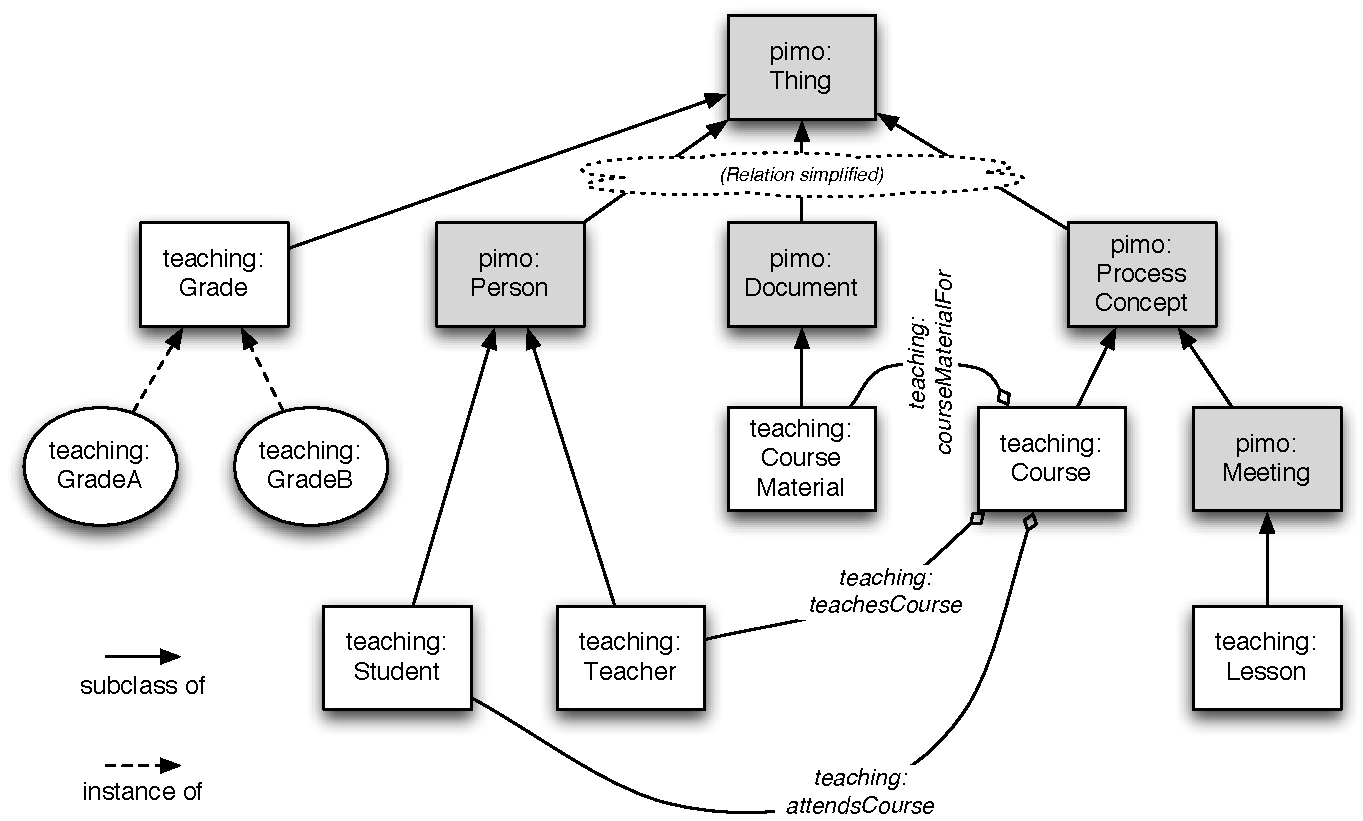
\includegraphics[width=\linewidth]{images/PIMOextensionExample-Teaching}
    \caption{Extending PIMO with new classes, properties and instances for the domain of teaching}
    \label{fig:extensionExampleTeaching}
  \end{center}
\end{figure}

\begin{figure}
  \begin{center}
	\begin{verbatim}
# new classes:
   teaching:Grade a rdfs:Class;
      rdfs:subClassOf pimo:Thing.

   teaching:Student a rdfs:Class;
      rdfs:subClassOf pimo:Person.

   teaching:Teacher a rdfs:Class;
      rdfs:subClassOf pimo:Person.

   teaching:CourseMaterial a rdfs:Class;
      rdfs:subClassOf pimo:Document.

   teaching:Course a rdfs:Class;
      rdfs:subClassOf pimo:ProcessConcept.

   teaching:Lesson a rdfs:Class;
      rdfs:subClassOf pimo:Meeting.

# new properties and their inverse:
   teaching:courseMaterialFor a rdf:Property;
      rdfs:subPropertyOf pimo:partOf;
      rdfs:domain teaching:CourseMaterial;
      rdfs:range teaching:Course;
      nrl:inverseProperty teaching:hasCourseMaterial.
   teaching:hasCourseMaterial;
      rdfs:subPropertyOf pimo:hasPart;
      rdfs:domain teaching:Course;
      rdfs:range teaching:CourseMaterial;
      nrl:inverseProperty teaching:courseMaterialFor.

   teaching:teachesCourse a rdf:Property;
      rdfs:subPropertyOf pimo:related;
      rdfs:domain teaching:Teacher;
      rdfs:range teaching:Course;
      nrl:inverseProperty teaching:taughtBy.
   teaching:taughtBy a rdf:Property;
      rdfs:subPropertyOf pimo:related;
      rdfs:domain teaching:Course;
      rdfs:range teaching:Teacher;
      nrl:inverseProperty teaching:teachesCourse.
      
   teaching:attendsCourse a rdf:Property;
      rdfs:subPropertyOf pimo:related;
      rdfs:domain teaching:Student;
      rdfs:range teaching:Course;
      nrl:inverseProperty teaching:attendeeStudent.
   teaching:attendeeStudent a rdf:Property;
      rdfs:subPropertyOf pimo:related;
      rdfs:domain teaching:Course;
      rdfs:range teaching:Student;
      nrl:inverseProperty teaching:attendsCourse.

# new instances:
    teaching:GradeA a teaching:Grade;
      nao:prefLabel "A".

    teaching:GradeB a teaching:Grade;
      nao:prefLabel "B".

    ...
	\end{verbatim}
    \caption{Extending PIMO with new classes, properties and instances for the domain of teaching --- N3 code}
	\label{fig:extensionExampleTeachingN3}
\end{center}
\end{figure}

\paragraph{Inheritance} % (fold)
\label{par:inheritance}

Sub-classing any class from PIMO (whether it be existing classes from PIMO-upper or classes that have been added later) also means that the new sub-class can be used with the same properties that have been defined with its superclass. Remember that NRL has a closed world assumption, and not an open world assumption, as RDFS traditionally has. In NRL\footnote{\url{http://www.semanticdesktop.org/ontologies/nrl/}}, ontologies can be used to validate statements.
%\note{reference to NRL spec --- 05.01.08, done}
E.g., if the property \texttt{name(pimo:Person, String)} has been defined, and if we define our new class \texttt{teaching:Student} to be a sub-class of \texttt{pimo:Person}, then this will allow us to use \texttt{name} with instances of \texttt{Student} as well - an NRL validator will permit this, because all instances of \texttt{Student} are also instances of \texttt{Person}. An example of this is shown in Fig.~\ref{fig:propertyInheritance}: this concept is very similar to the idea of inheritance in object-orientation, even though strictly speaking it is not the same.

% paragraph inheritance (end)

\begin{figure}
  \begin{center}
	\begin{verbatim}
		
   pimo:name a rdf:Property;
      rdfs:Domain pimo:Person;
      rdfs:Domain rdfs:Literal.
		
   teaching:Student a rdfs:Class;
      rdfs:subClassOf pimo:Person.

   knud a teaching:Student;
      pimo:name "Knud M�ller".

	\end{verbatim}
    \caption{``Inheritance'' of properties}
	\label{fig:propertyInheritance}
\end{center}
\end{figure}

% subsection subclassing_pimo_upper (end)

\subsection{Markup for the new ontology}
\label{sec:extendingontologymarkup}
The teaching ontology still needs to be defined as proper NRL ontology
to be usable with PIMO. The ontology \textbf{must} to be identified via its URI
and the author of the ontology can be added
as \texttt{nao:creator}.

\begin{verbatim}
teaching:TeachingOntology a nrl:Ontology;
 nao:creator teaching:TeachingOntologyCreator.

teaching:TeachingOntologyCreator a nao:Party;
 rdfs:label "Knud M�ller".

\end{verbatim}

\subsection{Information Elements} % (fold)
\label{sub:information_elements}

An important feature of the NEPOMUK ontology architecture is the fact that it is divided into two tiers: the PIMO tier and the Native Structures tier, as defined in the NEPOMUK Information Element Ontology (NIE)\footnote{\url{http://www.semanticdesktop.org/ontologies/nie/}} and its sub-ontologies, such as the NEPOMUK File Ontology (NFO)\footnote{\url{http://www.semanticdesktop.org/ontologies/nfo/}}.
%\note{reference to NIE spec --- 05.01.08, done}
While the former covers the internal mental model of a user or an organization (people, events, projects, etc.), the latter covers the physical representations of data (address book entries, calendar entries, files, etc.). Obviously, there are numerous connections between the tiers: people are represented by address book entries, events appear in the calendar, projects have files associated to them.

Whenever classes that are introduced to PIMO have a physical representation on the user's desktop, a connection to NIE must be modeled as well. Consider the example of the teaching ontology above: Such an ontology will contain classes for Things like exams and essays. Those classes belong to the PIMO tier. Their representation within the computer --- e.g., as text files --- belongs to the native structures tier. Or, in a more complex case, the new ontology could very well come with a specialized application, such as a Training Course Manager, where users can assign attendees to trainings, etc. In this case, people and courses (PIMO tier) would be represented by the application as application-specific data structures or information elements (native structures tier). In both cases a link from the new PIMO classes to the information elements represented with NIE is required to fully exploit the possibilities of the semantic desktop.

% subsection information_elements (end)

%\note{Knud, 05.01.08: I decided to drop the Author class in the BibTeX example. Authors should really just be pimo:Persons, not a subclass thereof.
%Leo, 8/1: OK, DONE}

As a second example, we can consider an ontology for scientific publications. This ontology (which would probably be based on Bib\TeX), would come with classes such as \texttt{Article} or \texttt{Book} and relations between them like \texttt{bookContainsArticle} or \texttt{hasAuthor}. For the integration into PIMO, \texttt{Article} would most likely become a sub-class of \texttt{pimo:Document}. 
Documents have	two types: one which anchors them in the PIMO tier, and one which anchors them in the native structures tier.
The \texttt{pimo:LogicalMediaType} (and its sub-classes, e.g., \texttt{pimo:Document}) captures how a document is interpreted by the user and belongs to the PIMO tier. Logical media types can be contracts, invoices, assignments, invitations, law texts, etc. 
The other type, which is the \texttt{nfo:Document} type, captures how the system interprets the document, and belongs to the native structures tier.
This is the physical document type as modeled by NIE.
Instances of a logical media type can have various representations in the native structures tier: 
for example, a text interpreted as an invoice by the user can either be an \texttt{nfo:PlainTextDocument} or an \texttt{nfo:PaginatedTextDocument}. 
Vice-versa, one physical type can be used to represent both an invitation or an invoice, which are different logical media types.
Keeping this this separation of content and representation in mind, one can model concrete documents having two types, one on each tier.

\begin{figure}
  \begin{center}
\begin{verbatim}
bibtex:Article a rdfs:Class;
 # PIMO tier: interpreted by the user as nie:Document
 rdfs:subClassOf pimo:Document; 
 # native structures tier: interpreted by the system as nfo:TextDocument
 rdfs:subClassOf nfo:TextDocument. 

bibtex:hasAuthor a rdf:Property;
 rdfs:subPropertyOf pimo:related;
 rdfs:subPropertyOf nfo:creator;
 rdfs:domain bibtex:Article;
 rdfs:range pimo:Person.
 
bibtex:hasLCCN a rdf:Property;
 rdfs:subPropertyOf nao:identifier; \# add an identifier
 rdfs:domain bibtex:Article.
\end{verbatim}
    \caption{A Bib\TeX-based PIMO extension for scientific publications}
	\label{fig:bibtexExample}
\end{center}
\end{figure}
%bibtex:Author a rdfs:Class; 
% # this adds properties like Name
% rdfs:subClassOf pimo:Person. 

\subsection{Extension by Sub-classing from External Classes} % (fold)
\label{sub:extension_by_subclassing_from_external_classes}

\textbf{Another possibility is extending existing PIMO-upper classes by sub-classing them from external classes.} \emph{This is discouraged}. For example, if the class \texttt{pimo:Person} was defined a sub-class of \texttt{nco:PersonContact} and \texttt{pimo:Organization} a sub-class of \texttt{nco:OrganizationContact}, all instances of these classes would automatically be inferred to be \texttt{pimo:Thing}s. However, those instances would probably not have some of the properties required by the \texttt{Thing} defined, which would render the imported data invalid. 
Similarly, when a mapped class X has cardinality restrictions on its properties (such as required properties), adding X as new superclass to an existing PIMO class can render the instances of the PIMO class invalid. 

% subsection extension_by_subclassing_from_external_classes (end)

\subsection{Summary} % (fold)
\label{sub:summary}

The very condensed summary to extending PIMO and mapping frome existing ontologies to PIMO is the following:

\begin{itemize}
  \item Make classes sub-classes of PIMO-upper classes.
  \item Make properties sub-properties of PIMO-upper properties.
	\item Relations: Links between Things have to be browseable, properties should have inverse relations defined (see \cite{rohmer2005})
	\item Extensibility: Users are free to add new relation types and new classes (see \cite{rohmer2005})
\end{itemize}

% subsection summary (end)

\section{Importing Domain Ontologies into a User's PIMO}
\label{sec:importingontologies}
%\note{Written by Leo, but Knud: feel free to mash it up}
Once modeled, the new domain ontology such as the teaching ontology in the previous examples can be made available publicly for others, for example by publishing it on the Web. A good reference for doing this is \emph{Best Practice Recipes for Publishing RDF Vocabularies}~\cite{SWBPVocabularyRecipes}.

% adressing
Semantically, an imported ontology is captured using a \texttt{nrl:imports} statement.
When a user imports a domain ontology, this statement \textbf{should} be added.

{\small
\begin{verbatim}
claudia:Pimo nrl:imports teaching:TeachingOntology.
\end{verbatim}
}

%Importing the ontology to a Sematic Desktop or other Personal Information Management system can then be done by downloading the ontology file and storing it into the RDF store where the PIMO of the user is kept.
% Stuff like downloading is outside the scope of PIMO and really has no place in the PIMO specification
Once the user of a Semantic Desktop system imports an external PIMO into their own desktop, all new classes (which are sub-classes of \texttt{pimo:Thing}) \textbf{should} become available to them as if they had created those classes themselves.
Instances, on the other hand, are not automatically available.
As said in the introduction, the scope of a PIMO for an individual user is to model data that is within their own attention and needed for knowledge work or private use.
However, when importing external ontologies or knowledge bases, not all instances may be of interest to the user. As with imported information elements, a separate Thing is created to represent the imported resource within the PIMO of the user and connected to the imported instance using \texttt{pimo:hasOtherRepresentation}\footnote{An alternative would be to treat all Things present in the RDF data available of the user as if they were created by the user, imported or not. This has the drawback that it allows to represent the same real-world entity twice, first in the imported domain ontology and second in the user's own PIMO.}.
Before creating a new Thing for an imported instance, the PIMO of the user has to be checked if the entity is already represented as a Thing, as indicated above in Section~\ref{sec:creatingthingalgorithm}.
Once represented as a Thing in the user's PIMO, it is possible to assign a personal identifier to it, annotate it, and use it. 

Implementations \textbf{must} automate the importing process. The user should be able to interact with imported Things as if they were created by themselves. 

\begin{comment}
LEO: THIS COMMENTED OUT NOW, ITS TOO SCIENTIFIC.
\section{Design Rationale}
\label{sec:designrationale}
In this section the design rationale behind \pimo and the sources which influenced us are described. 
% COPIED FROM SauermannElstDengel2007
%The motivation for creating the PIMO is to find a language to name the terms
%that are relevant to a knowledge worker and to have ways to express facts about
%these terms. Once this language is defined and formalized in the ontological
%description of the PIMO, it can be used to translate existing resources, and to
%express information about them. The PIMO is a user-centric view on existing
%documents, domain ontologies, and web data sources.
%
%While the organization asks for universally applicable and standardized
%persistent structures, processes, and work organizations to achieve and
%maintain universally accessible information archives, the individual knowledge
%worker requests individualized structures and flexibility in processes and work
%organization in order to reach optimal support for the individual activities.
%
The vision behind this work is that a \emph{Personal Information Model} reflects and captures a user's
personal knowledge, \eg about people and their roles, about organizations, processes,
things, and so forth, by \emph{providing the vocabulary} (concepts and their relationships)
required for expressing it as well as concrete instances. In other words, the domain of a
\pimo is meant to be ``all Things and native resources that are in the attention of the
user when doing knowledge work''.
\note{Knud, 07.01.08: Probably quickly explain what native structures are?}
Though ``native'' information models and structures are
widely used, there is still much potential
for a more effective and efficient exploitation of the underlying knowledge. We think that,
compared to the cognitive representations humans build, there are mainly two shortcomings
in native structures:
\begin{itemize}
  \item \emph{Richness of models}: Current state of cognitive psychology
  assumes that humans build very rich models, encoding not
  only detailed factual aspects, but also episodic and situational
  information. Native structures are mostly taxonomy- or
  keyword-oriented.
  \item \emph{Coherence of models}: Though nowadays (business)
  life is very fragmented humans tend to interpret situations as a
  coherent whole and have representations of concepts that are comprehensive
  across contexts. Native structures, on the other hand, often
  reflect the fragmentation of multiple contexts. They tend to be
  redundant (i.e., the same concepts at multiple places in
  multiple native structures). Frequently, inconsistencies are the
  consequence.
\end{itemize}

The \pimo shall mitigate the shortcomings of native structures by providing a
\emph{comprehensive model} on a \emph{sound formal basis}.

% next snip
%When building concrete \pimos, we now have the
%problem of two, potentially conflicting demands: On the one hand, we want to give the user
%the opportunity to span his information space largely in the way \emph{he} wants. The
%\pimo should model \emph{his} mental models. In consequence, we cannot prescribe much of
%this structure. On the other hand, ``empty'' systems often suffer from the cold
%start problem, being not accepted by user when not already equipped with some initial content.
%Using a multi-layer approach (see also \cite{Sauermann+2006d}), we try to find a balance through providing 
%the presentational basis as given, which users \emph{can} incorporate or extend:
%by a layered approach to \pimos : The representational basis
%as well as the basic dimensions of a \pimo are pre-given, but flexible enough for simple as
%well as more advanced modeling. Lower levels are meant as a proposition; when establishing
%an individual \pimo, users \emph{can} incorporate them into their model if they find them
%adequate and useful, but they don't have to. In the following, we briefly sketch the
%proposed \pimo layers:

% NOTE: THIS IS BAD, PIMO-MID IS a FORBIDDEN WORD and therefore replaced with XXXXXXX
%\subsection{PIMO-Basic, PIMO-Upper, PIMO-XXXXXXX and Domain Ontologies}
%Apart from the native structures, the mental models are represented using a multi-layer
%approach. These layers are:
%\begin{itemize}
%  \item PIMO-Basic: defines the basic language constructs. The class
%  pimo-basic:Thing represents a super-class of other classes.
%  \item PIMO-Upper: A domain-independent ontology defining abstract sub-classes of
%  Thing. Such abstract classes are PersonConcept, OrganizationalConcept,
%  LocationConcept, Document, etc.
%  \item PIMO-XXXXXXX: More concrete sub-classes of upper-classes. The
%  mid-level ontology serves to integrate various domain ontologies and provides
%  classes for Person, Project, Company, etc.
%  \item Domain ontologies: A set of domain ontologies where each describes a
%  concrete domain of interest of the user. The user's company and its
%  organizational structure may be such a domain, or a shared public ontology.
%  Classes are refinements of PIMO-XXXXXXX and PIMO-Upper, allowing an integration
%  of various domain ontologies via the upper layers.
%  \item PIMO-User: the extensions of above models created by an individual for
%  personal use. Classes, properties and Things are created by the user.
%\end{itemize}

% END OF SauermannElstDengel2007
\end{comment}


\section{Practical Directions on Using PIMO}
In this section, a few issues that will arise in actual PIMO usage are discussed. For each of these issues, we will suggest a recommended way of handling them. Even though those things are not strictly speaking part of the ontology, they are part of the standard defining how to use the PIMO ontology in applications.
Implementers \textbf{should} conform to these directions.

\subsection{Creating Things}
\label{sec:creatingthingalgorithm}
New PIMO Things can be created freely, but usually the creation of a Thing is rooted in the existence of an information element.
An algorithm to create new Things based on information elements \textbf{should} follow these steps:

\paragraph{Start} The software agent encounters a resource with URI $X$ and wants to verify if the user already has knowledge about \textbf{$X$}. 
\paragraph{Check GroundingOccurrence} Query the user-PIMO for:
\begin{verbatim}
SELECT ?thing WHERE {?thing pimo:groundingOccurrence ?X.}
\end{verbatim}
When a Thing is found, finished.
\paragraph{Check occurrences} Repeat the last step to search if $X$ is an occurrence of a Thing.
\paragraph{Check identifiers} Validate if the InformationElement has an identifier or a referencing occurrence that is also used on an existing Thing. The information element is called an \textbf{occurrence} of a Thing when it shares the same identifiers. The correct query is:
\begin{verbatim}
SELECT ?thing  
WHERE {
?thing ?p ?o. 
?X ?p ?o. 
?p rdfs:subPropertyOf nao:identifier.
} UNION {
?thing ?p ?o. 
?X ?p ?o. 
?p rdfs:subPropertyOf pimo:referencingOccurrence.
}
\end{verbatim}
When a Thing is found, finished.
\paragraph{Create a new Thing}
When the last step did not return an existing Thing, this can be an indicator that element $X$ is new to the user and should be modeled with a new Thing. 
Mint a new URI and add the identity values from the InformationElement. 

In the following SPARQL query example, we assume that Claudia's System has just encountered a new calendar event $X$ and represents it using the new minted URI $claudia:Event42$. 
{\small
\begin{verbatim}
CONSTRUCT { 
<claudia:Event42> rdf:type pimo:Thing.
<claudia:Event42> ?i ?io.
<claudia:Event42> nao:prefLabel ?title.
<claudia:Event42> rdf:type  ?type.
<claudia:Event42> rdf:type  ?pimotype.
<claudia:Event42> pimo:groundingOccurrence ?X.
<claudia:Event42> nao:created ``2007-06-30T18:11:00Z''.
<claudia:Event42> pimo:isDefinedBy claudia:PIMO.
} WHERE {
OPTIONAL (?X ?i ?io. ?i rdfs:subPropertyOf nao:identifier.).
OPTIONAL (?X nie:title ?title).
OPTIONAL (?X rdf:type  ?type).
OPTIONAL (?X rdf:type  ?type. ?pimotype rdfs:subClassOf ?type.
 ?pimotype rdfs:subClassOf pimo:Thing).
}
\end{verbatim}
}
The different parts of this query are:
\begin{itemize}
	\item all identifiers are copied (?i, ?io)
	\item the title is copied for readability and to use it for tagging (?title)
	\item the original type(s) are copied (?type)
	\item find possible PIMO:Thing classes that can be used for this type (?pimotype)
	\item the groundingOccurrence relation is added
	\item the created timestamp is set to the current date
	\item the isDefinedBy relation is set
\end{itemize}
Finding a suitable class to represent the resource
in the PIMO depends on a mapping of information element classes to PIMO classes
and can be realized in different ways, see Section~\ref{sec:classofthing}.

\subsection{Changing the Type of a Thing}
\note{Knud, 06.01.08: Can we change "Thing" into "Instance" (also below)? To me, "thing" sounds much too ambiguous.
\emph{Leo, 8/1:}I would stick to \texttt{Thing} as a word used before}
Changing the type of an instance can lead to invalid statements in the knowledge base. E.g., this can happen when the instance in question is involved in statements using a property with a specific domain and range, and the new type is not compatible to those.
As this would render the model invalid, this situation must be avoided in applications interacting with PIMO data.
A user interface should remind the user of possible problems and should suggest solutions. 

\note{Knud, 06.01.08: Is it even possible that domain and range are not set in NRL? If not, maybe remove this paragraph. 
\emph{Leo, 8/1:} NRL does not require it} A different approach is ontology-by-examples where the main principles is that ``the user is always right'' and domain/range values are not explicitly set but implied by previous usage. 
User interfaces may support this behavior by setting the domain and range to \texttt{pimo:Thing} and suggest properties suitable for class by analysing previous usage of the property.

\subsection{Deleting a Thing}
We can say that, in RDF, instances do not exist independently, but only as part of statements. Thus, ``deleting an instance'' really means deleting all statements in which this instance is involved (as subject or object).
%Note, that also \texttt{pimo:creationSupportedBy} links will be deleted by this, which may result that an algorithm soon creates the instance again (if the user somewhere configured to created instances automatically). See below in section Automatic Creation of Things from ResourceManifestations. 
%In this case, it may be better to use the \texttt{pimo:metaHidden} property to hide it.
\note{Knud, 06.01.08: this needs to be explained, otherwise it's incomprehensible.
\emph{Leo, 8/1:} actually, the groundingForDeletedThing is the needed Thing, I described it.}
If the instance has a grounding occurrence relation, a new \texttt{pimo:groundingForDeletedThing} relation should be created to record the deletion.
Data integration algorithms analysing resource to automatically create Things can then avoid re-creating the already deleted Thing.

\subsection{Deleting User-generated Classes and Properties}
Deleting a user-generated class is allowed but requires that instances are re-typed to the direct super-class of the deleted class. Also the domains and ranges of all properties defined with the class as domain or range need to be changed to the direct superclass. 
These changes are necessary to prevent the model from becoming invalid.
Classes defined in the pimo language cannot be deleted, only classes defined by the user can be deleted.

The direct super-class $S$ of the class $C$ is defined as the class where no other class $T$ exists where $C$ has superclass $T$ and $T$ has superclass $S$. If there are multiple $S$, all of them should be used as replacement when deleting a class.

%\note{Knud, 06.01.08: Saying that something is ``forbidden'' sounds really strange. Also, why not just say: \emph{If user-generated properties are deleted, this requires all statements in which those properties are involved to be deleted as well, in order to prevent the model to become invalid. Alternativaly, all occurrences of the property could be replaced by its super-property.}
%\emph{Leo, 8/1:OK}} 
If user-generated properties are deleted, this requires all statements in which those properties are involved to be deleted as well, in order to prevent the model to become invalid. 
Alternatively, all occurrences of the property could be replaced by its super-property.
%This would be analogous to how classes are handled.} Deleting a user-generated property that was used as predicate in statements is forbidden, as it is not clear what the semantics of the statements would be nor what property should be used as replacement in the statements. User-generated properties can be deleted when all statements using them are deleted a priori.



\subsection{Merging Duplicates}
\label{sec:mergeduplicates}
\emph{Duplicates} are two Things that represent the same real-world entity within a user's PIMO. As we apply the unique name assumption (two Things with different names are different), duplicates should be found and corrected. 
When duplicates are found, both (the ``duplicate'' and the ``original'') can be merged into one single instance.
In this process, RDF statements involving the duplicate are changed so that they now refer to the original.
In a local setup with one desktop and all data stored in a single database, this process is without information loss and causes no side-effects. As Semantic Web applications are in a distributed scenario, deleting a duplicate resource can cause dangling links in related databases and other side-effects. 
\note{Knud, 06.01.08: The idea of dangling links here is a bit misleading here. It implies that the Thing the link refers to is somehow \emph{gone}. However, the Thing was never really there --- there are always only statements about Things.} 
\note{Leo: no, its ok. Deleting/merging Things may cause these problems the suggested
hasDeprecatedRepresentation fixes it like a 301 ``moved permanently''} 

For this, the \texttt{pimo:hasDeprecatedRepresentation} property \textbf{should} be used to relate the original with the (now deleted) duplicate. Note that the range of this property is not defined, as all data about the duplicate resource (including the type) is deleted.

When merging two duplicate resource $A$ and $B$ into one resource $C$, a few practical guidelines can reduce side-effects:
\begin{itemize}
	\item The URI of $C$ is either $A$ or $B$, the older resource (as defined by \texttt{nao:creationDate}, see Section~\ref{sec:changedates}) is to be preferred as it has a higher chance of being used.
	\item The classes of $C$ are the union of the classes of $A$ and $B$.
	\item All statements about $A$ and $B$ are merged to $C$.
\end{itemize}

\subsection{Unification of multiple Information Elements into one Thing}
\label{sec:unification}
In comparison to merging duplicate Things, \emph{unification} is the process when multiple information elements representing the same real-world entity are mapped to one \texttt{pimo:Thing} instance.

In PIMO, multiple information elements representing one real-world entity are mapped to exactly one \texttt{pimo:Thing} instance using the \texttt{pimo:groundingOccurrence} and \texttt{pimo:occurrence} relations. 
Algorithms or user interfaces implementing unification must consider the identifying properties of a Thing (see Section~\ref{sec:identification}) when searching for possible Things to representing information elements.
%If algorithms don't find an existing Thing to represent and information element, they should create a new instance. See Section~\ref{sec:classofthing} about suitable PIMO classes to represent information elements.

Four default \textbf{NRL Views} and \textbf{NRL ViewSpecifications} are defined for different levels of inference. Each creates a named graph that contains the instance data and the inferred statements.

\begin{description}
	\item[\texttt{pimo:InferOccurrences}] a view that infers occurrences based on \texttt{nie:identifiers} and pimo:referencingOccurrence annotations.
	\item[\texttt{pimo:GroundingClosure}] a view that adds statements about the grounding Occurrences and \texttt{hasOtherRepresentation} to a Thing.
	\item[\texttt{pimo:OccurrenceClosure}] a view that adds statements about all occurrences to a Thing.
	\item[\texttt{pimo:FullPimoView}] a supergraph of all above.
\end{description}

By providing these graphs, we let the user and software agent decide if the full closure is needed at all times. When no closure is needed, the plain NRL data graphs can be used as-is.
To answer complex queries like ``Which e-mails were sent to me by attendees of meetings that I have today'', the full closure is a good choice.

The ability to superimpose data using inference limits the data needed in a PIMO to a necessary minimum: only the identification properties are mandatory, the occurrence and the hasOtherRepresentation properties superimpose existing data. 

\begin{verbatim}
claudia:DirkHagemann a pimo:Person;
 pimo:occurrence <imap://claudia@example.com/INBOX/1#from>;
 pimo:groundingOccurrence <file://home/claudia/dirk.vcf#dirk>.
\end{verbatim}


Using the guiding example, an integrated view of Claudia on Paul is the following, assuming full closure:
{\small
\begin{verbatim}
# The canonical Dirk
claudia:DirkHagemann a pimo:Person;
# the second type is also inferred
 a nco:PersonContact;
 pimo:isDefinedBy claudia:PIMO;
 nao:prefLabel 'Dirk Hagemann';
 nao:identifier "dirk@example.com";
 pimo:occurrence <imap://claudia@example.com/INBOX/1#from>;
 pimo:groundingOccurrence <file://home/claudia/dirk.vcf#dirk>;
 pimo:referencingOccurrence <http://www.example.com/people/DirkHagemann>;
 pimo:hasOtherRepresentation <http://id.example.com/person/1650>;
# the inferred facts
 nco:hasEmailAddress <mailto:dirk@example.com>;
 nco:nameFamily "Hagemann";
 nco:nameGiven "Dirk";
 nco:photo <http://www.example.com/people/dirk/photo.jpg>.
 
# E-mail, now pointing to the canonical Dirk
<imap://claudia@example.com/INBOX/1> a nmo:Mail;
 nmo:from claudia:DirkHagemann.
\end{verbatim}
}

%From the perspective of the user, facts stated about grounding occurrences are correct (they have been taken from existing data managed by the user); as are hasOtherRepresentation 
%(they are from formal ontologies imported and accepted by the user). If this is not the case, the incorrect statements must not be integrated, which is interesting but out of the scope of PIMO for now.
%As a result of the unification process, one Thing points to multiple information elements. This is also reflected in the previous examples, such as this:

\subsection{Tagging and Annotating Files}
\label{sec:taggingfiles}
Conceptually, once an Information Element (a file, an e-mail, a webpage, an address book entry, etc.) 
is in the attention of the user
and is read or annotated, it is also a Thing in the mental model of the user.
A core idea of the Semantic Desktop is to use other Things as dimensions to annotate files and retrieve them later, as described in~\cite{Dengel2006}.

Lets assume the file \texttt{/home/claudia/doc/tripplan.pdf} is to be tagged with the  tag ``Belfast Meeting Package''.

A representation of the file is already extracted by the semantic desktop data wrapper system
(or any other content management system):

\begin{verbatim}
<file://home/claudia/doc/tripplan.pdf> a nie:TextDocument;
 nie:language "en";
 nie:title "Belfast Bus Timetable".
\end{verbatim}

Additionally, the city of Belfast and the Belfast meeting package already exist in the model, as well as a \texttt{MeetingPackage} class (which was either created by Claudia, or came as part of a shared domain/group ontology):
\begin{verbatim}
claudia:BelfastMeetingPackage a claudia:MeetingPackage, pimo:Tag;
 pimo:tagLabel "Belfast Meeting Package";
 pimo:isDefinedBy claudia:PIMO.
\end{verbatim}

To add a simple tag, the file is now represented as a Thing (\textit{thingified}) and
the tagging relation set.

\begin{verbatim}
claudia:BelfastBusTimetable a pimo:Document;
  nao:prefLabel "Belfast Bus Timetable";
  pimo:isDefinedBy claudia:PIMO;
  pimo:groundingOccurrence <file://home/claudia/doc/tripplan.pdf>;
  nao:hasTag claudia:BelfastMeetingPackage.
\end{verbatim}

The interested reader may now ask, ``but why create a new Thing and
not just add the nao:hasTag relation directly to the file?''
The reason to \textit{thingify} the file is twofold:
first, it is possible to assign a new class to the file, for example
creating the class \texttt{claudia:BusTimetable}. 
Second, the same timetable may be available in different data objects,
if it is stored in an e-mail attachment, a web resource,
or a local file --- it is always the same document.
A tag added to one occurrence of the file is also valid for other occurrences. Also refer to Sections~\ref{sec:pimoVSnie},\ref{sub:information_elements}.

Given Claudia finds the same timetable on a website, the system
can link the two based on \texttt{nie:identifiers} (which should be globally unique 
identifiers for information elements, independent of the data object
they are stored in). This example shows this case (with copied identifiers):

\begin{verbatim}
# the file on the harddisk
<file://home/claudia/doc/tripplan.pdf> a nie:TextDocument;
 nie:language "en";
 nie:title "Belfast Bus Timetable";
 # this isbn is fictional
 nie:identifier "ISBN:12123-123123".
 
<http://www.buseireann.ie/timetables/belfast.pdf>
 a nie:TextDocument;
 nie:title "Belfast Bus Timetable";
 # this isbn is fictional
 nie:identifier "ISBN:12123-123123".
 
claudia:BelfastBusTimetable a pimo:Document;
  pimo:isDefinedBy claudia:PIMO;
  pimo:groundingOccurrence <file://home/claudia/doc/tripplan.pdf>;
  pimo:occurrence <http://www.buseireann.ie/timetables/belfast.pdf>;
  nie:identifier "ISBN:12123-123123";
  pimo:hasTag claudia:BelfastMeetingPackage.
\end{verbatim}
The tag assigned to the bus time table is now valid,
independent of the data object.

Using the generic tag relation \textbf{pimo:hasTag} is 
an easy-to-use entry point for users that don't need
formal semantic relations.

Using the property \emph{nao:hasTag} is not sufficient
to be PIMO conformant, implementers \textbf{must} use
the \emph{pimo:hasTag} relation for desktop tagging.
The \emph{nao:hasTag} property and \emph{nao:Tag} class are reserved for data of information elements that are imported into a PIMO.

\textbf{Example}: The Belfast Bus Timetable has the topic Belfast,
which is not just a Tag but says more about the relation between the 
timetable and the city. The \textbf{has Tag} relation can be used for this:
\begin{verbatim}
claudia:BelfastBusTimetable a pimo:Document;
 pimo:hasTag claudia:Belfast.
\end{verbatim}

\textbf{Example}: The relation between Claudia and the 
BelfastMeetingPackage can be expressed using ``has tag'' but 
may also be represented with a relation saying more about
the semantics: Claudia is ``attending this meeting''. 
Assuming that the MeetingPackage is a sub-class of meeting,
this could be expressed like:
\begin{verbatim}
claudia:BelfastMeetingPackage a meeting:MeetingPackage.

# instead of nao:hasTag, a semantic relation is used
claudia:Claudia pimo:attendee claudia:BelfastMeetingPackage.
\end{verbatim}

\subsection{Geo-locating Things}
Things can be geo-located, meaning that their geographical location is set using latitude, longitude and altitude information in the WGS84 geodetic reference datum.
In PIMO, the location is a separate entity of type \texttt{Location}, and other items can then be geo-located there. The relation \texttt{pimo:hasLocation} is used for this, \texttt{pimo:isLocationOf} is the inverse.
There is an abstract marker class for locatable Things: pimo:Locatable.
Social events, organizations, persons, and physical objects are locatable. 

To add a location to a meeting, this data is added, for your reference the location is also given:
\begin{verbatim}
claudia:InitialMeetinginBelfast a pimo:Meeting;
  nao:prefLabel "Initial Meeting in Belfast";
  pimo:hasLocation claudia:Belfast.
  
claudia:Belfast a pimo:City;
  nao:prefLabel "Belfast";
  geo:lat "54.5833333";
  geo:long "-5.9333333".
\end{verbatim}

Usually, locations should be reused to locate multiple Things,
but new locations can of course be generated anytime.

PIMO defines a number of general-purpose classes for countries, states, cities, buildings, and rooms, which we consider independent of culture and domain. Domain-specific ontologies can specify those classes further.
In the rare case when the type of location cannot be specified with any of the existing classes, the superclass \texttt{pimo:Location} can be used.
In some application scenarios (such as geo-locating a large amount of photos or measurement values), many locations would be needed.
To simplify annotation and remove clutter, specialized vocabularies may
then be used, as for example done in the NEXIF vocabulary for photos.

\subsection{Defining what is in the PIMO and what is not: NRL Graphs and \texttt{definedBy}}
\label{sec:nrlgraphs}
The facts (i.e., the statements) used to describe Things should be kept in named graphs according to the NRL standard. This allows to express metadata about the facts, such as to which
PIMO the Things belong (see Sect.~\ref{sub:connectingThingsToPimo}) or when individual triples were changed (see Sect.~\ref{sec:changedates}) and by whom.
Another important feature is to find which Things are in the user's PIMO and 
which not. In a shared environment, users may often import group-level ontologies that contain 
Things modeled by others. Considering this, it is important to keep up-to-date as to who said what, or, in other words, to detect if a Thing was modeled by the user or not.

All data expressed about Things can be kept in NRL graphs. 
The minimal metadata is:
\begin{itemize}
	\item The type of the graph is \texttt{nrl:KnowledgeBase}, as it can contain both instances and ontology constructs (see the NRL specification for more details).
	\item The graph is imported into the user's PIMO.
\end{itemize}
Additional metadata such as \texttt{nao:created} can be added.
These facts can be expressed in a separate metadata graph.
An example of how this looks like in code using Trig Notation\footnote{\url{http://sites.wiwiss.fu-berlin.de/suhl/bizer/TriG/}}:

\begin{verbatim}
# The instance data
claudia:graph1 {
  claudia:DirkHagemann a pimo:Person;
    nao:prefLabel 'Dirk Hagemann'.
}
# The metadata
claudia:graph1_metadata {
  claudia:graph1 a nrl:KnowledgeBase;
  claudia:PIMO nrl:imports claudia:graph1.
}
\end{verbatim}


\textbf{As not all implementers can or want to use NRL graphs to keep track of the boundaries of a PIMO, 
\texttt{pimo:isDefinedBy} must be used} to connect classes, properties, and instances to the PIMO that defines them\footnote{Separation based on the namespace was considered by some to be enough, but is not (as stores use fulltext comparison to handle namespaces, namespaces as such don't exist in RDF but only in XML).}.

To support both ways of detecting the boundaries of a user-PIMO, 
implementations \textbf{may} add the NRL metadata in addition to the \texttt{pimo:isDefinedBy} 
statements to the generated data. 
Resulting in:

\begin{verbatim}
# The instance data
claudia:graph1 {
  claudia:DirkHagemann a pimo:Person;
    pimo:isDefinedBy claudia:PIMO.
    nao:prefLabel 'Dirk Hagemann'.
}
# The metadata
claudia:graph1_metadata {
  claudia:graph1 a nrl:KnowledgeBase;
  claudia:PIMO nrl:imports claudia:graph1.
}\end{verbatim}

%This may produce legal but not valid NRL data, as explained in the NRL specification, Section 2.3.4
%\footnote{\url{http://www.semanticdesktop.org/ontologies/nrl/\#mozTocId220340}}.
%\note{Knud, 06.01.08: What does \emph{legal but not valid} mean?
%\emph{Leo, 8/1:}added link to NRL. DONE}

%\subsection{Annotating Websites}
% LEO: I cut that section, when we already have files, we don't need websites anymore.

%\subsection{Annotating an Event with NIE and PIMO}
% LEO: I cut that section, when we already have files, we don't need Event anymore.

\begin{comment}
\subsection{Annotating Resources without Creating New Things}
\label{sec:annotatingexternalresources}
\note{Knud, 06.01.08: To be honest, I find this section a bit esoteric (and I also admit I probably don't fully understand it). Do we really need this in the PIMO-Spec? I feel like we should try to keep the spec concise and drop this (would be nice in a paper, but not here).}
The interested reader may have come to the conclusion, that the suggested
way of handling annotation in PIMO is complicated and cumbersome; based 
on the observation that to annotate a file, a new ``Thing'' resource
has to be created. Creating a Thing requires minting a new URI, describing
it and linking it to the annotated resource using the \texttt{pimo:groundingOccurrence}
relation.

There are two reasons for this approach:
\begin{itemize}
	\item From a philosophical point of view, the resource can exist without the user's observation of it.
	The user annotates what perception and interpretation they have of the resource,
	a personal perspective. To represent it, the resource is ``thingified'', a new URI is minted,
	to represent that the ``user views the resource''.
	\item Technically, a newly minted URI inside the user's namespace has some qualities that
	make it a good RDF URI: it is retrievable, it does not change, it is unique.
\end{itemize}

But this also implies, that once a system satisfies both reasons, no new URI has to be minted.
A Semantic Web system to handle resources could fulfil these requirements:
\begin{itemize}
	\item Allow users to express their personal view on resources in a way that 
	represents ``this user has that view on resource X''. A possible technical 
	realization of this requirement is to use graph-metadata to annotate
	which triples are created by which user. The NRL specification allows this.
	\item URIs of resources have to be \textbf{retrievable}. Today, only a few web-applications
	hosting URIs fulfil all requirements of the Technical Architecture Group (TAG) 
	of the W3C towards Semantic Web URIs\footnote{See the decision taken to answer the
	http-range-14 issue at \url{http://lists.w3.org/Archives/Public/www-tag/2005Jun/0039.html}}.
	A human-friendly version of these requirements
	is written in \cite{Sauermann+2007a}. Simplified, servers must implement HTTP GET content 
	negotiation and return either RDF or HTML representations.
	\item An URI must not change. Some content management systems don't fulfill this,
	also none of the common file systems (when a file is moved, the URI changes)
	nor does it the IMAP URI scheme.
\end{itemize}

Simply put: the system storing resources to be annotated must be fully Semantic Web and NRL compliant.
Such resources could then be annotated directly, without creating Things and relating them to grounding occurrences.

\textbf{Example}: annotating a correct Semantic Web URI without creating a new URI for it.
\begin{verbatim}
# It is mandatory that the used URIs conform to the open linked data standards
@prefix claudia: <http://www.example.com/people/claudia#> .

# The annotation is about Tim Berners Lee,
# identified by a correct Semantic Web URI 
@prefix timblcard: <http://www.w3.org/People/Berners-Lee/card#>.


# A named graph containing the metadata about Graph1
claudia:Graph1Meta {
 claudia:Graph1 a nrl:KnowledgeBase;
   nao:creator claudia:Claudia.
 # The annotations are now part of her user-PIMO
 claudia:PIMO nrl:imports claudia:Graph1.
}
# This is the annotation by Claudia about Tim Berners Lee
claudia:Graph1 {
  # Claudia says: he is a Person
  timblcard:i a pimo:Person;
   # he is now also part of Claudia's personal view on the world,
   # this is valid within this graph
   pimo:isDefinedBy claudia:PIMO;
   # a tag is added
   nao:hasTag claudia:SemanticWeb.
}
\end{verbatim}
We would recommend to try this out experimentally, when you have access to 
a system that fulfils the requirements,
but not before. 
Without a proper NRL implementation, misleading information
could be inferred.
The PIMO framework is intended to work today,
therefore the pimo:groundingOccurrence relation and the minting of new
URIs is recommended. It is also compatible for
the next years, when Semantic Web and NRL compliant systems exist.
\end{comment}

\subsection{Using NAO and NIE Elements for Annotation}
\label{sec:usingnieinpimo}
Throughout this document, we have shown several uses of NAO and NIE elements
that can be applied to \texttt{pimo:Thing} instances. 

Semantically, we start from the assumption that a Thing modeled in PIMO is describing a concept from the real world.
On the other hand, the Thing itself can be viewed as a set of statements or triples stored in a computer system.
Thus, Things are resources and can be annotated with NAO.
Also, using PIMO closure as described in Sect.~{\ref{sec:integratingfacts},
facts of NIE elements can be inferred as facts of PIMO Things.
Thus, Things can also have a NIE class as type.

In Table~\ref{tab:SemanitcsOfNIEInPIMO} we give an overview of how the semantics of
the predicates may alter when interpreted within the PIMO.

The text ``\textbf{no change}'' means that the interpretation is unchanged, ``\textbf{not interpreted}'' means you should avoid interpreting this property in PIMO. You may notice that some properties are not interpreted because they have DataObjects or Strings as range, where PIMO has properties modeling the same semantics but using other \texttt{pimo:Thing}s as range, which is a more precise way of modeling because of the UNA.
``\textbf{Required}'' means that this property is required for all instances of \texttt{pimo:Thing}
and this can be validated using the rules from Section \ref{sec:validationrules}.
``\textbf{Recommended}'' means that you should use this property as if it is required, but it cannot be validated in NRL as property restrictions are only available in OWL.

The properties describing how information is stored (mime-type, bytesize, characterset) are obsolete for Things, as they describe a serialization.

\begin{table}[h!tbp]
	\centering
		\begin{tabular}{|l|p{0.7\textwidth}|}
		  \hline
			Term & Semantics\\
			\hline
			\texttt{nao:created} & \textbf{Recommended} When the RDF Resource representing this Thing was first created in the user's PIMO.\\
			\texttt{nao:identifier} & no change, used for identification and matching.\\
			\texttt{nao:lastModified} & \textbf{Recommended} When the Resource representing this Thing was last changed in the user's PIMO. Note that it can be different from the nie:contentLastModified property of a groundingOccurrence. When blending multiple groundingOccurrences into a Thing, the latest contentLastModified should be chosen.\\
			\texttt{nao:modified} & \textbf{Recommended}\\
			\texttt{nao:personalIdentifier} & \textbf{Not recommended}, \texttt{pimo:tagLabel} \textbf{must} be used.\\		
			\texttt{nao:prefLabel} & \textbf{Recommended}\\			
			\texttt{nie:characterSet} & \textbf{Not interpreted}, obsolete in RDF\\
			\texttt{nie:comment} & no change\\
			\texttt{nie:contentCreated} & \textbf{Not interpreted} \\
			\texttt{nie:contentLastModified} & \textbf{Not interpreted} \\
			\texttt{nie:contentSize} & \textbf{Not interpreted}, obsolete in RDF\\
			\texttt{nie:copyright} & no change, can be set by the user when sharing Things with others. See also nie:legal\\
			\texttt{nie:depends} & no change\\
			\texttt{nie:description} & no change\\
			\texttt{nie:disclaimer} & \textbf{not interpreted}\\
			\texttt{nie:generator} & no change, \texttt{pimo:Things} can be generated automatically by software or manipulated by user interfaces\\
			\texttt{nie:generatorOption} & no change\\
			\texttt{nie:hasPart} & \textbf{not interpreted}, \texttt{pimo:hasPart} should be used\\
			\texttt{nie:identifier} & no change\\
			\texttt{nie:isStoredIn} & \textbf{not interpreted}, \texttt{pimo:isDefinedBy} covers the storage.\\
			\texttt{nie:keyword} & \textbf{not interpreted}, should be modeled using hasTag and assigning the keyword as title of the topic.\\
			\texttt{nie:language} & no change\\
			\texttt{nie:legal} & no change, by default all legal properties scope all the statements having the same subject as the legal statement\\
			\texttt{nie:license} & no change\\
			\texttt{nie:licenseType} & no change\\
			\texttt{nie:links} & \textbf{not interpreted}, use pimo:related or pimo:hasTag\\
			\texttt{nie:mimeType} & \textbf{not interpreted}, obsolete in RDF\\
			\texttt{nie:plainTextContent} & no change\\
			\texttt{nie:relatedTo} & \textbf{not interpreted}, use pimo:related\\
			\texttt{nie:subject} & \textbf{not interpreted}, use pimo:hasTag\\
			\texttt{nie:title} & \textbf{not interpreted}\\
			\texttt{nie:version} & no change\\
			\hline
		\end{tabular}
	\caption{Semantics of NAO and NIE in PIMO}
	\label{tab:SemanitcsOfNIEInPIMO}
\end{table}

\begin{comment}
\subsection{Isn't Reification Enough for a Personal View?}
\note{Knud, 06.01.08: For this section (though good), I have the same comment as before: I consider it to be outside the scope of a concise specification. Someone who is new to the whole SemDesk Thing and wants to work with it, will want to read this spec asking "ok, now how do I use PIMO". They will not want to know why certain decisions where \emph{not} taken. They will want to look up how stuff works, not how it \emph{doesn't} work. This section would be more appropriate in a document about the design decisions behind PIMO. Just my opinion!}
\note{Leo: moved to http://dev.nepomuk.semanticdesktop.org/wiki/OntologiesHowTo}
The Semantic Web provides another possibility to express a personal view on information elements, namely using normal annotations to the existing elements (by adding triples to them) and then reifying the triples and annotating them as ``being expressed as personal view''. Using named graphs and NRL is conceptually the same to reification and could also be used for this.
The reasons not to use reification or Named Graphs as primary modeling concept are both technical and political:
\begin{itemize}
  \item Data expressed in PIMO should be long-lasting and not be influenced by changes of operating systems, applications or the movement of files. To ensure this, the primary URIs of Things are generated in a separated namespace, tied to the user. 
  \item When Information Elements move, are deleted or are not accessible by the user anymore, they can be found again based on the identifying properties annotated to the stable URIs minted for Things.
  \item Using annotations on existing URIs would make the decision for the ``primary'' URI for a Thing ambiguous. The structure of Things implies that there is one primary representation, the Thing with its minted URI, pointing to all other representations using relations. 
  This allows implementations to quickly find the focus point (the Thing) from which all other information about it can be found. Although this is typically handled by inference engines, the current approach allows to find various sources of information about a Thing in the globally distributed Semantic Web, where distributed inference is not available.
	\item Reification is often criticized as being complicated, basing the whole system on it would direct this critique in the wrong direction.
	\item From a philosophical point of view, each individual sees and perceives the world through their own eyes and interprets it according to their own mental model. 
\end{itemize}
\end{comment}

\begin{comment}
\subsection{Why not Use owl:sameAs?}
\label{seq:faqsameas}
\note{Knud, 06.01.08: as before. Is this necessary in a specification document?}
\note{LEO: moved to http://dev.nepomuk.semanticdesktop.org/wiki/OntologiesHowTo}

OWL's \texttt{sameAs} is an equivalence relation (transitive, reflexive, symmetric) whereas \texttt{groundingOccurrence} is directed and inverse functional. 
To express that a Thing and an entity from a domain ontology are modeling the same concept from the real world, and that users have agreed on that, use \texttt{pimo:hasOtherRepresentation} (or \texttt{pimo:hasOtherConceptualization} for classes).

Connecting two resources with owl:sameAs implies that they refer to the same real-world entity. As PIMO is subjective, \texttt{pimo:groundingOccurrence} expresses that from the point of view of the user, they are the same, but not necessarily for other users. Using \texttt{sameAs} would create \texttt{n!} relations between \texttt{n} same objects, a fully connected graph. Given an \texttt{InformationElement} as input, querying what Thing has this as a grounding occurrence returns in one step the correct single answer, using a simplest query possible. This cannot be done using \texttt{owl:sameAs}, because the answers are possibly many InformationElements from the model, the unique Thing being one of them, only distinguished by its class being a sub-class of \texttt{pimo:Thing}. So the separation has the semantic reason that the view is directed from the user towards his InformationElements, and the technical reason that this allows an efficient realization in possible implementations.
\end{comment}
\begin{comment}
\subsection{Why isn't skos:Concept Used?}
\note{Knud, 06.01.08: specification?}
\note{LEO: moved to http://dev.nepomuk.semanticdesktop.org/wiki/OntologiesHowTo}
The interested reader may suggest to use \texttt{skos:Concept} instead of \texttt{pimo:Thing.} But then, all resources would have the same type, namely \texttt{skos:Concept}. Then all domain/range, sub-class and sub-property features of RDF are not usable and existing ontologies (such as NRL or NIE) 
cannot be used to model Things. This is visible when looking at the \texttt{skos:narrowerInstantive} property, which is a parallel approach to \texttt{rdf:type}.
We have tried SKOS in an evaluation and implemented a prototype using it during the EPOS project, coming to this conclusion.
\end{comment}

\subsection{How to Infer Knowledge Using Rules?}
The presented ontology may be used to express facts that can 
be used to infer new knowledge. For example, the person Claudia may be working
on the project ``CID''. Claudia is also employed by the company Example Inc. --- 
this may be used to infer that the company Example is involved in ``CID''
Such rules are very useful to improve the results when querying, as they will provide more answers.

In PIMO and NRL, it is not straightforward how to express these rules.
Also, as PIMO-upper is generic, any rules defined on this level may
not apply in all group-level ontologies.

We recommend to express such rules using a rule language (such as the
ones defined by the RIF working group of W3C\footnote{\url{http://www.w3.org/2005/rules/}}) or SPARQL-create statements.
These should be part of domain and group ontologies.

\section{Rules Defined by PIMO}
\label{sec:pimorules}
Some of the  rules defined in PIMO cannot be expressed using ordinary NRL semantics. These rules are written here using SPARQL construct queries \textbf{and are also part of the ontology, by virtue of \texttt{nrl:RuleViewSpecification}}.
The rules help to infer additional statements or validate a model.
\textbf{All rules in this section assume that at least the sub-class and sub-property 
relations are inferred.} 

\subsection{Construction Rules}
\label{sec:creationrules}
The first set of rules define new information that is inferred from existing data. They are used for integrating facts about Things by blending, see Sect.~\ref{sec:integratingfacts}.
The rules are expressed based on the assumption that Tbox inferenced facts are available in querying, whereas Abox inference may or may not. This means, sub-class and sub-property relations are fully inferred, but the statements implied by them may or may not\footnote{In instance bases, rules rdfs7 and rdfs9 make the majority of inferred statements and for storage optimization \url{http://www.w3.org/TR/rdf-mt/\#RDFSRules}}.
For some of the rules, the semantics of equality comparison is clearer under this assumption.
For example, assume two sub-properties of \texttt{nao:identifier}: \texttt{book:number} and \texttt{person:number}, both with a range of integer and values starting with numbers from 0.
Expressing a rule as ``two Things are equal when their \texttt{nao:identifier} is equal'' 
could imply, that a book is equal a person.

\textbf{\texttt{pimo:InferOccurrences} Level}: These are the rules to infer what resources are occurrences of Things based on identifiers. You can use this approach to integrate data from large stores. For example to see all appearances of a document using the document's NIE-identifier, this query searches for the \texttt{pimo:occurrence} relations.
\begin{verbatim}
CONSTRUCT {
?thing pimo:occurrence ?occurrence.
} WHERE {
?i rdfs:subPropertyOf nao:identifier.
?thing ?i ?value.
?occurrence ?i ?value.
}
\end{verbatim}

\textbf{\texttt{pimo:GroundingClosure} Level}: This adds all facts from grounding occurrences and \texttt{hasOtherRepresentation} occurrences to Things.
\begin{verbatim}
CONSTRUCT {
?thing ?p ?o
} WHERE {
?thing pimo:groundingOccurrence ?x.
?x ?p ?o.
}
CONSTRUCT {
?s ?p ?thing
} WHERE {
?thing pimo:groundingOccurrence ?x.
?s ?p ?x.
}
CONSTRUCT {
?thing ?p ?o
} WHERE {
?thing pimo:hasOtherRepresentation ?x.
?x ?p ?o.
}
CONSTRUCT {
?s ?p ?thing
} WHERE {
?thing pimo:hasOtherRepresentation ?x.
?s ?p ?x.
}
\end{verbatim}


\textbf{\texttt{pimo:OccurrenceClosure} Level}: This adds all facts of all occurrences to Things.
\begin{verbatim}
CONSTRUCT {
?thing ?p ?o
} WHERE {
?thing pimo:occurrence ?x.
?x ?p ?o.
}
CONSTRUCT {
?s ?p ?thing
} WHERE {
?thing pimo:occurrence ?x.
?s ?p ?x.
}
\end{verbatim}


\textbf{A broader Topic is also the Topic of a Thing.} If a Thing X has the tag A and topic A has a super topic B, then X has also the tag B. \texttt{superTopic} and \texttt{subTopic} are transitive.
\begin{verbatim}
CONSTRUCT {?x pimo:hasTag ?B} 
WHERE 
{?x pimo:hasTag ?A. 
?A pimo:superTopic ?B.}
\end{verbatim}
Note that this is not true for the \texttt{hasPart} relation.

An alternative to the \texttt{hasTag} rules would have been to represent topics as RDFS classes (instead of having them as instance of type \texttt{pimo:Topic}) and using \texttt{rdfs:subClassOf} relations instead of broader/narrower. But this has a nasty side-effect that for a topic like ``Web''  having a sub-topic ``Semantic Web'', the user would suddenly be able to create instances of ``Semantic Web'', this would be confusing.

\subsection{Validation Rules}
\label{sec:validationrules}
These rules validate a model. Some assumptions stated in the text can be validated using these rules. As a model for validation, we have chosen to pick a similar approach as the Jena validation engine, namely creating errors. The classes \texttt{error:Error} and \texttt{error:Message} were introduced for this purpose and not defined any further, we assume Errors can have parameters that are passed back as \texttt{error:param1}, \texttt{error:param2}, etc. The parameters can be referenced in the error message for readability.

\subsection{Rules Valid when Integrating with NIE}
When using PIMO in coordination with NIE, certain properties from NIE can be reused.
The rules are often used to restrict properties defined in the NIE ontology to be mandatory on \texttt{pimo:Things}, whereas they are optional when used on \texttt{nie:InformationElement}. Such restrictions are possible in OWL but not in NRL. 

\textbf{Every Thing must have a \texttt{nao:prefLabel}.}
\begin{verbatim}
CONSTRUCT {
_:err a error:Error.
_:err error:Message ``Thing \%1 does not have a nao:prefLabel''.
_:err error:param1 ?x.
} WHERE {
?x rdf:type pimo:Thing.
OPTIONAL { ?x nao:prefLabel ?title } .
FILTER (!bound(?title))
}
\end{verbatim}

\textbf{Every Thing must have \texttt{nao:created}.}
\begin{verbatim}
CONSTRUCT {
_:err a error:Error.
_:err error:Message ``Thing \%1 does not have a nao:created''.
_:err error:param1 ?x.
} WHERE {
?x rdf:type pimo:Thing.
OPTIONAL { ?x nao:created ?created } .
FILTER (!bound(?created))
}
\end{verbatim}

\section{Sources considered for designing PIMO}
Several ontologies and scientific publications predate this specification.
A definition of the term PIMO was given in~\cite{sauermann+2007b}:
\begin{definition}
A PIMO is a Personal Information Model of one person. It is a formal representation of
parts of the users Mental Model. Each concept in the Mental Model can be represented using
a Thing or a sub-class of this class in RDF. Native Resources found in the Personal
Knowledge Workspace can be categorized, then they are occurrences of a Thing.
\end{definition}

%COPIED FROM SauermannElstDengel2007
A similar approach was used by Huiyong Xiao and
Isabel F. Cruz in their paper on ``A Multi-Ontology Approach for Personal
Information Management'', where they differentiate between \emph{Application
Layer, Domain Layer and Resource Layer}. Alexakos et al. described ``A
Multilayer Ontology Scheme for Integrated Searching in Distributed Hypermedia''
in~\cite{likothanasis+2005}. There, the layers consist of an\emph{ upper search
ontology layer, domain description ontologies layer, and a semantic metadata
layer}.

PIMO is different from Topic Maps (TM) in that it is based on the logical and semantic foundations of RDF and RDFS, whereas TM have no such foundation.
A major difference between TM and RDF is that Topic Maps Associations are n-ary relations,
whereas in RDF relations are always binary.
In RDF, a similar approach as to TM is the SKOS vocabulary~\cite{SkosStandard}.
It represents all Things using the class \emph{Concept}, this prohibits reusing inference and typed properties of concepts (e.g., the ``first name'' property of a person cannot be modeled in SKOS).
%END OF SauermannElstDengel2007

% THIS was good for Leos diss and leo has not to forget to copy/paste it there
The idea of mapping SKOS, RDF, OWL and topic maps with upper ontologies has come up repeatedly, but with varying outcome. We value these articles as very important for our work, because of their excellent research and the experience of the authors.
\begin{itemize}
  \item Pepper and Schwab~\cite{Pepper+2003} try to map the identification approach of XML Topic Maps to RDF, leaving a few issues open. 
  \item Jack Park and Adam Cheyer mapped Topic Maps to Semantic Desktops for Personal Information Management in \cite{Park+2005}. 
  \item The \emph{Semex} system provides ideas about reference reconciliation~\cite{DongH2005}
  \item Jerome Euzenat proposed a top-level ontology for PIM in light of FOAF\footnote{\url{http://www.w3.org/2001/sw/Europe/200210/calendar/SyncLink.html}}
  Although this is a small, seemingly unimportant footnote, it shows how often capable people tried to address this problem.
  \item User Profile Ontology version 1\cite{UserProfileOntologyVersion1},
  mentioned in \cite{DELOSTIM2007}\footnote{\url{http://oceanis.mm.di.uoa.gr/pened/?category=publications}}.
%  \item Richard Saul Wurman found: geographical, alphabetically,
%  by Time, by Categories, by Hierarchy.
%  (Location, Alphabet, Time, Category, and Hierarchy, known as LATCH cite R. Wurman, D. Sume, and L. Leifer, Information Anxiety 2, Que, 2000.)
  \item Latif and Tjoa \cite{Latif+2006} map a user ontology against other top-level ontologies such as SUMO and DOLCE and use the LATCH approach from Richard Saul Wurman.
  %\item Nejdl's Beagle stuff. % too late to document this, we must finish now
\end{itemize}

% is this really true? Well, we comment it out
%They key factors that we found in most related work are \textbf{identifying resources unambiguously} and \textbf{modeling the complicated specializations in specialized domain ontologies} while keeping the core clean. So \textbf{integration of heterogenous data wins over trying to make a world-embracing super ontology}. 
%% do we agree on that?
%The PIMO approach, using the pimo:groundingOccurrence and the pimo:hasOtherRepresentation relations together with blending data, instead of using owl:sameAs seems (from our perspectice) the right choice.



\appendix
% THESE were part of development of this document
%\section{Open Issues}

\subsection{Ranking / Rating}
wait for tf-ont feedback


%\section{Issues Intentionally not handled by PIMO}

\subsection{Complex identifiers}
For identifiers that consist of multiple keys, or that go along more than one resource,
we need some way to capture them.

suggestion:
{\small
\begin{verbatim}

pimo:ComplexIdentifier a rdfs:Class.

pimo:ComplexIdentifierQueryBased a rdfs:Class;
  rdfs:subClassOf pimo:ComplexIdentifier.
  
pimo:complexIdentifierTriggerProperty a rdf:Property;
  rdfs:comment """The object property indicates that 
      the subject Query based complex identifier should 
      be triggered, when a resource has the property set. 
      For the email example, this would be 
      nco:hasEmailAddress""" ;
  rdfs:domain pimo:ComplexIdentifierQueryBased;
  rdfs:range rdf:Property .
  
pimo:complexIdentifierQuery a rdf:Property;
  rdfs:comment """Defines a query with one parameter, 
    ?x, that is to be filled in. The query selects 
    other variables (?y, ?z, ?a, ?number, etc.) that 
    have to be the same so that two entities can be 
    considered same. Example for e-mail: 
    SELECT ?x ?mail 
    WHERE {?x nco:hasEmailAddress ?e. 
           ?e nco:emailAddress ?mail.}"""
  rdfs:domain pimo:ComplexIdentifierQueryBased;
  rdfs:range rdf:Literal.
\end{verbatim}
}

\paragraph{Proposed Solution:} Mention that it is a problem, but give no indications for solution. Say that nao:identifier has to be enough.
Knud, Leo, Gunnar agree on this on 8.1.2008

\subsection{Modelling Default Properties and Things that have instances}
How to model the Book ``Moby Dick'' in the version published in
1960 with 300 pages? (example invented) 
It would be an instance of the class ``Book Edition''.

Now given I have a copy of the Book, then I have an instance of ``Book Copy'',
called ``Dirks's Moby Dick with Serial Number 123''.
Dirk's Moby Dick has also 300 pages, but may have a sticker on the cover
and an annotation of ``borrowed to claudia''.

The same problem arises with electronic gadgets, etc, every product.

\paragraph{Proposed Solution:} Leo: No Solutions, don't mention it.
Leo, Knud agree on this on 8.1.2008


\subsection{Associations implying Statements}
Current status (Knud and Leo via Skype, 12.9.2007):
We would say that this is useful and that statements and associations can be linked.

Revised by Leo on 13.12.2007: no time to work on this, finish the existing Things first.

A first suggestions for modelling it is in this document. 
Implementation is left open for now.

One major Thing is open:
subclassing from NAO,
I can only do that once the RDFS is fixed.

Another old idea I have to mention now, because it fits to the discussion:
The problem is that often, relations are not just a statement (=triple) but have some metadata,
or that N-Ary relations cannot be expressed using plain RDF. (In XML topic maps, they can)

Typical problem:
STATEMENT:
http://sap.com - foaf:member - http://sap.com/claudia.

A way to model this (this already in the PIMO last year)

ROLE:
x - type - pimo:Role;
 roleHolder - http://sap.com/claudia;
 roleContext - http://sap.com;
 roleValid - y.

y - type - pimo:Duration;
 beginTime "..."
 endTime "...".

Now, this is all pretty straightforward

To realize an effective way of doing all this, I propose to use a meta-modelling approach, where Associations (Role is a subclass of Association) are linked to imply statements of  certain property, and vice versa, that statements using a property imply that an Association must exist.

Using above model Role, this means:
STATEMENT -> ROLE.
ROLE -> STATEMENT.

> Looks good to me. But how would you link specific roles with specific properties, e.g. 'Member' with 'memberOf'? This is required for this to work.

like this:

pimo:Member pimo:impliesStatementRule
 "CONSTRUCT {?x pimo:hasMember ?y} WHERE {?association pimo:memberPerson ?y; pimo:memberOrganization ?x}".

This requires you to model the properties and classes beforehand:
* pimo:hasMember as the direct relation between person and organization,
* the Member class with properties
* pimo:memberPerson and
* pimo:memberOrganization.

is not done yet, but is probably interesting to do. 

%
\section{Issues solved by Agreement}
\subsection{Relation between PIMO:Thing and NIE:InformationElement}
\paragraph{Background} PIMO:Things are unique representations of concepts, such as a person, a book,
  a product, a company. For these, often ontologies exist already in NIE, 
  for example nco:PersonContact models people and a bibtex ontology for NIE may be soon available.
  To identify and distinguish pimo:Thing, an instance needs to have all identifying properties of occurrences attached, so for example a pimo:Event should get the NCAL ncal:uid as a property to match it and a pimo:Person should have the nco:contactUID as property. This helps finding them in the various databases available. 
  So ncal:uid and nco:contactUID should be possible properties for a pimo:Thing (or subclasses). Using a property from NIE with domain nie:InformationElement on a pimo:Thing infers that the Thing is a NIE:InformationElement. Also, the user may want to use the ontologies defined in NIE to annotate people and events, for example NIE defines a relation that a person can attend a meeting, this does not necessarily be remodeled again in PIMO.
  \paragraph{Problem} The properties defined in NIE should not be modeled again in PIMO. Sometimes properties from NIE should be usable on PIMO:Things.
  \paragraph{Solution pimo:Thing rdfs:isSubClassOf nie:InformationElement}
  This solution would allow us to reuse properties from NIE within PIMO without any problems. Also, as NIE properties are all optional, Things are not invalid because they miss some properties. For specialized classes, it is possible to make them subclasses of the specialized NIE classes (pimo:Person rdfs:subClassOf nco:PersonContact). 
  Advantage: we reuse NIE completly for modelling in PIMO.
  Disadvantage: this would bind the PIMO classes with NIE.
  \paragraph{Solution nie:InformationElement rdfs:isSubClassOf pimo:Thing}
  This was a rather bad idea, that came up when we didn't want the first solution.
  The trouble here is, that suddenly all InformationElements would be Things,
  even if they are only extracted by DataWrapper, and then all data in the store
  is suddenly invalid because all InformationElements miss the required properties
  of pimo:Thing.
  \paragraph{Solution instances are then both pimo:Things and nie:InformationElements}
  A pimo:Person, before annotated with an identifier comign from NIE, would then
  also have a type of nie:ContactElement and have as only property the identifier.
  \paragraph{Intermediate Status} 8.1.2008: Knud, Leo discussed it, also looking at https://dev.nepomuk.semanticdesktop.org/repos/trunk/ontologies-public/2007/11/01/nietopimomapping.rdf
  \paragraph{Picked Solution} instances are both pimo:Things and nie:InformationElements.
  This was agreed by best practice and written down here on 30.7.2008.

\subsection{object property, datatype property, annotation-property}
In general applications, we have noticed that we need to distinguish
between object properties (relating a Thing with another Thing),
datatype properties (annotating a Thing with a literal),
and meta-properties that are generally not visible nor
editable by the user.

These are present in OWL and we may want to copy their modelling
approach.
Then, \texttt{pimo:isRelated}, \texttt{hasTopic}, \texttt{isTopicOf}, \texttt{hasPart} and \texttt{isPartOf} must be modelled as ``object property''.
At the moment, datatype properties are the duration of a meeting and the geo-position of a location.

There are two ways to express this modelling:
\note{Knud: 07.01.08: They must be sub-properties? Would they not be instances?}
\note{Leo: meta-modelling: I want to avoid creating new subclasses of rdfs:property and instead use sub-properties. 
Although both is possible in Protege, some Aimplementations will have hickups on resources being a pimo:DatatypeProperty while they expect a rdfs:Property.
Also, we then have trees of sub-properties nicely refining the three roots}
\begin{enumerate}
	\item using rdf:type and adding the rdf:type pimo:ObjectProperty to a  property in question
	\item using rdfs:subPropertyOf and adding the rdfs:subPropertyOf pimo:objectProperty to a property in question.
\end{enumerate}
Both express the same semantic meaning, but have different implications. 

We have chosen (2) (rdfs:subPropertyOf pimo:objectProperty) because of:
\begin{itemize}
	\item Using (1), you would have to add the rdfs:subPropertyOf annotation to any property in addition to RDF:type (speaking against 1)
	\item Using (1) you would have to make pimo:ObjectProperty a rdfs:subClassOf rdf:Property, and this would practically enforce that you have to add (x) rdf:type rdf:Property to any (x) that is marked as rdf:type pimo:ObjectProperty. In practice, you need the rdf:type rdf:Property because otherwise most command-line tools (for generating ontology mapping files, etc) and other tools which don't have inference won't work then anymore.
	\item Using (1) you can end up with sub-properties of pimo:isRelated which are not declared as pimo:ObjectProperty. This is semantically wrong, any sub-property of a object property is also an objct property, and the same with datatype properties
\end{itemize}



The \texttt{nao:prefLabel}/\texttt{nao:altLabel}/\texttt{nao:personalIdentifier} are borderline,
they should be meta-properties (implementors have to treat them specially anyway, no marking needed).
They should be, as any other nao property, marked as annotation-properties.

In the meaning and interpretation of owl, annotation properties must not be part of property axioms (subproperty relations), this will not hold for us.
But OWL also defines \texttt{rdfs:label} and \texttt{rdfs:comment} as annotation properties,
we would probably do the same.
\url{http://www.w3.org/TR/owl-ref/#Annotations}

\paragraph{Proposed Solution:} define \texttt{pimo:ObjectProperty}, \texttt{pimo:DatatypeProperty}, and leave out \texttt{pimo:AnnotationProperty}. Every property in an ontology that is meant to be editable by a user must be a sub-property of one of those. 
Gunnar, Leo, Knud like this.

\subsection{Abstract classes}
Some classes in PIMO are abstract and only used for meta-modelling, they should not be shown in user interfaces.
Agent, Locatable, LogicalMediatype, ProcessConcept.

We need a property to mark them. Protege has something like this: 
\begin{verbatim}
<rdfs:Class rdf:about="&pimo;ClassOrThingOrAssociation"
	 a:role="abstract">
\end{verbatim}

\paragraph{Proposed Solution:} pimo:role = pimo:Abstract or pimo:Concrete
Gunnar, Leo, Knud agree.


\subsection{Abstract object}
\label{issue:abstractobject}
Status: (Knud and Leo skype on 12th September.)
Knud suggests that this may already be represneted in the Thing class.

Knud: If there is a physical object in pimo:Upper, how about an abstract object?
Leo: we may want to consult Ludger and SUMO about this

\paragraph{Solution:} delete PhysicalObject, forget AbstractObject
Gunnar, Leo, Knud agree.

\subsection{Work Context / Multiple Domains (related to CDS?)}
In general modeling on the level of Tags and 
Things that occur throughout the whole PIMO of the user, 
the given structures of Thing and its subclasses are good.
Everything is related to everything.

There are cases when one single Thing has to be modeled
in a very detailled way, such as a single Document that
contains references to other documents, a list of people 
and a list of topics. 
The knowledge expressed here is interconnected and focused
on one topic/domain. The quality of the information
may be on the level of a brainstorm, including 
false information or wild ideas.
Also, there may be multiple documents about the same domain,
or multiple documents that express similar concepts, but
intentionally different.

The idea of a work context (or work domain) is to 
provide a container for knowledge articulation.
The user can create such domains to model knowledge
that is only valid within the domain, but not 
within his other PIM activities.

The work context can be used for smaller domains such
as writing one brainstorm document, or for larger domains
such as separating private life and business information.

\paragraph{Proposed Solution:} postpone the details,
suggested solution is to use pimo:Topics and ``HasTopic'' relations
of Things.
Agreed by Leo, Gunnar, Knud (8.1.2008)

\subsection{Naming of properties: x vs hasX}

Simon Scerri in email on 14.11.2007 to tf-ont:

May I remind why we could not stick to just one of the formats in the existing ontologies.

* Problem with the  'X format':
Property: nrl:semantics; Class: nrl:Semantics; ===> In this case its much more useful to have the property as nrl:hasSemantics for the difference between the two to be clearer.

* Problem with the 'hasX format':
Property: nao:prefLabel is a subproperty of rdfs:label. ===> Given the 'X format' of the rdfs super-property, a 'hasX format' for the sub-property is not the 'natural' guess. (This is the same in skos:prefLabel)

And so we had agreed that although sticking to just one standard format is nicer, there's no 'best practice' for these given reasons. But if I remember correctly, the 'hasX format' should be the first choice! 

\paragraph{Proposed Solution:} no changes to the ontology now, this has been going on forever without any final decision, short names are preferred though.
Agreed by Leo, Gunnar, Knud (8.1.2008)

\subsection{Incorporate Relations from AS}
Status: Knud looks at this and sees if it can be used
for the Organizational ontology.
If this cannot be done, no problem. This is a bonus level.

Benjamin Horak from DFKI made a multi-lingual ontology,
including alt-labels, for some common properties.
They are inspired by FOAF.

Leo: Perhaps we should move this to a domain ontology 
based on FOAF/FoafCorp?

http://www.dfki.uni-kl.de/~horak/2007/ontologies/docutag/as.owl\#

\paragraph{Proposed Solution:} leave it out,
maybe publish later
Agreed by Leo, Gunnar, Knud (8.1.2008)

\subsection{Representation of Time}
Status: (Knud and Leo skype on 12th September.)
Ludger had a representation of Time in the original PIMO-Upper,
I would propose we reuse the approach of NIE/NCAL for duration, point in time,
recurring events.
Then, we would delete ``TimeConcept'' from the ontology and copy the properties
from NIE to ProcessConcept. Any arguments if this is good or bad?

The decision was taken on the August TF-Ont meeting, we stick to XSD and provide a simple class for durations without further going into details.

\paragraph{Solution:} Remove TimeConcept and PeriodOfTime altogether.
Remove them from the chapter above ``representing time''. leave processconcept in.
Agreed by Leo, Gunnar, Knud (8.1.2008)


\subsection{Ludger, Michael, can't we drop hasOther* ?}
Leo thought on 12.9.2007, that we may not need hasOtherconceptualization and
hasOtherRepresentation anymore:

HasOtherConceptualization is captured already by subclass relations, external ontologies
can define subclasses of pimo:Upper classes. When a user creates a class in his PIMO,
it can be matched against any class from pimo:Upper or mid-level ontologies,
by annotating personal classes as subclasses of them. The semantics of hasOtherConceptualization does not affect the data in any way, changing it to subClassOf would have a clear semantics.

hasOtherRepresentation is already captured by the groundingOccurrence and occurrence relation. On itself, hasOtherRepresentation has the semantics of being a subproperty of pimo:occurrence. Maybe it is not needed and pimo:occurrence is enough.

Ludger supports both, they stay in.

\subsection{How to connect a Thing to the user - what are the Things of the user?}
The problem is: where does the PIMO of the user start and end?
Which Things are created by him and should be suggested for annotations,
which not?

There are two competing goals here, both contradict each other:
\begin{itemize}
	\item (A) Things used by the user should be in the attention of the user, created in an ordered process and formally well described. The list of ``all Things of the user'' should be exact. This implies that the Things are marked somehow.
	\item (B) Mid-level ontologies can contain Things shared across users, they should be 
	integrated without effort.
\end{itemize}

The solution to support A would be to add a pimo:definedBy annotation to each Thing connecting it to the PIMO of the user.
The solution to support B would be to use any resource that has type PIMO:Thing as a Thing used by the user.

Discussions were done many times, the last and final with Leo Sauermann, Michael Sintek and Sebastian Tr�g on 21.11.2007 in Kaiserslautern.
Solution: use NRL:imports to define what elements are ``in the scope of the user''.
See also Section~\ref{sec:nrlgraphs}.

For pragmatic reasons, Leo added the recommendation to use pimo:isDefinedBy as NRL
is not fully available and its not clear how resources relate to graphs.


\subsection{hasOtherRepresentation, hasOtherConceptualization, hasOtherSlot}
\textbf{Agreement}: (Leo and Knud skype on 12.9.2007):
we make them subclasses/subproperty/grounding and see if trouble comes.

These could be subproperties of groudningOccurrence, rdfs:subClassOf and rdfs:subPropertyOf.
   But other ontologies not conformant to NRL would then cause trouble with our inference
   engine. So, what to do.

\subsection{How do we relate to NAO?} The identification properties are also in NAO. 
	NAO was started by using the core properties of the old PIMO, what to do now? 
\textbf{Suggestion Leo}: we subclass/subproperty from NAO, once NAO is in a usable state. We wait until NAO is finished and update PIMO then.

\textbf{This is done, as far as known. On review, hopefully some bugs are found}.


\subsection{Semantic Relations and inference, how to untie hasPart, Collections, and Topics.}
Agreement: (Leo and Knud skype on 12.9.2007) This has to be done with rules, using an inference engine. 
For rules, refer to the RIF group.
HasPart is not transitive, because there are papers that have proven that
hasPart is not always transitive. In some application domains, specific
subproperties of hasPart can be declared transitive.

	One Thing can both be a Topic of another Thing (hasTopic) or part of it (hasPart). 
	A project can be the topic of a document, and the document can be part of the project.
	The project can also be seen as a collection, namely a collection of Things that are part of the project or have the project as topic. This would be interesting to somehow represent in a way that would make use of transitive closures, for example when searching for ``documents that have the topic nepomuk'' users may expect to find documents that have the topic ``NRL'' which is a part of NEPOMUK. But actually, the topic of the NRL document is NRL, and it does not describe facts about NEPOMUK. But all these generic terms are - generic - so using them for inference may open a can of worms. Perhaps we should make hasPart transitive and see what happens. 
	We then also should say that: CONSTRUCT {?x pimo:hasTopic ?B} 
WHERE {?x pimo:hasTopic ?A. ?A pimo:partOf ?B.}

\subsection{Equivalence}
When using hasOtherRepresentation and hasOtherConceptualization
  we did assert equivalence (transitive, reflexive, symmetric). This sounds like it could
  cause trouble. Equivalence relations cause many triples to be inferred,
  if A and B are equivalent, Statements like (A p o) imply (B p o).
  \textbf{Agreement} by LeoSauermann, LudgerVanElst, MichaelSintek on 6.7.2007: we need transitivity to benefit from multiple hasOtherRepresentation, to find any hasOtherRep that is connected to a PIMO Thing. Reflexive/symmetric are open and not decided as ``must have''.

\subsection{pimo:user or pimo:isDefinedBy}
  One of the main ideas of PIMO is to get all Things (and their titles and types)
  of a user with the simplest query possible. We have to clearly decide how we
  mark which Things are part of a user's PIMO and which not. 
  One way is to connect Things to the PIMO-model, using the pimo:isDefinedBy
  property. This is similar to rdfs:isDefinedBy (which is discouraged by NRL,
  but we don't have to subproperty it).
  Or we use the property pimo:user, a subproperty of nco:creator,
  this has the advantage that automatically a creator is set.
  But the disadvantage that the user is not exactly the creator, but
  more his system is. Next disadvantage is that this triple
  asks for trouble when inserting it and validation is on,
  because pimo:user has many restrictions (claudia:Claudia pimo:user claudia:Claudia)
  Both solves the problem, we should decide for one.
  \textbf{Agreement} by LeoSauermann, LudgerVanElst, MichaelSintek on 6.7.2007:
  we use pimo:isDefinedBy and connect Things to the PIMO of the user, and the user to his/her pimo.
  
\subsection{What classes and instances appear in a user interface?}
	Assumed that many classes and instances are stored in an available RDF data store, 
	what classes and instances should be shown to the user? Are all of them of interest? 
	When applying filter rules, should the filter rules be excluding 
	(not wanted classes are filtered out) or including (wanted classes are filtered in).
	\textbf{Agreement} by LeoSauermann, LudgerVanElst, MichaelSintek on 6.7.2007:
  This is what NRL views were made for, we can give a recommendation how to do this
  using NRL.



\section{Changes}
This Section lists changes from different version.

\subsection{From v1.0 to 1.1}
General:
\begin{itemize}
  \item Two new Sections: tagging~\ref{sec:tagginginpimo} and topic hierarchies~\ref{sec:topichierarchies}.
  \item \texttt{pimo:tagLabel} must be used instead of \texttt{nao:personalIdentifier}.
	\item Added \texttt{pimo:hasRootTopic} to link to root topics.
	\item Added \texttt{pimo:hasGlobalNamespace} to express the global namespace as written in the semdesk URI draft.
	\item Added \texttt{pimo:hasLocalNamespace} to express the local namespace as written in the semdesk URI draft.
	\item The range of \texttt{rating} has changed to $[0..10]$.
\end{itemize}
Introducing \texttt{pimo:Tag} to unify the problematic parallel worlds of \texttt{nao:Tag} and \texttt{pimo:Thing}. \texttt{pimo:Tag} is the class to use for tags.
\begin{itemize}
	\item \texttt{pimo:Tag} is an adaption of \texttt{nao:Tag} for PIMO with precise semantics.
	\item \texttt{pimo:Topic} is a sublcass of \texttt{pimo:Tag}.
	\item \texttt{pimo:Tag} is a subclass of \texttt{pimo:Thing}.
	\item \texttt{pimo:hasTopic} is renamed to \texttt{pimo:hasTag} and the range is Tag
	\item \texttt{pimo:isTopicOf} is renamed to \texttt{pimo:isTagFor} and the domain is Tag
	\item \texttt{pimo:tagLabel} is introduced as a subproperty of \texttt{nao:personalIdentifier}, domain \texttt{pimo:Tag} and with mincardinality 1 and maxcardinality 1.
\end{itemize}
  
\clearpage
\bibliographystyle{plain}
\bibliography{pimo}

\clearpage
 
\section{PIMO Specification}
 
%spec
% Process:
% issues are added as \note{\emph{Name}: problem is that x!=y}
% when issues are solved, they are commented out.

% STATUS
% Knud: we should do two documents, one short and precise one describing the standard and a longer one for
% explaining the decision made and the design rationale.
% Renauld and Knud work on it from DERI side.

% next todos:

% TODO: I often used the syntax <pimo:<Name>> to describe elements of the ontology, they should later be hyperlinked to the description in the appendix. Linking these elements to the ontology should be done in a script.

% DONE:
% 20.06.2007 : Leo adds his latest status on the core questions and answers that PIMO should give, also explaining the ontology from the rdfs folder.
% LEO: check if all NAO has been used
% LEO: copy/paste mid/domain-level stuff from iSemantics Paper

% SOURCES FROM WHERE LEO COPY/PASTED - code will contain comments where this happened
% SauermannElstDengel2007 - the PIMO paper at ISemantics 2007
% SauermannDissertation - Leo's diss, the soon-ending project. There is an intended overlap between SauermannElstDengel2007 and the diss.

% History:
% 10.8.2007: Knud commits review, Leo works on arguments
% 20.06.2007: Leo and Knud skype and exchange plans.
% 29.06.2007: Leo has a first draft for review, this now reflects Leos view and the most important decisions made, Ludger and Sintek have to review to achieve a DFKI view.
% 12.09.2007: Leo and Knud Skype.
%             LEO: take agreed problem EQUIVALENCE, document it, move it to solved.

% INPUT AND INSPIRATION
% This document should use other RDF standards as input, these are well known documents:
% http://www.w3.org/TR/rdf-schema/ RDFS Primer
% http://www.w3.org/TR/swbp-skos-core-guide SKOS Core guide
% http://svn.nepomuk.semanticdesktop.org/repos/trunk/taskforce/TF-Ont/draft/NRL.html NRL spec (draft)


\documentclass[11pt]{nepomuk}
\usepackage{hyperref}		% turn on when latex is used (not miktec)
\usepackage{url} % LEO: urls \url{}
\usepackage{verbatim} % code and comment
\usepackage{longtable}
\usepackage{xspace}   % whitespace after a macro if no punctuation after the macro
\usepackage{microtype} % maybe fixes hyphenation in \texttt{pimo:Thing} sentences, see http://newsgroups.derkeiler.com/Archive/Comp/comp.text.tex/2007-08/msg01174.html
%\usepackage[htt]{hyphenat} 
\parindent0pt

\begin{document}
% explicit hyphenations
\hyphenation{RDF-Re-po-si-to-ry}
\hyphenation{name-space}
\hyphenation{So-cket-A-dap-ter}


% DEBUGGING HBOXES
%\overfullrule=5pt

% OUR chosen wording:
% Thing uppercase
% sub-property and sub-class instead of subproperty in prosa-text.

% even with goodwill and installing winfonts, 
% \emph does NOT work with tahoma.
% \fontfamily{tahoma}\selectfont 
%\def\note#1{\marginpar{\footnotesize#1}} % use this to show the notes in the document
\def\note#1{} % use this to hide the notes

\def\ie{\textit{i.\,e.},\ }
\def\eg{\textit{e.\,g.},\ }

\newcommand{\pimo}{\emph{PIMO}\xspace}
\newcommand{\pimos}{\emph{PIMO}s\xspace}
\newenvironment{definition}{}{}

%%%%%%%%%%%%%%%%%%%%%%%%%%%%%%%%%%%%%%%%%%%%%%%%%%%%%%%%%%%%%%%%%%%%%%%%%%%%%%%%
% TITLE PAGES 
%%%%%%%%%%%%%%%%%%%%%%%%%%%%%%%%%%%%%%%%%%%%%%%%%%%%%%%%%%%%%%%%%%%%%%%%%%%%%%%%
\thispagestyle{empty}

\pagenumbering{roman}

\hspace*{-4.5cm}
\begin{minipage}[p]{7cm}
\begin{large}
\textcolor{nepomuk@lightblue}{
\begin{tabular}{l}
Integrated Project \\
Priority 2.4.7 \\ 
Semantic based knowledge systems\\ 
\end{tabular}
}
\end{large}
\end{minipage}

\vspace{-2.8cm}


\begin{flushright}
	\includegraphics*[width=3.89cm]{images/InformationSocietyTechnologies}
\end{flushright}

\vspace{0.5cm}

\begin{flushright}
	
\includegraphics[width=12cm]{images/Nepomuk}
\end{flushright}


\vspace{1cm}


\textcolor{nepomuk@lightblue}{\rightline{\Huge{\bfseries \sffamily Personal Information Model (PIMO)}}} 
\textcolor{nepomuk@lightblue}{\rightline{\Huge{\bfseries \sffamily Ontology Guide}}} 

\vspace{0.3cm}

\textcolor{nepomuk@green}{\rightline{\huge NEPOMUK Recommendation v1.1}}

\vspace{0cm}

%\begin{figure}[h!]
\begin{flushright}
	
\includegraphics[width=9cm]{images/Bubbles}
\end{flushright}
%\end{figure}


\vspace*{-5.5cm}

\renewcommand{\arraystretch}{1.2}
\hspace*{-4.5cm}
\begin{minipage}[p]{11cm}
\begin{large}
\textcolor{nepomuk@red}{
\begin{tabular*}{8cm}{l@{\extracolsep{\fill}}l}
\multicolumn{2}{l}{\Large Version 1.1} \\
\multicolumn{2}{l}{\Large  02.02.2009} \\ 
\multicolumn{2}{l}{\Large  Dissemination level: PU} \\
\\ 
Nature & Report \\
%Due date & 31.05.2006  \\
Lead contractor	& DFKI\\ 
Start date of project	\qquad & 01.01.2006  \\ 
Duration & 36 months \\
\end{tabular*}
}
\end{large}
\end{minipage}

\clearpage
%%%%%%%%%%%%%%
% NEXT PAGES %
%%%%%%%%%%%%%%
\pagestyle{scrheadings}

\cohead{\small\textcolor{nepomuk@lightblue}{NEPOMUK}}
\rohead{\small\textcolor{nepomuk@lightblue}{02.09.2008}}
\lofoot{\small\textcolor{nepomuk@lightblue}{Task Force Ontologies}}
\cofoot{\small\textcolor{nepomuk@lightblue}{Version 1.0}}
\rofoot{\small\textcolor{nepomuk@lightblue}{\thepage}}

\newpage

\section*{Authors}
\hspace*{-2,5cm}\begin{minipage}[p]{14cm}
Leo Sauermann, DFKI \\
Ludger Van Elst, DFKI \\
Knud M\"oller, DERI\\
\end{minipage}


\vfill
\section*{Project Co-ordinator}
\hspace*{-2,5cm}\begin{minipage}[p]{14cm}
Dr. Ansgar Bernardi \\
German Research Center for Artificial Intelligence (DFKI) GmbH \\
Trippstadter Strasse 122 \\
D 67663 Kaiserslautern \\
Germany \\
Email: bernardi@dfki.uni-kl.de, phone: +49 631 205 3582, fax: +49 631 205 4910 \\
\end{minipage}


\section*{Partners}
\hspace*{-2,5cm}\begin{minipage}[p]{14cm}
DEUTSCHES FORSCHUNGSZENTRUM F. KUENSTLICHE INTELLIGENZ GMBH  \\
IBM IRELAND PRODUCT DISTRIBUTION LIMITED \\
SAP AG \\
HEWLETT PACKARD GALWAY LTD \\
THALES S.A. \\
PRC GROUP - THE MANAGEMENT HOUSE S.A. \\
EDGE-IT S.A.R.L \\
COGNIUM SYSTEMS S.A. \\
NATIONAL UNIVERSITY OF IRELAND, GALWAY \\
ECOLE POLYTECHNIQUE FEDERALE DE LAUSANNE \\
FORSCHUNGSZENTRUM INFORMATIK AN DER UNIVERSITAET KARLSRUHE \\
UNIVERSITAET HANNOVER \\
INSTITUTE OF COMMUNICATION AND COMPUTER SYSTEMS \\
KUNGLIGA TEKNISKA HOEGSKOLAN \\
UNIVERSITA DELLA SVIZZERA ITALIANA \\
IRION MANAGEMENT CONSULTING GMBH

\vspace{0.3cm}
\begin{footnotesize}
Copyright: NEPOMUK Consortium 2006\\
Copyright on template: Irion Management Consulting GmbH 2006
\end{footnotesize}
\end{minipage}

\clearpage


\section*{Versions}

\begin{footnotesize}
\begin{tabular}{|c|c|p{8cm}|}
\hline
\rowcolor{nepomuk@lightblue}\textcolor{white}{Version} &
                            \textcolor{white}{Date} &
                            \textcolor{white}{Reason} \\ \hline
0.1 & 01.06.2007 & a template of the document prepared by Antoni Mylka \\ \hline
0.9 & 12.08.2008 & Finished for review. \\ \hline
1.0 & 02.09.2008 & Reviewed and accepted. \\ \hline
1.1 & 02.02.2009 & Incorporating new handling of Tagging \\ \hline
\end{tabular}
\end{footnotesize}

\color{black}

\vfill
{\bf Explanations of abbreviations on front page}\\
\\
Nature \\
R: Report \\
P: Prototype \\
R/P: Report and Prototype \\
O: Other \\
 \\
Dissemination level \\
PU: Public \\
PP: Restricted to other FP6 participants \\
RE: Restricted to specified group \\
CO: Confidential, only for NEPOMUK partners \\

\newpage

%%%%%%%%%%%%%%%%%%%%%
% TABLE OF CONTENTS %
%%%%%%%%%%%%%%%%%%%%%
\setcounter{tocdepth}{2}
\tableofcontents
\cleardoublepage
\pagenumbering{arabic}

%%%%%%%%%%%%%%%%%%%%%%%%%
% BEGINNING OF SECTIONS %
%%%%%%%%%%%%%%%%%%%%%%%%%
\clearpage
\section{Abstract}
The PIMO Ontology can be used to express Personal Information Models of individuals. It is based on RDF and NRL, the NEPOMUK Representational Language and other Semantic Web ontologies. This document describes the principle elements of the language and how to use them.

\section{Status of this document}
This section describes the status of this document at the time of its publication. The form used for this status message and document is inspired by the W3C process. 

This document is an NEPOMUK recommendation produced by Leo Sauermann and Knud M\"oller as part of the task-force Ontologies in the NEPOMUK Project.
The document has been promoted from a draft form to this official form upon reviewing by the general NEPOMUK consortium. Subsequent versions of PIMO might mean that the specification documents of the later versions render this document obsolete, with respect to the version of PIMO in use, but not with respect to this version.

%\note{\emph{Knud}: Is PIMO really a language?}
%\note{\emph{Leo}: probably not, its an ontology}
This document and the PIMO ontology as such is a continuation and improvement of existing work. Other documents may supersede this document. 
Parts of this document will be published in other documents, such as scientific publications. This document is based on various other publications by the authors, and is a continuation of existing work. Some formulations from the RDFS primer and SKOS primer documents were reused.

Additional to this document, a FAQ is maintained in the public NEPOMUK 
wiki\footnote{\url{http://dev.nepomuk.semanticdesktop.org/wiki/PimoFaq}}.
\textbf{This document is accompanied by a RDFS/NRL ontology\footnote{\url{http://www.semanticdesktop.org/ontologies/2007/11/01/pimo\#}}, which should be downloaded (see Section~\ref{sec:downloadingpimo}) and read in parallel to learn more about PIMO.}

The key phrase ``\textbf{At Risk of Change}'' is used to mark parts of the recommendation
that are under discussion and change in future versions (can appear in footnotes).

The editors of this document value feedback from from the public and from the NEPOMUK consortium.
Typographic errors and change requests of the ontology can be reported using the NEPOMUK tracker\footnote{\url{https://dev.nepomuk.semanticdesktop.org/newticket}}, using the category \textbf{ontology-pimo}. General questions about using the ontology will be answered in the FAQ.
Subsequent versions of the ontology will include improvements gathered in this way.

We want to thank our reviewers for their feedback: Ansgar Bernardi, Siegfried Handschuh, P\"ar Lanner\"o, Enrico Minack, Gerald Reif, and Max V\"olkel.


\section{Introduction}
\label{sec:introduction}
\pimo is the abbreviation for the \emph{Personal Information Model} of a user. The PIMO-Ontology is both an RDF vocabulary\footnote{More precisely, PIMO is based on the NEPOMUK Representational Language (NRL), which extends the RDF model with a semantic model and support for named graphs and other features. However, for the sake of simplicity, we will use the term RDF throughout most of this document.} to express such a model and an upper ontology defining basic classes and properties to use.

Readers of this document should be familiar with the Resource Description Framework on the level described in the RDFS-Primer~\cite{rdfs} and the NRL specification\footnote{\url{http://www.semanticdesktop.org/ontologies/nrl/}}. 
The emphasized key words ``\textbf{must}'', ``\textbf{must not}'', ``\textbf{required}'', ``\textbf{shall}'', ``\textbf{shall not}'', ``\textbf{should}'', ``\textbf{should not}'', ``\textbf{recommended}'',  ``\textbf{may}'', and
``\textbf{optional}'' in this document are to be interpreted as described in
RFC 2119.

The scope of a PIMO is to model data that is within the attention of the user and needed for knowledge work or private use. The focus is on data that is accessed through a Semantic Desktop or other personalized Semantic Web applications. We call this the \textbf{Personal Knowledge Workspace}~\cite{HolzMausBernardiRostanin2005b} or \textbf{Personal Space of Information (PSI)}~\cite{pim2007},
embracing all data ``\emph{needed by an individual to
perform knowledge work}''. It is (1) independent from the way the user accesses the data, (2) independent from the source, format, and author of the data. 
The abbreviation \textbf{PSI} will be used.
\note{\emph{Knud}: This is a strange sentence. What does ``never part of computerized systems'' mean? Is ``Love'' such data?\\
\emph{Leo}: Added a sentence below about ``existing information''}
%Is Data that is never part of computerized systems is out of scope. 


Today, such data is typically stored in files, in Personal Information Management (PIM) or in groupware systems. A user has to cope with 
\note{\emph{Knud}: What is ERP?} different formats of data, such as text documents, contact information, e-mails, appointments, task lists, project plans, or an Enterprise Resource Planning (ERP) system. 
% replacement for the ``Love'' problem above:
Existing information that is already stored in information systems is in the scope of PIMO, but abstract concepts (such as ``Love'', ``Language'') can also be represented, if needed.

%Existing information is represented using the NEPOMUK Information Element (NIE) ontology framework~\footnote{\url{http://www.semanticdesktop.org/ontologies/nie/}}. It defines classes for  Information Elements, such as e-mails, documents, appointments, and contacts. 

%\note{\emph{Knud}: Why XML TMs? It's the model that matters, not the syntax, right?
%\emph{Leo}: Topic Maps has a different approach to modelling than RDF. Especially
%indirect identification using identifiers is clearly specified in TM, but not in RDF. Moved the reference to TM a bit lower and adding a note to identity} 

%Similar to SKOS,
PIMO is based on the idea that users have a \emph{mental model} to categorize their environment. 
It represents the user itself and the fact that he has a \emph{Personal Information Model}, this is described in Section~\ref{sec:pimo-user}. 
Building a PIMO for the imaginary user \textit{Claudia Stern} is the guiding example for this document. 
Each concept in the environment of the user is represented as \emph{Thing} in the model,
and mapped to documents and other entities that mention the concept (see Section~\ref{sec:thing}).
Things can be described via their relations to other Things or by literal RDF properties,
the key properties are defined in Section~\ref{sec:describingthings} and directions given 
how to use them. 
An important question is the class of a Thing; the semantics of classes and top level classes are presented in Sections~\ref{sec:classofthing}-\ref{sec:pimoUpperClasses}.
To match and align similar concepts, existing identification systems are reused and integrated (Section ~\ref{sec:identification}).

PIMO is similar to SKOS or Topic Maps (TM)~\cite{iso13250second} in its goal of providing an easy way of modelling, but different in the way concepts are modeled. RDFS classes and sub-class relations (which are used in NRL) are used to represent the classes of Things, individuals are represented using typed RDF resources. From TM, the idea of indirect identification is taken up.
%, in this regard PIMO is similar to OWL. 
%\note{\emph{Knud}: this sounds very weird. PIMO is similar to OWL because it uses RDFS class and instances are RDF resource? Then PIMO is first and foremost similar to RDFS!
%\emph{Leo}: Removed the reference to OWL, not needed. Reference to RDFS is implicit.} 

%\note{\emph{Knud}: really? Each element is a pimo:Thing?
%\emph{Leo}: Thing and subclasses, but thats the key idea, we have to discuss and agree on this.} 
%\note{\emph{Knud}: of course sameAs is directed! Every arc in an RDF graph is directed! Also, directedness and whether or not resources form a graph are not contradictions, so why do you say ``rather''?
%\emph{Leo} owl:sameAs is symmetric, so the direction is not known, the inverse of sameAs is sameAs. In pimo, directed relations are used, with the Thing as subject and the resource as object}
PIMO is different from OWL, where \texttt{sameAs} relations are symmetric equivalence relations forming a fully connected graph amongst identical resources. 
In PIMO, Things are connected to their equivalent resources using directed relations.

The design rationale %(see Section~\ref{sec:designrationale}) 
is to keep the PIMO ontology as minimal as possible, and also the data needed to create a PIMO for a user as minimal as possible. Inside one PIMO of a user, duplication is avoided. 
PIMO builds on Semantic Desktop ontologies (NRL, NIE, NAO) and guidelines are provided how to reuse other existing RDFS ontologies (Section~\ref{sec:integratingontologies}) and import data expressed in these ontologies.
After importing, rules are used to integrate facts (see Section~\ref{sec:integratingfacts}). 
% this is a typical ``summary'' sentence, but in a standards document, there are usually no ``summary'' sections, so it remains here. REALLY, the RDFS primer has no summary nor has the SKOS primer. live with it.
% BTW: Leo invested four fucking years into this, so the reader HAS the 20 seconds time to read this.

Only by addressing all key issues --- precise representation, easy adoption, easy to understand by users, extensibility, interoperability, reuse of existing ontologies, data integration --- PIMO provides a framework for creating personal information management applications and ontologies.

\subsection{Downloading PIMO}
\label{sec:downloadingpimo}
The RDF descriptions of the ontology can be retrieved from its namespace using content negotiation:
{\small
\begin{verbatim}
Namespace:
http://www.semanticdesktop.org/ontologies/2007/11/01/pimo#
\end{verbatim}
}

Different serializations are available:
\begin{itemize}
	\item XML/RDFS Serialization: PIMO (Data Graph Only)\\
	 {\small\url{http://www.semanticdesktop.org/ontologies/2007/11/01/pimo/pimo_data.rdfs}}
	\item XML/RDFS Serialization: PIMO (Metadata Graph Only)\\
	 {\small\url{http://www.semanticdesktop.org/ontologies/2007/11/01/pimo/pimo_metadata.rdfs}}
	\item TriG Serialization: PIMO (Graph Set)\\
	 {\small\url{http://www.semanticdesktop.org/ontologies/2007/11/01/pimo/pimo.trig}}
\end{itemize}    

\section{PIMO integrates with key ontologies}
The PIMO framework does not stand alone but is part of a set of 
carefully designed and integrated ontologies for the Semantic Desktop 
which were developed in parallel to provide an integrated framework.
In Figure~\ref{fig:roadmap} an overview is given.

\begin{figure}[htb]
	\centering
		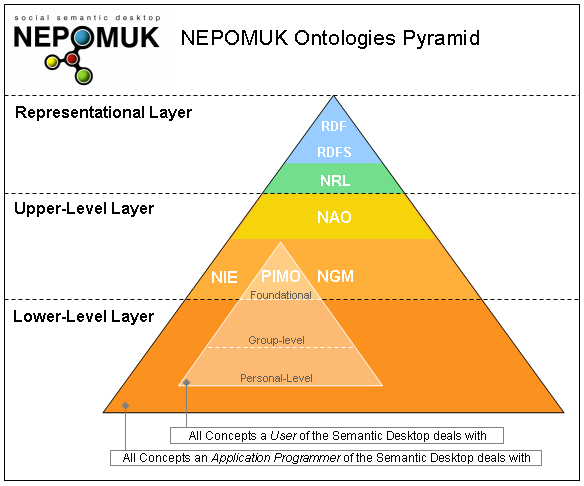
\includegraphics[width=1.00\textwidth]{images/roadmap.png}
	\caption{Integrated Ontologies}
	\label{fig:roadmap}
\end{figure}

The NEPOMUK Representational Language \textbf{NRL ontology}\footnote{\url{http://www.semanticdesktop.org/ontologies/nrl/}} builds the representational layer and the semantic
metadata axioms used to express PIMO. 
NRL is a meta-language comparable to OWL or RDF/S. 
The key characteristics of NRL are (on top of RDF/S) support for named graphs
in semantic statements, a notation for contextualized inference and semantics, 
and a selection of semantic relations (inverse, transitive, reflexive).

The NEPOMUK Information Element \textbf{NIE ontology}\footnote{\url{http://www.semanticdesktop.org/ontologies/nie/}} describes desktop elements such as address book entries, documents,
e-mails, appointments, pictures, and multimedia files.
The ontology discriminates between the representation (binary files)
and the information stored therein. 
PIMO reuses the classes of NIE and suggests how to integrate
and annotate vast personal spaces of information (PSI) expressed in NIE.

Annotations and tagging are represented in the NEPOMUK Annotation \textbf{NAO ontology}.
It represents change-dates, author, and other key metadata of documents.
NIE and PIMO both extend NAO. A part of NAO is the NEPOMUK Graph Metadata \textbf{NGM ontology} to annotate named graphs.

The PIMO ontology crosses two of the layers in the ontology pyramid, data related to PIMO can be divided into three smaller layers (also visible in Figure\ref{fig:roadmap}):
\begin{itemize}
	\item \emph{Foundational PIMO}: The PIMO ontology as such, as defined in this specification and accompanying NRL serialization. This includes the classes and properties of \emph{PIMO-upper} (see Section \ref{sec:pimoupper}), which work on the \emph{Upper-Level Layer} of NEPOMUK and everything else defined in the PIMO vocabulary. PIMO-upper is the same for every Semantic Desktop user and is valid in a global context.
	\item \emph{Group-level PIMO}: Domain ontologies that are shared within a group. They can be imported by users. A description is given in Section~\ref{sec:pimomid}.
	\item \emph{Personal-level PIMO}: The classes, properties, and Things created by an individual user. Also called \emph{user-PIMO}, this layer includes the data that is only relevant in the context of one individual.
\end{itemize}

\section{Examples}
\label{sec:examples}
A scenario is used to explain the ontology elements. A fictional persona, Claudia Stern, is our example user. She is working for EX-Ample Inc., a fictional company producing ``\textbf{Ex}treme Guitar \textbf{Ampl}ifi\textbf{e}rs'', and her current task is to organize a business trip to a meeting with guitarists and bass players in Belfast.

% taken from RDFS primer
For convenience and readability, this specification uses an abbreviated form to represent URI-References. A name of the form \texttt{prefix:suffix} should be interpreted as a URI-Reference consisting of the URI-Reference associated with the prefix concatenated with the suffix.

RDF graphs are written in N3/Turtle syntax. Examples serialized as RDF appear in this typesetting:
%\note{\emph{Knud}: I find the statement (Claudia user Claudia) very confusing. What's that supposed to mean? \emph{Leo}: that was garbage, we had it in the ontology before as an alternative to isDefinedBy.}
{\small
\begin{verbatim}
claudia:Claudia a pimo:Person;
 pimo:isDefinedBy claudia:PIMO;
 nco:hasEmailAddress <mailto:claudia@example.com> .
\end{verbatim}
}

\subsection{PIMO ontology and namespaces}
The ontology described in this document has this namespace:

{\small
\begin{verbatim}
Namespace:
http://www.semanticdesktop.org/ontologies/2007/11/01/pimo#
\end{verbatim}
}

During the lifetime of the NEPOMUK project (until Dec 2008), the PIMO ontology
and the according documentation may change, but the namespace will not change.
The namespace stays fixed to keep the necessary changes
of software implementations at a minimal level.
We have adopted this practice from other projects, which have applied it successfully. Examples are the W3C's  XSD datatypes (the recommendation changed in 2007, the namespace did not) or the FOAF project.

Throughout this document these ontologies and namespaces are used, also indicating their respective versions PIMO is building on:
{\small
\begin{verbatim}
@prefix rdf:  <http://www.w3.org/1999/02/22-rdf-syntax-ns#>.
@prefix rdfs: <http://www.w3.org/2000/01/rdf-schema#>.
@prefix nrl:  <http://www.semanticdesktop.org/ontologies/2007/08/15/nrl#>.
@prefix nao:  <http://www.semanticdesktop.org/ontologies/2007/08/15/nao#>.
@prefix pimo: <http://www.semanticdesktop.org/ontologies/2007/11/01/pimo#>.
@prefix ncal: <http://ont.semanticdesktop.org/ontologies/2007/04/02/ncal#>.
@prefix nco:  <http://ont.semanticdesktop.org/ontologies/2007/03/22/nco#>.
@prefix nfo:  <http://ont.semanticdesktop.org/ontologies/2007/03/22/nfo#>.
@prefix nie:  <http://www.semanticdesktop.org/ontologies/2007/01/19/nie#>.
@prefix nmo:  <http://www.semanticdesktop.org/ontologies/2007/03/22/nmo#>.

@prefix claudia: <http://www.example.com/people/claudia#> .
\end{verbatim}
}

\section{Creating Personal Information Models}
\label{sec:creatingPIMOs}
In this section, all key elements of the ontology are presented.
The order used reflects the steps a knowledge engineer will have to take to implement this recommendation.

\subsection{The User and their Individual PIMO}
\label{sec:pimo-user}
As a prerequisite to create a PIMO and Things inside the PIMO, each user needs a \emph{personal namespace}. The namespace is used as a prefix for all URIs minted for the user. Often these are namespaces using the HTTP URI scheme, but any RDF namespace can be used. The example namespace used in this document is \texttt{http://www.example.com/people/claudia\#} and is abbreviated with ``\texttt{claudia:}''.

\note{\emph{Knud}: In general, I would write all ontology elements in a different font. E.g., \texttt{pimo:Person}
\emph{Leo}: actually, I would like to write a script that, once this is converted
to HTML, replaces all ``pimo:NAME'' with HTML links to the ontology definition 
within the namespace.
\emph{Knud, 28/12:} unfortunately, there isn't always a namespace given. For now, I changed all ontology elements to monospaced font}

Users are represented as instances of the class \texttt{pimo:Person}. For each instance, a new URI is generated and a few key facts are represented to identify the user.
After the user has been instantiated, details such as email addresses are added by using terms from the NEPOMUK contact ontology, NCO. 
%\note{Knud: What do you mean by ``as the second object''? \emph{Leo}: fixed this, its a new resource.} 
In NCO, contact information connected to people is modeled as a complex resource, not as a simple literal:
%For the sake of simplicity, we used the URL \texttt{mailto:claudia@example.com} as identifier for this nco:EmailAddress resource.
{\small
\begin{verbatim}
claudia:Claudia a pimo:Person;
 rdfs:label "Claudia Stern";
 nco:hasEmailAddress mailto:claudia@example.com.

mailto:claudia@example.com a nco:EmailAddress;
 nco:contactMediumComment "work";
 nco:emailAddress "claudia@example.com".
\end{verbatim}
}

The second entity that needs to be represented is the \emph{Personal Information Model of the User}. It is connected to the user via the \texttt{pimo:creator} relation, and the user's namespace is added.
For Claudia this is:

{\small
\begin{verbatim}
claudia:PIMO a pimo:PersonalInformationModel;
  pimo:creator claudia:Claudia;
  nao:hasDefaultNamespace "http://www.example.com/people/claudia#";
  nao:hasDefaultNamespaceAbbreviation "claudia".
\end{verbatim}
}

\texttt{pimo:PersonalInformationModel} is a sub-class of \texttt{nrl:Ontology}, allowing more metadata to be added using NRL compliant standards. More about NRL metadata is described in Section~\ref{sec:nrlgraphs}. 
We further call a this instance of \texttt{pimo:PersonalInformationModel} of an individual a \emph{user-PIMO}. Claudia's user-PIMO is \texttt{claudia:PIMO}. As an abbreviation, it is also correct to write  ``Claudia's PIMO'' instead of ``Claudia's user-PIMO''.
\note{\emph{Knud, 28/12:} I'm confused by this term PIMO-user. It sounds as if it meant ``The user of the PIMO'', but it actually means ``The PIMO of the user'' --- correct? That's potentially confusing.} 
\note{\emph{Leo, 8/1:} reduce to ``user's PIMO'' and ``Claudia's PIMO''?}

\subsection{Things}
\label{sec:thing}
The PIMO ontology defines the basic class \texttt{Thing} for mental concepts. Every information element encountered in knowledge work by a user is represented as a Thing.
\note{\emph{Knud, 28/12:} Thing is inconsistently spelled with lower- and upper-case throughout the document.}
A Thing is a unique representation of an entity of the real world within one user-PIMO. On the PSI of a user, a real world entity can be represented in multiple data sources. For example, the person ``Dirk Hagemann'' may be author of an e-mail, described in an address book entry, and stored in a accounting tool, all part of the workspace of ``Claudia''. 
One instance of \texttt{pimo:Person} is created as unique \texttt{Thing} linking to these multiple representations, such as shown in Figure~\ref{fig:thing_vs_resource}.
\note{\emph{Knud, 28/12:} Yes, this is a Thing, but it is also a pimo:Person? Potentially confusing. \emph{Leo, 8/1:} changed the wording to speak of a Person}

\begin{figure}[htbp]
	\centering
		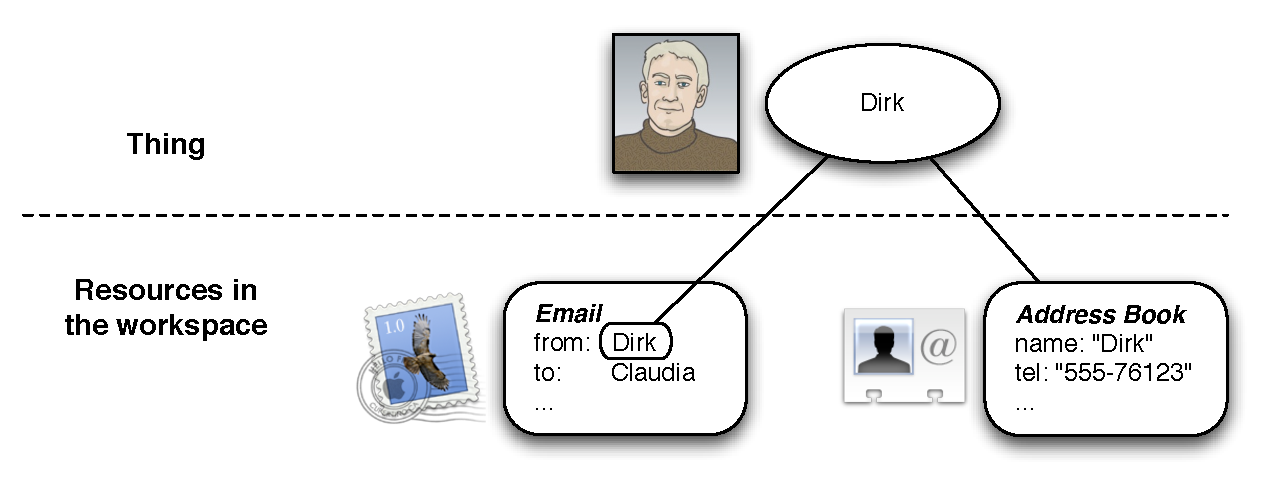
\includegraphics[width=1.00\textwidth]{images/thing_vs_resource}
	\caption{Thing and Resources}
	\label{fig:thing_vs_resource}
\end{figure}

An application handling a resource in the workspace can be aware that there may be a Thing representing the resource. For example, Claudia's e-mail client may examine the sender of an e-mail (Dirk) and search for the \texttt{pimo:Thing} that represents Dirk uniquely. Once the right Thing is found by the application, more information about Dirk can be discovered.

This principle includes all elements (\texttt{nie:InformationElement} and other RDF resources) in the user's \emph{Personal Space of Information (PSI)}. 
For each information element, a Thing in the user's PIMO must be created. 
The information element exists independent of the user, the same element can
be stored in multiple folders or data sources on one desktop, and also on other desktops and on the web. 
A Thing is the personalized view of \emph{one user} on this information element, independent of representation or storage location.

To be adequate, a PIMO of a user should contain all nameable entities known to the user,
but to be efficient, this representation should be restricted to the minimal data needed.
%Leo 29.7.2008: this is also explained later
% Identification is part of this minimal data, and \texttt{nao:identifier} provides the property for it.

\subsection{Connecting Things to the User's PIMO}
\label{sub:connectingThingsToPimo}
In a scenario of multiple connected semantic desktops, it will frequently occur that users import data from each other's desktop onto their own desktop.
It is therefore important to know which resources (primarily Things, but also Classes and Properties) were created by which user and originate from which PIMO. For this, the property \texttt{pimo:isDefinedBy} is used.

Continuing the example above, this property connects the Person to the PIMO in which it is defined.  This is mandatory for every defined Thing and allows applications to identify which elements are part of a user-PIMO and which are not\footnote{We intentionally did not only rely on NRL graphs to model the relation between the model and instances defined by it. A graph can only contain \emph{statements}, 
about, but not \emph{resources} as such.
To model that a resource is part of a PIMO, the \texttt{pimo:isDefinedBy} relation is a clear representation.
Additionally, named graphs can be used to declare what \emph{statements} are declared in a PIMO, see~\ref{sec:nrlgraphs}}.

{\small
\begin{verbatim}
claudia:Claudia pimo:isDefinedBy claudia:PIMO.
\end{verbatim}
}

An \texttt{isDefinedBy} property is also defined in RDFS, where resources can be connected to their defining ontologies, and is also discussed in the light of the OWL standard\footnote{\url{http://www.w3.org/2007/OWL/wiki/Syntax\#Declarations_and_Structural_Consistency}}. 
The semantics of \texttt{isDefinedBy} in PIMO is based on these, with the extension that we define it as a required property.

\subsection{Identification of Things}
\label{sec:identification}
A Thing \textbf{must} have an URI and \textbf{should} be described with properties that identify it. 
Identifiers allow to analyse information elements and find occurrences of the Thing.
For example, the person ``Dirk Hagemann'' is represented once as an instance of the class \texttt{pimo:Person} and identified using his e-mail address. 
The RDF descriptions of emails and documents can then be analysed to find resources that represent the same entity via this identifier. 
{\small
\begin{verbatim}
# The canonical Dirk
claudia:DirkHagemann a pimo:Person;
 pimo:isDefinedBy claudia:PIMO;
 nco:hasEmailAddress <mailto:dirk@example.com>.

# An e-mail in which Dirk #2 occurs
<imap://claudia@example.com/INBOX/1> a nmo:Mail;
 nmo:from <imap://claudia@example.com/INBOX/1#from>.

# Dirk #2, the email sender
<imap://claudia@example.com/INBOX/1#from> a nco:Contact;
 nco:hasEmailAddress <mailto:dirk@example.com>.
<mailto:dirk@example.com> a nmo:EmailAddress;
 nco:emailAddress "dirk@example.com".
 
# Dirk #3, as address book contact
<file://home/claudia/dirk.vcf#dirk> a nco:PersonContact;
 nco:nameFamily "Hagemann";
 nco:nameGiven "Dirk";
 nco:hasEmailAddress <mailto:dirk@example.com>;
 nco:photo <http://www.example.com/people/dirk/photo.jpg>.
 
\end{verbatim}
}

In this example, we see that the Person Dirk appears three times in this knowledge workspace. First, in the form of an instance of \texttt{pimo:Person}, as the canonical Dirk. Second, as sender of an e-mail and third as entry in an address book. Only one instance is the \texttt{pimo:Thing} representation of Dirk: \texttt{claudia:DirkHagemann}. The others are information elements representing the same entity.

\begin{figure}[htb]
	\centering
		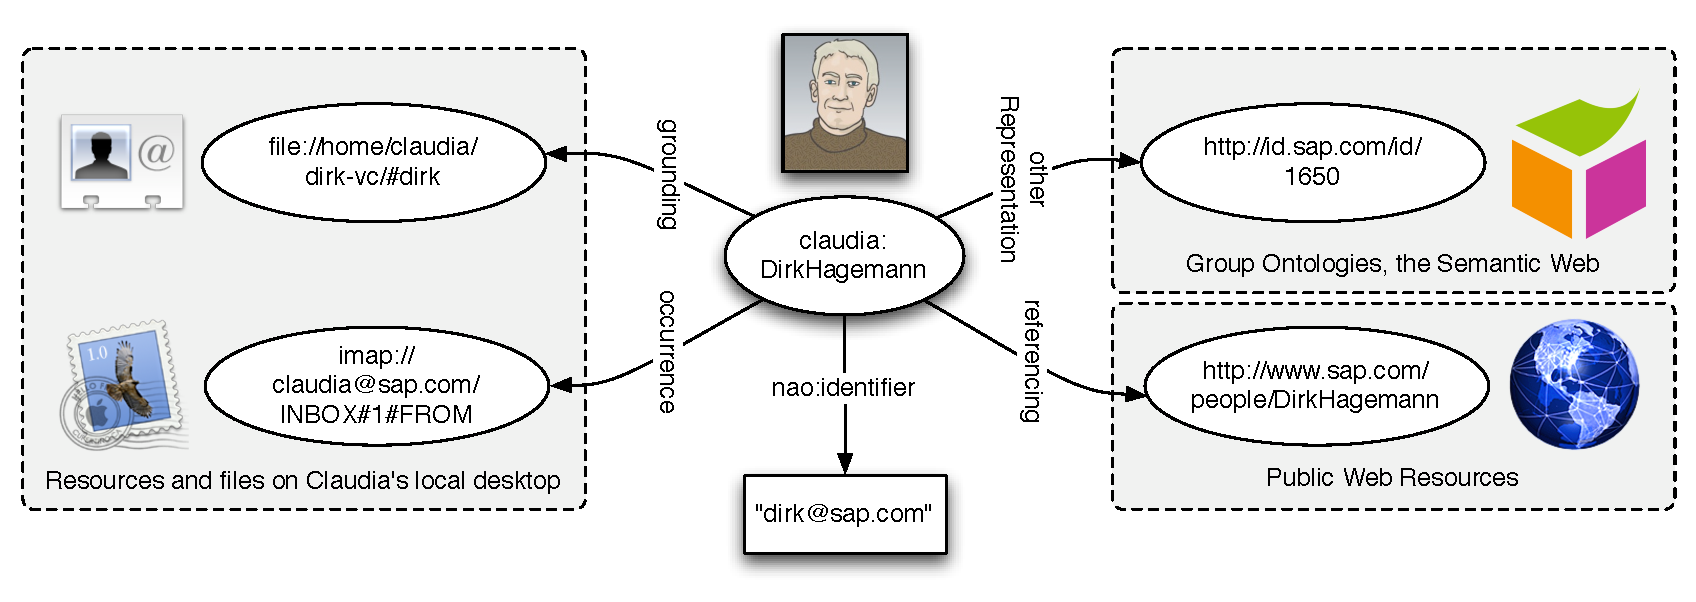
\includegraphics[width=1.00\textwidth]{images/identification}
	\caption{Different Identification Mechanisms}
	\label{fig:identification}
\end{figure}


%\note{\emph{Knud}: can one ``use'' an assumption? Leo: rephrased to ``is based on''}
To work effectively, PIMO is based on the \emph{Unique Name Assumption} (UNA). 
The UNA is a rule that declares two RDF resources with different URIs as different individuals. 
This is common in desktop applications (for example files with different names are different) and intuitive to grasp for users. But it is different from the OWL ontology language
%\note{\emph{Knud}: is OWL a system? Leo: its an ontology language}
where duplicate entries are common and the UNA is not enforced. 
PIMO is designed for personal systems, where an application has access to the complete model and can avoid duplicates before creating them.

To enforce the UNA, duplicate Things \textbf{must} be avoided. 
The crucial moment to do this is before creating a new Thing.
Things can either be created by the user manually or automatically by analysing existing native resources. In any case, before creating a new Thing, all existing Things have to be examined if a Thing with a same name or same identifying properties already exists. 
If an existing Thing is found, it \textbf{must} be reused. 
Immediately after creating a new Thing, identifying properties should be set to distinguish the Thing and avoid duplication. 
% fix to https://dev.nepomuk.semanticdesktop.org/ticket/498
Section \ref{sec:creatingthingalgorithm} further describes the complete process of creating things.

In the next paragraphs, essential identifying properties are described, an overview is given in Figure~\ref{fig:identification}.

\textbf{The primary identifier of a Thing is it's URI}. New URIs for Things \textbf{must} be generated using the namespace of the user as prefix and then a unique local name. 
Although the local name can be entirely a random string, we recommend to include the label in the URI for readability. When minting a new URI that clashes with an existing URI, a random element can be added to the new URI. A URI for Claudia Stern is:
\begin{verbatim}
claudia:Claudia
\end{verbatim}

\paragraph{NAO-Identifiers} Existing identification schemes based on NAO should be reused for this purpose by representing them with 
%\note{Knud: you say pimo:identifier here and nao:identifier in the example below. Which one is it?\emph{Leo}: its nao:identifier (28.8.2007).} 
\texttt{nao:identifier} and its sub-properties. 
If an identifier is found as meta-data of a native resource (usually an \texttt{nie:InformationElement}), the identifier \textbf{must} be copied to the Thing.
This allows others to match and identify the correct Thing when encountering the next information element.
Example identifiers are \texttt{nmo:messageId} for e-mails, \texttt{ncal:uid} for appointments, or \texttt{nexif:imageUniqueID} for images. 
Instead of using the plain \texttt{nao:identifier} property, these specific properties should be used or new sub-properties of \texttt{nao:identifier} created
\footnote{I.e. if you want to represent ISBN numbers and there is no property for them, create a new sub-property \texttt{isbn} of \texttt{nao:identifier}.}.
In this document, we assume that e-mail addresses can be used to identify persons.

\note{\emph{Leo}: this example is not good, as e-mail addresses are modeled 
differently in NCO. How else can we identify a person? \emph{Knud, 28/12:} I think we can't... :P}
\begin{verbatim}
# Copy all identifiers you can find about the Thing.
claudia:DirkHagemann a pimo:Person;
 nao:identifier "dirk@example.com".
\end{verbatim}

Identifiers consisting of multiple RDF statements cannot be captured using \texttt{nao:identifier}.
They are comparable to a primary key in a relational database consisting of multiple
columns. These \textbf{multi-key identifiers} \textbf{must} be merged into one \texttt{nao:identifier}.

\paragraph{Grounding Occurrence} The relation \texttt{pimo:groundingOccurrence} is used to link a Thing to an \texttt{nie:InformationElement} that has this Thing as primary topic. For example, the grounding for a person could be the entry in the address book describing the person. On the other hand, an e-mail with this person as the sender or recipient would normally not be a grounding occurrence. A Thing represents the mental concept, the \texttt{pimo:groundingOccurrence} links to existing Information Elements that are handled by existing applications. This is a key for reusing the features of these applications. 
The grounding occurrence can change, for instance if a file was moved and the URI of the Information Element changed, the grounding occurrence relation needs to be changed. 
A similar case happens when a file is uploaded to a shared workspace and not kept locally any more --- all annotations of the Thing stay the same (the URI of the Thing does not change), the Information Element changes.
Multiple values are allowed, this reflects the fact that the same Thing can be represented in multiple applications, and dependent on the work context, the user may want to open a different application. 
{\small
\begin{verbatim}
# Link to Dirk #3 from example above.
claudia:DirkHagemann a pimo:Person;
 pimo:groundingOccurrence <file://home/claudia/dirk.vcf#dirk>.
\end{verbatim}
}
\paragraph{Occurrence} The relation \texttt{pimo:occurrence} connects a \texttt{pimo:Thing} with a resource representing the same real world entity.
Facts about the occurrence are then also valid for the connected Thing. 
For example, if the person Dirk appears as sender of an e-mail, then the resource identifying the sender is an \emph{occurrence} of Dirk. 
Based on the occurrence relation, Dirk (the unique \texttt{pimo:Person}) is the sender of the given e-mail.
Occurrence relations are to be used on resources \emph{representing} the same entity in a different context, but not on resources \emph{mentioning} the entity. For example, it is not valid to say that an e-mail is an occurrence of a person, only the sender or recipient can be occurrences of a person.

%Not the e-mail as such is the occurrence, but the sender within. 
\note{\emph{Knud, 28/12:} Why is the e-mail as such not the occurrence? This should be explained, or not mentioned at all. 
Leo: done, removed sentence, replaced with longer explanation.}
Occurrences of a Thing can be found by searching for entities with the same identifying properties.

{\small
\begin{verbatim}
# Link to Dirk #2 from example above, 
# he occurs as sender of an e-mail
claudia:DirkHagemann a pimo:Person;
 pimo:occurrence <imap://claudia@example.com/INBOX/1#from>.
\end{verbatim}
}

Besides identification, both the \texttt{pimo:groundingOccurrence} and the \texttt{pimo:occurrence} relation have 
implications on data integration and affect semantic meaning of a Thing. 
This will be described later in Section \ref{sec:pimoVSnie}.

\paragraph{Referencing Occurrence} 
%\note{Maybe rename to indicatingOccurrence, closer to Topic Maps? Leo: I don't care, leave it as is.}
\label{par:referencingOccurrence}
A Referencing Occurrence is an indirect approach to identification. 
Annotating a Thing with an information element as \emph{referencing occurrence} states that the information element contains a description of the Thing.
Its primary topic must be the Thing.
The Thing is indirectly identified by the element, when two Things in different models share the same information element as referencing occurrence, they may be equal and could be matched. 
The following description is an adaption of XTM's subject indicators~\cite{XTM,Rath2003}.
The referencing occurrence is a kind of proxy for the Thing. Examples of referencing occurrences are:

{\small
\begin{verbatim}
claudia:DirkHagemann a pimo:Person;
 pimo:referencingOccurrence <http://www.example.com/people/DirkHagemann>.
 
claudia:ExampleInc a pimo:Organization;
 pimo:referencingOccurrence <http://www.example.com/>;
 pimo:referencingOccurrence <http://en.wikipedia.org/wiki/Example.com>.
\end{verbatim}
}

It should contain a human readable documentation describing the concept. The resource could be a document, ontology, video, audio, anything able to describe to a human what the concept is about. The resource is a reference to the concept of the Thing. 
A good example for a referencing occurrence is a wikipedia article.

A referencing occurrence describes the concept with the purpose of being widely used by ontologies. Consequently, it is important that the document describes exactly what concept it is about and what not. Even if the author works as accurately as possible, different people will never interpret a referencing occurrence 100\% the same way. However, the concept of referencing occurrences is worth using it, because it allows a shallow match of heterogenous information models, and because there is finally no alternative to it. 

\textbf{It is recommended to use wikipedia URIs as objects of referencing occurrences.} In contrast, URIs minted by \emph{DBPedia}\footnote{DBPedia is a Semantic Web representation of wikipedia and provides URIs for concepts, whereas wikipedia provides URIs for documents describing concepts. An example DBPedia URI is: \url{http://dbpedia.org/page/Berlin}} \textbf{must} be related using the \texttt{pimo:hasOtherRepresentation} relation.

\paragraph{Other Representation} 
\label{par:otherRepresentation}
The \texttt{pimo:hasOtherRepresentation} relation is used to connect \texttt{pimo:Things} with other representations of the same Thing in other Semantic Web ontologies. 
This can be the case with shared ontologies, such as company white page systems or Semantic Social Networking websites. 

The knowledge modeled should be compatible with the ontologies used by the user. An example for such other representation is\footnote{Using the URI scheme of the ECS University in our example domain. \url{http://id.ecs.soton.ac.uk/docs/}}:
\begin{verbatim}
claudia:DirkHagemann a pimo:Person;
 pimo:hasOtherRepresentation <http://id.example.com/person/1650>.
\end{verbatim}

Another example would be the city of Belfast where Claudia wants to travel to,
linked to the DBPedia entry about it:
\begin{verbatim}
claudia:Belfast a pimo:City, pimo:Tag;
  pimo:isDefinedBy claudia:PIMO;
  pimo:tagLabel "Belfast";
  pimo:hasOtherRepresentation <http://dbpedia.org/resource/Belfast>;
  geo:lat "54.5833333";
  geo:long "-5.9333333".
\end{verbatim}
The relation can be used both to identify Things by their other representations,
and to fetch more data.
In this example, the latitude and longitude are actually superfluous data,
as they can be retrieved from the other representation
in DBPedia.
Assuming Dirk also represents Belfast in his PIMO, but independent from Claudia,
but linking to the same DBPedia entry, algorithmically matching their different representations is straightforward.

\paragraph{Other Conceptualization}
To map user-generated classes to classes defined in other ontologies, the 
\texttt{pimo:hasOtherConceptualization} relation connects classes defined in a user's PIMO
with classes defined in domain ontologies. 
Classes defined in domain ontologies should be sub-classes of PIMO-upper classes, see Section \ref{sec:integratingontologies}. 

Implementations can use the \texttt{pimo:hasOtherConceptualization} to allow the user and algorithms
to map user--specific classes to classes defined in other ontologies,
without implying that there is a sub-class relationship.

\subsection{A Complete Example} 
A complete example for all different identification properties 
can now be built from the above annotations.

For Claudia, her co-worker Dirk Hagemann is identified and linked to occurrences like this:

{\small
\begin{verbatim}
# The canonical pimo:Person Dirk, 
# a pimo:Thing from Claudia's PIMO
claudia:DirkHagemann a pimo:Person;
 pimo:isDefinedBy claudia:PIMO;
 nao:prefLabel 'Dirk Hagemann';
 nao:identifier "dirk@example.com";
 pimo:occurrence <imap://claudia@example.com/INBOX/1#from>;
 pimo:groundingOccurrence <file://home/claudia/dirk.vcf#dirk>;
 pimo:referencingOccurrence <http://www.example.com/people/DirkHagemann>;
 pimo:hasOtherRepresentation <http://id.example.com/person/1650>.
 
 
# An e-mail in which Dirk #2 occurs
<imap://claudia@example.com/INBOX/1> a nmo:Mail;
 nmo:from <imap://claudia@example.com/INBOX/1#from>.

# Dirk #2, as email sender
<imap://claudia@example.com/INBOX/1#from> a nco:Contact;
 nco:hasEmailAddress <mailto:dirk@example.com>.
 
<mailto:dirk@example.com> a nmo:EmailAddress;
 nco:emailAddress "dirk@example.com".
 
# Dirk #3, as address book contact
<file://home/claudia/dirk.vcf#dirk> a nco:PersonContact;
 nco:nameFamily "Hagemann";
 nco:nameGiven "Dirk";
 nco:hasEmailAddress <mailto:dirk@example.com>;
 nco:photo <http://www.example.com/people/dirk/photo.jpg>.
\end{verbatim}
}

This allows implementations to:
\begin{itemize}
	\item identify the Thing when found occurring in documents,
	\item open a grounding occurrence to see the Thing within an existing desktop application (i.e. the address book entry for a person),
	\item match this Thing with other representations via the same referencing occurrence,
	\item use the other representation from the company's white pages to show additional data about the Thing.
\end{itemize}

The \texttt{pimo:occurrence} link is the generic basis, \texttt{pimo:groundingOccurrence} and \texttt{pimo:hasOtherRepresentation} are sub-properties of it. This data should be generated automatically and unsupervised. 
Adding identifying properties to a Thing helps to find more occurrences and therefore more information about it.

\subsection{Labels and Names of Things}
\label{sec:labelling}
To label Things, we recommend the NEPOMUK Annotation Ontology (NAO) vocabulary
and extended it.
NAO defines properties for the \emph{preferred label}, \emph{multiple alternative labels}. PIMO defines \emph{tag labels} as unique names for unique Tags.

\paragraph{\texttt{nao:prefLabel}} \textit{A preferred label for a Thing}.
This property \textbf{must} be applied to every instance of \texttt{pimo:Thing} (or its sub-propery \texttt{pimo:tagLabel}).
It can be used by applications to represent the Thing with a textual label and should be human-readable. There must only be one \texttt{prefLabel} per Thing (mincardinality and maxcardinality should be one)\footnote{These restrictions are not explicitly noted in the RDF description of the property, as NRL does not support property restrictions for classes.}.

\paragraph{\texttt{pimo:tagLabel}} \textit{Defines a unique personal label for a Thing, which then is also a Tag.}
The label \textbf{must} be unique within
the scope of a user. 
If both are set, \texttt{pimo:tagLabel} and \texttt{nao:prefLabel} of a resource \textbf{must} have the same value. 
It is a sub-property of \texttt{nao:prefLabel} and of \texttt{nao:personalIdentifier}.

\textbf{Tag labels are the \textbf{recommended} way to label and identify Things that are used for classification}.
As they are unique and human-readable, they \textbf{may} be used for multiple application scenarios such as wikis, tagging, or matching terms found in free-text.
Naming a Thing with a \texttt{pimo:tagLabel} gives the Thing a second type, \texttt{pimo:Tag}, which indicates that the Thing should now be considered part of the user's tagging system, see Section~\ref{sec:tagginginpimo}. 
\note{\emph{Knud, 28/12:} I don't understand: should the two properties be the same or not? Leo: recommended they should be the same.}

\paragraph{\texttt{nao:altLabel}} \textit{An alternative label alongside the preferred label for a Thing.} These are alternative spellings, translations, nick-names.
%\note{\emph{Knud, 28/12:} Spelling Mistakes? Leo: removed this, replaced with nick-names}
Implementations can use these labels to find Things when the user enters a text in a search box or when analysing free text.
If a Thing has occurrences, the labels of occurrences \textbf{should} be copied as alternative labels to the thing.

In combination, these labelling techniques allow applications to clearly label Things in user interfaces but also to lookup for Things based on alternative names. For our example, these are:

\begin{verbatim}
claudia:DirkHagemann a pimo:Person;
# preferred label when shown
 nao:prefLabel "Dirk Hagemann";
# a nickname for Dirk
 nao:altLabel "hacki";
# a common misspelling
 nao:altLabel "Dirck Hagemann";
# the personal identifier and tag label, 
# Attention: this requires the class pimo:Tag
 pimo:tagLabel "Dirk Hagemann".
\end{verbatim}

Additionally, visual cues (icons, images, thumbnails) can be attached by using NAO symbol relations:
\begin{itemize}
	\item \texttt{nao:hasSymbol}
	\item \texttt{nao:prefSymbol}
	\item \texttt{nao:altSymbol}
\end{itemize}

\subsection{Textual description of Things}
\label{sec:freetextdescription}
To describe Things with a free-text, the simple \texttt{nao:description} property should be used. This allows users to add a (possibly searchable) description of the Thing in a simple way. The description string value should contain no format markup but be a plain text.

For more complex free-text descriptions of Things, the property \texttt{pimo:wikiText} is reserved. 
Formatting (font-weight, italics) and linking to other pages is supported
in this property, implementers may use the \emph{Wiki Interchange Format}
\footnote{\url{http://semanticweb.org/wiki/Wiki_Interchange_Format}}
as syntax, or RDFa\cite{rdfaprimer}.

\subsection{Rating and Ranking Things} % (fold)
\label{sec:ratings}
\textbf{Ratings of Things} can be expressed using \texttt{nao:numericRating}.
For numericRating, the range of values \textbf{must} be within $[0..10]$ (inclusive)
\footnote{Implementers may wonder why the range is not standardized as $[0..1.0]$. The recommended range is based on an implementation decision taken in KDE.}. 
A value of '0' is interpreted as not set, a rating of 1 a \emph{bad rating} and a rating of 10 a \emph{good rating}. 
Furthermore, resources can only be given at most one numeric rating, thus the maximum cardinality is 1.
Applications \textbf{may} partition the values into discrete ratings (such as 2, 4, 6, 8, 10 to represent the semantics of ``5 star ratings'').

The rating values may and should be used for \emph{ranking} of Things
and filtering. A populated PIMO contains thousands of Things,
user interfaces should use the \texttt{nao:numericRating} values
to filter out low-ranked resources and highlight high-ranked
resources.
Implementations \emph{can} set the \texttt{nao:numericRating} 
values automatically to computed values.
% Alternatively, implementations can set an automated rank and
% compute the overall rank using auotmated rank + nao:numericRating


% paragraph ratings (end)

\subsection{Modelling Time}
In PIMO, no special treatment of time is modeled. 
We are aware that representing points in time, durations, and other periods of time
is an important aspect of ontologies. 
We recommend to use the XML Schema Datatypes
to represent time. 
There, ISO 8601 is recommended. Timezones must be handled according to this standard,
encoded inside the literal value\footnote{For a detailed representation of time events, refer to the NIE documentation, where timezones are discussed (\url{http://www.semanticdesktop.org/ontologies/2007/04/02/ncal/\#sec-tzd}).
NIE represents time using the NcalDateTime class and its properties 
date, dateTime, ncalTimezone. Timezones are represented using a Timezone class,
that is inspired by RFC 2445.}.

Periods of time can be represented using sub-classes of the abstract class
\texttt{pimo:ProcessConcept} which represents lasting processes such as events
or projects. For durations that last a number of days or months, we recommend to use the standardized XML datatypes\footnote{The XS namespace is \texttt{http://www.w3.org/2001/XMLSchema}, but the two duration datatypes are defined in the XPath recommendation in 2007, see \url{http://www.w3.org/TR/xpath-functions/\#dt-dayTimeDuration}}:
\begin{itemize}
	\item \texttt{xs:dayTimeDuration} for durations measured in days, hours, and minutes.
	\item \texttt{xs:yearMonthDuration} for durations measured in months and years
\end{itemize}
Implementers are free to use either the XSD types or sub-classes of 
\texttt{pimo:ProcessConcept}.

There have been issues with other notations of duration and therefore the W3C Semantic Web Best Practices and Deployment Group published a note\footnote{\url{http://www.w3.org/TR/swbp-xsch-datatypes/\#section-duration} Since XPath 2.0 has become a W3C recommendation in January 2007, this note is partly obsoleted.} to restrict durations to these values. 

\subsection{Representing Modification and Change Dates}
\label{sec:changedates}
The change and creation dates of Things are important metadata for personal information management applications. Knowing about recent changes is an important cue for users to retrieve documents. Many applications offer the feature to show recent changes or filter by them. Consequently, it has to be straightforward, simple, and fast to query for the modification dates. 

The NAO properties \texttt{nao:created}, \texttt{nao:modified}, and \texttt{nao:lastModified} \textbf{shall} be used to track the change dates of Things. 
Creation and modification allow only one, modification allows multiple date values.
Created and lastModified values \textbf{must} be set for each Thing,
at least one modified value \textbf{must} be set.
These values are intended for resources of type \texttt{pimo:Thing}, \texttt{pimo:Association}, \texttt{rdfs:Class}, and \texttt{rdf:Property} when created by the user.
\note{\emph{Knud, 28/12:} Why is this not enforced? 
\emph{Leo, 8/1:} mandatory is better anyway, CHANGED}

Example:
\begin{verbatim}
# Represent modification dates of a Thing
claudia:DirkHagemann
  nao:created "2007-10-26T15:23:01";
  nao:modified "2007-10-26T15:23:01";
  nao:modified "2007-10-29T08:04:30";
  nao:lastModified "2007-10-29T08:04:30".
\end{verbatim}

The \textbf{semantics} of these dates is that the description of the Thing has changed, facts about the Thing have been added, removed, or modified. Changes to \texttt{pimo:objectProperty} (\texttt{pimo:related}, \texttt{pimo:hasTag}, etc.) or \texttt{pimo:datatypeProperty}  (\texttt{name}, \texttt{address}, \texttt{label}, etc.) imply such a modification. 
Included are also changes to the labels (\texttt{nao:prefLabel}, \texttt{nao:altLabel}, \texttt{pimo:tagLabel}).
Modification of any other statement (such as \texttt{pimo:definedBy}, \texttt{nao:modified}) do not imply a modification nor a change of dates.
As current RDF stores a priori do not support automatic tracking of changes, applications have to implement housekeeping of these dates, or use services for tracking.
\footnote{The value of lastModified is redundant as it could be computed by sorting the modified dates during query time, but this is not possible without nested SPARQL queries, a $max()$ function, and grouping, none of these part of the SPARQL standard. The stores that support such non-standard operations still need time to compute the value. As the last modification date is very important for applications to assist users finding information, the redundancy is intended.}

\note{\emph{Knud, 28/12:} I removed a paragraph here (still commented in the source), because I think it doesn't belong here. This document is a specification, not a scientific document. Leo: OK}
%In RDF and using named graphs, there are more ways of representing change dates. It is possible to remember the date when a graph changes, implying that all triples inside the graph have changed. Based on this, it can be implied that all resources described in these triples have changed. But there is no formal relation between a resource and a graph that describes it. For example a class being used as object of a rdf:type relation, does this express that the class has changed? Or a resource being annotated in a reification statement. Changes to the graph may not directly relate to changes of the resource in the view of the user. 
%Also, as dates are a very prominent fact needed for data visualization and search result ranking, a graph-based approach will not provide satisfactory answer times
%\footnote{To select a date using graph metadata, a query for the context of all statements where a resource is either in subject or object role and the change date of these contexts would be needed.}.

\subsection{Setting the Class of a Thing}
\label{sec:classofthing}
All Things are of type \texttt{pimo:Thing} or one of its sub-classes. The PIMO ontology itself defines several sub-classes such as \texttt{pimo:Person} or \texttt{pimo:Organization}. If these are not specific enough, the user can either create new sub-classes manually (see Section \ref{sec:customontology}), or import group-level ontologies (Section~\ref{sec:integratingontologies}).

As a rule of thumb, the question to be answered by assigning the class is ``\emph{What is this Thing?}''.
In comparison to OWL, where classes are commonly based on the properties of the object (``vegetarians are entities not eating flesh'') , classes represent the type (the \emph{nature}) alone. 
\note{\emph{Knud, 28/12:} idea: paragraphs such as this should be marked as ``suggestion for use''. Again, they don't really belong in a specification.
\emph{Leo, 8/1:} This paragraph is explanatory of the idea of classes in comparison to OWL, where most things are modeled as ``does this thing belong to a class or not'' Its important to have it. Cutted it, reworded it to refer to OWL. DONE?}
%For the concrete example of ``importance'', we recommend using the property \texttt{nao:numericRating} or by using part-of relations like ``this Thing is part of the collection of important things''.
%To model collections of things that share a common property (such as ``important Things''), the class \texttt{pimo:Collection} is provided.

It is also recommended to only use one explicit class for a Thing. The wish to add multiple classes is often an indication that some classes can be better modeled using relations. 
For example, it is recommended to use a datatype property \emph{``is this person a vegetarian? yes or no''} and explicitly set it instead of assigning a sub-class of Person called \emph{Vegetarian}.
If Things with two classes are needed (for example, if something is both a ``Car'' and a ``Locatable'') then the preferred way is to change the class model (make Car a subclass of Locatable or create a new class ``LocatableCar'' with both as superclass) than to add both types to one Thing. Nevertheless, it is not forbidden to add two types.
%Superclasses are inferred implicitly, and are not affected by this recommendation.

When a Thing has occurrences that are expressed in the NEPOMUK Information Element ontology (NIE), suitable mappings from NIE classes to PIMO classes are available in a mapping file
\footnote{\url{http://www.semanticdesktop.org/ontologies/2007/11/01/nietopimomapping.rdf}}.

\subsection{The PIMO-upper ontology}
\label{sec:pimoupper}
PIMO contains an \emph{upper ontology} for basic concepts in Personal Information Management (PIM):
Person, Location, Event, Organization, Topic, Document, Time. They are modeled
to answer basic questions about a Thing:
\begin{itemize}
	\item Who is associated? Person
	\item Where is this? Location
	\item When is it? Time
	\item What is it about? Topic
\end{itemize}
% addressing the ``foundational'' part of figure 1
The classes are the \emph{foundational part} of PIMO in the \emph{Upper-Level Layer} of the overall NEPOMUK ontologies as shown in~\ref{fig:roadmap}.
This level serves as integration point for PIM applications,
in the broader perspective of the Semantic Desktop, the classes can serve as upper classes for group-- and domain--level ontologies (see Sect.~\ref{sec:integratingontologies}).

\subsection{Classes in PIMO-Upper}
\label{sec:pimoUpperClasses}
The classes have been defined based on related ontologies, a user study, and several software prototypes that have been evaluated. Figure~\ref{fig:upperclasses} gives a rough overview of the available classes.

\begin{figure}
	\centering
		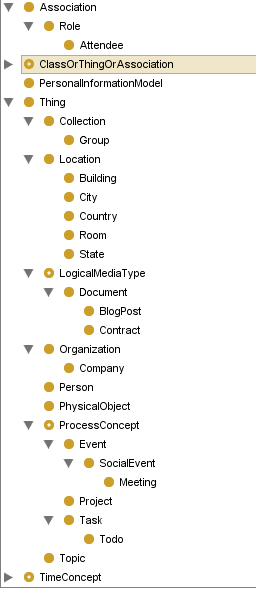
\includegraphics{images/upperclasses.png}
		\caption{Classes in PIMO-Upper}
	\label{fig:upperclasses}
\end{figure}

\begin{description}
%
%    NOTE !!!!!!!!!!!!!!!!!!!!!!!!!!!!!!!
%    These are copied from the ontology, and if not, the
%    descriptions have to be the same in the ontology and here.
%
	\item[Thing] The root class of the upper ontology. Every entity that can be in the direct attention of the user is a Thing.
	\item[Collection] A collection of Things, independent of their class. The items in the collection share a common property. Several usability studies showed that collections are important for PIM. It is recommended to either use the \texttt{pimo:hasPart} or the \texttt{pimo:isTagFor} relation to connect a collection with the Thing it contains\footnote{A Risk Of Change: A clear recommendation to either property may follow in future versions}.
	\item[Group] A group of Persons. They are connected to each other by sharing a common attribute, for example they all belong to the same organization or have a common interest.
	\item [Location] A physical location. Sub-classes are modeled for the most common locations humans work in: Building, City, Country, Room, State. This selection is intended to be applicable cross-cultural and cross-domain. City is a prototype that can be further refined for villages, etc.
	\item [LogicalMediaType] MediaConcepts are logical media types (e.g., a book, a contract, a promotional video, a todo list).  The user can create new logical media types dependent on their domain: a salesman will need MarketingFlyer, Offer, Invoice while a student might create Report, Thesis and Homework.
	\item [Organization] An administrative and functional structure (such as a business or a political party).
	\item [Person] Represents a person. Either living, dead, real or imaginary. In this regards, similar to \texttt{foaf:Person}.
	%\item [PhysicalObject] An object of interest in the physical world. \note{\emph{Knud}: if there is a physical object, how about an abstract object? Love? Language?
%\emph{Leo}: correct. I see a problem with Organozations and Topics, they have
%an overlap with AbstractObject. This can lead to a longer discussion...
%	we should consult sumo. I added this as an open issue at the end.\ref{issue:abstractobject}}	
%	It can be touched, it is concrete and it is of interest to the user. Examples are cars, tables, products and goods of business interest.
	\item[ProcessConcept] Concepts that relate to a series of actions or operations conducing to an end. Sub-classes are defined for Event, SocialEvent, Meeting, Project, and Task.
	\item[Topic] A topic is the subject of a discussion or document. Topics are distinguished from Things in their taxonomic nature, examples are scientific areas.
	\item[Tag] Tag is an abstract marker class to specify which Things in the user's PIMO should be considered useful tags in a tagging system. All Topics are Tags (Topic is a subclass of Tag). Implementations should support the user by using a useful set of Things as Tags, see Section~\ref{sec:tagginginpimo}.
\end{description}

These classes are intentionally kept generic. More specialized ontologies should be used for certain domains of application, see Section~\ref{sec:integratingontologies}. The classes of these ontologies are then  sub-classes of upper ontology classes. 

\subsection{Describing Things with Attributes and Relations}
\label{sec:describingthings}
Conventional RDF statements are used to describe Things. Predicates have to be defined as \texttt{rdfs:Properties} according to the NRL standard. Alternatively, it is also possible to use properties from other modeling languages like OWL or RDFS although we do not encourage this without a proper mapping of existing ontologies to PIMO (see~\ref{sec:integratingontologies}).

Properties that are intended to be editable and visible to end users \textbf{must} be sub-properties of either \texttt{pimo:datatypeProperty} or \texttt{pimo:objectProperty}.

Many NIE and NAO properties can be used from PIMO Things, see Section~\ref{sec:usingnieinpimo}. 

\subsection{Generic Properties in PIMO-Upper}
\label{sec:genericproperties}
The PIMO-upper ontology contains basic relations between Things and a few core attributes for identifying them (described above in Sect.~\ref{sec:identification}). 
These sub-properties of \texttt{pimo:objectProperty} are:
\begin{description}
  \item [\texttt{pimo:related}] is the most generic relation, giving no further indication how Things may be related. Related is defined to have itself as inverse property, 
  it is indirectly a \texttt{nrl:SymmetricProperty}, but does not inherit this attribute to sub-properties. Sub-properties can be asymmetric, depending on the inverse-of relation they define.
	\item [\texttt{pimo:hasPart}] and \texttt{pimo:partOf} model partitive relations. They are inverse. Neither is transitive, because part-of relations used for modelling in the domain of Personal Information Management are vague due to the many contexts of interpretation (a hotel may be part of a trip plan, a trip plan part of a project, but this does not indicate the hotel to be part of the project).
	\item [\texttt{pimo:hasTag}] and \texttt{pimo:isTagFor} connect a Thing of interest with a Tag characterizing it. For example, a meeting can have a project as a tag, or a document has a meeting as a tag, when the goal of the meeting is to discuss the document. After the meeting, the meeting minutes are a new Thing having the meeting as a tag. This is not restricted to meetings but also an organization or a person can have a certain technology as a tag to express that they are working on the topic described by the tag. The relation is not transitive, not symmetric. It is not asymmetric because a thing A may have thing B as tag, and B also A, if both are tags. The range of the \texttt{pimo:hasTag} relation is restricted to the class \texttt{pimo:Tag}. Topic is a subclass of tag. See Section~\ref{sec:tagginginpimo}.
\end{description}

Implementers may use these generic properties directly, or create sub-properties of them
or sub-properties of the more generic \texttt{pimo:objectProperty}.
The main reason to have the generic properties is the semantic meaning of the relations,
which can help to create user interfaces or model domains. 
Ontology authors can ask themselves ``does a new property model a part-of relation or not, does it assign a thing with a topic, or is it a generic relation?'' and then extend one of the generic properties.

For these generic relations, specialized sub-properties are defined when used on specific  classes in the PIMO upper ontology.

\subsection{Refined properties in PIMO-Upper}
\label{sec:pimoupperrelations}
Additional to the above relations, semantically interesting relations between PIMO upper classes are modeled. Especially those which can be used as symmetric or transitive relations for inference.

\begin{description}
	\item[\texttt{pimo:subTopic}] and \texttt{pimo:superTopic} relate Topics to each other. As Topics are an important mean to organize document collections based on a taxonomy, these two predicates are defined. They are inverse of each other and transitive.
	\item[\texttt{pimo:hasOrganizationMember}] and \texttt{pimo:isOrganizationMemberOf} are relations connecting a Person to an Organization.
	\item[\texttt{pimo:hasLocation}] and \texttt{pimo:isLocationOf} relate a locatable Thing with its Location. Locatable is an abstract sub-class of Thing.
	\item[\texttt{pimo:containsLocation}] and \texttt{pimo:locatedWithin} relate two locations within each other. Note that for geographic locations representing a physical space, inclusion is transitive.
\end{description}

\subsection{Tagging Things with Tags}
\label{sec:tagginginpimo}
% Say that PIMO is intended to work as an ontology, but also as a tagging system. When tagging e-mails or other elements, the name of the used tag must be unique. This is to be compatible with existing tagging systems, and to simplify the model. Intended use of TAG is to build a tag-cloud and organization system for the user's documents. Say that all topics are tags and are also arranged in a hierarchy (see next section). Recommend which classes make good tags: classes that exist for a longer time and can be used to classify many documents: topic, collection, group, city, person, organization, project. Say why it won't work without pimo:Tag. The classification system must be smaller than the document collection, to optimize retrieval.
The generic properties described in the last Sections show how Things can be related to each other.
An important aspect of PIMO is to classify Things using ``Tags''. 
Compared to normal PIMO Things, \emph{Tags} have one important additional restriction to make them compatible with Tags from other tagging system (folksonomies and Topic Maps):
\begin{itemize}
	\item The label of a Tag is unique, within the scope of one Personal Information Model.
\end{itemize}
Using Tags, PIMO can be used similar to an existing tagging system.

To extend a Thing to become a Tag, add the type \texttt{pimo:Tag}:
\begin{verbatim}
# The Person Dirk
claudia:DirkHagemann
  a pimo:Person;
# also a Tag
  a pimo:Tag;
# Must define the required pimo:tagLabel
  pimo:tagLabel "Dirk Hagemann".
\end{verbatim}
The \texttt{pimo:tagLabel} is required for all instances of \texttt{pimo:Tag}, and as it is a subproperty of \texttt{nao:prefLabel}, it can replace an existing prefLabel.
The \emph{intended use of Tags} is to build a clear category system for the user's documents. 
Once a Thing is \emph{tagged}, it can be retrieved by finding first the Tag, and then Things associated with the Tag.
A user's Tags are good candidates as first entry points to explore a data space, they can be visualized in a tag cloud or an alphabetical list. Tags can be clustered by type (each has an additional PIMO type), and by hierarchy (Tags can be organized in a part-of hierarchy, Topics are organized in a subTopic hierarchy).

To be useful as classification system, there should be a limited number of Tags to classify the potentially larger amount of documents. 
Examples are Things which exist for a longer period of time and Things that are of much importance to the user. 
Implementations \textbf{should} provide means to use the following as Tags.
\begin{itemize}
	\item All \textbf{Topics} can be considered Tags. This is expressed by the fact that Topic is a subclass of Tag.
	\item \textbf{Collections} work well as Tags, the act of putting something into a collection can be considered an act of tagging.
	\item A \textbf{person}.
	\item A \textbf{group of persons}. 
	\item A \textbf{city}, as there is a limited number of cities a person interacts with. 
	\item \textbf{Projects} are defined as an ``enterprise carefully planned'', the planning and execution of a project may involve tagging many Things as belonging to the project.
	\item A \textbf{task}, as documents may be needed to fulfill the task.
	\item An \textbf{organization} to classify to which organization a person belongs or by which organization a document was published.
\end{itemize}
The process of using an existing Thing as Tag \textbf{may} be automated. For example, a user searching for a possible Tag for a document should be able to pick from a list of existing Tags, and additionally search for Things of the above type to convert them to a Tag (such as a ``more Tags'' button). 
The conversion from Thing to Tag \textbf{may} then be automated and not visible to the user.

Tagging a document is illustrated in the following example, for more details refer to Section~\ref{sec:taggingfiles}.
\begin{verbatim}
claudia:BelfastMeetingPackage a claudia:MeetingPackage, pimo:Tag;
  pimo:tagLabel "Belfast Meeting Package".

claudia:BelfastBusTimetable a pimo:Document;
  pimo:groundingOccurrence <file://home/claudia/doc/tripplan.pdf>;
  pimo:hasTag claudia:BelfastMeetingPackage.
\end{verbatim}

In general, it should be avoided to use \texttt{pimo:Document} instances as Tags.
Typically the amount of documents is high, making them less useful as categorization scheme compared to the above mentioned Thing classes. 
The reason to introduce Tags in PIMO is to allow implementers to separate between categorization scheme and annotated instance base (which is usually a document corpus).
Without a class to mark Tags, it would not be possible to restrict the \texttt{pimo:tagLabel} predicate to a minimum cardinality of one, and also Topics could not automatically be defined as Tags.

\subsection{Topic Hierarchies}
\label{sec:topichierarchies}
% say that PIMO is a taxonomy system comparable to SKOS. The hierarchical ordering of Topics is important to organize the system. Hierarchies are also used to allow semantic search on subtopic structures. add rules.
The methodologies so far allow the description of individual Things with labels, properties, classes, and Tags. 
Besides the view on individuals, their place inside an overall organization scheme of the user can be important --- where is a Thing located in a hierarchy? 
Things can be placed in a hierarchy using the \texttt{pimo:hasPart} relation. 
In an overall hierarchy, the part relation can be confusing, as Things both have a class and can be part of something. For example, \emph{workpackage 2} is \emph{part of } the \emph{CID project}. In a combined hierarchy including class and part-of relations, it would appear at two positions: as instance of workpackage and as part of CID. 

To simplify the system for novice users, it is \textbf{recommended} for implementers to support a \emph{Topic Hierarchy}, where hierarchical part-of structures are shown to end-users. The semantic ``is-a'' relations \textbf{should} be hidden in the Topic hierarchy.
This allows users to model parts of their PIMO as taxonomy.
\begin{itemize}
	\item Each instance of \texttt{pimo:Topic} \textbf{must} either have a \texttt{pimo:hasSuperTopic} relation to another Topic or be defined as root Topic using \texttt{pimo:hasRootTopic}.
	\item All Topics \textbf{must} be connected (indirectly or directly) to a root Topic, or be a root Topic themselves.
	\item User interfaces \textbf{should} render Topics using the hierarchical structure.
	\item Cycles in the super-topic structure are allowed but \textbf{should} be avoided.
	\item A Topic can have multiple super Topics, PIMO allows poly-hierarchical structures.
	\item The \texttt{pimo:subTopic} and \texttt{pimo:superTopic} relations are defined \emph{transitive}. 
	\item When displaying Topics in hierarchical user interfaces, the transitivity of \texttt{pimo:subTopic} \textbf{should} not be inferred. The user experience should be the same when modelling and when browsing the hierarchy.
	\item When searching for Things using the \texttt{pimo:hasTag} relation, the transitivity of \texttt{pimo:subTopic} \textbf{should} be inferred, see below.
\end{itemize}

To support \emph{semantic search} in Topic hierarchies, the following rule for tagging does apply when searching for Things using the hasTag relation (for a detailled description, see Section~\ref{sec:pimorules}):
\begin{verbatim}
CONSTRUCT 
{?x pimo:hasTag ?B.} 
WHERE 
{?x pimo:hasTag ?A. 
?A pimo:superTopic ?B.}
\end{verbatim}

The hierarchical structure of Topics in PIMO is comparable to the modeling in SKOS\cite{SkosStandard}. The \texttt{pimo:subTopic} relation is equivalent to \texttt{skos:narrowerTransitive}.
PIMO requires all Topics to be connected to root Topics, SKOS does not require this in the semantics of \texttt{skos:hasTopConcept}.

\subsection{Creating Personalized Classes and Properties}
\label{sec:customontology}
The predefined classes and properties are intended as a generic basis to be extended.
The user can always create new classes and property types, or existing ontologies can be imported (see Section~\ref{sec:pimomid}).
A number of requirements apply:
\begin{itemize}
	\item The superclass has to be \texttt{pimo:Thing} or a sub-class.
%	\item The property pimo:isDefinedBy has to be set to express that the user created the % class.
	\item The class has to be labelled with \texttt{nao:prefLabel}.
	\item The class has to be related to the user's PIMO with \texttt{pimo:isDefinedBy}.
\end{itemize}

Similarly for custom properties:
\begin{itemize}
	\item The property has to be labelled with \texttt{nao:prefLabel}.
	\item The property has to be related to the user's PIMO with \texttt{pimo:isDefinedBy}.
\end{itemize}
For properties that relate two things, the following applies:
\begin{itemize}
  \item The property \textbf{must} be a sub-property of \texttt{pimo:objectProperty} (either directly or indirectly via inference).
	\item The super-property \textbf{should} be one of \texttt{pimo:related}, \texttt{pimo:hasTag}, \texttt{pimo:isTagFor}, \texttt{pimo:hasPart}, or \texttt{pimo:partOf}.
	\item An inverse property \textbf{must} be defined. Inverse properties define the semantic meaning in both ways, which is required for 
user interfaces showing relations.
\end{itemize}
For custom properties that have \emph{a literal or datatype as range} the following applies:
\begin{itemize}
  \item They must be a sub-property of \texttt{pimo:datatypeProperty}.
  \item Inverse properties should not be defined (as Literals cannot be subject of statements, inverse does not apply anyway).
\end{itemize}

For all custom-created properties and classes, 
modification dates \textbf{must} be set.

\subsection{Collections of Things}
\label{sec:collections}
In Personal Information Management, grouping multiple Things into one collection is a crucial feature. Today's hierarchical file systems are a good example: a folder can be created to contain multiple elements. Later, actions on this folder, such as compressing it, or deleting it are supported.
The generic \emph{has Part} relation provides the semantics of putting a Thing into another Thing. For usability reasons, we also provide a class \texttt{pimo:Collection} to be used for generic collections of multiple items.

Applications that want to present the complex possibilities of PIMO in a simpler way can offer collections. 
First, an instance of the class \texttt{pimo:Collection} is created. Then, elements are added to the collection using the \texttt{pimo:hasPart} relation. 
A typical application of collections is the list of ``Favourites'' containing recently used and important resources.

Collections are unordered, the ordering of items inside the collection can be done using alphabetical order, time, geographic location (if they are locatable), or type.

Tags are another simplification, described below in Section~\ref{sec:taggingfiles}.

%\begin{itemize}
%	\item collections are unordered
%	\item temporal order is expressed using implizit modeling (the time difference is implicit and has to be calculated for explizit knowing it for sorting)
%	\item in science, different sorting systems are described: geographical, alphabetically,  by Time, by Categories, by Hierarchy.  (Location, Alphabet, Time, Category, and Hierarchy, known as LATCH  cite R. Wurman, D. Sume, and L. Leifer, Information Anxiety 2, Que, 2000.)
%	\item Latif and Tjoa, 2006 \cite{Latif+2006} have existing systems are build on LATCH, and additionally refine it saying that hierarchy is often taxonomic and that people are an important ordering factor, as also does Dengel2006.
%	\item That said, we see that ordering is dependent on the view in the application and on the attributes of the elements, there is a reason WHY the elements are ordered in a way based on their attributes. For PIMO, we do not provide an explicit sort order (before/after) relations, this can be added by implementers as extensions. The NEPOMUK Conceptual Elements model, developed by Max V�lkel and Heiko Haller defines the standards for ordering. On the level of PIMO, ordering of items in a collection is implizit by the attributes of the items in the collection and handled by the user interface, by showing the elements in whatever order is appropriate.
%	\item The Collection class can be used to model collections of items that share a common attribute. 
%	\item Members of collection are modeled using hasPart.
%\end{itemize}

\subsection{Modeling Associations and Roles in PIMO}
\label{sec:roleBasedModeling}
Often there is a need to add meta-data about a relation, for example the date of creation of a relation. 
In RDF, this is typically done using reification, and then adding meta-data about the 
reified Statement using an instance of the class \texttt{rdf:Statement}. 
A problem with reification is that when using the generic class \texttt{rdf:Statement}
to represent it, there are no guidelines which properties are now suitable to annotate the statement.
More precise sub-classes of Statement would solve this.
Another problem is that \emph{n-ary} relations cannot be expressed with triple statements.

In PIMO, \textbf{Associations} are used to add metadata about relations and to create
n-ary relations. They are entities representing the relation of multiple Things with each other.
Each Thing part of an Association is related to the association using the \texttt{pimo:associationMember} property or more precise sub-properties of it.

As an example, the fact that Claudia attended a meeting can be expressed using the \texttt{pimo:Attendee} role.

\begin{verbatim}
claudia:AttendsInitialMeetinginBelfast a pimo:Attendee;
  pimo:attendingMeeting claudia:InitialMeetinginBelfast;
  pimo:roleHolder claudia:Claudia.
\end{verbatim}

Here, the class \texttt{pimo:Attendee} is a sub-class of \texttt{pimo:Association}
and represents the association as such (``this is an association between a person and a meeting''). The two relations used are sub-properties of \texttt{pimo:associationMember} and identify the two Things to relate, the specific relations determine the role taken by each Thing. 
New sub-classes of association can be created when needed, also new sub-properties
of \texttt{pimo:associationMember} for more specific roles. 

Associations are elements of a user's PIMO and \textbf{must} be connected to the user's PIMO with a \texttt{pimo:isDefinedBy} relation.
Modification dates are to be handled the same way as with Things (see Section \ref{sec:changedates}).

\section{Connecting PIMO to Information Elements}
\label{sec:pimoVSnie}
In the last section, the Things created within a user-PIMO were described.
They are to be unique, described with defined ontologies,
and ought to be identified well.
The next step is to connect these to the files, e-mails, and other Information Elements
which exist in the user's PSI.
These are ambiguous, described in various ontologies, and in general more chaotic when compared to the user-PIMO.
The crucial point is to use Things as organization scheme to classify and integrate
existing data found in a PSI.

The first step is to \textbf{connect Things to Information Elements} that represent them.
As described above (Section \ref{sec:identification}), the \texttt{pimo:groundingOccurrence}
and \texttt{pimo:occurrence} relations are to be used to connect them.
This connection has the semantics of a unification --- both the Thing and the Information Element represent the same real-world entity. 
But the Thing is the unique, static representation that should be used to annotate the entity.
Implementations \textbf{should not} allow the users to annotate Information Elements directly, instead it is \textbf{recommended} to connect the Information Element to a Thing using \texttt{pimo:groundingOccurrence} and then annotate the Thing.
The rationale is that Information Elements can change their URI, be deleted or moved, and then the annotations may be disconnected from the described resource. 

Creating a Thing for each annotated document will result in vast amounts of instances in the sub-classes of \texttt{pimo:Document}, as users can likely have access to thousands (sometimes millions) of documents. To navigate effectively through such large structures, PIMO Topics can be used to annotate documents using the \texttt{pimo:hasTag} relation.

How to annotate documents using PIMO is described in Section \ref{sec:taggingfiles}.

\subsection{Connecting Things and Classes to Folders}
\label{sec:containers}
Things can also be connected to folders in the file-system to express that
these folders contain information related to the thing. 
Use the \texttt{pimo:hasFolder} relation to connect a Thing or a Class with a folder.
The semantic meaning of this relation is not formally restricted but open to be used in various ways.
For folders connected to Things, it is \textbf{recommended} 
to interpret the content of the folder as ``having the Thing as topic''.
Implementers \textbf{may} add a \texttt{pimo:hasTag} relation between the Things inside the folder and the Thing. 

For folders connected to Classes, it is \textbf{recommended}
to interpret the content of the folder as ``being an instance of the Class''.
Implementers \textbf{may} add a \texttt{rdf:type} relation between the Things inside the folder and the Class.

In all cases, files or other information elements in folders have to 
be represented as Things first, before further annotation (see Section \ref{sec:creatingthingalgorithm}).

The property \texttt{pimo:hasFolder} \emph{can} be used by implementers
to suggest folders for information elements --- if an information element
is annotated with a \texttt{pimo:hasTag} relation to a topic that is connected
to a folder, this is an indication to move the element to the folder, if needed.

\subsection{Integrating Facts about Things}
\label{sec:integratingfacts}
The unification of multiple Information Elements into one Thing is also 
on the level of facts, RDF statements.
To answer the question ``when did I last communicate with people shown on this
picture'' can only be answered when facts from multiple sources (e-mails, photos, photo annotations and the user-PIMO) can be queried as one model.
The statements about the Information Elements connected to a Thing via \texttt{pimo:groundingOccurrence} and \texttt{pimo:occurrence} can be \textbf{superimposed} to the Thing.
The exact rules are given in Section \ref{sec:creationrules} and directions
how to use them are in Section \ref{sec:unification}.

Through this process, a view on the data is generated.
The user can get an overview of all existing data --- in an integrated way --- and then
drill down into specific occurrences.
In this view, it is possible that a Thing has multiple classes (as \texttt{rdf:type}),
one from the level of PIMO ontologies and others from the integrated Information Elements.
In the example given in Section \ref{sec:unification}, 
Dirk Hagemann is inferred to be both a \texttt{pimo:Person}
and a \texttt{pimo:PersonContact}. 
The two classes are not required to be sub-classes of each other.
To get a coherent and meaningful view, the class of the InformationElement (or related resource) \textbf{may} be related to a PIMO class using the \emph{pimo:hasOtherConceptualization} relation, as described later in Section~\ref{sec:integratingontologies}.

It is not required that the used ontologies are formally aligned and mapped.
Rather, it is assumed that the user will be able to interpret the statements based on his knowledge about the data in his PSI.

The details about the integration of facts are given in Section \ref{sec:unification} on \emph{unification}.
 
\section{PIMO-group level: Group and Domain ontologies}
\label{sec:pimomid}
% In this section we introduce the idea of specializations of 
% PIMO upper that are shared amongst companies and groups.
% COPIED FROM SauermannElstDengel2007
The upper (foundational) level of \pimo just makes a few, basic
ontological statements about Things which exist on a Semantic Desktop, \ie Things which
are essential in a knowledge worker's mental model.
In order to avoid a \emph{cold start problem}
\footnote{The problem of cold starts is well known in knowledge-based systems: In the beginning a system, such as a shell, has little or no information and therefore doesn't seem to be useful to a new user. 
Consequently, they are not motivated to invest in using and feeding the system with new
information, which again would be a prerequisite for it to be \emph{more} useful. Enter vicious cycle...} 
with PIMO-based
applications, more ontologies defining concepts shared within groups 
or modeling domains are needed.
The user's company and its organizational structure may be such a domain, or a shared public ontology.
Classes are refinements of PIMO-Upper, allowing an integration
of various domain ontologies via the upper layer.

In the following section, recommendations are given how to model group and
domain level ontologies.

%\section{Mapping ontologies to PIMO-upper}
\section{Extending PIMO}
\label{sec:integratingontologies}
%\note{Knud: I changed the title, because I think this chapter is not only about mapping ontologies, but more generally speaking about how to extend PIMO for one's needs. Leo: perfect.}
%\note{Leo: this section should be either merged with the previous one, or the previous one removed. Both is fine, removing above is probably nicer.}
Out of the box, PIMO is kept sufficiently simple and only contains relatively few classes and properties. This was done in order to ensure that the ontology is general enough to apply to almost any relevant domain. 
% removed. see https://dev.nepomuk.semanticdesktop.org/ticket/534
%At the same time, PIMO contains enough basic elements to allow the user to start working straight away and prevent the cold start phenomenon. 
However, as soon as the set of pre-existing classes and properties becomes too narrow and confining, it is a very simple matter to extend PIMO and add domain-specific extensions, or map external ontologies onto PIMO. E.g., PIMO can easily be extended to express the organizational structure of the user's workplace, a biological classification system, or to include a PIMO-version of the BibTeX vocabulary.
These \emph{domain ontologies} differ from \emph{personalized classes and properties} (see Section \ref{sec:customontology}) by the fact that they are not created by the user,
but created by a third party for multiple users.
\subsection{Refining Elements of PIMO-upper} % (fold)
\label{sub:subclassing_pimo_upper}
Creating group--level ontologies is a simple matter of \textbf{defining new sub-classes of PIMO-upper classes (see Sect.~\ref{sec:pimoUpperClasses}) or sub-classing \texttt{InformationElement} classes}. 
If needed, new properties can also be added, which apply to the new classes via domain or range.
Importing created \emph{group--level ontologies} into a user's PIMO is described in the next Section (\ref{sec:importingontologies}).

\paragraph{Classes} % (fold)
\label{par:classes}
 
%\note{Leo 13.12.: The individual values for Grades are a good example where instances must be added to domain ontologies. Could you add the grades such as teaching:GradeA, teaching:GradeB, teaching:GradeC, ... teaching: GradeF and give them preflables ``A''..''F'' ? This also looks good in N3. The argumentation is that teachers can then search for Students having grade ``A''.. etc ... and these are shared amongst teachers.}
%\note{Knud, 05.01: Done! :)}
%\note{Leo 13.12: in general, instances can be added to domain ontologies when they are shared amongst all users, for example a school may publish a domain ontology with instances for all teachers and personnel, and typical courses for each year to take the burden of modeling away from the teachers}
% Leo: commented out above notes, they are DONE!
As an example, you may work in the domain of teaching and training, and therefore want to extend PIMO with elements specific for this domain, such as \emph{courses}, \emph{lessons}, \emph{teachers} or \emph{students}. In this case, you would look for existing PIMO-upper classes which could be considered generalizations of your new classes. E.g., a course would be a sub-class of \texttt{pimo:ProcessConcept}, training lessons could be a sub-class of \texttt{pimo:Meeting}, teachers and students could be sub-classes of \texttt{pimo:Person} (or \texttt{pimo:Role} --- role-based modeling is discussed in Sect.~\ref{sec:roleBasedModeling}) and training material a sub-class of \texttt{pimo:Document}. Since all pre-existing PIMO-upper classes derive from \texttt{pimo:Thing}, all your new classes automatically do as well (except for roles: \texttt{pimo:Role} is not a sub-class of \texttt{pimo:Thing}). 

There could also be cases where no existing PIMO-upper class seems to apply to your new class --- in this case, the new class would directly derive from \texttt{pimo:Thing}. Consider, e.g., that you want to include the concept of \emph{grades} in your PIMO. There isn't really a good pre-existing superclass for grades in PIMO-upper, so your new \texttt{Grade} class would be a direct sub-class of \texttt{pimo:Thing}.

Even if there might be a potential superclass, it may be wise to postpone this decision if one isn't completely sure, and instead just sub-class \texttt{pimo:Thing}. It is always easier to add a superclass relationship later, rather than make a bad decision now and then have to deal with incorrect data at a later stage.

If needed, the new classes can also have sub-class relationships into other ontologies, such as other NIE-based ontologies or completely different ontologies such as WordNet\footnote{\url{http://wordnet.princeton.edu/}}, SUMO\footnote{\url{http://www.ontologyportal.org/}}, or Dolce\footnote{\url{http://www.loa-cnr.it/DOLCE.html}}.

% paragraph classes (end)

\paragraph{Instances} % (fold)
\label{par:instances}

In some cases, you will also want to add instances of classes to the ontology you are integrating with PIMO. This makes sense if those instances are shared and used among a many users. An example are actual grades that a teacher might gives their students, such as grades from A--F. Each such grade (\texttt{teaching:GradeA}, \texttt{teaching:GradeB}, etc.) is an instance of the class \texttt{Grade}, but since those instances will be used by all teachers and students, they can become part of the teaching ontology. Similarly, if a school decides to introduce the teaching ontology, they might include instances for all their teachers, students, classes, courses, etc.

% paragraph instances (end)

\paragraph{Properties} % (fold)
\label{par:properties}

New properties can then refer to the new classes via domain or range and thus further specify them. Examples are the relation between courses and teachers/instructors (e.g., \texttt{teachesCourse(Teacher, Course)}) or between course material and a course (e.g. \texttt{courseMaterialFor(CourseMaterial, Course)}). This example is illustrated graphically in Fig.~\ref{fig:extensionExampleTeaching}, as well in N3 source code in Fig.~\ref{fig:extensionExampleTeachingN3}. This approach is a \textbf{typical example of how to integrate domain ontologies for specific application areas into PIMO}.

There are some general guidelines for introducing new properties:
\begin{itemize}
	\item Properties which connect two \texttt{pimo:Thing}s (or sub-classes) should be defined as sub-properties of \texttt{pimo:related}, \texttt{pimo:hasTag}, \texttt{pimo:isTagFor}, \texttt{pimo:hasPart}, or \texttt{pimo:partOf} (see Sect.~\ref{sec:genericproperties}). By relating new, specialized properties to the more generic PIMO properties, the new ontology can integrate better with existing desktop environment. When not extending the generic properties, at least new properties should exted \texttt{pimo:objectProperty}.
	\item All new object-properties \textbf{must} define an inverse property, as required
	in Section~\ref{sec:customontology}.
	\item Identifying properties (such as a name) that have domain \texttt{pimo:Thing} and a literal range should be mapped as sub-properties of \texttt{nao:identifier}. An example is give in Fig.~\ref{fig:bibtexExample}.
	\item 
% Leo 8/1: removed the note, the fix seems to be accepted by Knud.
%\note{\emph{Knud}: I don't understand this at all. Leo: I splitted it up to two items and explained the concept of referencing occurrences a little.}
	Some new properties may be defined as sub-properties of \texttt{pimo:referencingOccurrence} (see Sect.~\ref{par:referencingOccurrence}). This is true for all object properties (i.e., properties which have a resource range and not a literal range) which describe or identify the subject in an unambiguous way. In other words, the object resource   exclusively describes the subject. A typical example is \texttt{foaf:homepage}: two different people would most likely not have the same homepage (ignoring exceptions such as family homepages). If, however, we come across two different RDF resources which have the same \texttt{foaf:homepage}, we can assume that they describe the same real-life person.
	  \item A frequent situation in Semantic Web and Semantic Desktop scenarios is that the same real-life object (i.e., a person, country, project, etc.) is defined as a resource in many different ontologies. The PIMO property \texttt{pimo:hasOtherRepresentation} is used in such cases. If your new ontology contains a property which expresses a similar (more specific) relation between resources, then it should be a sub-property of \texttt{pimo:hasOtherRepresentation} (see Sect.~\ref{par:otherRepresentation}). In the vanilla SW world, a similar property is \texttt{rdfs:seeAlso}.
\end{itemize}

% paragraph properties (end)

\begin{figure}
  \begin{center}
    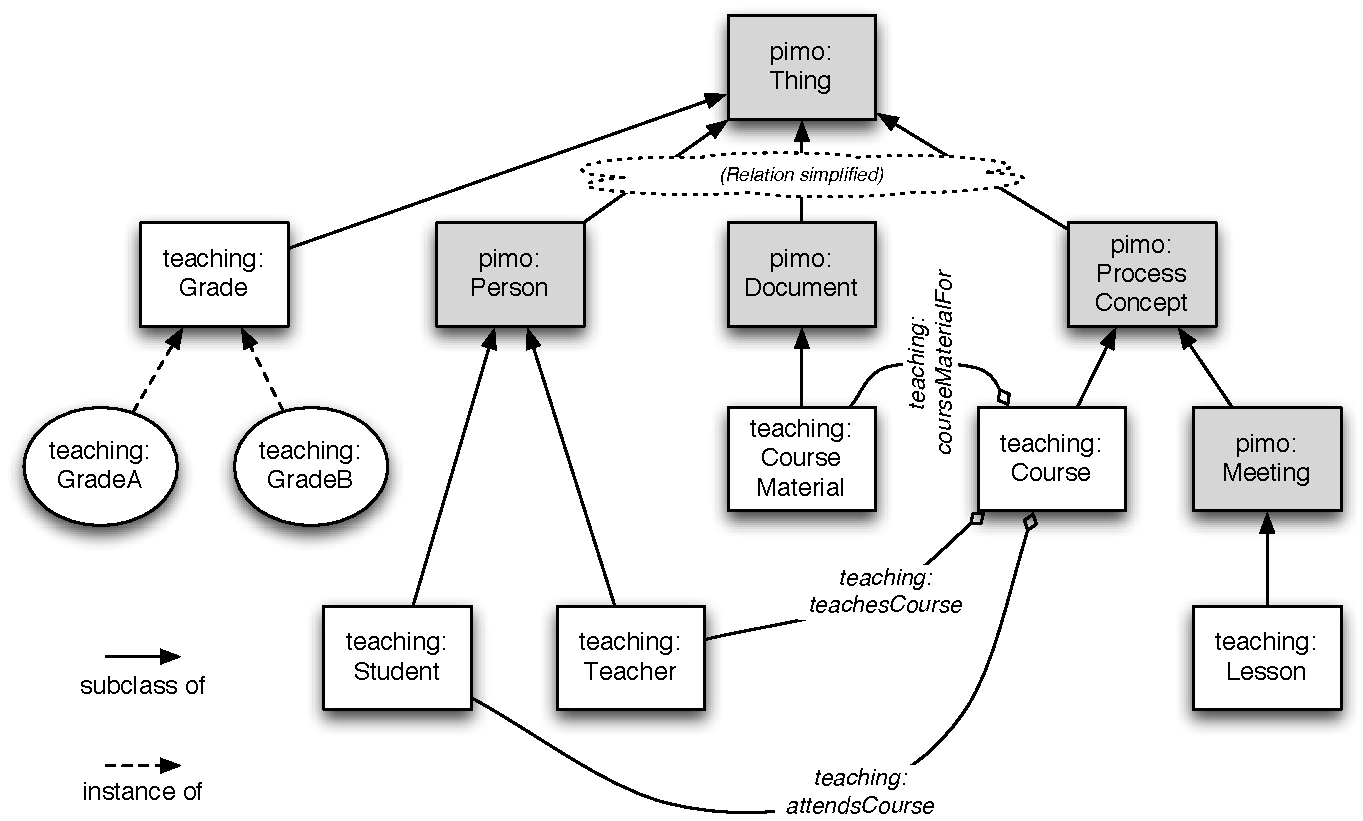
\includegraphics[width=\linewidth]{images/PIMOextensionExample-Teaching}
    \caption{Extending PIMO with new classes, properties and instances for the domain of teaching}
    \label{fig:extensionExampleTeaching}
  \end{center}
\end{figure}

\begin{figure}
  \begin{center}
	\begin{verbatim}
# new classes:
   teaching:Grade a rdfs:Class;
      rdfs:subClassOf pimo:Thing.

   teaching:Student a rdfs:Class;
      rdfs:subClassOf pimo:Person.

   teaching:Teacher a rdfs:Class;
      rdfs:subClassOf pimo:Person.

   teaching:CourseMaterial a rdfs:Class;
      rdfs:subClassOf pimo:Document.

   teaching:Course a rdfs:Class;
      rdfs:subClassOf pimo:ProcessConcept.

   teaching:Lesson a rdfs:Class;
      rdfs:subClassOf pimo:Meeting.

# new properties and their inverse:
   teaching:courseMaterialFor a rdf:Property;
      rdfs:subPropertyOf pimo:partOf;
      rdfs:domain teaching:CourseMaterial;
      rdfs:range teaching:Course;
      nrl:inverseProperty teaching:hasCourseMaterial.
   teaching:hasCourseMaterial;
      rdfs:subPropertyOf pimo:hasPart;
      rdfs:domain teaching:Course;
      rdfs:range teaching:CourseMaterial;
      nrl:inverseProperty teaching:courseMaterialFor.

   teaching:teachesCourse a rdf:Property;
      rdfs:subPropertyOf pimo:related;
      rdfs:domain teaching:Teacher;
      rdfs:range teaching:Course;
      nrl:inverseProperty teaching:taughtBy.
   teaching:taughtBy a rdf:Property;
      rdfs:subPropertyOf pimo:related;
      rdfs:domain teaching:Course;
      rdfs:range teaching:Teacher;
      nrl:inverseProperty teaching:teachesCourse.
      
   teaching:attendsCourse a rdf:Property;
      rdfs:subPropertyOf pimo:related;
      rdfs:domain teaching:Student;
      rdfs:range teaching:Course;
      nrl:inverseProperty teaching:attendeeStudent.
   teaching:attendeeStudent a rdf:Property;
      rdfs:subPropertyOf pimo:related;
      rdfs:domain teaching:Course;
      rdfs:range teaching:Student;
      nrl:inverseProperty teaching:attendsCourse.

# new instances:
    teaching:GradeA a teaching:Grade;
      nao:prefLabel "A".

    teaching:GradeB a teaching:Grade;
      nao:prefLabel "B".

    ...
	\end{verbatim}
    \caption{Extending PIMO with new classes, properties and instances for the domain of teaching --- N3 code}
	\label{fig:extensionExampleTeachingN3}
\end{center}
\end{figure}

\paragraph{Inheritance} % (fold)
\label{par:inheritance}

Sub-classing any class from PIMO (whether it be existing classes from PIMO-upper or classes that have been added later) also means that the new sub-class can be used with the same properties that have been defined with its superclass. Remember that NRL has a closed world assumption, and not an open world assumption, as RDFS traditionally has. In NRL\footnote{\url{http://www.semanticdesktop.org/ontologies/nrl/}}, ontologies can be used to validate statements.
%\note{reference to NRL spec --- 05.01.08, done}
E.g., if the property \texttt{name(pimo:Person, String)} has been defined, and if we define our new class \texttt{teaching:Student} to be a sub-class of \texttt{pimo:Person}, then this will allow us to use \texttt{name} with instances of \texttt{Student} as well - an NRL validator will permit this, because all instances of \texttt{Student} are also instances of \texttt{Person}. An example of this is shown in Fig.~\ref{fig:propertyInheritance}: this concept is very similar to the idea of inheritance in object-orientation, even though strictly speaking it is not the same.

% paragraph inheritance (end)

\begin{figure}
  \begin{center}
	\begin{verbatim}
		
   pimo:name a rdf:Property;
      rdfs:Domain pimo:Person;
      rdfs:Domain rdfs:Literal.
		
   teaching:Student a rdfs:Class;
      rdfs:subClassOf pimo:Person.

   knud a teaching:Student;
      pimo:name "Knud M�ller".

	\end{verbatim}
    \caption{``Inheritance'' of properties}
	\label{fig:propertyInheritance}
\end{center}
\end{figure}

% subsection subclassing_pimo_upper (end)

\subsection{Markup for the new ontology}
\label{sec:extendingontologymarkup}
The teaching ontology still needs to be defined as proper NRL ontology
to be usable with PIMO. The ontology \textbf{must} to be identified via its URI
and the author of the ontology can be added
as \texttt{nao:creator}.

\begin{verbatim}
teaching:TeachingOntology a nrl:Ontology;
 nao:creator teaching:TeachingOntologyCreator.

teaching:TeachingOntologyCreator a nao:Party;
 rdfs:label "Knud M�ller".

\end{verbatim}

\subsection{Information Elements} % (fold)
\label{sub:information_elements}

An important feature of the NEPOMUK ontology architecture is the fact that it is divided into two tiers: the PIMO tier and the Native Structures tier, as defined in the NEPOMUK Information Element Ontology (NIE)\footnote{\url{http://www.semanticdesktop.org/ontologies/nie/}} and its sub-ontologies, such as the NEPOMUK File Ontology (NFO)\footnote{\url{http://www.semanticdesktop.org/ontologies/nfo/}}.
%\note{reference to NIE spec --- 05.01.08, done}
While the former covers the internal mental model of a user or an organization (people, events, projects, etc.), the latter covers the physical representations of data (address book entries, calendar entries, files, etc.). Obviously, there are numerous connections between the tiers: people are represented by address book entries, events appear in the calendar, projects have files associated to them.

Whenever classes that are introduced to PIMO have a physical representation on the user's desktop, a connection to NIE must be modeled as well. Consider the example of the teaching ontology above: Such an ontology will contain classes for Things like exams and essays. Those classes belong to the PIMO tier. Their representation within the computer --- e.g., as text files --- belongs to the native structures tier. Or, in a more complex case, the new ontology could very well come with a specialized application, such as a Training Course Manager, where users can assign attendees to trainings, etc. In this case, people and courses (PIMO tier) would be represented by the application as application-specific data structures or information elements (native structures tier). In both cases a link from the new PIMO classes to the information elements represented with NIE is required to fully exploit the possibilities of the semantic desktop.

% subsection information_elements (end)

%\note{Knud, 05.01.08: I decided to drop the Author class in the BibTeX example. Authors should really just be pimo:Persons, not a subclass thereof.
%Leo, 8/1: OK, DONE}

As a second example, we can consider an ontology for scientific publications. This ontology (which would probably be based on Bib\TeX), would come with classes such as \texttt{Article} or \texttt{Book} and relations between them like \texttt{bookContainsArticle} or \texttt{hasAuthor}. For the integration into PIMO, \texttt{Article} would most likely become a sub-class of \texttt{pimo:Document}. 
Documents have	two types: one which anchors them in the PIMO tier, and one which anchors them in the native structures tier.
The \texttt{pimo:LogicalMediaType} (and its sub-classes, e.g., \texttt{pimo:Document}) captures how a document is interpreted by the user and belongs to the PIMO tier. Logical media types can be contracts, invoices, assignments, invitations, law texts, etc. 
The other type, which is the \texttt{nfo:Document} type, captures how the system interprets the document, and belongs to the native structures tier.
This is the physical document type as modeled by NIE.
Instances of a logical media type can have various representations in the native structures tier: 
for example, a text interpreted as an invoice by the user can either be an \texttt{nfo:PlainTextDocument} or an \texttt{nfo:PaginatedTextDocument}. 
Vice-versa, one physical type can be used to represent both an invitation or an invoice, which are different logical media types.
Keeping this this separation of content and representation in mind, one can model concrete documents having two types, one on each tier.

\begin{figure}
  \begin{center}
\begin{verbatim}
bibtex:Article a rdfs:Class;
 # PIMO tier: interpreted by the user as nie:Document
 rdfs:subClassOf pimo:Document; 
 # native structures tier: interpreted by the system as nfo:TextDocument
 rdfs:subClassOf nfo:TextDocument. 

bibtex:hasAuthor a rdf:Property;
 rdfs:subPropertyOf pimo:related;
 rdfs:subPropertyOf nfo:creator;
 rdfs:domain bibtex:Article;
 rdfs:range pimo:Person.
 
bibtex:hasLCCN a rdf:Property;
 rdfs:subPropertyOf nao:identifier; \# add an identifier
 rdfs:domain bibtex:Article.
\end{verbatim}
    \caption{A Bib\TeX-based PIMO extension for scientific publications}
	\label{fig:bibtexExample}
\end{center}
\end{figure}
%bibtex:Author a rdfs:Class; 
% # this adds properties like Name
% rdfs:subClassOf pimo:Person. 

\subsection{Extension by Sub-classing from External Classes} % (fold)
\label{sub:extension_by_subclassing_from_external_classes}

\textbf{Another possibility is extending existing PIMO-upper classes by sub-classing them from external classes.} \emph{This is discouraged}. For example, if the class \texttt{pimo:Person} was defined a sub-class of \texttt{nco:PersonContact} and \texttt{pimo:Organization} a sub-class of \texttt{nco:OrganizationContact}, all instances of these classes would automatically be inferred to be \texttt{pimo:Thing}s. However, those instances would probably not have some of the properties required by the \texttt{Thing} defined, which would render the imported data invalid. 
Similarly, when a mapped class X has cardinality restrictions on its properties (such as required properties), adding X as new superclass to an existing PIMO class can render the instances of the PIMO class invalid. 

% subsection extension_by_subclassing_from_external_classes (end)

\subsection{Summary} % (fold)
\label{sub:summary}

The very condensed summary to extending PIMO and mapping frome existing ontologies to PIMO is the following:

\begin{itemize}
  \item Make classes sub-classes of PIMO-upper classes.
  \item Make properties sub-properties of PIMO-upper properties.
	\item Relations: Links between Things have to be browseable, properties should have inverse relations defined (see \cite{rohmer2005})
	\item Extensibility: Users are free to add new relation types and new classes (see \cite{rohmer2005})
\end{itemize}

% subsection summary (end)

\section{Importing Domain Ontologies into a User's PIMO}
\label{sec:importingontologies}
%\note{Written by Leo, but Knud: feel free to mash it up}
Once modeled, the new domain ontology such as the teaching ontology in the previous examples can be made available publicly for others, for example by publishing it on the Web. A good reference for doing this is \emph{Best Practice Recipes for Publishing RDF Vocabularies}~\cite{SWBPVocabularyRecipes}.

% adressing
Semantically, an imported ontology is captured using a \texttt{nrl:imports} statement.
When a user imports a domain ontology, this statement \textbf{should} be added.

{\small
\begin{verbatim}
claudia:Pimo nrl:imports teaching:TeachingOntology.
\end{verbatim}
}

%Importing the ontology to a Sematic Desktop or other Personal Information Management system can then be done by downloading the ontology file and storing it into the RDF store where the PIMO of the user is kept.
% Stuff like downloading is outside the scope of PIMO and really has no place in the PIMO specification
Once the user of a Semantic Desktop system imports an external PIMO into their own desktop, all new classes (which are sub-classes of \texttt{pimo:Thing}) \textbf{should} become available to them as if they had created those classes themselves.
Instances, on the other hand, are not automatically available.
As said in the introduction, the scope of a PIMO for an individual user is to model data that is within their own attention and needed for knowledge work or private use.
However, when importing external ontologies or knowledge bases, not all instances may be of interest to the user. As with imported information elements, a separate Thing is created to represent the imported resource within the PIMO of the user and connected to the imported instance using \texttt{pimo:hasOtherRepresentation}\footnote{An alternative would be to treat all Things present in the RDF data available of the user as if they were created by the user, imported or not. This has the drawback that it allows to represent the same real-world entity twice, first in the imported domain ontology and second in the user's own PIMO.}.
Before creating a new Thing for an imported instance, the PIMO of the user has to be checked if the entity is already represented as a Thing, as indicated above in Section~\ref{sec:creatingthingalgorithm}.
Once represented as a Thing in the user's PIMO, it is possible to assign a personal identifier to it, annotate it, and use it. 

Implementations \textbf{must} automate the importing process. The user should be able to interact with imported Things as if they were created by themselves. 

\begin{comment}
LEO: THIS COMMENTED OUT NOW, ITS TOO SCIENTIFIC.
\section{Design Rationale}
\label{sec:designrationale}
In this section the design rationale behind \pimo and the sources which influenced us are described. 
% COPIED FROM SauermannElstDengel2007
%The motivation for creating the PIMO is to find a language to name the terms
%that are relevant to a knowledge worker and to have ways to express facts about
%these terms. Once this language is defined and formalized in the ontological
%description of the PIMO, it can be used to translate existing resources, and to
%express information about them. The PIMO is a user-centric view on existing
%documents, domain ontologies, and web data sources.
%
%While the organization asks for universally applicable and standardized
%persistent structures, processes, and work organizations to achieve and
%maintain universally accessible information archives, the individual knowledge
%worker requests individualized structures and flexibility in processes and work
%organization in order to reach optimal support for the individual activities.
%
The vision behind this work is that a \emph{Personal Information Model} reflects and captures a user's
personal knowledge, \eg about people and their roles, about organizations, processes,
things, and so forth, by \emph{providing the vocabulary} (concepts and their relationships)
required for expressing it as well as concrete instances. In other words, the domain of a
\pimo is meant to be ``all Things and native resources that are in the attention of the
user when doing knowledge work''.
\note{Knud, 07.01.08: Probably quickly explain what native structures are?}
Though ``native'' information models and structures are
widely used, there is still much potential
for a more effective and efficient exploitation of the underlying knowledge. We think that,
compared to the cognitive representations humans build, there are mainly two shortcomings
in native structures:
\begin{itemize}
  \item \emph{Richness of models}: Current state of cognitive psychology
  assumes that humans build very rich models, encoding not
  only detailed factual aspects, but also episodic and situational
  information. Native structures are mostly taxonomy- or
  keyword-oriented.
  \item \emph{Coherence of models}: Though nowadays (business)
  life is very fragmented humans tend to interpret situations as a
  coherent whole and have representations of concepts that are comprehensive
  across contexts. Native structures, on the other hand, often
  reflect the fragmentation of multiple contexts. They tend to be
  redundant (i.e., the same concepts at multiple places in
  multiple native structures). Frequently, inconsistencies are the
  consequence.
\end{itemize}

The \pimo shall mitigate the shortcomings of native structures by providing a
\emph{comprehensive model} on a \emph{sound formal basis}.

% next snip
%When building concrete \pimos, we now have the
%problem of two, potentially conflicting demands: On the one hand, we want to give the user
%the opportunity to span his information space largely in the way \emph{he} wants. The
%\pimo should model \emph{his} mental models. In consequence, we cannot prescribe much of
%this structure. On the other hand, ``empty'' systems often suffer from the cold
%start problem, being not accepted by user when not already equipped with some initial content.
%Using a multi-layer approach (see also \cite{Sauermann+2006d}), we try to find a balance through providing 
%the presentational basis as given, which users \emph{can} incorporate or extend:
%by a layered approach to \pimos : The representational basis
%as well as the basic dimensions of a \pimo are pre-given, but flexible enough for simple as
%well as more advanced modeling. Lower levels are meant as a proposition; when establishing
%an individual \pimo, users \emph{can} incorporate them into their model if they find them
%adequate and useful, but they don't have to. In the following, we briefly sketch the
%proposed \pimo layers:

% NOTE: THIS IS BAD, PIMO-MID IS a FORBIDDEN WORD and therefore replaced with XXXXXXX
%\subsection{PIMO-Basic, PIMO-Upper, PIMO-XXXXXXX and Domain Ontologies}
%Apart from the native structures, the mental models are represented using a multi-layer
%approach. These layers are:
%\begin{itemize}
%  \item PIMO-Basic: defines the basic language constructs. The class
%  pimo-basic:Thing represents a super-class of other classes.
%  \item PIMO-Upper: A domain-independent ontology defining abstract sub-classes of
%  Thing. Such abstract classes are PersonConcept, OrganizationalConcept,
%  LocationConcept, Document, etc.
%  \item PIMO-XXXXXXX: More concrete sub-classes of upper-classes. The
%  mid-level ontology serves to integrate various domain ontologies and provides
%  classes for Person, Project, Company, etc.
%  \item Domain ontologies: A set of domain ontologies where each describes a
%  concrete domain of interest of the user. The user's company and its
%  organizational structure may be such a domain, or a shared public ontology.
%  Classes are refinements of PIMO-XXXXXXX and PIMO-Upper, allowing an integration
%  of various domain ontologies via the upper layers.
%  \item PIMO-User: the extensions of above models created by an individual for
%  personal use. Classes, properties and Things are created by the user.
%\end{itemize}

% END OF SauermannElstDengel2007
\end{comment}


\section{Practical Directions on Using PIMO}
In this section, a few issues that will arise in actual PIMO usage are discussed. For each of these issues, we will suggest a recommended way of handling them. Even though those things are not strictly speaking part of the ontology, they are part of the standard defining how to use the PIMO ontology in applications.
Implementers \textbf{should} conform to these directions.

\subsection{Creating Things}
\label{sec:creatingthingalgorithm}
New PIMO Things can be created freely, but usually the creation of a Thing is rooted in the existence of an information element.
An algorithm to create new Things based on information elements \textbf{should} follow these steps:

\paragraph{Start} The software agent encounters a resource with URI $X$ and wants to verify if the user already has knowledge about \textbf{$X$}. 
\paragraph{Check GroundingOccurrence} Query the user-PIMO for:
\begin{verbatim}
SELECT ?thing WHERE {?thing pimo:groundingOccurrence ?X.}
\end{verbatim}
When a Thing is found, finished.
\paragraph{Check occurrences} Repeat the last step to search if $X$ is an occurrence of a Thing.
\paragraph{Check identifiers} Validate if the InformationElement has an identifier or a referencing occurrence that is also used on an existing Thing. The information element is called an \textbf{occurrence} of a Thing when it shares the same identifiers. The correct query is:
\begin{verbatim}
SELECT ?thing  
WHERE {
?thing ?p ?o. 
?X ?p ?o. 
?p rdfs:subPropertyOf nao:identifier.
} UNION {
?thing ?p ?o. 
?X ?p ?o. 
?p rdfs:subPropertyOf pimo:referencingOccurrence.
}
\end{verbatim}
When a Thing is found, finished.
\paragraph{Create a new Thing}
When the last step did not return an existing Thing, this can be an indicator that element $X$ is new to the user and should be modeled with a new Thing. 
Mint a new URI and add the identity values from the InformationElement. 

In the following SPARQL query example, we assume that Claudia's System has just encountered a new calendar event $X$ and represents it using the new minted URI $claudia:Event42$. 
{\small
\begin{verbatim}
CONSTRUCT { 
<claudia:Event42> rdf:type pimo:Thing.
<claudia:Event42> ?i ?io.
<claudia:Event42> nao:prefLabel ?title.
<claudia:Event42> rdf:type  ?type.
<claudia:Event42> rdf:type  ?pimotype.
<claudia:Event42> pimo:groundingOccurrence ?X.
<claudia:Event42> nao:created ``2007-06-30T18:11:00Z''.
<claudia:Event42> pimo:isDefinedBy claudia:PIMO.
} WHERE {
OPTIONAL (?X ?i ?io. ?i rdfs:subPropertyOf nao:identifier.).
OPTIONAL (?X nie:title ?title).
OPTIONAL (?X rdf:type  ?type).
OPTIONAL (?X rdf:type  ?type. ?pimotype rdfs:subClassOf ?type.
 ?pimotype rdfs:subClassOf pimo:Thing).
}
\end{verbatim}
}
The different parts of this query are:
\begin{itemize}
	\item all identifiers are copied (?i, ?io)
	\item the title is copied for readability and to use it for tagging (?title)
	\item the original type(s) are copied (?type)
	\item find possible PIMO:Thing classes that can be used for this type (?pimotype)
	\item the groundingOccurrence relation is added
	\item the created timestamp is set to the current date
	\item the isDefinedBy relation is set
\end{itemize}
Finding a suitable class to represent the resource
in the PIMO depends on a mapping of information element classes to PIMO classes
and can be realized in different ways, see Section~\ref{sec:classofthing}.

\subsection{Changing the Type of a Thing}
\note{Knud, 06.01.08: Can we change "Thing" into "Instance" (also below)? To me, "thing" sounds much too ambiguous.
\emph{Leo, 8/1:}I would stick to \texttt{Thing} as a word used before}
Changing the type of an instance can lead to invalid statements in the knowledge base. E.g., this can happen when the instance in question is involved in statements using a property with a specific domain and range, and the new type is not compatible to those.
As this would render the model invalid, this situation must be avoided in applications interacting with PIMO data.
A user interface should remind the user of possible problems and should suggest solutions. 

\note{Knud, 06.01.08: Is it even possible that domain and range are not set in NRL? If not, maybe remove this paragraph. 
\emph{Leo, 8/1:} NRL does not require it} A different approach is ontology-by-examples where the main principles is that ``the user is always right'' and domain/range values are not explicitly set but implied by previous usage. 
User interfaces may support this behavior by setting the domain and range to \texttt{pimo:Thing} and suggest properties suitable for class by analysing previous usage of the property.

\subsection{Deleting a Thing}
We can say that, in RDF, instances do not exist independently, but only as part of statements. Thus, ``deleting an instance'' really means deleting all statements in which this instance is involved (as subject or object).
%Note, that also \texttt{pimo:creationSupportedBy} links will be deleted by this, which may result that an algorithm soon creates the instance again (if the user somewhere configured to created instances automatically). See below in section Automatic Creation of Things from ResourceManifestations. 
%In this case, it may be better to use the \texttt{pimo:metaHidden} property to hide it.
\note{Knud, 06.01.08: this needs to be explained, otherwise it's incomprehensible.
\emph{Leo, 8/1:} actually, the groundingForDeletedThing is the needed Thing, I described it.}
If the instance has a grounding occurrence relation, a new \texttt{pimo:groundingForDeletedThing} relation should be created to record the deletion.
Data integration algorithms analysing resource to automatically create Things can then avoid re-creating the already deleted Thing.

\subsection{Deleting User-generated Classes and Properties}
Deleting a user-generated class is allowed but requires that instances are re-typed to the direct super-class of the deleted class. Also the domains and ranges of all properties defined with the class as domain or range need to be changed to the direct superclass. 
These changes are necessary to prevent the model from becoming invalid.
Classes defined in the pimo language cannot be deleted, only classes defined by the user can be deleted.

The direct super-class $S$ of the class $C$ is defined as the class where no other class $T$ exists where $C$ has superclass $T$ and $T$ has superclass $S$. If there are multiple $S$, all of them should be used as replacement when deleting a class.

%\note{Knud, 06.01.08: Saying that something is ``forbidden'' sounds really strange. Also, why not just say: \emph{If user-generated properties are deleted, this requires all statements in which those properties are involved to be deleted as well, in order to prevent the model to become invalid. Alternativaly, all occurrences of the property could be replaced by its super-property.}
%\emph{Leo, 8/1:OK}} 
If user-generated properties are deleted, this requires all statements in which those properties are involved to be deleted as well, in order to prevent the model to become invalid. 
Alternatively, all occurrences of the property could be replaced by its super-property.
%This would be analogous to how classes are handled.} Deleting a user-generated property that was used as predicate in statements is forbidden, as it is not clear what the semantics of the statements would be nor what property should be used as replacement in the statements. User-generated properties can be deleted when all statements using them are deleted a priori.



\subsection{Merging Duplicates}
\label{sec:mergeduplicates}
\emph{Duplicates} are two Things that represent the same real-world entity within a user's PIMO. As we apply the unique name assumption (two Things with different names are different), duplicates should be found and corrected. 
When duplicates are found, both (the ``duplicate'' and the ``original'') can be merged into one single instance.
In this process, RDF statements involving the duplicate are changed so that they now refer to the original.
In a local setup with one desktop and all data stored in a single database, this process is without information loss and causes no side-effects. As Semantic Web applications are in a distributed scenario, deleting a duplicate resource can cause dangling links in related databases and other side-effects. 
\note{Knud, 06.01.08: The idea of dangling links here is a bit misleading here. It implies that the Thing the link refers to is somehow \emph{gone}. However, the Thing was never really there --- there are always only statements about Things.} 
\note{Leo: no, its ok. Deleting/merging Things may cause these problems the suggested
hasDeprecatedRepresentation fixes it like a 301 ``moved permanently''} 

For this, the \texttt{pimo:hasDeprecatedRepresentation} property \textbf{should} be used to relate the original with the (now deleted) duplicate. Note that the range of this property is not defined, as all data about the duplicate resource (including the type) is deleted.

When merging two duplicate resource $A$ and $B$ into one resource $C$, a few practical guidelines can reduce side-effects:
\begin{itemize}
	\item The URI of $C$ is either $A$ or $B$, the older resource (as defined by \texttt{nao:creationDate}, see Section~\ref{sec:changedates}) is to be preferred as it has a higher chance of being used.
	\item The classes of $C$ are the union of the classes of $A$ and $B$.
	\item All statements about $A$ and $B$ are merged to $C$.
\end{itemize}

\subsection{Unification of multiple Information Elements into one Thing}
\label{sec:unification}
In comparison to merging duplicate Things, \emph{unification} is the process when multiple information elements representing the same real-world entity are mapped to one \texttt{pimo:Thing} instance.

In PIMO, multiple information elements representing one real-world entity are mapped to exactly one \texttt{pimo:Thing} instance using the \texttt{pimo:groundingOccurrence} and \texttt{pimo:occurrence} relations. 
Algorithms or user interfaces implementing unification must consider the identifying properties of a Thing (see Section~\ref{sec:identification}) when searching for possible Things to representing information elements.
%If algorithms don't find an existing Thing to represent and information element, they should create a new instance. See Section~\ref{sec:classofthing} about suitable PIMO classes to represent information elements.

Four default \textbf{NRL Views} and \textbf{NRL ViewSpecifications} are defined for different levels of inference. Each creates a named graph that contains the instance data and the inferred statements.

\begin{description}
	\item[\texttt{pimo:InferOccurrences}] a view that infers occurrences based on \texttt{nie:identifiers} and pimo:referencingOccurrence annotations.
	\item[\texttt{pimo:GroundingClosure}] a view that adds statements about the grounding Occurrences and \texttt{hasOtherRepresentation} to a Thing.
	\item[\texttt{pimo:OccurrenceClosure}] a view that adds statements about all occurrences to a Thing.
	\item[\texttt{pimo:FullPimoView}] a supergraph of all above.
\end{description}

By providing these graphs, we let the user and software agent decide if the full closure is needed at all times. When no closure is needed, the plain NRL data graphs can be used as-is.
To answer complex queries like ``Which e-mails were sent to me by attendees of meetings that I have today'', the full closure is a good choice.

The ability to superimpose data using inference limits the data needed in a PIMO to a necessary minimum: only the identification properties are mandatory, the occurrence and the hasOtherRepresentation properties superimpose existing data. 

\begin{verbatim}
claudia:DirkHagemann a pimo:Person;
 pimo:occurrence <imap://claudia@example.com/INBOX/1#from>;
 pimo:groundingOccurrence <file://home/claudia/dirk.vcf#dirk>.
\end{verbatim}


Using the guiding example, an integrated view of Claudia on Paul is the following, assuming full closure:
{\small
\begin{verbatim}
# The canonical Dirk
claudia:DirkHagemann a pimo:Person;
# the second type is also inferred
 a nco:PersonContact;
 pimo:isDefinedBy claudia:PIMO;
 nao:prefLabel 'Dirk Hagemann';
 nao:identifier "dirk@example.com";
 pimo:occurrence <imap://claudia@example.com/INBOX/1#from>;
 pimo:groundingOccurrence <file://home/claudia/dirk.vcf#dirk>;
 pimo:referencingOccurrence <http://www.example.com/people/DirkHagemann>;
 pimo:hasOtherRepresentation <http://id.example.com/person/1650>;
# the inferred facts
 nco:hasEmailAddress <mailto:dirk@example.com>;
 nco:nameFamily "Hagemann";
 nco:nameGiven "Dirk";
 nco:photo <http://www.example.com/people/dirk/photo.jpg>.
 
# E-mail, now pointing to the canonical Dirk
<imap://claudia@example.com/INBOX/1> a nmo:Mail;
 nmo:from claudia:DirkHagemann.
\end{verbatim}
}

%From the perspective of the user, facts stated about grounding occurrences are correct (they have been taken from existing data managed by the user); as are hasOtherRepresentation 
%(they are from formal ontologies imported and accepted by the user). If this is not the case, the incorrect statements must not be integrated, which is interesting but out of the scope of PIMO for now.
%As a result of the unification process, one Thing points to multiple information elements. This is also reflected in the previous examples, such as this:

\subsection{Tagging and Annotating Files}
\label{sec:taggingfiles}
Conceptually, once an Information Element (a file, an e-mail, a webpage, an address book entry, etc.) 
is in the attention of the user
and is read or annotated, it is also a Thing in the mental model of the user.
A core idea of the Semantic Desktop is to use other Things as dimensions to annotate files and retrieve them later, as described in~\cite{Dengel2006}.

Lets assume the file \texttt{/home/claudia/doc/tripplan.pdf} is to be tagged with the  tag ``Belfast Meeting Package''.

A representation of the file is already extracted by the semantic desktop data wrapper system
(or any other content management system):

\begin{verbatim}
<file://home/claudia/doc/tripplan.pdf> a nie:TextDocument;
 nie:language "en";
 nie:title "Belfast Bus Timetable".
\end{verbatim}

Additionally, the city of Belfast and the Belfast meeting package already exist in the model, as well as a \texttt{MeetingPackage} class (which was either created by Claudia, or came as part of a shared domain/group ontology):
\begin{verbatim}
claudia:BelfastMeetingPackage a claudia:MeetingPackage, pimo:Tag;
 pimo:tagLabel "Belfast Meeting Package";
 pimo:isDefinedBy claudia:PIMO.
\end{verbatim}

To add a simple tag, the file is now represented as a Thing (\textit{thingified}) and
the tagging relation set.

\begin{verbatim}
claudia:BelfastBusTimetable a pimo:Document;
  nao:prefLabel "Belfast Bus Timetable";
  pimo:isDefinedBy claudia:PIMO;
  pimo:groundingOccurrence <file://home/claudia/doc/tripplan.pdf>;
  nao:hasTag claudia:BelfastMeetingPackage.
\end{verbatim}

The interested reader may now ask, ``but why create a new Thing and
not just add the nao:hasTag relation directly to the file?''
The reason to \textit{thingify} the file is twofold:
first, it is possible to assign a new class to the file, for example
creating the class \texttt{claudia:BusTimetable}. 
Second, the same timetable may be available in different data objects,
if it is stored in an e-mail attachment, a web resource,
or a local file --- it is always the same document.
A tag added to one occurrence of the file is also valid for other occurrences. Also refer to Sections~\ref{sec:pimoVSnie},\ref{sub:information_elements}.

Given Claudia finds the same timetable on a website, the system
can link the two based on \texttt{nie:identifiers} (which should be globally unique 
identifiers for information elements, independent of the data object
they are stored in). This example shows this case (with copied identifiers):

\begin{verbatim}
# the file on the harddisk
<file://home/claudia/doc/tripplan.pdf> a nie:TextDocument;
 nie:language "en";
 nie:title "Belfast Bus Timetable";
 # this isbn is fictional
 nie:identifier "ISBN:12123-123123".
 
<http://www.buseireann.ie/timetables/belfast.pdf>
 a nie:TextDocument;
 nie:title "Belfast Bus Timetable";
 # this isbn is fictional
 nie:identifier "ISBN:12123-123123".
 
claudia:BelfastBusTimetable a pimo:Document;
  pimo:isDefinedBy claudia:PIMO;
  pimo:groundingOccurrence <file://home/claudia/doc/tripplan.pdf>;
  pimo:occurrence <http://www.buseireann.ie/timetables/belfast.pdf>;
  nie:identifier "ISBN:12123-123123";
  pimo:hasTag claudia:BelfastMeetingPackage.
\end{verbatim}
The tag assigned to the bus time table is now valid,
independent of the data object.

Using the generic tag relation \textbf{pimo:hasTag} is 
an easy-to-use entry point for users that don't need
formal semantic relations.

Using the property \emph{nao:hasTag} is not sufficient
to be PIMO conformant, implementers \textbf{must} use
the \emph{pimo:hasTag} relation for desktop tagging.
The \emph{nao:hasTag} property and \emph{nao:Tag} class are reserved for data of information elements that are imported into a PIMO.

\textbf{Example}: The Belfast Bus Timetable has the topic Belfast,
which is not just a Tag but says more about the relation between the 
timetable and the city. The \textbf{has Tag} relation can be used for this:
\begin{verbatim}
claudia:BelfastBusTimetable a pimo:Document;
 pimo:hasTag claudia:Belfast.
\end{verbatim}

\textbf{Example}: The relation between Claudia and the 
BelfastMeetingPackage can be expressed using ``has tag'' but 
may also be represented with a relation saying more about
the semantics: Claudia is ``attending this meeting''. 
Assuming that the MeetingPackage is a sub-class of meeting,
this could be expressed like:
\begin{verbatim}
claudia:BelfastMeetingPackage a meeting:MeetingPackage.

# instead of nao:hasTag, a semantic relation is used
claudia:Claudia pimo:attendee claudia:BelfastMeetingPackage.
\end{verbatim}

\subsection{Geo-locating Things}
Things can be geo-located, meaning that their geographical location is set using latitude, longitude and altitude information in the WGS84 geodetic reference datum.
In PIMO, the location is a separate entity of type \texttt{Location}, and other items can then be geo-located there. The relation \texttt{pimo:hasLocation} is used for this, \texttt{pimo:isLocationOf} is the inverse.
There is an abstract marker class for locatable Things: pimo:Locatable.
Social events, organizations, persons, and physical objects are locatable. 

To add a location to a meeting, this data is added, for your reference the location is also given:
\begin{verbatim}
claudia:InitialMeetinginBelfast a pimo:Meeting;
  nao:prefLabel "Initial Meeting in Belfast";
  pimo:hasLocation claudia:Belfast.
  
claudia:Belfast a pimo:City;
  nao:prefLabel "Belfast";
  geo:lat "54.5833333";
  geo:long "-5.9333333".
\end{verbatim}

Usually, locations should be reused to locate multiple Things,
but new locations can of course be generated anytime.

PIMO defines a number of general-purpose classes for countries, states, cities, buildings, and rooms, which we consider independent of culture and domain. Domain-specific ontologies can specify those classes further.
In the rare case when the type of location cannot be specified with any of the existing classes, the superclass \texttt{pimo:Location} can be used.
In some application scenarios (such as geo-locating a large amount of photos or measurement values), many locations would be needed.
To simplify annotation and remove clutter, specialized vocabularies may
then be used, as for example done in the NEXIF vocabulary for photos.

\subsection{Defining what is in the PIMO and what is not: NRL Graphs and \texttt{definedBy}}
\label{sec:nrlgraphs}
The facts (i.e., the statements) used to describe Things should be kept in named graphs according to the NRL standard. This allows to express metadata about the facts, such as to which
PIMO the Things belong (see Sect.~\ref{sub:connectingThingsToPimo}) or when individual triples were changed (see Sect.~\ref{sec:changedates}) and by whom.
Another important feature is to find which Things are in the user's PIMO and 
which not. In a shared environment, users may often import group-level ontologies that contain 
Things modeled by others. Considering this, it is important to keep up-to-date as to who said what, or, in other words, to detect if a Thing was modeled by the user or not.

All data expressed about Things can be kept in NRL graphs. 
The minimal metadata is:
\begin{itemize}
	\item The type of the graph is \texttt{nrl:KnowledgeBase}, as it can contain both instances and ontology constructs (see the NRL specification for more details).
	\item The graph is imported into the user's PIMO.
\end{itemize}
Additional metadata such as \texttt{nao:created} can be added.
These facts can be expressed in a separate metadata graph.
An example of how this looks like in code using Trig Notation\footnote{\url{http://sites.wiwiss.fu-berlin.de/suhl/bizer/TriG/}}:

\begin{verbatim}
# The instance data
claudia:graph1 {
  claudia:DirkHagemann a pimo:Person;
    nao:prefLabel 'Dirk Hagemann'.
}
# The metadata
claudia:graph1_metadata {
  claudia:graph1 a nrl:KnowledgeBase;
  claudia:PIMO nrl:imports claudia:graph1.
}
\end{verbatim}


\textbf{As not all implementers can or want to use NRL graphs to keep track of the boundaries of a PIMO, 
\texttt{pimo:isDefinedBy} must be used} to connect classes, properties, and instances to the PIMO that defines them\footnote{Separation based on the namespace was considered by some to be enough, but is not (as stores use fulltext comparison to handle namespaces, namespaces as such don't exist in RDF but only in XML).}.

To support both ways of detecting the boundaries of a user-PIMO, 
implementations \textbf{may} add the NRL metadata in addition to the \texttt{pimo:isDefinedBy} 
statements to the generated data. 
Resulting in:

\begin{verbatim}
# The instance data
claudia:graph1 {
  claudia:DirkHagemann a pimo:Person;
    pimo:isDefinedBy claudia:PIMO.
    nao:prefLabel 'Dirk Hagemann'.
}
# The metadata
claudia:graph1_metadata {
  claudia:graph1 a nrl:KnowledgeBase;
  claudia:PIMO nrl:imports claudia:graph1.
}\end{verbatim}

%This may produce legal but not valid NRL data, as explained in the NRL specification, Section 2.3.4
%\footnote{\url{http://www.semanticdesktop.org/ontologies/nrl/\#mozTocId220340}}.
%\note{Knud, 06.01.08: What does \emph{legal but not valid} mean?
%\emph{Leo, 8/1:}added link to NRL. DONE}

%\subsection{Annotating Websites}
% LEO: I cut that section, when we already have files, we don't need websites anymore.

%\subsection{Annotating an Event with NIE and PIMO}
% LEO: I cut that section, when we already have files, we don't need Event anymore.

\begin{comment}
\subsection{Annotating Resources without Creating New Things}
\label{sec:annotatingexternalresources}
\note{Knud, 06.01.08: To be honest, I find this section a bit esoteric (and I also admit I probably don't fully understand it). Do we really need this in the PIMO-Spec? I feel like we should try to keep the spec concise and drop this (would be nice in a paper, but not here).}
The interested reader may have come to the conclusion, that the suggested
way of handling annotation in PIMO is complicated and cumbersome; based 
on the observation that to annotate a file, a new ``Thing'' resource
has to be created. Creating a Thing requires minting a new URI, describing
it and linking it to the annotated resource using the \texttt{pimo:groundingOccurrence}
relation.

There are two reasons for this approach:
\begin{itemize}
	\item From a philosophical point of view, the resource can exist without the user's observation of it.
	The user annotates what perception and interpretation they have of the resource,
	a personal perspective. To represent it, the resource is ``thingified'', a new URI is minted,
	to represent that the ``user views the resource''.
	\item Technically, a newly minted URI inside the user's namespace has some qualities that
	make it a good RDF URI: it is retrievable, it does not change, it is unique.
\end{itemize}

But this also implies, that once a system satisfies both reasons, no new URI has to be minted.
A Semantic Web system to handle resources could fulfil these requirements:
\begin{itemize}
	\item Allow users to express their personal view on resources in a way that 
	represents ``this user has that view on resource X''. A possible technical 
	realization of this requirement is to use graph-metadata to annotate
	which triples are created by which user. The NRL specification allows this.
	\item URIs of resources have to be \textbf{retrievable}. Today, only a few web-applications
	hosting URIs fulfil all requirements of the Technical Architecture Group (TAG) 
	of the W3C towards Semantic Web URIs\footnote{See the decision taken to answer the
	http-range-14 issue at \url{http://lists.w3.org/Archives/Public/www-tag/2005Jun/0039.html}}.
	A human-friendly version of these requirements
	is written in \cite{Sauermann+2007a}. Simplified, servers must implement HTTP GET content 
	negotiation and return either RDF or HTML representations.
	\item An URI must not change. Some content management systems don't fulfill this,
	also none of the common file systems (when a file is moved, the URI changes)
	nor does it the IMAP URI scheme.
\end{itemize}

Simply put: the system storing resources to be annotated must be fully Semantic Web and NRL compliant.
Such resources could then be annotated directly, without creating Things and relating them to grounding occurrences.

\textbf{Example}: annotating a correct Semantic Web URI without creating a new URI for it.
\begin{verbatim}
# It is mandatory that the used URIs conform to the open linked data standards
@prefix claudia: <http://www.example.com/people/claudia#> .

# The annotation is about Tim Berners Lee,
# identified by a correct Semantic Web URI 
@prefix timblcard: <http://www.w3.org/People/Berners-Lee/card#>.


# A named graph containing the metadata about Graph1
claudia:Graph1Meta {
 claudia:Graph1 a nrl:KnowledgeBase;
   nao:creator claudia:Claudia.
 # The annotations are now part of her user-PIMO
 claudia:PIMO nrl:imports claudia:Graph1.
}
# This is the annotation by Claudia about Tim Berners Lee
claudia:Graph1 {
  # Claudia says: he is a Person
  timblcard:i a pimo:Person;
   # he is now also part of Claudia's personal view on the world,
   # this is valid within this graph
   pimo:isDefinedBy claudia:PIMO;
   # a tag is added
   nao:hasTag claudia:SemanticWeb.
}
\end{verbatim}
We would recommend to try this out experimentally, when you have access to 
a system that fulfils the requirements,
but not before. 
Without a proper NRL implementation, misleading information
could be inferred.
The PIMO framework is intended to work today,
therefore the pimo:groundingOccurrence relation and the minting of new
URIs is recommended. It is also compatible for
the next years, when Semantic Web and NRL compliant systems exist.
\end{comment}

\subsection{Using NAO and NIE Elements for Annotation}
\label{sec:usingnieinpimo}
Throughout this document, we have shown several uses of NAO and NIE elements
that can be applied to \texttt{pimo:Thing} instances. 

Semantically, we start from the assumption that a Thing modeled in PIMO is describing a concept from the real world.
On the other hand, the Thing itself can be viewed as a set of statements or triples stored in a computer system.
Thus, Things are resources and can be annotated with NAO.
Also, using PIMO closure as described in Sect.~{\ref{sec:integratingfacts},
facts of NIE elements can be inferred as facts of PIMO Things.
Thus, Things can also have a NIE class as type.

In Table~\ref{tab:SemanitcsOfNIEInPIMO} we give an overview of how the semantics of
the predicates may alter when interpreted within the PIMO.

The text ``\textbf{no change}'' means that the interpretation is unchanged, ``\textbf{not interpreted}'' means you should avoid interpreting this property in PIMO. You may notice that some properties are not interpreted because they have DataObjects or Strings as range, where PIMO has properties modeling the same semantics but using other \texttt{pimo:Thing}s as range, which is a more precise way of modeling because of the UNA.
``\textbf{Required}'' means that this property is required for all instances of \texttt{pimo:Thing}
and this can be validated using the rules from Section \ref{sec:validationrules}.
``\textbf{Recommended}'' means that you should use this property as if it is required, but it cannot be validated in NRL as property restrictions are only available in OWL.

The properties describing how information is stored (mime-type, bytesize, characterset) are obsolete for Things, as they describe a serialization.

\begin{table}[h!tbp]
	\centering
		\begin{tabular}{|l|p{0.7\textwidth}|}
		  \hline
			Term & Semantics\\
			\hline
			\texttt{nao:created} & \textbf{Recommended} When the RDF Resource representing this Thing was first created in the user's PIMO.\\
			\texttt{nao:identifier} & no change, used for identification and matching.\\
			\texttt{nao:lastModified} & \textbf{Recommended} When the Resource representing this Thing was last changed in the user's PIMO. Note that it can be different from the nie:contentLastModified property of a groundingOccurrence. When blending multiple groundingOccurrences into a Thing, the latest contentLastModified should be chosen.\\
			\texttt{nao:modified} & \textbf{Recommended}\\
			\texttt{nao:personalIdentifier} & \textbf{Not recommended}, \texttt{pimo:tagLabel} \textbf{must} be used.\\		
			\texttt{nao:prefLabel} & \textbf{Recommended}\\			
			\texttt{nie:characterSet} & \textbf{Not interpreted}, obsolete in RDF\\
			\texttt{nie:comment} & no change\\
			\texttt{nie:contentCreated} & \textbf{Not interpreted} \\
			\texttt{nie:contentLastModified} & \textbf{Not interpreted} \\
			\texttt{nie:contentSize} & \textbf{Not interpreted}, obsolete in RDF\\
			\texttt{nie:copyright} & no change, can be set by the user when sharing Things with others. See also nie:legal\\
			\texttt{nie:depends} & no change\\
			\texttt{nie:description} & no change\\
			\texttt{nie:disclaimer} & \textbf{not interpreted}\\
			\texttt{nie:generator} & no change, \texttt{pimo:Things} can be generated automatically by software or manipulated by user interfaces\\
			\texttt{nie:generatorOption} & no change\\
			\texttt{nie:hasPart} & \textbf{not interpreted}, \texttt{pimo:hasPart} should be used\\
			\texttt{nie:identifier} & no change\\
			\texttt{nie:isStoredIn} & \textbf{not interpreted}, \texttt{pimo:isDefinedBy} covers the storage.\\
			\texttt{nie:keyword} & \textbf{not interpreted}, should be modeled using hasTag and assigning the keyword as title of the topic.\\
			\texttt{nie:language} & no change\\
			\texttt{nie:legal} & no change, by default all legal properties scope all the statements having the same subject as the legal statement\\
			\texttt{nie:license} & no change\\
			\texttt{nie:licenseType} & no change\\
			\texttt{nie:links} & \textbf{not interpreted}, use pimo:related or pimo:hasTag\\
			\texttt{nie:mimeType} & \textbf{not interpreted}, obsolete in RDF\\
			\texttt{nie:plainTextContent} & no change\\
			\texttt{nie:relatedTo} & \textbf{not interpreted}, use pimo:related\\
			\texttt{nie:subject} & \textbf{not interpreted}, use pimo:hasTag\\
			\texttt{nie:title} & \textbf{not interpreted}\\
			\texttt{nie:version} & no change\\
			\hline
		\end{tabular}
	\caption{Semantics of NAO and NIE in PIMO}
	\label{tab:SemanitcsOfNIEInPIMO}
\end{table}

\begin{comment}
\subsection{Isn't Reification Enough for a Personal View?}
\note{Knud, 06.01.08: For this section (though good), I have the same comment as before: I consider it to be outside the scope of a concise specification. Someone who is new to the whole SemDesk Thing and wants to work with it, will want to read this spec asking "ok, now how do I use PIMO". They will not want to know why certain decisions where \emph{not} taken. They will want to look up how stuff works, not how it \emph{doesn't} work. This section would be more appropriate in a document about the design decisions behind PIMO. Just my opinion!}
\note{Leo: moved to http://dev.nepomuk.semanticdesktop.org/wiki/OntologiesHowTo}
The Semantic Web provides another possibility to express a personal view on information elements, namely using normal annotations to the existing elements (by adding triples to them) and then reifying the triples and annotating them as ``being expressed as personal view''. Using named graphs and NRL is conceptually the same to reification and could also be used for this.
The reasons not to use reification or Named Graphs as primary modeling concept are both technical and political:
\begin{itemize}
  \item Data expressed in PIMO should be long-lasting and not be influenced by changes of operating systems, applications or the movement of files. To ensure this, the primary URIs of Things are generated in a separated namespace, tied to the user. 
  \item When Information Elements move, are deleted or are not accessible by the user anymore, they can be found again based on the identifying properties annotated to the stable URIs minted for Things.
  \item Using annotations on existing URIs would make the decision for the ``primary'' URI for a Thing ambiguous. The structure of Things implies that there is one primary representation, the Thing with its minted URI, pointing to all other representations using relations. 
  This allows implementations to quickly find the focus point (the Thing) from which all other information about it can be found. Although this is typically handled by inference engines, the current approach allows to find various sources of information about a Thing in the globally distributed Semantic Web, where distributed inference is not available.
	\item Reification is often criticized as being complicated, basing the whole system on it would direct this critique in the wrong direction.
	\item From a philosophical point of view, each individual sees and perceives the world through their own eyes and interprets it according to their own mental model. 
\end{itemize}
\end{comment}

\begin{comment}
\subsection{Why not Use owl:sameAs?}
\label{seq:faqsameas}
\note{Knud, 06.01.08: as before. Is this necessary in a specification document?}
\note{LEO: moved to http://dev.nepomuk.semanticdesktop.org/wiki/OntologiesHowTo}

OWL's \texttt{sameAs} is an equivalence relation (transitive, reflexive, symmetric) whereas \texttt{groundingOccurrence} is directed and inverse functional. 
To express that a Thing and an entity from a domain ontology are modeling the same concept from the real world, and that users have agreed on that, use \texttt{pimo:hasOtherRepresentation} (or \texttt{pimo:hasOtherConceptualization} for classes).

Connecting two resources with owl:sameAs implies that they refer to the same real-world entity. As PIMO is subjective, \texttt{pimo:groundingOccurrence} expresses that from the point of view of the user, they are the same, but not necessarily for other users. Using \texttt{sameAs} would create \texttt{n!} relations between \texttt{n} same objects, a fully connected graph. Given an \texttt{InformationElement} as input, querying what Thing has this as a grounding occurrence returns in one step the correct single answer, using a simplest query possible. This cannot be done using \texttt{owl:sameAs}, because the answers are possibly many InformationElements from the model, the unique Thing being one of them, only distinguished by its class being a sub-class of \texttt{pimo:Thing}. So the separation has the semantic reason that the view is directed from the user towards his InformationElements, and the technical reason that this allows an efficient realization in possible implementations.
\end{comment}
\begin{comment}
\subsection{Why isn't skos:Concept Used?}
\note{Knud, 06.01.08: specification?}
\note{LEO: moved to http://dev.nepomuk.semanticdesktop.org/wiki/OntologiesHowTo}
The interested reader may suggest to use \texttt{skos:Concept} instead of \texttt{pimo:Thing.} But then, all resources would have the same type, namely \texttt{skos:Concept}. Then all domain/range, sub-class and sub-property features of RDF are not usable and existing ontologies (such as NRL or NIE) 
cannot be used to model Things. This is visible when looking at the \texttt{skos:narrowerInstantive} property, which is a parallel approach to \texttt{rdf:type}.
We have tried SKOS in an evaluation and implemented a prototype using it during the EPOS project, coming to this conclusion.
\end{comment}

\subsection{How to Infer Knowledge Using Rules?}
The presented ontology may be used to express facts that can 
be used to infer new knowledge. For example, the person Claudia may be working
on the project ``CID''. Claudia is also employed by the company Example Inc. --- 
this may be used to infer that the company Example is involved in ``CID''
Such rules are very useful to improve the results when querying, as they will provide more answers.

In PIMO and NRL, it is not straightforward how to express these rules.
Also, as PIMO-upper is generic, any rules defined on this level may
not apply in all group-level ontologies.

We recommend to express such rules using a rule language (such as the
ones defined by the RIF working group of W3C\footnote{\url{http://www.w3.org/2005/rules/}}) or SPARQL-create statements.
These should be part of domain and group ontologies.

\section{Rules Defined by PIMO}
\label{sec:pimorules}
Some of the  rules defined in PIMO cannot be expressed using ordinary NRL semantics. These rules are written here using SPARQL construct queries \textbf{and are also part of the ontology, by virtue of \texttt{nrl:RuleViewSpecification}}.
The rules help to infer additional statements or validate a model.
\textbf{All rules in this section assume that at least the sub-class and sub-property 
relations are inferred.} 

\subsection{Construction Rules}
\label{sec:creationrules}
The first set of rules define new information that is inferred from existing data. They are used for integrating facts about Things by blending, see Sect.~\ref{sec:integratingfacts}.
The rules are expressed based on the assumption that Tbox inferenced facts are available in querying, whereas Abox inference may or may not. This means, sub-class and sub-property relations are fully inferred, but the statements implied by them may or may not\footnote{In instance bases, rules rdfs7 and rdfs9 make the majority of inferred statements and for storage optimization \url{http://www.w3.org/TR/rdf-mt/\#RDFSRules}}.
For some of the rules, the semantics of equality comparison is clearer under this assumption.
For example, assume two sub-properties of \texttt{nao:identifier}: \texttt{book:number} and \texttt{person:number}, both with a range of integer and values starting with numbers from 0.
Expressing a rule as ``two Things are equal when their \texttt{nao:identifier} is equal'' 
could imply, that a book is equal a person.

\textbf{\texttt{pimo:InferOccurrences} Level}: These are the rules to infer what resources are occurrences of Things based on identifiers. You can use this approach to integrate data from large stores. For example to see all appearances of a document using the document's NIE-identifier, this query searches for the \texttt{pimo:occurrence} relations.
\begin{verbatim}
CONSTRUCT {
?thing pimo:occurrence ?occurrence.
} WHERE {
?i rdfs:subPropertyOf nao:identifier.
?thing ?i ?value.
?occurrence ?i ?value.
}
\end{verbatim}

\textbf{\texttt{pimo:GroundingClosure} Level}: This adds all facts from grounding occurrences and \texttt{hasOtherRepresentation} occurrences to Things.
\begin{verbatim}
CONSTRUCT {
?thing ?p ?o
} WHERE {
?thing pimo:groundingOccurrence ?x.
?x ?p ?o.
}
CONSTRUCT {
?s ?p ?thing
} WHERE {
?thing pimo:groundingOccurrence ?x.
?s ?p ?x.
}
CONSTRUCT {
?thing ?p ?o
} WHERE {
?thing pimo:hasOtherRepresentation ?x.
?x ?p ?o.
}
CONSTRUCT {
?s ?p ?thing
} WHERE {
?thing pimo:hasOtherRepresentation ?x.
?s ?p ?x.
}
\end{verbatim}


\textbf{\texttt{pimo:OccurrenceClosure} Level}: This adds all facts of all occurrences to Things.
\begin{verbatim}
CONSTRUCT {
?thing ?p ?o
} WHERE {
?thing pimo:occurrence ?x.
?x ?p ?o.
}
CONSTRUCT {
?s ?p ?thing
} WHERE {
?thing pimo:occurrence ?x.
?s ?p ?x.
}
\end{verbatim}


\textbf{A broader Topic is also the Topic of a Thing.} If a Thing X has the tag A and topic A has a super topic B, then X has also the tag B. \texttt{superTopic} and \texttt{subTopic} are transitive.
\begin{verbatim}
CONSTRUCT {?x pimo:hasTag ?B} 
WHERE 
{?x pimo:hasTag ?A. 
?A pimo:superTopic ?B.}
\end{verbatim}
Note that this is not true for the \texttt{hasPart} relation.

An alternative to the \texttt{hasTag} rules would have been to represent topics as RDFS classes (instead of having them as instance of type \texttt{pimo:Topic}) and using \texttt{rdfs:subClassOf} relations instead of broader/narrower. But this has a nasty side-effect that for a topic like ``Web''  having a sub-topic ``Semantic Web'', the user would suddenly be able to create instances of ``Semantic Web'', this would be confusing.

\subsection{Validation Rules}
\label{sec:validationrules}
These rules validate a model. Some assumptions stated in the text can be validated using these rules. As a model for validation, we have chosen to pick a similar approach as the Jena validation engine, namely creating errors. The classes \texttt{error:Error} and \texttt{error:Message} were introduced for this purpose and not defined any further, we assume Errors can have parameters that are passed back as \texttt{error:param1}, \texttt{error:param2}, etc. The parameters can be referenced in the error message for readability.

\subsection{Rules Valid when Integrating with NIE}
When using PIMO in coordination with NIE, certain properties from NIE can be reused.
The rules are often used to restrict properties defined in the NIE ontology to be mandatory on \texttt{pimo:Things}, whereas they are optional when used on \texttt{nie:InformationElement}. Such restrictions are possible in OWL but not in NRL. 

\textbf{Every Thing must have a \texttt{nao:prefLabel}.}
\begin{verbatim}
CONSTRUCT {
_:err a error:Error.
_:err error:Message ``Thing \%1 does not have a nao:prefLabel''.
_:err error:param1 ?x.
} WHERE {
?x rdf:type pimo:Thing.
OPTIONAL { ?x nao:prefLabel ?title } .
FILTER (!bound(?title))
}
\end{verbatim}

\textbf{Every Thing must have \texttt{nao:created}.}
\begin{verbatim}
CONSTRUCT {
_:err a error:Error.
_:err error:Message ``Thing \%1 does not have a nao:created''.
_:err error:param1 ?x.
} WHERE {
?x rdf:type pimo:Thing.
OPTIONAL { ?x nao:created ?created } .
FILTER (!bound(?created))
}
\end{verbatim}

\section{Sources considered for designing PIMO}
Several ontologies and scientific publications predate this specification.
A definition of the term PIMO was given in~\cite{sauermann+2007b}:
\begin{definition}
A PIMO is a Personal Information Model of one person. It is a formal representation of
parts of the users Mental Model. Each concept in the Mental Model can be represented using
a Thing or a sub-class of this class in RDF. Native Resources found in the Personal
Knowledge Workspace can be categorized, then they are occurrences of a Thing.
\end{definition}

%COPIED FROM SauermannElstDengel2007
A similar approach was used by Huiyong Xiao and
Isabel F. Cruz in their paper on ``A Multi-Ontology Approach for Personal
Information Management'', where they differentiate between \emph{Application
Layer, Domain Layer and Resource Layer}. Alexakos et al. described ``A
Multilayer Ontology Scheme for Integrated Searching in Distributed Hypermedia''
in~\cite{likothanasis+2005}. There, the layers consist of an\emph{ upper search
ontology layer, domain description ontologies layer, and a semantic metadata
layer}.

PIMO is different from Topic Maps (TM) in that it is based on the logical and semantic foundations of RDF and RDFS, whereas TM have no such foundation.
A major difference between TM and RDF is that Topic Maps Associations are n-ary relations,
whereas in RDF relations are always binary.
In RDF, a similar approach as to TM is the SKOS vocabulary~\cite{SkosStandard}.
It represents all Things using the class \emph{Concept}, this prohibits reusing inference and typed properties of concepts (e.g., the ``first name'' property of a person cannot be modeled in SKOS).
%END OF SauermannElstDengel2007

% THIS was good for Leos diss and leo has not to forget to copy/paste it there
The idea of mapping SKOS, RDF, OWL and topic maps with upper ontologies has come up repeatedly, but with varying outcome. We value these articles as very important for our work, because of their excellent research and the experience of the authors.
\begin{itemize}
  \item Pepper and Schwab~\cite{Pepper+2003} try to map the identification approach of XML Topic Maps to RDF, leaving a few issues open. 
  \item Jack Park and Adam Cheyer mapped Topic Maps to Semantic Desktops for Personal Information Management in \cite{Park+2005}. 
  \item The \emph{Semex} system provides ideas about reference reconciliation~\cite{DongH2005}
  \item Jerome Euzenat proposed a top-level ontology for PIM in light of FOAF\footnote{\url{http://www.w3.org/2001/sw/Europe/200210/calendar/SyncLink.html}}
  Although this is a small, seemingly unimportant footnote, it shows how often capable people tried to address this problem.
  \item User Profile Ontology version 1\cite{UserProfileOntologyVersion1},
  mentioned in \cite{DELOSTIM2007}\footnote{\url{http://oceanis.mm.di.uoa.gr/pened/?category=publications}}.
%  \item Richard Saul Wurman found: geographical, alphabetically,
%  by Time, by Categories, by Hierarchy.
%  (Location, Alphabet, Time, Category, and Hierarchy, known as LATCH cite R. Wurman, D. Sume, and L. Leifer, Information Anxiety 2, Que, 2000.)
  \item Latif and Tjoa \cite{Latif+2006} map a user ontology against other top-level ontologies such as SUMO and DOLCE and use the LATCH approach from Richard Saul Wurman.
  %\item Nejdl's Beagle stuff. % too late to document this, we must finish now
\end{itemize}

% is this really true? Well, we comment it out
%They key factors that we found in most related work are \textbf{identifying resources unambiguously} and \textbf{modeling the complicated specializations in specialized domain ontologies} while keeping the core clean. So \textbf{integration of heterogenous data wins over trying to make a world-embracing super ontology}. 
%% do we agree on that?
%The PIMO approach, using the pimo:groundingOccurrence and the pimo:hasOtherRepresentation relations together with blending data, instead of using owl:sameAs seems (from our perspectice) the right choice.



\appendix
% THESE were part of development of this document
%\section{Open Issues}

\subsection{Ranking / Rating}
wait for tf-ont feedback


%\section{Issues Intentionally not handled by PIMO}

\subsection{Complex identifiers}
For identifiers that consist of multiple keys, or that go along more than one resource,
we need some way to capture them.

suggestion:
{\small
\begin{verbatim}

pimo:ComplexIdentifier a rdfs:Class.

pimo:ComplexIdentifierQueryBased a rdfs:Class;
  rdfs:subClassOf pimo:ComplexIdentifier.
  
pimo:complexIdentifierTriggerProperty a rdf:Property;
  rdfs:comment """The object property indicates that 
      the subject Query based complex identifier should 
      be triggered, when a resource has the property set. 
      For the email example, this would be 
      nco:hasEmailAddress""" ;
  rdfs:domain pimo:ComplexIdentifierQueryBased;
  rdfs:range rdf:Property .
  
pimo:complexIdentifierQuery a rdf:Property;
  rdfs:comment """Defines a query with one parameter, 
    ?x, that is to be filled in. The query selects 
    other variables (?y, ?z, ?a, ?number, etc.) that 
    have to be the same so that two entities can be 
    considered same. Example for e-mail: 
    SELECT ?x ?mail 
    WHERE {?x nco:hasEmailAddress ?e. 
           ?e nco:emailAddress ?mail.}"""
  rdfs:domain pimo:ComplexIdentifierQueryBased;
  rdfs:range rdf:Literal.
\end{verbatim}
}

\paragraph{Proposed Solution:} Mention that it is a problem, but give no indications for solution. Say that nao:identifier has to be enough.
Knud, Leo, Gunnar agree on this on 8.1.2008

\subsection{Modelling Default Properties and Things that have instances}
How to model the Book ``Moby Dick'' in the version published in
1960 with 300 pages? (example invented) 
It would be an instance of the class ``Book Edition''.

Now given I have a copy of the Book, then I have an instance of ``Book Copy'',
called ``Dirks's Moby Dick with Serial Number 123''.
Dirk's Moby Dick has also 300 pages, but may have a sticker on the cover
and an annotation of ``borrowed to claudia''.

The same problem arises with electronic gadgets, etc, every product.

\paragraph{Proposed Solution:} Leo: No Solutions, don't mention it.
Leo, Knud agree on this on 8.1.2008


\subsection{Associations implying Statements}
Current status (Knud and Leo via Skype, 12.9.2007):
We would say that this is useful and that statements and associations can be linked.

Revised by Leo on 13.12.2007: no time to work on this, finish the existing Things first.

A first suggestions for modelling it is in this document. 
Implementation is left open for now.

One major Thing is open:
subclassing from NAO,
I can only do that once the RDFS is fixed.

Another old idea I have to mention now, because it fits to the discussion:
The problem is that often, relations are not just a statement (=triple) but have some metadata,
or that N-Ary relations cannot be expressed using plain RDF. (In XML topic maps, they can)

Typical problem:
STATEMENT:
http://sap.com - foaf:member - http://sap.com/claudia.

A way to model this (this already in the PIMO last year)

ROLE:
x - type - pimo:Role;
 roleHolder - http://sap.com/claudia;
 roleContext - http://sap.com;
 roleValid - y.

y - type - pimo:Duration;
 beginTime "..."
 endTime "...".

Now, this is all pretty straightforward

To realize an effective way of doing all this, I propose to use a meta-modelling approach, where Associations (Role is a subclass of Association) are linked to imply statements of  certain property, and vice versa, that statements using a property imply that an Association must exist.

Using above model Role, this means:
STATEMENT -> ROLE.
ROLE -> STATEMENT.

> Looks good to me. But how would you link specific roles with specific properties, e.g. 'Member' with 'memberOf'? This is required for this to work.

like this:

pimo:Member pimo:impliesStatementRule
 "CONSTRUCT {?x pimo:hasMember ?y} WHERE {?association pimo:memberPerson ?y; pimo:memberOrganization ?x}".

This requires you to model the properties and classes beforehand:
* pimo:hasMember as the direct relation between person and organization,
* the Member class with properties
* pimo:memberPerson and
* pimo:memberOrganization.

is not done yet, but is probably interesting to do. 

%
\section{Issues solved by Agreement}
\subsection{Relation between PIMO:Thing and NIE:InformationElement}
\paragraph{Background} PIMO:Things are unique representations of concepts, such as a person, a book,
  a product, a company. For these, often ontologies exist already in NIE, 
  for example nco:PersonContact models people and a bibtex ontology for NIE may be soon available.
  To identify and distinguish pimo:Thing, an instance needs to have all identifying properties of occurrences attached, so for example a pimo:Event should get the NCAL ncal:uid as a property to match it and a pimo:Person should have the nco:contactUID as property. This helps finding them in the various databases available. 
  So ncal:uid and nco:contactUID should be possible properties for a pimo:Thing (or subclasses). Using a property from NIE with domain nie:InformationElement on a pimo:Thing infers that the Thing is a NIE:InformationElement. Also, the user may want to use the ontologies defined in NIE to annotate people and events, for example NIE defines a relation that a person can attend a meeting, this does not necessarily be remodeled again in PIMO.
  \paragraph{Problem} The properties defined in NIE should not be modeled again in PIMO. Sometimes properties from NIE should be usable on PIMO:Things.
  \paragraph{Solution pimo:Thing rdfs:isSubClassOf nie:InformationElement}
  This solution would allow us to reuse properties from NIE within PIMO without any problems. Also, as NIE properties are all optional, Things are not invalid because they miss some properties. For specialized classes, it is possible to make them subclasses of the specialized NIE classes (pimo:Person rdfs:subClassOf nco:PersonContact). 
  Advantage: we reuse NIE completly for modelling in PIMO.
  Disadvantage: this would bind the PIMO classes with NIE.
  \paragraph{Solution nie:InformationElement rdfs:isSubClassOf pimo:Thing}
  This was a rather bad idea, that came up when we didn't want the first solution.
  The trouble here is, that suddenly all InformationElements would be Things,
  even if they are only extracted by DataWrapper, and then all data in the store
  is suddenly invalid because all InformationElements miss the required properties
  of pimo:Thing.
  \paragraph{Solution instances are then both pimo:Things and nie:InformationElements}
  A pimo:Person, before annotated with an identifier comign from NIE, would then
  also have a type of nie:ContactElement and have as only property the identifier.
  \paragraph{Intermediate Status} 8.1.2008: Knud, Leo discussed it, also looking at https://dev.nepomuk.semanticdesktop.org/repos/trunk/ontologies-public/2007/11/01/nietopimomapping.rdf
  \paragraph{Picked Solution} instances are both pimo:Things and nie:InformationElements.
  This was agreed by best practice and written down here on 30.7.2008.

\subsection{object property, datatype property, annotation-property}
In general applications, we have noticed that we need to distinguish
between object properties (relating a Thing with another Thing),
datatype properties (annotating a Thing with a literal),
and meta-properties that are generally not visible nor
editable by the user.

These are present in OWL and we may want to copy their modelling
approach.
Then, \texttt{pimo:isRelated}, \texttt{hasTopic}, \texttt{isTopicOf}, \texttt{hasPart} and \texttt{isPartOf} must be modelled as ``object property''.
At the moment, datatype properties are the duration of a meeting and the geo-position of a location.

There are two ways to express this modelling:
\note{Knud: 07.01.08: They must be sub-properties? Would they not be instances?}
\note{Leo: meta-modelling: I want to avoid creating new subclasses of rdfs:property and instead use sub-properties. 
Although both is possible in Protege, some Aimplementations will have hickups on resources being a pimo:DatatypeProperty while they expect a rdfs:Property.
Also, we then have trees of sub-properties nicely refining the three roots}
\begin{enumerate}
	\item using rdf:type and adding the rdf:type pimo:ObjectProperty to a  property in question
	\item using rdfs:subPropertyOf and adding the rdfs:subPropertyOf pimo:objectProperty to a property in question.
\end{enumerate}
Both express the same semantic meaning, but have different implications. 

We have chosen (2) (rdfs:subPropertyOf pimo:objectProperty) because of:
\begin{itemize}
	\item Using (1), you would have to add the rdfs:subPropertyOf annotation to any property in addition to RDF:type (speaking against 1)
	\item Using (1) you would have to make pimo:ObjectProperty a rdfs:subClassOf rdf:Property, and this would practically enforce that you have to add (x) rdf:type rdf:Property to any (x) that is marked as rdf:type pimo:ObjectProperty. In practice, you need the rdf:type rdf:Property because otherwise most command-line tools (for generating ontology mapping files, etc) and other tools which don't have inference won't work then anymore.
	\item Using (1) you can end up with sub-properties of pimo:isRelated which are not declared as pimo:ObjectProperty. This is semantically wrong, any sub-property of a object property is also an objct property, and the same with datatype properties
\end{itemize}



The \texttt{nao:prefLabel}/\texttt{nao:altLabel}/\texttt{nao:personalIdentifier} are borderline,
they should be meta-properties (implementors have to treat them specially anyway, no marking needed).
They should be, as any other nao property, marked as annotation-properties.

In the meaning and interpretation of owl, annotation properties must not be part of property axioms (subproperty relations), this will not hold for us.
But OWL also defines \texttt{rdfs:label} and \texttt{rdfs:comment} as annotation properties,
we would probably do the same.
\url{http://www.w3.org/TR/owl-ref/#Annotations}

\paragraph{Proposed Solution:} define \texttt{pimo:ObjectProperty}, \texttt{pimo:DatatypeProperty}, and leave out \texttt{pimo:AnnotationProperty}. Every property in an ontology that is meant to be editable by a user must be a sub-property of one of those. 
Gunnar, Leo, Knud like this.

\subsection{Abstract classes}
Some classes in PIMO are abstract and only used for meta-modelling, they should not be shown in user interfaces.
Agent, Locatable, LogicalMediatype, ProcessConcept.

We need a property to mark them. Protege has something like this: 
\begin{verbatim}
<rdfs:Class rdf:about="&pimo;ClassOrThingOrAssociation"
	 a:role="abstract">
\end{verbatim}

\paragraph{Proposed Solution:} pimo:role = pimo:Abstract or pimo:Concrete
Gunnar, Leo, Knud agree.


\subsection{Abstract object}
\label{issue:abstractobject}
Status: (Knud and Leo skype on 12th September.)
Knud suggests that this may already be represneted in the Thing class.

Knud: If there is a physical object in pimo:Upper, how about an abstract object?
Leo: we may want to consult Ludger and SUMO about this

\paragraph{Solution:} delete PhysicalObject, forget AbstractObject
Gunnar, Leo, Knud agree.

\subsection{Work Context / Multiple Domains (related to CDS?)}
In general modeling on the level of Tags and 
Things that occur throughout the whole PIMO of the user, 
the given structures of Thing and its subclasses are good.
Everything is related to everything.

There are cases when one single Thing has to be modeled
in a very detailled way, such as a single Document that
contains references to other documents, a list of people 
and a list of topics. 
The knowledge expressed here is interconnected and focused
on one topic/domain. The quality of the information
may be on the level of a brainstorm, including 
false information or wild ideas.
Also, there may be multiple documents about the same domain,
or multiple documents that express similar concepts, but
intentionally different.

The idea of a work context (or work domain) is to 
provide a container for knowledge articulation.
The user can create such domains to model knowledge
that is only valid within the domain, but not 
within his other PIM activities.

The work context can be used for smaller domains such
as writing one brainstorm document, or for larger domains
such as separating private life and business information.

\paragraph{Proposed Solution:} postpone the details,
suggested solution is to use pimo:Topics and ``HasTopic'' relations
of Things.
Agreed by Leo, Gunnar, Knud (8.1.2008)

\subsection{Naming of properties: x vs hasX}

Simon Scerri in email on 14.11.2007 to tf-ont:

May I remind why we could not stick to just one of the formats in the existing ontologies.

* Problem with the  'X format':
Property: nrl:semantics; Class: nrl:Semantics; ===> In this case its much more useful to have the property as nrl:hasSemantics for the difference between the two to be clearer.

* Problem with the 'hasX format':
Property: nao:prefLabel is a subproperty of rdfs:label. ===> Given the 'X format' of the rdfs super-property, a 'hasX format' for the sub-property is not the 'natural' guess. (This is the same in skos:prefLabel)

And so we had agreed that although sticking to just one standard format is nicer, there's no 'best practice' for these given reasons. But if I remember correctly, the 'hasX format' should be the first choice! 

\paragraph{Proposed Solution:} no changes to the ontology now, this has been going on forever without any final decision, short names are preferred though.
Agreed by Leo, Gunnar, Knud (8.1.2008)

\subsection{Incorporate Relations from AS}
Status: Knud looks at this and sees if it can be used
for the Organizational ontology.
If this cannot be done, no problem. This is a bonus level.

Benjamin Horak from DFKI made a multi-lingual ontology,
including alt-labels, for some common properties.
They are inspired by FOAF.

Leo: Perhaps we should move this to a domain ontology 
based on FOAF/FoafCorp?

http://www.dfki.uni-kl.de/~horak/2007/ontologies/docutag/as.owl\#

\paragraph{Proposed Solution:} leave it out,
maybe publish later
Agreed by Leo, Gunnar, Knud (8.1.2008)

\subsection{Representation of Time}
Status: (Knud and Leo skype on 12th September.)
Ludger had a representation of Time in the original PIMO-Upper,
I would propose we reuse the approach of NIE/NCAL for duration, point in time,
recurring events.
Then, we would delete ``TimeConcept'' from the ontology and copy the properties
from NIE to ProcessConcept. Any arguments if this is good or bad?

The decision was taken on the August TF-Ont meeting, we stick to XSD and provide a simple class for durations without further going into details.

\paragraph{Solution:} Remove TimeConcept and PeriodOfTime altogether.
Remove them from the chapter above ``representing time''. leave processconcept in.
Agreed by Leo, Gunnar, Knud (8.1.2008)


\subsection{Ludger, Michael, can't we drop hasOther* ?}
Leo thought on 12.9.2007, that we may not need hasOtherconceptualization and
hasOtherRepresentation anymore:

HasOtherConceptualization is captured already by subclass relations, external ontologies
can define subclasses of pimo:Upper classes. When a user creates a class in his PIMO,
it can be matched against any class from pimo:Upper or mid-level ontologies,
by annotating personal classes as subclasses of them. The semantics of hasOtherConceptualization does not affect the data in any way, changing it to subClassOf would have a clear semantics.

hasOtherRepresentation is already captured by the groundingOccurrence and occurrence relation. On itself, hasOtherRepresentation has the semantics of being a subproperty of pimo:occurrence. Maybe it is not needed and pimo:occurrence is enough.

Ludger supports both, they stay in.

\subsection{How to connect a Thing to the user - what are the Things of the user?}
The problem is: where does the PIMO of the user start and end?
Which Things are created by him and should be suggested for annotations,
which not?

There are two competing goals here, both contradict each other:
\begin{itemize}
	\item (A) Things used by the user should be in the attention of the user, created in an ordered process and formally well described. The list of ``all Things of the user'' should be exact. This implies that the Things are marked somehow.
	\item (B) Mid-level ontologies can contain Things shared across users, they should be 
	integrated without effort.
\end{itemize}

The solution to support A would be to add a pimo:definedBy annotation to each Thing connecting it to the PIMO of the user.
The solution to support B would be to use any resource that has type PIMO:Thing as a Thing used by the user.

Discussions were done many times, the last and final with Leo Sauermann, Michael Sintek and Sebastian Tr�g on 21.11.2007 in Kaiserslautern.
Solution: use NRL:imports to define what elements are ``in the scope of the user''.
See also Section~\ref{sec:nrlgraphs}.

For pragmatic reasons, Leo added the recommendation to use pimo:isDefinedBy as NRL
is not fully available and its not clear how resources relate to graphs.


\subsection{hasOtherRepresentation, hasOtherConceptualization, hasOtherSlot}
\textbf{Agreement}: (Leo and Knud skype on 12.9.2007):
we make them subclasses/subproperty/grounding and see if trouble comes.

These could be subproperties of groudningOccurrence, rdfs:subClassOf and rdfs:subPropertyOf.
   But other ontologies not conformant to NRL would then cause trouble with our inference
   engine. So, what to do.

\subsection{How do we relate to NAO?} The identification properties are also in NAO. 
	NAO was started by using the core properties of the old PIMO, what to do now? 
\textbf{Suggestion Leo}: we subclass/subproperty from NAO, once NAO is in a usable state. We wait until NAO is finished and update PIMO then.

\textbf{This is done, as far as known. On review, hopefully some bugs are found}.


\subsection{Semantic Relations and inference, how to untie hasPart, Collections, and Topics.}
Agreement: (Leo and Knud skype on 12.9.2007) This has to be done with rules, using an inference engine. 
For rules, refer to the RIF group.
HasPart is not transitive, because there are papers that have proven that
hasPart is not always transitive. In some application domains, specific
subproperties of hasPart can be declared transitive.

	One Thing can both be a Topic of another Thing (hasTopic) or part of it (hasPart). 
	A project can be the topic of a document, and the document can be part of the project.
	The project can also be seen as a collection, namely a collection of Things that are part of the project or have the project as topic. This would be interesting to somehow represent in a way that would make use of transitive closures, for example when searching for ``documents that have the topic nepomuk'' users may expect to find documents that have the topic ``NRL'' which is a part of NEPOMUK. But actually, the topic of the NRL document is NRL, and it does not describe facts about NEPOMUK. But all these generic terms are - generic - so using them for inference may open a can of worms. Perhaps we should make hasPart transitive and see what happens. 
	We then also should say that: CONSTRUCT {?x pimo:hasTopic ?B} 
WHERE {?x pimo:hasTopic ?A. ?A pimo:partOf ?B.}

\subsection{Equivalence}
When using hasOtherRepresentation and hasOtherConceptualization
  we did assert equivalence (transitive, reflexive, symmetric). This sounds like it could
  cause trouble. Equivalence relations cause many triples to be inferred,
  if A and B are equivalent, Statements like (A p o) imply (B p o).
  \textbf{Agreement} by LeoSauermann, LudgerVanElst, MichaelSintek on 6.7.2007: we need transitivity to benefit from multiple hasOtherRepresentation, to find any hasOtherRep that is connected to a PIMO Thing. Reflexive/symmetric are open and not decided as ``must have''.

\subsection{pimo:user or pimo:isDefinedBy}
  One of the main ideas of PIMO is to get all Things (and their titles and types)
  of a user with the simplest query possible. We have to clearly decide how we
  mark which Things are part of a user's PIMO and which not. 
  One way is to connect Things to the PIMO-model, using the pimo:isDefinedBy
  property. This is similar to rdfs:isDefinedBy (which is discouraged by NRL,
  but we don't have to subproperty it).
  Or we use the property pimo:user, a subproperty of nco:creator,
  this has the advantage that automatically a creator is set.
  But the disadvantage that the user is not exactly the creator, but
  more his system is. Next disadvantage is that this triple
  asks for trouble when inserting it and validation is on,
  because pimo:user has many restrictions (claudia:Claudia pimo:user claudia:Claudia)
  Both solves the problem, we should decide for one.
  \textbf{Agreement} by LeoSauermann, LudgerVanElst, MichaelSintek on 6.7.2007:
  we use pimo:isDefinedBy and connect Things to the PIMO of the user, and the user to his/her pimo.
  
\subsection{What classes and instances appear in a user interface?}
	Assumed that many classes and instances are stored in an available RDF data store, 
	what classes and instances should be shown to the user? Are all of them of interest? 
	When applying filter rules, should the filter rules be excluding 
	(not wanted classes are filtered out) or including (wanted classes are filtered in).
	\textbf{Agreement} by LeoSauermann, LudgerVanElst, MichaelSintek on 6.7.2007:
  This is what NRL views were made for, we can give a recommendation how to do this
  using NRL.



\section{Changes}
This Section lists changes from different version.

\subsection{From v1.0 to 1.1}
General:
\begin{itemize}
  \item Two new Sections: tagging~\ref{sec:tagginginpimo} and topic hierarchies~\ref{sec:topichierarchies}.
  \item \texttt{pimo:tagLabel} must be used instead of \texttt{nao:personalIdentifier}.
	\item Added \texttt{pimo:hasRootTopic} to link to root topics.
	\item Added \texttt{pimo:hasGlobalNamespace} to express the global namespace as written in the semdesk URI draft.
	\item Added \texttt{pimo:hasLocalNamespace} to express the local namespace as written in the semdesk URI draft.
	\item The range of \texttt{rating} has changed to $[0..10]$.
\end{itemize}
Introducing \texttt{pimo:Tag} to unify the problematic parallel worlds of \texttt{nao:Tag} and \texttt{pimo:Thing}. \texttt{pimo:Tag} is the class to use for tags.
\begin{itemize}
	\item \texttt{pimo:Tag} is an adaption of \texttt{nao:Tag} for PIMO with precise semantics.
	\item \texttt{pimo:Topic} is a sublcass of \texttt{pimo:Tag}.
	\item \texttt{pimo:Tag} is a subclass of \texttt{pimo:Thing}.
	\item \texttt{pimo:hasTopic} is renamed to \texttt{pimo:hasTag} and the range is Tag
	\item \texttt{pimo:isTopicOf} is renamed to \texttt{pimo:isTagFor} and the domain is Tag
	\item \texttt{pimo:tagLabel} is introduced as a subproperty of \texttt{nao:personalIdentifier}, domain \texttt{pimo:Tag} and with mincardinality 1 and maxcardinality 1.
\end{itemize}
  
\clearpage
\bibliographystyle{plain}
\bibliography{pimo}

\clearpage
 
\section{PIMO Specification}
 
%spec
% Process:
% issues are added as \note{\emph{Name}: problem is that x!=y}
% when issues are solved, they are commented out.

% STATUS
% Knud: we should do two documents, one short and precise one describing the standard and a longer one for
% explaining the decision made and the design rationale.
% Renauld and Knud work on it from DERI side.

% next todos:

% TODO: I often used the syntax <pimo:<Name>> to describe elements of the ontology, they should later be hyperlinked to the description in the appendix. Linking these elements to the ontology should be done in a script.

% DONE:
% 20.06.2007 : Leo adds his latest status on the core questions and answers that PIMO should give, also explaining the ontology from the rdfs folder.
% LEO: check if all NAO has been used
% LEO: copy/paste mid/domain-level stuff from iSemantics Paper

% SOURCES FROM WHERE LEO COPY/PASTED - code will contain comments where this happened
% SauermannElstDengel2007 - the PIMO paper at ISemantics 2007
% SauermannDissertation - Leo's diss, the soon-ending project. There is an intended overlap between SauermannElstDengel2007 and the diss.

% History:
% 10.8.2007: Knud commits review, Leo works on arguments
% 20.06.2007: Leo and Knud skype and exchange plans.
% 29.06.2007: Leo has a first draft for review, this now reflects Leos view and the most important decisions made, Ludger and Sintek have to review to achieve a DFKI view.
% 12.09.2007: Leo and Knud Skype.
%             LEO: take agreed problem EQUIVALENCE, document it, move it to solved.

% INPUT AND INSPIRATION
% This document should use other RDF standards as input, these are well known documents:
% http://www.w3.org/TR/rdf-schema/ RDFS Primer
% http://www.w3.org/TR/swbp-skos-core-guide SKOS Core guide
% http://svn.nepomuk.semanticdesktop.org/repos/trunk/taskforce/TF-Ont/draft/NRL.html NRL spec (draft)


\documentclass[11pt]{nepomuk}
\usepackage{hyperref}		% turn on when latex is used (not miktec)
\usepackage{url} % LEO: urls \url{}
\usepackage{verbatim} % code and comment
\usepackage{longtable}
\usepackage{xspace}   % whitespace after a macro if no punctuation after the macro
\usepackage{microtype} % maybe fixes hyphenation in \texttt{pimo:Thing} sentences, see http://newsgroups.derkeiler.com/Archive/Comp/comp.text.tex/2007-08/msg01174.html
%\usepackage[htt]{hyphenat} 
\parindent0pt

\begin{document}
% explicit hyphenations
\hyphenation{RDF-Re-po-si-to-ry}
\hyphenation{name-space}
\hyphenation{So-cket-A-dap-ter}


% DEBUGGING HBOXES
%\overfullrule=5pt

% OUR chosen wording:
% Thing uppercase
% sub-property and sub-class instead of subproperty in prosa-text.

% even with goodwill and installing winfonts, 
% \emph does NOT work with tahoma.
% \fontfamily{tahoma}\selectfont 
%\def\note#1{\marginpar{\footnotesize#1}} % use this to show the notes in the document
\def\note#1{} % use this to hide the notes

\def\ie{\textit{i.\,e.},\ }
\def\eg{\textit{e.\,g.},\ }

\newcommand{\pimo}{\emph{PIMO}\xspace}
\newcommand{\pimos}{\emph{PIMO}s\xspace}
\newenvironment{definition}{}{}

%%%%%%%%%%%%%%%%%%%%%%%%%%%%%%%%%%%%%%%%%%%%%%%%%%%%%%%%%%%%%%%%%%%%%%%%%%%%%%%%
% TITLE PAGES 
%%%%%%%%%%%%%%%%%%%%%%%%%%%%%%%%%%%%%%%%%%%%%%%%%%%%%%%%%%%%%%%%%%%%%%%%%%%%%%%%
\thispagestyle{empty}

\pagenumbering{roman}

\hspace*{-4.5cm}
\begin{minipage}[p]{7cm}
\begin{large}
\textcolor{nepomuk@lightblue}{
\begin{tabular}{l}
Integrated Project \\
Priority 2.4.7 \\ 
Semantic based knowledge systems\\ 
\end{tabular}
}
\end{large}
\end{minipage}

\vspace{-2.8cm}


\begin{flushright}
	\includegraphics*[width=3.89cm]{images/InformationSocietyTechnologies}
\end{flushright}

\vspace{0.5cm}

\begin{flushright}
	
\includegraphics[width=12cm]{images/Nepomuk}
\end{flushright}


\vspace{1cm}


\textcolor{nepomuk@lightblue}{\rightline{\Huge{\bfseries \sffamily Personal Information Model (PIMO)}}} 
\textcolor{nepomuk@lightblue}{\rightline{\Huge{\bfseries \sffamily Ontology Guide}}} 

\vspace{0.3cm}

\textcolor{nepomuk@green}{\rightline{\huge NEPOMUK Recommendation v1.1}}

\vspace{0cm}

%\begin{figure}[h!]
\begin{flushright}
	
\includegraphics[width=9cm]{images/Bubbles}
\end{flushright}
%\end{figure}


\vspace*{-5.5cm}

\renewcommand{\arraystretch}{1.2}
\hspace*{-4.5cm}
\begin{minipage}[p]{11cm}
\begin{large}
\textcolor{nepomuk@red}{
\begin{tabular*}{8cm}{l@{\extracolsep{\fill}}l}
\multicolumn{2}{l}{\Large Version 1.1} \\
\multicolumn{2}{l}{\Large  02.02.2009} \\ 
\multicolumn{2}{l}{\Large  Dissemination level: PU} \\
\\ 
Nature & Report \\
%Due date & 31.05.2006  \\
Lead contractor	& DFKI\\ 
Start date of project	\qquad & 01.01.2006  \\ 
Duration & 36 months \\
\end{tabular*}
}
\end{large}
\end{minipage}

\clearpage
%%%%%%%%%%%%%%
% NEXT PAGES %
%%%%%%%%%%%%%%
\pagestyle{scrheadings}

\cohead{\small\textcolor{nepomuk@lightblue}{NEPOMUK}}
\rohead{\small\textcolor{nepomuk@lightblue}{02.09.2008}}
\lofoot{\small\textcolor{nepomuk@lightblue}{Task Force Ontologies}}
\cofoot{\small\textcolor{nepomuk@lightblue}{Version 1.0}}
\rofoot{\small\textcolor{nepomuk@lightblue}{\thepage}}

\newpage

\section*{Authors}
\hspace*{-2,5cm}\begin{minipage}[p]{14cm}
Leo Sauermann, DFKI \\
Ludger Van Elst, DFKI \\
Knud M\"oller, DERI\\
\end{minipage}


\vfill
\section*{Project Co-ordinator}
\hspace*{-2,5cm}\begin{minipage}[p]{14cm}
Dr. Ansgar Bernardi \\
German Research Center for Artificial Intelligence (DFKI) GmbH \\
Trippstadter Strasse 122 \\
D 67663 Kaiserslautern \\
Germany \\
Email: bernardi@dfki.uni-kl.de, phone: +49 631 205 3582, fax: +49 631 205 4910 \\
\end{minipage}


\section*{Partners}
\hspace*{-2,5cm}\begin{minipage}[p]{14cm}
DEUTSCHES FORSCHUNGSZENTRUM F. KUENSTLICHE INTELLIGENZ GMBH  \\
IBM IRELAND PRODUCT DISTRIBUTION LIMITED \\
SAP AG \\
HEWLETT PACKARD GALWAY LTD \\
THALES S.A. \\
PRC GROUP - THE MANAGEMENT HOUSE S.A. \\
EDGE-IT S.A.R.L \\
COGNIUM SYSTEMS S.A. \\
NATIONAL UNIVERSITY OF IRELAND, GALWAY \\
ECOLE POLYTECHNIQUE FEDERALE DE LAUSANNE \\
FORSCHUNGSZENTRUM INFORMATIK AN DER UNIVERSITAET KARLSRUHE \\
UNIVERSITAET HANNOVER \\
INSTITUTE OF COMMUNICATION AND COMPUTER SYSTEMS \\
KUNGLIGA TEKNISKA HOEGSKOLAN \\
UNIVERSITA DELLA SVIZZERA ITALIANA \\
IRION MANAGEMENT CONSULTING GMBH

\vspace{0.3cm}
\begin{footnotesize}
Copyright: NEPOMUK Consortium 2006\\
Copyright on template: Irion Management Consulting GmbH 2006
\end{footnotesize}
\end{minipage}

\clearpage


\section*{Versions}

\begin{footnotesize}
\begin{tabular}{|c|c|p{8cm}|}
\hline
\rowcolor{nepomuk@lightblue}\textcolor{white}{Version} &
                            \textcolor{white}{Date} &
                            \textcolor{white}{Reason} \\ \hline
0.1 & 01.06.2007 & a template of the document prepared by Antoni Mylka \\ \hline
0.9 & 12.08.2008 & Finished for review. \\ \hline
1.0 & 02.09.2008 & Reviewed and accepted. \\ \hline
1.1 & 02.02.2009 & Incorporating new handling of Tagging \\ \hline
\end{tabular}
\end{footnotesize}

\color{black}

\vfill
{\bf Explanations of abbreviations on front page}\\
\\
Nature \\
R: Report \\
P: Prototype \\
R/P: Report and Prototype \\
O: Other \\
 \\
Dissemination level \\
PU: Public \\
PP: Restricted to other FP6 participants \\
RE: Restricted to specified group \\
CO: Confidential, only for NEPOMUK partners \\

\newpage

%%%%%%%%%%%%%%%%%%%%%
% TABLE OF CONTENTS %
%%%%%%%%%%%%%%%%%%%%%
\setcounter{tocdepth}{2}
\tableofcontents
\cleardoublepage
\pagenumbering{arabic}

%%%%%%%%%%%%%%%%%%%%%%%%%
% BEGINNING OF SECTIONS %
%%%%%%%%%%%%%%%%%%%%%%%%%
\clearpage
\section{Abstract}
The PIMO Ontology can be used to express Personal Information Models of individuals. It is based on RDF and NRL, the NEPOMUK Representational Language and other Semantic Web ontologies. This document describes the principle elements of the language and how to use them.

\section{Status of this document}
This section describes the status of this document at the time of its publication. The form used for this status message and document is inspired by the W3C process. 

This document is an NEPOMUK recommendation produced by Leo Sauermann and Knud M\"oller as part of the task-force Ontologies in the NEPOMUK Project.
The document has been promoted from a draft form to this official form upon reviewing by the general NEPOMUK consortium. Subsequent versions of PIMO might mean that the specification documents of the later versions render this document obsolete, with respect to the version of PIMO in use, but not with respect to this version.

%\note{\emph{Knud}: Is PIMO really a language?}
%\note{\emph{Leo}: probably not, its an ontology}
This document and the PIMO ontology as such is a continuation and improvement of existing work. Other documents may supersede this document. 
Parts of this document will be published in other documents, such as scientific publications. This document is based on various other publications by the authors, and is a continuation of existing work. Some formulations from the RDFS primer and SKOS primer documents were reused.

Additional to this document, a FAQ is maintained in the public NEPOMUK 
wiki\footnote{\url{http://dev.nepomuk.semanticdesktop.org/wiki/PimoFaq}}.
\textbf{This document is accompanied by a RDFS/NRL ontology\footnote{\url{http://www.semanticdesktop.org/ontologies/2007/11/01/pimo\#}}, which should be downloaded (see Section~\ref{sec:downloadingpimo}) and read in parallel to learn more about PIMO.}

The key phrase ``\textbf{At Risk of Change}'' is used to mark parts of the recommendation
that are under discussion and change in future versions (can appear in footnotes).

The editors of this document value feedback from from the public and from the NEPOMUK consortium.
Typographic errors and change requests of the ontology can be reported using the NEPOMUK tracker\footnote{\url{https://dev.nepomuk.semanticdesktop.org/newticket}}, using the category \textbf{ontology-pimo}. General questions about using the ontology will be answered in the FAQ.
Subsequent versions of the ontology will include improvements gathered in this way.

We want to thank our reviewers for their feedback: Ansgar Bernardi, Siegfried Handschuh, P\"ar Lanner\"o, Enrico Minack, Gerald Reif, and Max V\"olkel.


\section{Introduction}
\label{sec:introduction}
\pimo is the abbreviation for the \emph{Personal Information Model} of a user. The PIMO-Ontology is both an RDF vocabulary\footnote{More precisely, PIMO is based on the NEPOMUK Representational Language (NRL), which extends the RDF model with a semantic model and support for named graphs and other features. However, for the sake of simplicity, we will use the term RDF throughout most of this document.} to express such a model and an upper ontology defining basic classes and properties to use.

Readers of this document should be familiar with the Resource Description Framework on the level described in the RDFS-Primer~\cite{rdfs} and the NRL specification\footnote{\url{http://www.semanticdesktop.org/ontologies/nrl/}}. 
The emphasized key words ``\textbf{must}'', ``\textbf{must not}'', ``\textbf{required}'', ``\textbf{shall}'', ``\textbf{shall not}'', ``\textbf{should}'', ``\textbf{should not}'', ``\textbf{recommended}'',  ``\textbf{may}'', and
``\textbf{optional}'' in this document are to be interpreted as described in
RFC 2119.

The scope of a PIMO is to model data that is within the attention of the user and needed for knowledge work or private use. The focus is on data that is accessed through a Semantic Desktop or other personalized Semantic Web applications. We call this the \textbf{Personal Knowledge Workspace}~\cite{HolzMausBernardiRostanin2005b} or \textbf{Personal Space of Information (PSI)}~\cite{pim2007},
embracing all data ``\emph{needed by an individual to
perform knowledge work}''. It is (1) independent from the way the user accesses the data, (2) independent from the source, format, and author of the data. 
The abbreviation \textbf{PSI} will be used.
\note{\emph{Knud}: This is a strange sentence. What does ``never part of computerized systems'' mean? Is ``Love'' such data?\\
\emph{Leo}: Added a sentence below about ``existing information''}
%Is Data that is never part of computerized systems is out of scope. 


Today, such data is typically stored in files, in Personal Information Management (PIM) or in groupware systems. A user has to cope with 
\note{\emph{Knud}: What is ERP?} different formats of data, such as text documents, contact information, e-mails, appointments, task lists, project plans, or an Enterprise Resource Planning (ERP) system. 
% replacement for the ``Love'' problem above:
Existing information that is already stored in information systems is in the scope of PIMO, but abstract concepts (such as ``Love'', ``Language'') can also be represented, if needed.

%Existing information is represented using the NEPOMUK Information Element (NIE) ontology framework~\footnote{\url{http://www.semanticdesktop.org/ontologies/nie/}}. It defines classes for  Information Elements, such as e-mails, documents, appointments, and contacts. 

%\note{\emph{Knud}: Why XML TMs? It's the model that matters, not the syntax, right?
%\emph{Leo}: Topic Maps has a different approach to modelling than RDF. Especially
%indirect identification using identifiers is clearly specified in TM, but not in RDF. Moved the reference to TM a bit lower and adding a note to identity} 

%Similar to SKOS,
PIMO is based on the idea that users have a \emph{mental model} to categorize their environment. 
It represents the user itself and the fact that he has a \emph{Personal Information Model}, this is described in Section~\ref{sec:pimo-user}. 
Building a PIMO for the imaginary user \textit{Claudia Stern} is the guiding example for this document. 
Each concept in the environment of the user is represented as \emph{Thing} in the model,
and mapped to documents and other entities that mention the concept (see Section~\ref{sec:thing}).
Things can be described via their relations to other Things or by literal RDF properties,
the key properties are defined in Section~\ref{sec:describingthings} and directions given 
how to use them. 
An important question is the class of a Thing; the semantics of classes and top level classes are presented in Sections~\ref{sec:classofthing}-\ref{sec:pimoUpperClasses}.
To match and align similar concepts, existing identification systems are reused and integrated (Section ~\ref{sec:identification}).

PIMO is similar to SKOS or Topic Maps (TM)~\cite{iso13250second} in its goal of providing an easy way of modelling, but different in the way concepts are modeled. RDFS classes and sub-class relations (which are used in NRL) are used to represent the classes of Things, individuals are represented using typed RDF resources. From TM, the idea of indirect identification is taken up.
%, in this regard PIMO is similar to OWL. 
%\note{\emph{Knud}: this sounds very weird. PIMO is similar to OWL because it uses RDFS class and instances are RDF resource? Then PIMO is first and foremost similar to RDFS!
%\emph{Leo}: Removed the reference to OWL, not needed. Reference to RDFS is implicit.} 

%\note{\emph{Knud}: really? Each element is a pimo:Thing?
%\emph{Leo}: Thing and subclasses, but thats the key idea, we have to discuss and agree on this.} 
%\note{\emph{Knud}: of course sameAs is directed! Every arc in an RDF graph is directed! Also, directedness and whether or not resources form a graph are not contradictions, so why do you say ``rather''?
%\emph{Leo} owl:sameAs is symmetric, so the direction is not known, the inverse of sameAs is sameAs. In pimo, directed relations are used, with the Thing as subject and the resource as object}
PIMO is different from OWL, where \texttt{sameAs} relations are symmetric equivalence relations forming a fully connected graph amongst identical resources. 
In PIMO, Things are connected to their equivalent resources using directed relations.

The design rationale %(see Section~\ref{sec:designrationale}) 
is to keep the PIMO ontology as minimal as possible, and also the data needed to create a PIMO for a user as minimal as possible. Inside one PIMO of a user, duplication is avoided. 
PIMO builds on Semantic Desktop ontologies (NRL, NIE, NAO) and guidelines are provided how to reuse other existing RDFS ontologies (Section~\ref{sec:integratingontologies}) and import data expressed in these ontologies.
After importing, rules are used to integrate facts (see Section~\ref{sec:integratingfacts}). 
% this is a typical ``summary'' sentence, but in a standards document, there are usually no ``summary'' sections, so it remains here. REALLY, the RDFS primer has no summary nor has the SKOS primer. live with it.
% BTW: Leo invested four fucking years into this, so the reader HAS the 20 seconds time to read this.

Only by addressing all key issues --- precise representation, easy adoption, easy to understand by users, extensibility, interoperability, reuse of existing ontologies, data integration --- PIMO provides a framework for creating personal information management applications and ontologies.

\subsection{Downloading PIMO}
\label{sec:downloadingpimo}
The RDF descriptions of the ontology can be retrieved from its namespace using content negotiation:
{\small
\begin{verbatim}
Namespace:
http://www.semanticdesktop.org/ontologies/2007/11/01/pimo#
\end{verbatim}
}

Different serializations are available:
\begin{itemize}
	\item XML/RDFS Serialization: PIMO (Data Graph Only)\\
	 {\small\url{http://www.semanticdesktop.org/ontologies/2007/11/01/pimo/pimo_data.rdfs}}
	\item XML/RDFS Serialization: PIMO (Metadata Graph Only)\\
	 {\small\url{http://www.semanticdesktop.org/ontologies/2007/11/01/pimo/pimo_metadata.rdfs}}
	\item TriG Serialization: PIMO (Graph Set)\\
	 {\small\url{http://www.semanticdesktop.org/ontologies/2007/11/01/pimo/pimo.trig}}
\end{itemize}    

\section{PIMO integrates with key ontologies}
The PIMO framework does not stand alone but is part of a set of 
carefully designed and integrated ontologies for the Semantic Desktop 
which were developed in parallel to provide an integrated framework.
In Figure~\ref{fig:roadmap} an overview is given.

\begin{figure}[htb]
	\centering
		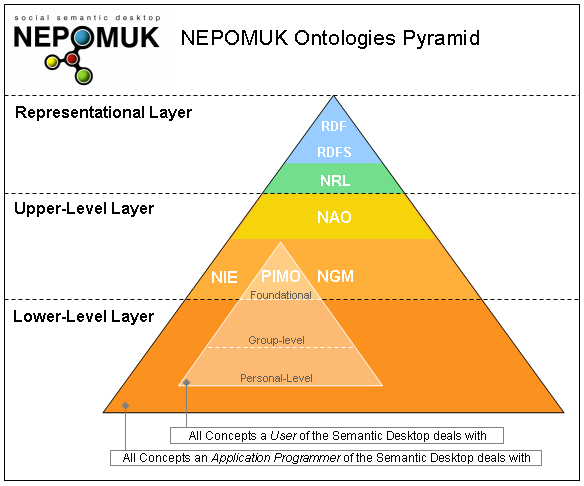
\includegraphics[width=1.00\textwidth]{images/roadmap.png}
	\caption{Integrated Ontologies}
	\label{fig:roadmap}
\end{figure}

The NEPOMUK Representational Language \textbf{NRL ontology}\footnote{\url{http://www.semanticdesktop.org/ontologies/nrl/}} builds the representational layer and the semantic
metadata axioms used to express PIMO. 
NRL is a meta-language comparable to OWL or RDF/S. 
The key characteristics of NRL are (on top of RDF/S) support for named graphs
in semantic statements, a notation for contextualized inference and semantics, 
and a selection of semantic relations (inverse, transitive, reflexive).

The NEPOMUK Information Element \textbf{NIE ontology}\footnote{\url{http://www.semanticdesktop.org/ontologies/nie/}} describes desktop elements such as address book entries, documents,
e-mails, appointments, pictures, and multimedia files.
The ontology discriminates between the representation (binary files)
and the information stored therein. 
PIMO reuses the classes of NIE and suggests how to integrate
and annotate vast personal spaces of information (PSI) expressed in NIE.

Annotations and tagging are represented in the NEPOMUK Annotation \textbf{NAO ontology}.
It represents change-dates, author, and other key metadata of documents.
NIE and PIMO both extend NAO. A part of NAO is the NEPOMUK Graph Metadata \textbf{NGM ontology} to annotate named graphs.

The PIMO ontology crosses two of the layers in the ontology pyramid, data related to PIMO can be divided into three smaller layers (also visible in Figure\ref{fig:roadmap}):
\begin{itemize}
	\item \emph{Foundational PIMO}: The PIMO ontology as such, as defined in this specification and accompanying NRL serialization. This includes the classes and properties of \emph{PIMO-upper} (see Section \ref{sec:pimoupper}), which work on the \emph{Upper-Level Layer} of NEPOMUK and everything else defined in the PIMO vocabulary. PIMO-upper is the same for every Semantic Desktop user and is valid in a global context.
	\item \emph{Group-level PIMO}: Domain ontologies that are shared within a group. They can be imported by users. A description is given in Section~\ref{sec:pimomid}.
	\item \emph{Personal-level PIMO}: The classes, properties, and Things created by an individual user. Also called \emph{user-PIMO}, this layer includes the data that is only relevant in the context of one individual.
\end{itemize}

\section{Examples}
\label{sec:examples}
A scenario is used to explain the ontology elements. A fictional persona, Claudia Stern, is our example user. She is working for EX-Ample Inc., a fictional company producing ``\textbf{Ex}treme Guitar \textbf{Ampl}ifi\textbf{e}rs'', and her current task is to organize a business trip to a meeting with guitarists and bass players in Belfast.

% taken from RDFS primer
For convenience and readability, this specification uses an abbreviated form to represent URI-References. A name of the form \texttt{prefix:suffix} should be interpreted as a URI-Reference consisting of the URI-Reference associated with the prefix concatenated with the suffix.

RDF graphs are written in N3/Turtle syntax. Examples serialized as RDF appear in this typesetting:
%\note{\emph{Knud}: I find the statement (Claudia user Claudia) very confusing. What's that supposed to mean? \emph{Leo}: that was garbage, we had it in the ontology before as an alternative to isDefinedBy.}
{\small
\begin{verbatim}
claudia:Claudia a pimo:Person;
 pimo:isDefinedBy claudia:PIMO;
 nco:hasEmailAddress <mailto:claudia@example.com> .
\end{verbatim}
}

\subsection{PIMO ontology and namespaces}
The ontology described in this document has this namespace:

{\small
\begin{verbatim}
Namespace:
http://www.semanticdesktop.org/ontologies/2007/11/01/pimo#
\end{verbatim}
}

During the lifetime of the NEPOMUK project (until Dec 2008), the PIMO ontology
and the according documentation may change, but the namespace will not change.
The namespace stays fixed to keep the necessary changes
of software implementations at a minimal level.
We have adopted this practice from other projects, which have applied it successfully. Examples are the W3C's  XSD datatypes (the recommendation changed in 2007, the namespace did not) or the FOAF project.

Throughout this document these ontologies and namespaces are used, also indicating their respective versions PIMO is building on:
{\small
\begin{verbatim}
@prefix rdf:  <http://www.w3.org/1999/02/22-rdf-syntax-ns#>.
@prefix rdfs: <http://www.w3.org/2000/01/rdf-schema#>.
@prefix nrl:  <http://www.semanticdesktop.org/ontologies/2007/08/15/nrl#>.
@prefix nao:  <http://www.semanticdesktop.org/ontologies/2007/08/15/nao#>.
@prefix pimo: <http://www.semanticdesktop.org/ontologies/2007/11/01/pimo#>.
@prefix ncal: <http://ont.semanticdesktop.org/ontologies/2007/04/02/ncal#>.
@prefix nco:  <http://ont.semanticdesktop.org/ontologies/2007/03/22/nco#>.
@prefix nfo:  <http://ont.semanticdesktop.org/ontologies/2007/03/22/nfo#>.
@prefix nie:  <http://www.semanticdesktop.org/ontologies/2007/01/19/nie#>.
@prefix nmo:  <http://www.semanticdesktop.org/ontologies/2007/03/22/nmo#>.

@prefix claudia: <http://www.example.com/people/claudia#> .
\end{verbatim}
}

\section{Creating Personal Information Models}
\label{sec:creatingPIMOs}
In this section, all key elements of the ontology are presented.
The order used reflects the steps a knowledge engineer will have to take to implement this recommendation.

\subsection{The User and their Individual PIMO}
\label{sec:pimo-user}
As a prerequisite to create a PIMO and Things inside the PIMO, each user needs a \emph{personal namespace}. The namespace is used as a prefix for all URIs minted for the user. Often these are namespaces using the HTTP URI scheme, but any RDF namespace can be used. The example namespace used in this document is \texttt{http://www.example.com/people/claudia\#} and is abbreviated with ``\texttt{claudia:}''.

\note{\emph{Knud}: In general, I would write all ontology elements in a different font. E.g., \texttt{pimo:Person}
\emph{Leo}: actually, I would like to write a script that, once this is converted
to HTML, replaces all ``pimo:NAME'' with HTML links to the ontology definition 
within the namespace.
\emph{Knud, 28/12:} unfortunately, there isn't always a namespace given. For now, I changed all ontology elements to monospaced font}

Users are represented as instances of the class \texttt{pimo:Person}. For each instance, a new URI is generated and a few key facts are represented to identify the user.
After the user has been instantiated, details such as email addresses are added by using terms from the NEPOMUK contact ontology, NCO. 
%\note{Knud: What do you mean by ``as the second object''? \emph{Leo}: fixed this, its a new resource.} 
In NCO, contact information connected to people is modeled as a complex resource, not as a simple literal:
%For the sake of simplicity, we used the URL \texttt{mailto:claudia@example.com} as identifier for this nco:EmailAddress resource.
{\small
\begin{verbatim}
claudia:Claudia a pimo:Person;
 rdfs:label "Claudia Stern";
 nco:hasEmailAddress mailto:claudia@example.com.

mailto:claudia@example.com a nco:EmailAddress;
 nco:contactMediumComment "work";
 nco:emailAddress "claudia@example.com".
\end{verbatim}
}

The second entity that needs to be represented is the \emph{Personal Information Model of the User}. It is connected to the user via the \texttt{pimo:creator} relation, and the user's namespace is added.
For Claudia this is:

{\small
\begin{verbatim}
claudia:PIMO a pimo:PersonalInformationModel;
  pimo:creator claudia:Claudia;
  nao:hasDefaultNamespace "http://www.example.com/people/claudia#";
  nao:hasDefaultNamespaceAbbreviation "claudia".
\end{verbatim}
}

\texttt{pimo:PersonalInformationModel} is a sub-class of \texttt{nrl:Ontology}, allowing more metadata to be added using NRL compliant standards. More about NRL metadata is described in Section~\ref{sec:nrlgraphs}. 
We further call a this instance of \texttt{pimo:PersonalInformationModel} of an individual a \emph{user-PIMO}. Claudia's user-PIMO is \texttt{claudia:PIMO}. As an abbreviation, it is also correct to write  ``Claudia's PIMO'' instead of ``Claudia's user-PIMO''.
\note{\emph{Knud, 28/12:} I'm confused by this term PIMO-user. It sounds as if it meant ``The user of the PIMO'', but it actually means ``The PIMO of the user'' --- correct? That's potentially confusing.} 
\note{\emph{Leo, 8/1:} reduce to ``user's PIMO'' and ``Claudia's PIMO''?}

\subsection{Things}
\label{sec:thing}
The PIMO ontology defines the basic class \texttt{Thing} for mental concepts. Every information element encountered in knowledge work by a user is represented as a Thing.
\note{\emph{Knud, 28/12:} Thing is inconsistently spelled with lower- and upper-case throughout the document.}
A Thing is a unique representation of an entity of the real world within one user-PIMO. On the PSI of a user, a real world entity can be represented in multiple data sources. For example, the person ``Dirk Hagemann'' may be author of an e-mail, described in an address book entry, and stored in a accounting tool, all part of the workspace of ``Claudia''. 
One instance of \texttt{pimo:Person} is created as unique \texttt{Thing} linking to these multiple representations, such as shown in Figure~\ref{fig:thing_vs_resource}.
\note{\emph{Knud, 28/12:} Yes, this is a Thing, but it is also a pimo:Person? Potentially confusing. \emph{Leo, 8/1:} changed the wording to speak of a Person}

\begin{figure}[htbp]
	\centering
		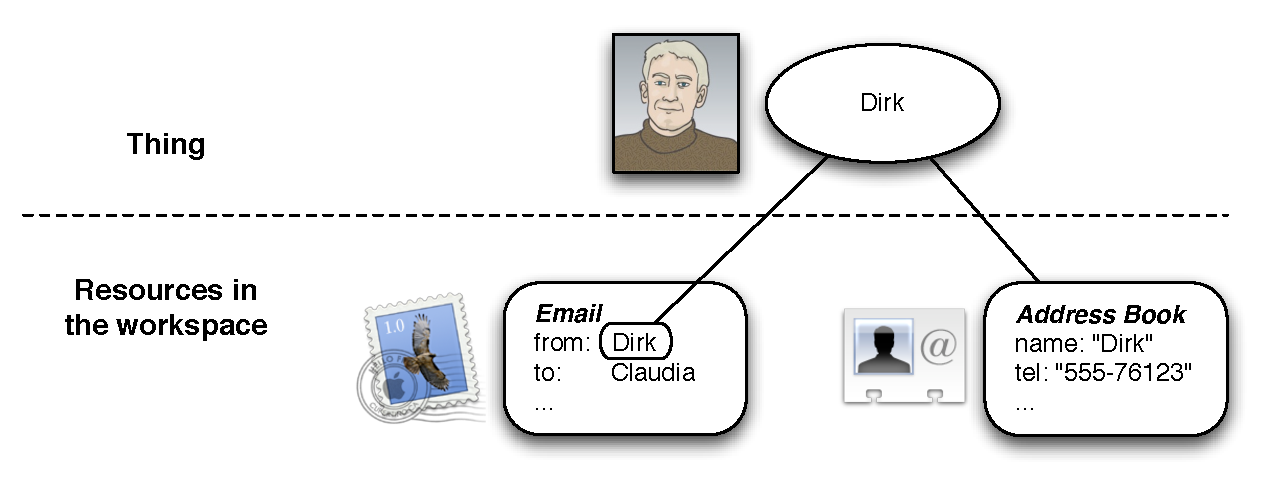
\includegraphics[width=1.00\textwidth]{images/thing_vs_resource}
	\caption{Thing and Resources}
	\label{fig:thing_vs_resource}
\end{figure}

An application handling a resource in the workspace can be aware that there may be a Thing representing the resource. For example, Claudia's e-mail client may examine the sender of an e-mail (Dirk) and search for the \texttt{pimo:Thing} that represents Dirk uniquely. Once the right Thing is found by the application, more information about Dirk can be discovered.

This principle includes all elements (\texttt{nie:InformationElement} and other RDF resources) in the user's \emph{Personal Space of Information (PSI)}. 
For each information element, a Thing in the user's PIMO must be created. 
The information element exists independent of the user, the same element can
be stored in multiple folders or data sources on one desktop, and also on other desktops and on the web. 
A Thing is the personalized view of \emph{one user} on this information element, independent of representation or storage location.

To be adequate, a PIMO of a user should contain all nameable entities known to the user,
but to be efficient, this representation should be restricted to the minimal data needed.
%Leo 29.7.2008: this is also explained later
% Identification is part of this minimal data, and \texttt{nao:identifier} provides the property for it.

\subsection{Connecting Things to the User's PIMO}
\label{sub:connectingThingsToPimo}
In a scenario of multiple connected semantic desktops, it will frequently occur that users import data from each other's desktop onto their own desktop.
It is therefore important to know which resources (primarily Things, but also Classes and Properties) were created by which user and originate from which PIMO. For this, the property \texttt{pimo:isDefinedBy} is used.

Continuing the example above, this property connects the Person to the PIMO in which it is defined.  This is mandatory for every defined Thing and allows applications to identify which elements are part of a user-PIMO and which are not\footnote{We intentionally did not only rely on NRL graphs to model the relation between the model and instances defined by it. A graph can only contain \emph{statements}, 
about, but not \emph{resources} as such.
To model that a resource is part of a PIMO, the \texttt{pimo:isDefinedBy} relation is a clear representation.
Additionally, named graphs can be used to declare what \emph{statements} are declared in a PIMO, see~\ref{sec:nrlgraphs}}.

{\small
\begin{verbatim}
claudia:Claudia pimo:isDefinedBy claudia:PIMO.
\end{verbatim}
}

An \texttt{isDefinedBy} property is also defined in RDFS, where resources can be connected to their defining ontologies, and is also discussed in the light of the OWL standard\footnote{\url{http://www.w3.org/2007/OWL/wiki/Syntax\#Declarations_and_Structural_Consistency}}. 
The semantics of \texttt{isDefinedBy} in PIMO is based on these, with the extension that we define it as a required property.

\subsection{Identification of Things}
\label{sec:identification}
A Thing \textbf{must} have an URI and \textbf{should} be described with properties that identify it. 
Identifiers allow to analyse information elements and find occurrences of the Thing.
For example, the person ``Dirk Hagemann'' is represented once as an instance of the class \texttt{pimo:Person} and identified using his e-mail address. 
The RDF descriptions of emails and documents can then be analysed to find resources that represent the same entity via this identifier. 
{\small
\begin{verbatim}
# The canonical Dirk
claudia:DirkHagemann a pimo:Person;
 pimo:isDefinedBy claudia:PIMO;
 nco:hasEmailAddress <mailto:dirk@example.com>.

# An e-mail in which Dirk #2 occurs
<imap://claudia@example.com/INBOX/1> a nmo:Mail;
 nmo:from <imap://claudia@example.com/INBOX/1#from>.

# Dirk #2, the email sender
<imap://claudia@example.com/INBOX/1#from> a nco:Contact;
 nco:hasEmailAddress <mailto:dirk@example.com>.
<mailto:dirk@example.com> a nmo:EmailAddress;
 nco:emailAddress "dirk@example.com".
 
# Dirk #3, as address book contact
<file://home/claudia/dirk.vcf#dirk> a nco:PersonContact;
 nco:nameFamily "Hagemann";
 nco:nameGiven "Dirk";
 nco:hasEmailAddress <mailto:dirk@example.com>;
 nco:photo <http://www.example.com/people/dirk/photo.jpg>.
 
\end{verbatim}
}

In this example, we see that the Person Dirk appears three times in this knowledge workspace. First, in the form of an instance of \texttt{pimo:Person}, as the canonical Dirk. Second, as sender of an e-mail and third as entry in an address book. Only one instance is the \texttt{pimo:Thing} representation of Dirk: \texttt{claudia:DirkHagemann}. The others are information elements representing the same entity.

\begin{figure}[htb]
	\centering
		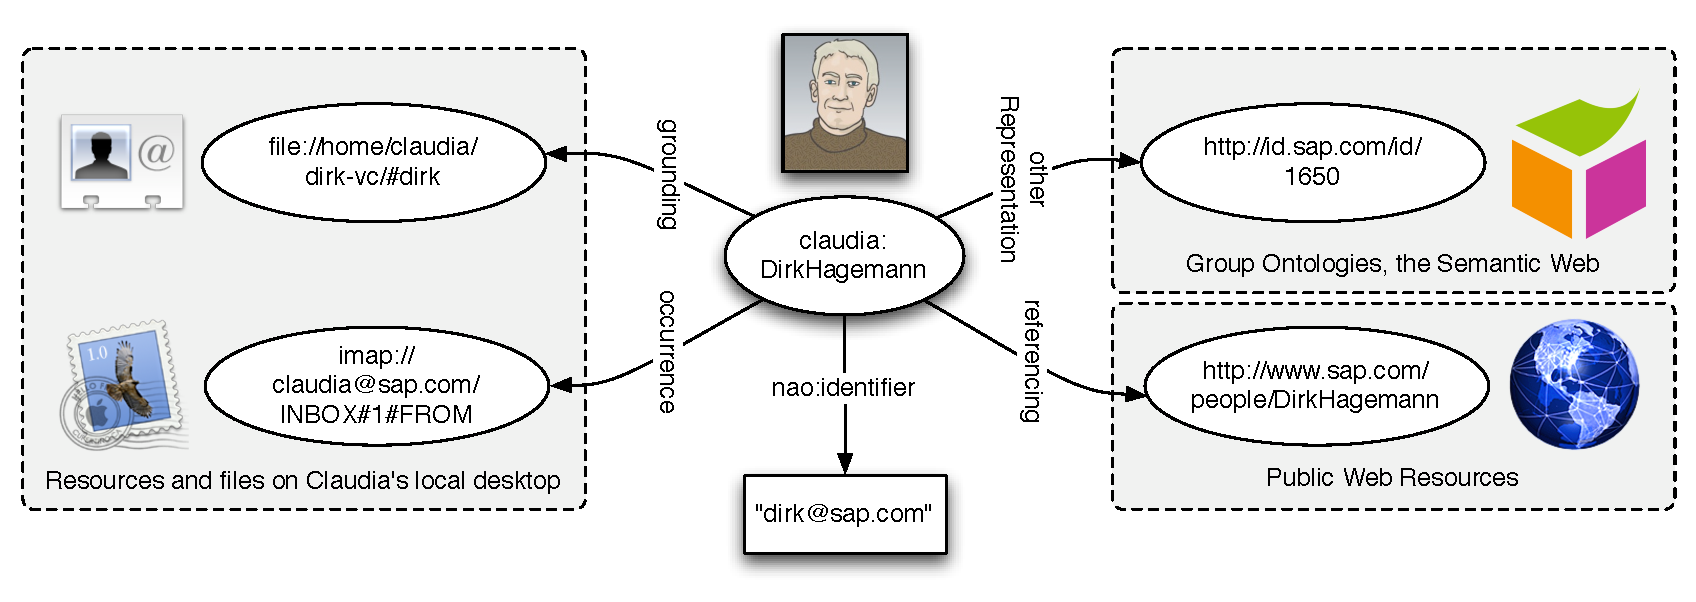
\includegraphics[width=1.00\textwidth]{images/identification}
	\caption{Different Identification Mechanisms}
	\label{fig:identification}
\end{figure}


%\note{\emph{Knud}: can one ``use'' an assumption? Leo: rephrased to ``is based on''}
To work effectively, PIMO is based on the \emph{Unique Name Assumption} (UNA). 
The UNA is a rule that declares two RDF resources with different URIs as different individuals. 
This is common in desktop applications (for example files with different names are different) and intuitive to grasp for users. But it is different from the OWL ontology language
%\note{\emph{Knud}: is OWL a system? Leo: its an ontology language}
where duplicate entries are common and the UNA is not enforced. 
PIMO is designed for personal systems, where an application has access to the complete model and can avoid duplicates before creating them.

To enforce the UNA, duplicate Things \textbf{must} be avoided. 
The crucial moment to do this is before creating a new Thing.
Things can either be created by the user manually or automatically by analysing existing native resources. In any case, before creating a new Thing, all existing Things have to be examined if a Thing with a same name or same identifying properties already exists. 
If an existing Thing is found, it \textbf{must} be reused. 
Immediately after creating a new Thing, identifying properties should be set to distinguish the Thing and avoid duplication. 
% fix to https://dev.nepomuk.semanticdesktop.org/ticket/498
Section \ref{sec:creatingthingalgorithm} further describes the complete process of creating things.

In the next paragraphs, essential identifying properties are described, an overview is given in Figure~\ref{fig:identification}.

\textbf{The primary identifier of a Thing is it's URI}. New URIs for Things \textbf{must} be generated using the namespace of the user as prefix and then a unique local name. 
Although the local name can be entirely a random string, we recommend to include the label in the URI for readability. When minting a new URI that clashes with an existing URI, a random element can be added to the new URI. A URI for Claudia Stern is:
\begin{verbatim}
claudia:Claudia
\end{verbatim}

\paragraph{NAO-Identifiers} Existing identification schemes based on NAO should be reused for this purpose by representing them with 
%\note{Knud: you say pimo:identifier here and nao:identifier in the example below. Which one is it?\emph{Leo}: its nao:identifier (28.8.2007).} 
\texttt{nao:identifier} and its sub-properties. 
If an identifier is found as meta-data of a native resource (usually an \texttt{nie:InformationElement}), the identifier \textbf{must} be copied to the Thing.
This allows others to match and identify the correct Thing when encountering the next information element.
Example identifiers are \texttt{nmo:messageId} for e-mails, \texttt{ncal:uid} for appointments, or \texttt{nexif:imageUniqueID} for images. 
Instead of using the plain \texttt{nao:identifier} property, these specific properties should be used or new sub-properties of \texttt{nao:identifier} created
\footnote{I.e. if you want to represent ISBN numbers and there is no property for them, create a new sub-property \texttt{isbn} of \texttt{nao:identifier}.}.
In this document, we assume that e-mail addresses can be used to identify persons.

\note{\emph{Leo}: this example is not good, as e-mail addresses are modeled 
differently in NCO. How else can we identify a person? \emph{Knud, 28/12:} I think we can't... :P}
\begin{verbatim}
# Copy all identifiers you can find about the Thing.
claudia:DirkHagemann a pimo:Person;
 nao:identifier "dirk@example.com".
\end{verbatim}

Identifiers consisting of multiple RDF statements cannot be captured using \texttt{nao:identifier}.
They are comparable to a primary key in a relational database consisting of multiple
columns. These \textbf{multi-key identifiers} \textbf{must} be merged into one \texttt{nao:identifier}.

\paragraph{Grounding Occurrence} The relation \texttt{pimo:groundingOccurrence} is used to link a Thing to an \texttt{nie:InformationElement} that has this Thing as primary topic. For example, the grounding for a person could be the entry in the address book describing the person. On the other hand, an e-mail with this person as the sender or recipient would normally not be a grounding occurrence. A Thing represents the mental concept, the \texttt{pimo:groundingOccurrence} links to existing Information Elements that are handled by existing applications. This is a key for reusing the features of these applications. 
The grounding occurrence can change, for instance if a file was moved and the URI of the Information Element changed, the grounding occurrence relation needs to be changed. 
A similar case happens when a file is uploaded to a shared workspace and not kept locally any more --- all annotations of the Thing stay the same (the URI of the Thing does not change), the Information Element changes.
Multiple values are allowed, this reflects the fact that the same Thing can be represented in multiple applications, and dependent on the work context, the user may want to open a different application. 
{\small
\begin{verbatim}
# Link to Dirk #3 from example above.
claudia:DirkHagemann a pimo:Person;
 pimo:groundingOccurrence <file://home/claudia/dirk.vcf#dirk>.
\end{verbatim}
}
\paragraph{Occurrence} The relation \texttt{pimo:occurrence} connects a \texttt{pimo:Thing} with a resource representing the same real world entity.
Facts about the occurrence are then also valid for the connected Thing. 
For example, if the person Dirk appears as sender of an e-mail, then the resource identifying the sender is an \emph{occurrence} of Dirk. 
Based on the occurrence relation, Dirk (the unique \texttt{pimo:Person}) is the sender of the given e-mail.
Occurrence relations are to be used on resources \emph{representing} the same entity in a different context, but not on resources \emph{mentioning} the entity. For example, it is not valid to say that an e-mail is an occurrence of a person, only the sender or recipient can be occurrences of a person.

%Not the e-mail as such is the occurrence, but the sender within. 
\note{\emph{Knud, 28/12:} Why is the e-mail as such not the occurrence? This should be explained, or not mentioned at all. 
Leo: done, removed sentence, replaced with longer explanation.}
Occurrences of a Thing can be found by searching for entities with the same identifying properties.

{\small
\begin{verbatim}
# Link to Dirk #2 from example above, 
# he occurs as sender of an e-mail
claudia:DirkHagemann a pimo:Person;
 pimo:occurrence <imap://claudia@example.com/INBOX/1#from>.
\end{verbatim}
}

Besides identification, both the \texttt{pimo:groundingOccurrence} and the \texttt{pimo:occurrence} relation have 
implications on data integration and affect semantic meaning of a Thing. 
This will be described later in Section \ref{sec:pimoVSnie}.

\paragraph{Referencing Occurrence} 
%\note{Maybe rename to indicatingOccurrence, closer to Topic Maps? Leo: I don't care, leave it as is.}
\label{par:referencingOccurrence}
A Referencing Occurrence is an indirect approach to identification. 
Annotating a Thing with an information element as \emph{referencing occurrence} states that the information element contains a description of the Thing.
Its primary topic must be the Thing.
The Thing is indirectly identified by the element, when two Things in different models share the same information element as referencing occurrence, they may be equal and could be matched. 
The following description is an adaption of XTM's subject indicators~\cite{XTM,Rath2003}.
The referencing occurrence is a kind of proxy for the Thing. Examples of referencing occurrences are:

{\small
\begin{verbatim}
claudia:DirkHagemann a pimo:Person;
 pimo:referencingOccurrence <http://www.example.com/people/DirkHagemann>.
 
claudia:ExampleInc a pimo:Organization;
 pimo:referencingOccurrence <http://www.example.com/>;
 pimo:referencingOccurrence <http://en.wikipedia.org/wiki/Example.com>.
\end{verbatim}
}

It should contain a human readable documentation describing the concept. The resource could be a document, ontology, video, audio, anything able to describe to a human what the concept is about. The resource is a reference to the concept of the Thing. 
A good example for a referencing occurrence is a wikipedia article.

A referencing occurrence describes the concept with the purpose of being widely used by ontologies. Consequently, it is important that the document describes exactly what concept it is about and what not. Even if the author works as accurately as possible, different people will never interpret a referencing occurrence 100\% the same way. However, the concept of referencing occurrences is worth using it, because it allows a shallow match of heterogenous information models, and because there is finally no alternative to it. 

\textbf{It is recommended to use wikipedia URIs as objects of referencing occurrences.} In contrast, URIs minted by \emph{DBPedia}\footnote{DBPedia is a Semantic Web representation of wikipedia and provides URIs for concepts, whereas wikipedia provides URIs for documents describing concepts. An example DBPedia URI is: \url{http://dbpedia.org/page/Berlin}} \textbf{must} be related using the \texttt{pimo:hasOtherRepresentation} relation.

\paragraph{Other Representation} 
\label{par:otherRepresentation}
The \texttt{pimo:hasOtherRepresentation} relation is used to connect \texttt{pimo:Things} with other representations of the same Thing in other Semantic Web ontologies. 
This can be the case with shared ontologies, such as company white page systems or Semantic Social Networking websites. 

The knowledge modeled should be compatible with the ontologies used by the user. An example for such other representation is\footnote{Using the URI scheme of the ECS University in our example domain. \url{http://id.ecs.soton.ac.uk/docs/}}:
\begin{verbatim}
claudia:DirkHagemann a pimo:Person;
 pimo:hasOtherRepresentation <http://id.example.com/person/1650>.
\end{verbatim}

Another example would be the city of Belfast where Claudia wants to travel to,
linked to the DBPedia entry about it:
\begin{verbatim}
claudia:Belfast a pimo:City, pimo:Tag;
  pimo:isDefinedBy claudia:PIMO;
  pimo:tagLabel "Belfast";
  pimo:hasOtherRepresentation <http://dbpedia.org/resource/Belfast>;
  geo:lat "54.5833333";
  geo:long "-5.9333333".
\end{verbatim}
The relation can be used both to identify Things by their other representations,
and to fetch more data.
In this example, the latitude and longitude are actually superfluous data,
as they can be retrieved from the other representation
in DBPedia.
Assuming Dirk also represents Belfast in his PIMO, but independent from Claudia,
but linking to the same DBPedia entry, algorithmically matching their different representations is straightforward.

\paragraph{Other Conceptualization}
To map user-generated classes to classes defined in other ontologies, the 
\texttt{pimo:hasOtherConceptualization} relation connects classes defined in a user's PIMO
with classes defined in domain ontologies. 
Classes defined in domain ontologies should be sub-classes of PIMO-upper classes, see Section \ref{sec:integratingontologies}. 

Implementations can use the \texttt{pimo:hasOtherConceptualization} to allow the user and algorithms
to map user--specific classes to classes defined in other ontologies,
without implying that there is a sub-class relationship.

\subsection{A Complete Example} 
A complete example for all different identification properties 
can now be built from the above annotations.

For Claudia, her co-worker Dirk Hagemann is identified and linked to occurrences like this:

{\small
\begin{verbatim}
# The canonical pimo:Person Dirk, 
# a pimo:Thing from Claudia's PIMO
claudia:DirkHagemann a pimo:Person;
 pimo:isDefinedBy claudia:PIMO;
 nao:prefLabel 'Dirk Hagemann';
 nao:identifier "dirk@example.com";
 pimo:occurrence <imap://claudia@example.com/INBOX/1#from>;
 pimo:groundingOccurrence <file://home/claudia/dirk.vcf#dirk>;
 pimo:referencingOccurrence <http://www.example.com/people/DirkHagemann>;
 pimo:hasOtherRepresentation <http://id.example.com/person/1650>.
 
 
# An e-mail in which Dirk #2 occurs
<imap://claudia@example.com/INBOX/1> a nmo:Mail;
 nmo:from <imap://claudia@example.com/INBOX/1#from>.

# Dirk #2, as email sender
<imap://claudia@example.com/INBOX/1#from> a nco:Contact;
 nco:hasEmailAddress <mailto:dirk@example.com>.
 
<mailto:dirk@example.com> a nmo:EmailAddress;
 nco:emailAddress "dirk@example.com".
 
# Dirk #3, as address book contact
<file://home/claudia/dirk.vcf#dirk> a nco:PersonContact;
 nco:nameFamily "Hagemann";
 nco:nameGiven "Dirk";
 nco:hasEmailAddress <mailto:dirk@example.com>;
 nco:photo <http://www.example.com/people/dirk/photo.jpg>.
\end{verbatim}
}

This allows implementations to:
\begin{itemize}
	\item identify the Thing when found occurring in documents,
	\item open a grounding occurrence to see the Thing within an existing desktop application (i.e. the address book entry for a person),
	\item match this Thing with other representations via the same referencing occurrence,
	\item use the other representation from the company's white pages to show additional data about the Thing.
\end{itemize}

The \texttt{pimo:occurrence} link is the generic basis, \texttt{pimo:groundingOccurrence} and \texttt{pimo:hasOtherRepresentation} are sub-properties of it. This data should be generated automatically and unsupervised. 
Adding identifying properties to a Thing helps to find more occurrences and therefore more information about it.

\subsection{Labels and Names of Things}
\label{sec:labelling}
To label Things, we recommend the NEPOMUK Annotation Ontology (NAO) vocabulary
and extended it.
NAO defines properties for the \emph{preferred label}, \emph{multiple alternative labels}. PIMO defines \emph{tag labels} as unique names for unique Tags.

\paragraph{\texttt{nao:prefLabel}} \textit{A preferred label for a Thing}.
This property \textbf{must} be applied to every instance of \texttt{pimo:Thing} (or its sub-propery \texttt{pimo:tagLabel}).
It can be used by applications to represent the Thing with a textual label and should be human-readable. There must only be one \texttt{prefLabel} per Thing (mincardinality and maxcardinality should be one)\footnote{These restrictions are not explicitly noted in the RDF description of the property, as NRL does not support property restrictions for classes.}.

\paragraph{\texttt{pimo:tagLabel}} \textit{Defines a unique personal label for a Thing, which then is also a Tag.}
The label \textbf{must} be unique within
the scope of a user. 
If both are set, \texttt{pimo:tagLabel} and \texttt{nao:prefLabel} of a resource \textbf{must} have the same value. 
It is a sub-property of \texttt{nao:prefLabel} and of \texttt{nao:personalIdentifier}.

\textbf{Tag labels are the \textbf{recommended} way to label and identify Things that are used for classification}.
As they are unique and human-readable, they \textbf{may} be used for multiple application scenarios such as wikis, tagging, or matching terms found in free-text.
Naming a Thing with a \texttt{pimo:tagLabel} gives the Thing a second type, \texttt{pimo:Tag}, which indicates that the Thing should now be considered part of the user's tagging system, see Section~\ref{sec:tagginginpimo}. 
\note{\emph{Knud, 28/12:} I don't understand: should the two properties be the same or not? Leo: recommended they should be the same.}

\paragraph{\texttt{nao:altLabel}} \textit{An alternative label alongside the preferred label for a Thing.} These are alternative spellings, translations, nick-names.
%\note{\emph{Knud, 28/12:} Spelling Mistakes? Leo: removed this, replaced with nick-names}
Implementations can use these labels to find Things when the user enters a text in a search box or when analysing free text.
If a Thing has occurrences, the labels of occurrences \textbf{should} be copied as alternative labels to the thing.

In combination, these labelling techniques allow applications to clearly label Things in user interfaces but also to lookup for Things based on alternative names. For our example, these are:

\begin{verbatim}
claudia:DirkHagemann a pimo:Person;
# preferred label when shown
 nao:prefLabel "Dirk Hagemann";
# a nickname for Dirk
 nao:altLabel "hacki";
# a common misspelling
 nao:altLabel "Dirck Hagemann";
# the personal identifier and tag label, 
# Attention: this requires the class pimo:Tag
 pimo:tagLabel "Dirk Hagemann".
\end{verbatim}

Additionally, visual cues (icons, images, thumbnails) can be attached by using NAO symbol relations:
\begin{itemize}
	\item \texttt{nao:hasSymbol}
	\item \texttt{nao:prefSymbol}
	\item \texttt{nao:altSymbol}
\end{itemize}

\subsection{Textual description of Things}
\label{sec:freetextdescription}
To describe Things with a free-text, the simple \texttt{nao:description} property should be used. This allows users to add a (possibly searchable) description of the Thing in a simple way. The description string value should contain no format markup but be a plain text.

For more complex free-text descriptions of Things, the property \texttt{pimo:wikiText} is reserved. 
Formatting (font-weight, italics) and linking to other pages is supported
in this property, implementers may use the \emph{Wiki Interchange Format}
\footnote{\url{http://semanticweb.org/wiki/Wiki_Interchange_Format}}
as syntax, or RDFa\cite{rdfaprimer}.

\subsection{Rating and Ranking Things} % (fold)
\label{sec:ratings}
\textbf{Ratings of Things} can be expressed using \texttt{nao:numericRating}.
For numericRating, the range of values \textbf{must} be within $[0..10]$ (inclusive)
\footnote{Implementers may wonder why the range is not standardized as $[0..1.0]$. The recommended range is based on an implementation decision taken in KDE.}. 
A value of '0' is interpreted as not set, a rating of 1 a \emph{bad rating} and a rating of 10 a \emph{good rating}. 
Furthermore, resources can only be given at most one numeric rating, thus the maximum cardinality is 1.
Applications \textbf{may} partition the values into discrete ratings (such as 2, 4, 6, 8, 10 to represent the semantics of ``5 star ratings'').

The rating values may and should be used for \emph{ranking} of Things
and filtering. A populated PIMO contains thousands of Things,
user interfaces should use the \texttt{nao:numericRating} values
to filter out low-ranked resources and highlight high-ranked
resources.
Implementations \emph{can} set the \texttt{nao:numericRating} 
values automatically to computed values.
% Alternatively, implementations can set an automated rank and
% compute the overall rank using auotmated rank + nao:numericRating


% paragraph ratings (end)

\subsection{Modelling Time}
In PIMO, no special treatment of time is modeled. 
We are aware that representing points in time, durations, and other periods of time
is an important aspect of ontologies. 
We recommend to use the XML Schema Datatypes
to represent time. 
There, ISO 8601 is recommended. Timezones must be handled according to this standard,
encoded inside the literal value\footnote{For a detailed representation of time events, refer to the NIE documentation, where timezones are discussed (\url{http://www.semanticdesktop.org/ontologies/2007/04/02/ncal/\#sec-tzd}).
NIE represents time using the NcalDateTime class and its properties 
date, dateTime, ncalTimezone. Timezones are represented using a Timezone class,
that is inspired by RFC 2445.}.

Periods of time can be represented using sub-classes of the abstract class
\texttt{pimo:ProcessConcept} which represents lasting processes such as events
or projects. For durations that last a number of days or months, we recommend to use the standardized XML datatypes\footnote{The XS namespace is \texttt{http://www.w3.org/2001/XMLSchema}, but the two duration datatypes are defined in the XPath recommendation in 2007, see \url{http://www.w3.org/TR/xpath-functions/\#dt-dayTimeDuration}}:
\begin{itemize}
	\item \texttt{xs:dayTimeDuration} for durations measured in days, hours, and minutes.
	\item \texttt{xs:yearMonthDuration} for durations measured in months and years
\end{itemize}
Implementers are free to use either the XSD types or sub-classes of 
\texttt{pimo:ProcessConcept}.

There have been issues with other notations of duration and therefore the W3C Semantic Web Best Practices and Deployment Group published a note\footnote{\url{http://www.w3.org/TR/swbp-xsch-datatypes/\#section-duration} Since XPath 2.0 has become a W3C recommendation in January 2007, this note is partly obsoleted.} to restrict durations to these values. 

\subsection{Representing Modification and Change Dates}
\label{sec:changedates}
The change and creation dates of Things are important metadata for personal information management applications. Knowing about recent changes is an important cue for users to retrieve documents. Many applications offer the feature to show recent changes or filter by them. Consequently, it has to be straightforward, simple, and fast to query for the modification dates. 

The NAO properties \texttt{nao:created}, \texttt{nao:modified}, and \texttt{nao:lastModified} \textbf{shall} be used to track the change dates of Things. 
Creation and modification allow only one, modification allows multiple date values.
Created and lastModified values \textbf{must} be set for each Thing,
at least one modified value \textbf{must} be set.
These values are intended for resources of type \texttt{pimo:Thing}, \texttt{pimo:Association}, \texttt{rdfs:Class}, and \texttt{rdf:Property} when created by the user.
\note{\emph{Knud, 28/12:} Why is this not enforced? 
\emph{Leo, 8/1:} mandatory is better anyway, CHANGED}

Example:
\begin{verbatim}
# Represent modification dates of a Thing
claudia:DirkHagemann
  nao:created "2007-10-26T15:23:01";
  nao:modified "2007-10-26T15:23:01";
  nao:modified "2007-10-29T08:04:30";
  nao:lastModified "2007-10-29T08:04:30".
\end{verbatim}

The \textbf{semantics} of these dates is that the description of the Thing has changed, facts about the Thing have been added, removed, or modified. Changes to \texttt{pimo:objectProperty} (\texttt{pimo:related}, \texttt{pimo:hasTag}, etc.) or \texttt{pimo:datatypeProperty}  (\texttt{name}, \texttt{address}, \texttt{label}, etc.) imply such a modification. 
Included are also changes to the labels (\texttt{nao:prefLabel}, \texttt{nao:altLabel}, \texttt{pimo:tagLabel}).
Modification of any other statement (such as \texttt{pimo:definedBy}, \texttt{nao:modified}) do not imply a modification nor a change of dates.
As current RDF stores a priori do not support automatic tracking of changes, applications have to implement housekeeping of these dates, or use services for tracking.
\footnote{The value of lastModified is redundant as it could be computed by sorting the modified dates during query time, but this is not possible without nested SPARQL queries, a $max()$ function, and grouping, none of these part of the SPARQL standard. The stores that support such non-standard operations still need time to compute the value. As the last modification date is very important for applications to assist users finding information, the redundancy is intended.}

\note{\emph{Knud, 28/12:} I removed a paragraph here (still commented in the source), because I think it doesn't belong here. This document is a specification, not a scientific document. Leo: OK}
%In RDF and using named graphs, there are more ways of representing change dates. It is possible to remember the date when a graph changes, implying that all triples inside the graph have changed. Based on this, it can be implied that all resources described in these triples have changed. But there is no formal relation between a resource and a graph that describes it. For example a class being used as object of a rdf:type relation, does this express that the class has changed? Or a resource being annotated in a reification statement. Changes to the graph may not directly relate to changes of the resource in the view of the user. 
%Also, as dates are a very prominent fact needed for data visualization and search result ranking, a graph-based approach will not provide satisfactory answer times
%\footnote{To select a date using graph metadata, a query for the context of all statements where a resource is either in subject or object role and the change date of these contexts would be needed.}.

\subsection{Setting the Class of a Thing}
\label{sec:classofthing}
All Things are of type \texttt{pimo:Thing} or one of its sub-classes. The PIMO ontology itself defines several sub-classes such as \texttt{pimo:Person} or \texttt{pimo:Organization}. If these are not specific enough, the user can either create new sub-classes manually (see Section \ref{sec:customontology}), or import group-level ontologies (Section~\ref{sec:integratingontologies}).

As a rule of thumb, the question to be answered by assigning the class is ``\emph{What is this Thing?}''.
In comparison to OWL, where classes are commonly based on the properties of the object (``vegetarians are entities not eating flesh'') , classes represent the type (the \emph{nature}) alone. 
\note{\emph{Knud, 28/12:} idea: paragraphs such as this should be marked as ``suggestion for use''. Again, they don't really belong in a specification.
\emph{Leo, 8/1:} This paragraph is explanatory of the idea of classes in comparison to OWL, where most things are modeled as ``does this thing belong to a class or not'' Its important to have it. Cutted it, reworded it to refer to OWL. DONE?}
%For the concrete example of ``importance'', we recommend using the property \texttt{nao:numericRating} or by using part-of relations like ``this Thing is part of the collection of important things''.
%To model collections of things that share a common property (such as ``important Things''), the class \texttt{pimo:Collection} is provided.

It is also recommended to only use one explicit class for a Thing. The wish to add multiple classes is often an indication that some classes can be better modeled using relations. 
For example, it is recommended to use a datatype property \emph{``is this person a vegetarian? yes or no''} and explicitly set it instead of assigning a sub-class of Person called \emph{Vegetarian}.
If Things with two classes are needed (for example, if something is both a ``Car'' and a ``Locatable'') then the preferred way is to change the class model (make Car a subclass of Locatable or create a new class ``LocatableCar'' with both as superclass) than to add both types to one Thing. Nevertheless, it is not forbidden to add two types.
%Superclasses are inferred implicitly, and are not affected by this recommendation.

When a Thing has occurrences that are expressed in the NEPOMUK Information Element ontology (NIE), suitable mappings from NIE classes to PIMO classes are available in a mapping file
\footnote{\url{http://www.semanticdesktop.org/ontologies/2007/11/01/nietopimomapping.rdf}}.

\subsection{The PIMO-upper ontology}
\label{sec:pimoupper}
PIMO contains an \emph{upper ontology} for basic concepts in Personal Information Management (PIM):
Person, Location, Event, Organization, Topic, Document, Time. They are modeled
to answer basic questions about a Thing:
\begin{itemize}
	\item Who is associated? Person
	\item Where is this? Location
	\item When is it? Time
	\item What is it about? Topic
\end{itemize}
% addressing the ``foundational'' part of figure 1
The classes are the \emph{foundational part} of PIMO in the \emph{Upper-Level Layer} of the overall NEPOMUK ontologies as shown in~\ref{fig:roadmap}.
This level serves as integration point for PIM applications,
in the broader perspective of the Semantic Desktop, the classes can serve as upper classes for group-- and domain--level ontologies (see Sect.~\ref{sec:integratingontologies}).

\subsection{Classes in PIMO-Upper}
\label{sec:pimoUpperClasses}
The classes have been defined based on related ontologies, a user study, and several software prototypes that have been evaluated. Figure~\ref{fig:upperclasses} gives a rough overview of the available classes.

\begin{figure}
	\centering
		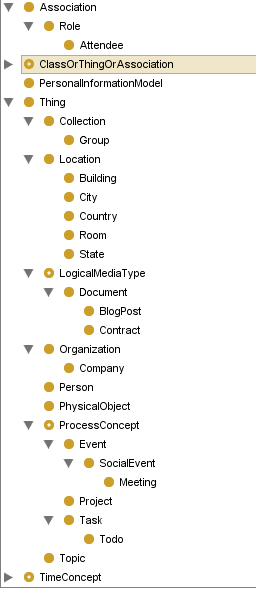
\includegraphics{images/upperclasses.png}
		\caption{Classes in PIMO-Upper}
	\label{fig:upperclasses}
\end{figure}

\begin{description}
%
%    NOTE !!!!!!!!!!!!!!!!!!!!!!!!!!!!!!!
%    These are copied from the ontology, and if not, the
%    descriptions have to be the same in the ontology and here.
%
	\item[Thing] The root class of the upper ontology. Every entity that can be in the direct attention of the user is a Thing.
	\item[Collection] A collection of Things, independent of their class. The items in the collection share a common property. Several usability studies showed that collections are important for PIM. It is recommended to either use the \texttt{pimo:hasPart} or the \texttt{pimo:isTagFor} relation to connect a collection with the Thing it contains\footnote{A Risk Of Change: A clear recommendation to either property may follow in future versions}.
	\item[Group] A group of Persons. They are connected to each other by sharing a common attribute, for example they all belong to the same organization or have a common interest.
	\item [Location] A physical location. Sub-classes are modeled for the most common locations humans work in: Building, City, Country, Room, State. This selection is intended to be applicable cross-cultural and cross-domain. City is a prototype that can be further refined for villages, etc.
	\item [LogicalMediaType] MediaConcepts are logical media types (e.g., a book, a contract, a promotional video, a todo list).  The user can create new logical media types dependent on their domain: a salesman will need MarketingFlyer, Offer, Invoice while a student might create Report, Thesis and Homework.
	\item [Organization] An administrative and functional structure (such as a business or a political party).
	\item [Person] Represents a person. Either living, dead, real or imaginary. In this regards, similar to \texttt{foaf:Person}.
	%\item [PhysicalObject] An object of interest in the physical world. \note{\emph{Knud}: if there is a physical object, how about an abstract object? Love? Language?
%\emph{Leo}: correct. I see a problem with Organozations and Topics, they have
%an overlap with AbstractObject. This can lead to a longer discussion...
%	we should consult sumo. I added this as an open issue at the end.\ref{issue:abstractobject}}	
%	It can be touched, it is concrete and it is of interest to the user. Examples are cars, tables, products and goods of business interest.
	\item[ProcessConcept] Concepts that relate to a series of actions or operations conducing to an end. Sub-classes are defined for Event, SocialEvent, Meeting, Project, and Task.
	\item[Topic] A topic is the subject of a discussion or document. Topics are distinguished from Things in their taxonomic nature, examples are scientific areas.
	\item[Tag] Tag is an abstract marker class to specify which Things in the user's PIMO should be considered useful tags in a tagging system. All Topics are Tags (Topic is a subclass of Tag). Implementations should support the user by using a useful set of Things as Tags, see Section~\ref{sec:tagginginpimo}.
\end{description}

These classes are intentionally kept generic. More specialized ontologies should be used for certain domains of application, see Section~\ref{sec:integratingontologies}. The classes of these ontologies are then  sub-classes of upper ontology classes. 

\subsection{Describing Things with Attributes and Relations}
\label{sec:describingthings}
Conventional RDF statements are used to describe Things. Predicates have to be defined as \texttt{rdfs:Properties} according to the NRL standard. Alternatively, it is also possible to use properties from other modeling languages like OWL or RDFS although we do not encourage this without a proper mapping of existing ontologies to PIMO (see~\ref{sec:integratingontologies}).

Properties that are intended to be editable and visible to end users \textbf{must} be sub-properties of either \texttt{pimo:datatypeProperty} or \texttt{pimo:objectProperty}.

Many NIE and NAO properties can be used from PIMO Things, see Section~\ref{sec:usingnieinpimo}. 

\subsection{Generic Properties in PIMO-Upper}
\label{sec:genericproperties}
The PIMO-upper ontology contains basic relations between Things and a few core attributes for identifying them (described above in Sect.~\ref{sec:identification}). 
These sub-properties of \texttt{pimo:objectProperty} are:
\begin{description}
  \item [\texttt{pimo:related}] is the most generic relation, giving no further indication how Things may be related. Related is defined to have itself as inverse property, 
  it is indirectly a \texttt{nrl:SymmetricProperty}, but does not inherit this attribute to sub-properties. Sub-properties can be asymmetric, depending on the inverse-of relation they define.
	\item [\texttt{pimo:hasPart}] and \texttt{pimo:partOf} model partitive relations. They are inverse. Neither is transitive, because part-of relations used for modelling in the domain of Personal Information Management are vague due to the many contexts of interpretation (a hotel may be part of a trip plan, a trip plan part of a project, but this does not indicate the hotel to be part of the project).
	\item [\texttt{pimo:hasTag}] and \texttt{pimo:isTagFor} connect a Thing of interest with a Tag characterizing it. For example, a meeting can have a project as a tag, or a document has a meeting as a tag, when the goal of the meeting is to discuss the document. After the meeting, the meeting minutes are a new Thing having the meeting as a tag. This is not restricted to meetings but also an organization or a person can have a certain technology as a tag to express that they are working on the topic described by the tag. The relation is not transitive, not symmetric. It is not asymmetric because a thing A may have thing B as tag, and B also A, if both are tags. The range of the \texttt{pimo:hasTag} relation is restricted to the class \texttt{pimo:Tag}. Topic is a subclass of tag. See Section~\ref{sec:tagginginpimo}.
\end{description}

Implementers may use these generic properties directly, or create sub-properties of them
or sub-properties of the more generic \texttt{pimo:objectProperty}.
The main reason to have the generic properties is the semantic meaning of the relations,
which can help to create user interfaces or model domains. 
Ontology authors can ask themselves ``does a new property model a part-of relation or not, does it assign a thing with a topic, or is it a generic relation?'' and then extend one of the generic properties.

For these generic relations, specialized sub-properties are defined when used on specific  classes in the PIMO upper ontology.

\subsection{Refined properties in PIMO-Upper}
\label{sec:pimoupperrelations}
Additional to the above relations, semantically interesting relations between PIMO upper classes are modeled. Especially those which can be used as symmetric or transitive relations for inference.

\begin{description}
	\item[\texttt{pimo:subTopic}] and \texttt{pimo:superTopic} relate Topics to each other. As Topics are an important mean to organize document collections based on a taxonomy, these two predicates are defined. They are inverse of each other and transitive.
	\item[\texttt{pimo:hasOrganizationMember}] and \texttt{pimo:isOrganizationMemberOf} are relations connecting a Person to an Organization.
	\item[\texttt{pimo:hasLocation}] and \texttt{pimo:isLocationOf} relate a locatable Thing with its Location. Locatable is an abstract sub-class of Thing.
	\item[\texttt{pimo:containsLocation}] and \texttt{pimo:locatedWithin} relate two locations within each other. Note that for geographic locations representing a physical space, inclusion is transitive.
\end{description}

\subsection{Tagging Things with Tags}
\label{sec:tagginginpimo}
% Say that PIMO is intended to work as an ontology, but also as a tagging system. When tagging e-mails or other elements, the name of the used tag must be unique. This is to be compatible with existing tagging systems, and to simplify the model. Intended use of TAG is to build a tag-cloud and organization system for the user's documents. Say that all topics are tags and are also arranged in a hierarchy (see next section). Recommend which classes make good tags: classes that exist for a longer time and can be used to classify many documents: topic, collection, group, city, person, organization, project. Say why it won't work without pimo:Tag. The classification system must be smaller than the document collection, to optimize retrieval.
The generic properties described in the last Sections show how Things can be related to each other.
An important aspect of PIMO is to classify Things using ``Tags''. 
Compared to normal PIMO Things, \emph{Tags} have one important additional restriction to make them compatible with Tags from other tagging system (folksonomies and Topic Maps):
\begin{itemize}
	\item The label of a Tag is unique, within the scope of one Personal Information Model.
\end{itemize}
Using Tags, PIMO can be used similar to an existing tagging system.

To extend a Thing to become a Tag, add the type \texttt{pimo:Tag}:
\begin{verbatim}
# The Person Dirk
claudia:DirkHagemann
  a pimo:Person;
# also a Tag
  a pimo:Tag;
# Must define the required pimo:tagLabel
  pimo:tagLabel "Dirk Hagemann".
\end{verbatim}
The \texttt{pimo:tagLabel} is required for all instances of \texttt{pimo:Tag}, and as it is a subproperty of \texttt{nao:prefLabel}, it can replace an existing prefLabel.
The \emph{intended use of Tags} is to build a clear category system for the user's documents. 
Once a Thing is \emph{tagged}, it can be retrieved by finding first the Tag, and then Things associated with the Tag.
A user's Tags are good candidates as first entry points to explore a data space, they can be visualized in a tag cloud or an alphabetical list. Tags can be clustered by type (each has an additional PIMO type), and by hierarchy (Tags can be organized in a part-of hierarchy, Topics are organized in a subTopic hierarchy).

To be useful as classification system, there should be a limited number of Tags to classify the potentially larger amount of documents. 
Examples are Things which exist for a longer period of time and Things that are of much importance to the user. 
Implementations \textbf{should} provide means to use the following as Tags.
\begin{itemize}
	\item All \textbf{Topics} can be considered Tags. This is expressed by the fact that Topic is a subclass of Tag.
	\item \textbf{Collections} work well as Tags, the act of putting something into a collection can be considered an act of tagging.
	\item A \textbf{person}.
	\item A \textbf{group of persons}. 
	\item A \textbf{city}, as there is a limited number of cities a person interacts with. 
	\item \textbf{Projects} are defined as an ``enterprise carefully planned'', the planning and execution of a project may involve tagging many Things as belonging to the project.
	\item A \textbf{task}, as documents may be needed to fulfill the task.
	\item An \textbf{organization} to classify to which organization a person belongs or by which organization a document was published.
\end{itemize}
The process of using an existing Thing as Tag \textbf{may} be automated. For example, a user searching for a possible Tag for a document should be able to pick from a list of existing Tags, and additionally search for Things of the above type to convert them to a Tag (such as a ``more Tags'' button). 
The conversion from Thing to Tag \textbf{may} then be automated and not visible to the user.

Tagging a document is illustrated in the following example, for more details refer to Section~\ref{sec:taggingfiles}.
\begin{verbatim}
claudia:BelfastMeetingPackage a claudia:MeetingPackage, pimo:Tag;
  pimo:tagLabel "Belfast Meeting Package".

claudia:BelfastBusTimetable a pimo:Document;
  pimo:groundingOccurrence <file://home/claudia/doc/tripplan.pdf>;
  pimo:hasTag claudia:BelfastMeetingPackage.
\end{verbatim}

In general, it should be avoided to use \texttt{pimo:Document} instances as Tags.
Typically the amount of documents is high, making them less useful as categorization scheme compared to the above mentioned Thing classes. 
The reason to introduce Tags in PIMO is to allow implementers to separate between categorization scheme and annotated instance base (which is usually a document corpus).
Without a class to mark Tags, it would not be possible to restrict the \texttt{pimo:tagLabel} predicate to a minimum cardinality of one, and also Topics could not automatically be defined as Tags.

\subsection{Topic Hierarchies}
\label{sec:topichierarchies}
% say that PIMO is a taxonomy system comparable to SKOS. The hierarchical ordering of Topics is important to organize the system. Hierarchies are also used to allow semantic search on subtopic structures. add rules.
The methodologies so far allow the description of individual Things with labels, properties, classes, and Tags. 
Besides the view on individuals, their place inside an overall organization scheme of the user can be important --- where is a Thing located in a hierarchy? 
Things can be placed in a hierarchy using the \texttt{pimo:hasPart} relation. 
In an overall hierarchy, the part relation can be confusing, as Things both have a class and can be part of something. For example, \emph{workpackage 2} is \emph{part of } the \emph{CID project}. In a combined hierarchy including class and part-of relations, it would appear at two positions: as instance of workpackage and as part of CID. 

To simplify the system for novice users, it is \textbf{recommended} for implementers to support a \emph{Topic Hierarchy}, where hierarchical part-of structures are shown to end-users. The semantic ``is-a'' relations \textbf{should} be hidden in the Topic hierarchy.
This allows users to model parts of their PIMO as taxonomy.
\begin{itemize}
	\item Each instance of \texttt{pimo:Topic} \textbf{must} either have a \texttt{pimo:hasSuperTopic} relation to another Topic or be defined as root Topic using \texttt{pimo:hasRootTopic}.
	\item All Topics \textbf{must} be connected (indirectly or directly) to a root Topic, or be a root Topic themselves.
	\item User interfaces \textbf{should} render Topics using the hierarchical structure.
	\item Cycles in the super-topic structure are allowed but \textbf{should} be avoided.
	\item A Topic can have multiple super Topics, PIMO allows poly-hierarchical structures.
	\item The \texttt{pimo:subTopic} and \texttt{pimo:superTopic} relations are defined \emph{transitive}. 
	\item When displaying Topics in hierarchical user interfaces, the transitivity of \texttt{pimo:subTopic} \textbf{should} not be inferred. The user experience should be the same when modelling and when browsing the hierarchy.
	\item When searching for Things using the \texttt{pimo:hasTag} relation, the transitivity of \texttt{pimo:subTopic} \textbf{should} be inferred, see below.
\end{itemize}

To support \emph{semantic search} in Topic hierarchies, the following rule for tagging does apply when searching for Things using the hasTag relation (for a detailled description, see Section~\ref{sec:pimorules}):
\begin{verbatim}
CONSTRUCT 
{?x pimo:hasTag ?B.} 
WHERE 
{?x pimo:hasTag ?A. 
?A pimo:superTopic ?B.}
\end{verbatim}

The hierarchical structure of Topics in PIMO is comparable to the modeling in SKOS\cite{SkosStandard}. The \texttt{pimo:subTopic} relation is equivalent to \texttt{skos:narrowerTransitive}.
PIMO requires all Topics to be connected to root Topics, SKOS does not require this in the semantics of \texttt{skos:hasTopConcept}.

\subsection{Creating Personalized Classes and Properties}
\label{sec:customontology}
The predefined classes and properties are intended as a generic basis to be extended.
The user can always create new classes and property types, or existing ontologies can be imported (see Section~\ref{sec:pimomid}).
A number of requirements apply:
\begin{itemize}
	\item The superclass has to be \texttt{pimo:Thing} or a sub-class.
%	\item The property pimo:isDefinedBy has to be set to express that the user created the % class.
	\item The class has to be labelled with \texttt{nao:prefLabel}.
	\item The class has to be related to the user's PIMO with \texttt{pimo:isDefinedBy}.
\end{itemize}

Similarly for custom properties:
\begin{itemize}
	\item The property has to be labelled with \texttt{nao:prefLabel}.
	\item The property has to be related to the user's PIMO with \texttt{pimo:isDefinedBy}.
\end{itemize}
For properties that relate two things, the following applies:
\begin{itemize}
  \item The property \textbf{must} be a sub-property of \texttt{pimo:objectProperty} (either directly or indirectly via inference).
	\item The super-property \textbf{should} be one of \texttt{pimo:related}, \texttt{pimo:hasTag}, \texttt{pimo:isTagFor}, \texttt{pimo:hasPart}, or \texttt{pimo:partOf}.
	\item An inverse property \textbf{must} be defined. Inverse properties define the semantic meaning in both ways, which is required for 
user interfaces showing relations.
\end{itemize}
For custom properties that have \emph{a literal or datatype as range} the following applies:
\begin{itemize}
  \item They must be a sub-property of \texttt{pimo:datatypeProperty}.
  \item Inverse properties should not be defined (as Literals cannot be subject of statements, inverse does not apply anyway).
\end{itemize}

For all custom-created properties and classes, 
modification dates \textbf{must} be set.

\subsection{Collections of Things}
\label{sec:collections}
In Personal Information Management, grouping multiple Things into one collection is a crucial feature. Today's hierarchical file systems are a good example: a folder can be created to contain multiple elements. Later, actions on this folder, such as compressing it, or deleting it are supported.
The generic \emph{has Part} relation provides the semantics of putting a Thing into another Thing. For usability reasons, we also provide a class \texttt{pimo:Collection} to be used for generic collections of multiple items.

Applications that want to present the complex possibilities of PIMO in a simpler way can offer collections. 
First, an instance of the class \texttt{pimo:Collection} is created. Then, elements are added to the collection using the \texttt{pimo:hasPart} relation. 
A typical application of collections is the list of ``Favourites'' containing recently used and important resources.

Collections are unordered, the ordering of items inside the collection can be done using alphabetical order, time, geographic location (if they are locatable), or type.

Tags are another simplification, described below in Section~\ref{sec:taggingfiles}.

%\begin{itemize}
%	\item collections are unordered
%	\item temporal order is expressed using implizit modeling (the time difference is implicit and has to be calculated for explizit knowing it for sorting)
%	\item in science, different sorting systems are described: geographical, alphabetically,  by Time, by Categories, by Hierarchy.  (Location, Alphabet, Time, Category, and Hierarchy, known as LATCH  cite R. Wurman, D. Sume, and L. Leifer, Information Anxiety 2, Que, 2000.)
%	\item Latif and Tjoa, 2006 \cite{Latif+2006} have existing systems are build on LATCH, and additionally refine it saying that hierarchy is often taxonomic and that people are an important ordering factor, as also does Dengel2006.
%	\item That said, we see that ordering is dependent on the view in the application and on the attributes of the elements, there is a reason WHY the elements are ordered in a way based on their attributes. For PIMO, we do not provide an explicit sort order (before/after) relations, this can be added by implementers as extensions. The NEPOMUK Conceptual Elements model, developed by Max V�lkel and Heiko Haller defines the standards for ordering. On the level of PIMO, ordering of items in a collection is implizit by the attributes of the items in the collection and handled by the user interface, by showing the elements in whatever order is appropriate.
%	\item The Collection class can be used to model collections of items that share a common attribute. 
%	\item Members of collection are modeled using hasPart.
%\end{itemize}

\subsection{Modeling Associations and Roles in PIMO}
\label{sec:roleBasedModeling}
Often there is a need to add meta-data about a relation, for example the date of creation of a relation. 
In RDF, this is typically done using reification, and then adding meta-data about the 
reified Statement using an instance of the class \texttt{rdf:Statement}. 
A problem with reification is that when using the generic class \texttt{rdf:Statement}
to represent it, there are no guidelines which properties are now suitable to annotate the statement.
More precise sub-classes of Statement would solve this.
Another problem is that \emph{n-ary} relations cannot be expressed with triple statements.

In PIMO, \textbf{Associations} are used to add metadata about relations and to create
n-ary relations. They are entities representing the relation of multiple Things with each other.
Each Thing part of an Association is related to the association using the \texttt{pimo:associationMember} property or more precise sub-properties of it.

As an example, the fact that Claudia attended a meeting can be expressed using the \texttt{pimo:Attendee} role.

\begin{verbatim}
claudia:AttendsInitialMeetinginBelfast a pimo:Attendee;
  pimo:attendingMeeting claudia:InitialMeetinginBelfast;
  pimo:roleHolder claudia:Claudia.
\end{verbatim}

Here, the class \texttt{pimo:Attendee} is a sub-class of \texttt{pimo:Association}
and represents the association as such (``this is an association between a person and a meeting''). The two relations used are sub-properties of \texttt{pimo:associationMember} and identify the two Things to relate, the specific relations determine the role taken by each Thing. 
New sub-classes of association can be created when needed, also new sub-properties
of \texttt{pimo:associationMember} for more specific roles. 

Associations are elements of a user's PIMO and \textbf{must} be connected to the user's PIMO with a \texttt{pimo:isDefinedBy} relation.
Modification dates are to be handled the same way as with Things (see Section \ref{sec:changedates}).

\section{Connecting PIMO to Information Elements}
\label{sec:pimoVSnie}
In the last section, the Things created within a user-PIMO were described.
They are to be unique, described with defined ontologies,
and ought to be identified well.
The next step is to connect these to the files, e-mails, and other Information Elements
which exist in the user's PSI.
These are ambiguous, described in various ontologies, and in general more chaotic when compared to the user-PIMO.
The crucial point is to use Things as organization scheme to classify and integrate
existing data found in a PSI.

The first step is to \textbf{connect Things to Information Elements} that represent them.
As described above (Section \ref{sec:identification}), the \texttt{pimo:groundingOccurrence}
and \texttt{pimo:occurrence} relations are to be used to connect them.
This connection has the semantics of a unification --- both the Thing and the Information Element represent the same real-world entity. 
But the Thing is the unique, static representation that should be used to annotate the entity.
Implementations \textbf{should not} allow the users to annotate Information Elements directly, instead it is \textbf{recommended} to connect the Information Element to a Thing using \texttt{pimo:groundingOccurrence} and then annotate the Thing.
The rationale is that Information Elements can change their URI, be deleted or moved, and then the annotations may be disconnected from the described resource. 

Creating a Thing for each annotated document will result in vast amounts of instances in the sub-classes of \texttt{pimo:Document}, as users can likely have access to thousands (sometimes millions) of documents. To navigate effectively through such large structures, PIMO Topics can be used to annotate documents using the \texttt{pimo:hasTag} relation.

How to annotate documents using PIMO is described in Section \ref{sec:taggingfiles}.

\subsection{Connecting Things and Classes to Folders}
\label{sec:containers}
Things can also be connected to folders in the file-system to express that
these folders contain information related to the thing. 
Use the \texttt{pimo:hasFolder} relation to connect a Thing or a Class with a folder.
The semantic meaning of this relation is not formally restricted but open to be used in various ways.
For folders connected to Things, it is \textbf{recommended} 
to interpret the content of the folder as ``having the Thing as topic''.
Implementers \textbf{may} add a \texttt{pimo:hasTag} relation between the Things inside the folder and the Thing. 

For folders connected to Classes, it is \textbf{recommended}
to interpret the content of the folder as ``being an instance of the Class''.
Implementers \textbf{may} add a \texttt{rdf:type} relation between the Things inside the folder and the Class.

In all cases, files or other information elements in folders have to 
be represented as Things first, before further annotation (see Section \ref{sec:creatingthingalgorithm}).

The property \texttt{pimo:hasFolder} \emph{can} be used by implementers
to suggest folders for information elements --- if an information element
is annotated with a \texttt{pimo:hasTag} relation to a topic that is connected
to a folder, this is an indication to move the element to the folder, if needed.

\subsection{Integrating Facts about Things}
\label{sec:integratingfacts}
The unification of multiple Information Elements into one Thing is also 
on the level of facts, RDF statements.
To answer the question ``when did I last communicate with people shown on this
picture'' can only be answered when facts from multiple sources (e-mails, photos, photo annotations and the user-PIMO) can be queried as one model.
The statements about the Information Elements connected to a Thing via \texttt{pimo:groundingOccurrence} and \texttt{pimo:occurrence} can be \textbf{superimposed} to the Thing.
The exact rules are given in Section \ref{sec:creationrules} and directions
how to use them are in Section \ref{sec:unification}.

Through this process, a view on the data is generated.
The user can get an overview of all existing data --- in an integrated way --- and then
drill down into specific occurrences.
In this view, it is possible that a Thing has multiple classes (as \texttt{rdf:type}),
one from the level of PIMO ontologies and others from the integrated Information Elements.
In the example given in Section \ref{sec:unification}, 
Dirk Hagemann is inferred to be both a \texttt{pimo:Person}
and a \texttt{pimo:PersonContact}. 
The two classes are not required to be sub-classes of each other.
To get a coherent and meaningful view, the class of the InformationElement (or related resource) \textbf{may} be related to a PIMO class using the \emph{pimo:hasOtherConceptualization} relation, as described later in Section~\ref{sec:integratingontologies}.

It is not required that the used ontologies are formally aligned and mapped.
Rather, it is assumed that the user will be able to interpret the statements based on his knowledge about the data in his PSI.

The details about the integration of facts are given in Section \ref{sec:unification} on \emph{unification}.
 
\section{PIMO-group level: Group and Domain ontologies}
\label{sec:pimomid}
% In this section we introduce the idea of specializations of 
% PIMO upper that are shared amongst companies and groups.
% COPIED FROM SauermannElstDengel2007
The upper (foundational) level of \pimo just makes a few, basic
ontological statements about Things which exist on a Semantic Desktop, \ie Things which
are essential in a knowledge worker's mental model.
In order to avoid a \emph{cold start problem}
\footnote{The problem of cold starts is well known in knowledge-based systems: In the beginning a system, such as a shell, has little or no information and therefore doesn't seem to be useful to a new user. 
Consequently, they are not motivated to invest in using and feeding the system with new
information, which again would be a prerequisite for it to be \emph{more} useful. Enter vicious cycle...} 
with PIMO-based
applications, more ontologies defining concepts shared within groups 
or modeling domains are needed.
The user's company and its organizational structure may be such a domain, or a shared public ontology.
Classes are refinements of PIMO-Upper, allowing an integration
of various domain ontologies via the upper layer.

In the following section, recommendations are given how to model group and
domain level ontologies.

%\section{Mapping ontologies to PIMO-upper}
\section{Extending PIMO}
\label{sec:integratingontologies}
%\note{Knud: I changed the title, because I think this chapter is not only about mapping ontologies, but more generally speaking about how to extend PIMO for one's needs. Leo: perfect.}
%\note{Leo: this section should be either merged with the previous one, or the previous one removed. Both is fine, removing above is probably nicer.}
Out of the box, PIMO is kept sufficiently simple and only contains relatively few classes and properties. This was done in order to ensure that the ontology is general enough to apply to almost any relevant domain. 
% removed. see https://dev.nepomuk.semanticdesktop.org/ticket/534
%At the same time, PIMO contains enough basic elements to allow the user to start working straight away and prevent the cold start phenomenon. 
However, as soon as the set of pre-existing classes and properties becomes too narrow and confining, it is a very simple matter to extend PIMO and add domain-specific extensions, or map external ontologies onto PIMO. E.g., PIMO can easily be extended to express the organizational structure of the user's workplace, a biological classification system, or to include a PIMO-version of the BibTeX vocabulary.
These \emph{domain ontologies} differ from \emph{personalized classes and properties} (see Section \ref{sec:customontology}) by the fact that they are not created by the user,
but created by a third party for multiple users.
\subsection{Refining Elements of PIMO-upper} % (fold)
\label{sub:subclassing_pimo_upper}
Creating group--level ontologies is a simple matter of \textbf{defining new sub-classes of PIMO-upper classes (see Sect.~\ref{sec:pimoUpperClasses}) or sub-classing \texttt{InformationElement} classes}. 
If needed, new properties can also be added, which apply to the new classes via domain or range.
Importing created \emph{group--level ontologies} into a user's PIMO is described in the next Section (\ref{sec:importingontologies}).

\paragraph{Classes} % (fold)
\label{par:classes}
 
%\note{Leo 13.12.: The individual values for Grades are a good example where instances must be added to domain ontologies. Could you add the grades such as teaching:GradeA, teaching:GradeB, teaching:GradeC, ... teaching: GradeF and give them preflables ``A''..''F'' ? This also looks good in N3. The argumentation is that teachers can then search for Students having grade ``A''.. etc ... and these are shared amongst teachers.}
%\note{Knud, 05.01: Done! :)}
%\note{Leo 13.12: in general, instances can be added to domain ontologies when they are shared amongst all users, for example a school may publish a domain ontology with instances for all teachers and personnel, and typical courses for each year to take the burden of modeling away from the teachers}
% Leo: commented out above notes, they are DONE!
As an example, you may work in the domain of teaching and training, and therefore want to extend PIMO with elements specific for this domain, such as \emph{courses}, \emph{lessons}, \emph{teachers} or \emph{students}. In this case, you would look for existing PIMO-upper classes which could be considered generalizations of your new classes. E.g., a course would be a sub-class of \texttt{pimo:ProcessConcept}, training lessons could be a sub-class of \texttt{pimo:Meeting}, teachers and students could be sub-classes of \texttt{pimo:Person} (or \texttt{pimo:Role} --- role-based modeling is discussed in Sect.~\ref{sec:roleBasedModeling}) and training material a sub-class of \texttt{pimo:Document}. Since all pre-existing PIMO-upper classes derive from \texttt{pimo:Thing}, all your new classes automatically do as well (except for roles: \texttt{pimo:Role} is not a sub-class of \texttt{pimo:Thing}). 

There could also be cases where no existing PIMO-upper class seems to apply to your new class --- in this case, the new class would directly derive from \texttt{pimo:Thing}. Consider, e.g., that you want to include the concept of \emph{grades} in your PIMO. There isn't really a good pre-existing superclass for grades in PIMO-upper, so your new \texttt{Grade} class would be a direct sub-class of \texttt{pimo:Thing}.

Even if there might be a potential superclass, it may be wise to postpone this decision if one isn't completely sure, and instead just sub-class \texttt{pimo:Thing}. It is always easier to add a superclass relationship later, rather than make a bad decision now and then have to deal with incorrect data at a later stage.

If needed, the new classes can also have sub-class relationships into other ontologies, such as other NIE-based ontologies or completely different ontologies such as WordNet\footnote{\url{http://wordnet.princeton.edu/}}, SUMO\footnote{\url{http://www.ontologyportal.org/}}, or Dolce\footnote{\url{http://www.loa-cnr.it/DOLCE.html}}.

% paragraph classes (end)

\paragraph{Instances} % (fold)
\label{par:instances}

In some cases, you will also want to add instances of classes to the ontology you are integrating with PIMO. This makes sense if those instances are shared and used among a many users. An example are actual grades that a teacher might gives their students, such as grades from A--F. Each such grade (\texttt{teaching:GradeA}, \texttt{teaching:GradeB}, etc.) is an instance of the class \texttt{Grade}, but since those instances will be used by all teachers and students, they can become part of the teaching ontology. Similarly, if a school decides to introduce the teaching ontology, they might include instances for all their teachers, students, classes, courses, etc.

% paragraph instances (end)

\paragraph{Properties} % (fold)
\label{par:properties}

New properties can then refer to the new classes via domain or range and thus further specify them. Examples are the relation between courses and teachers/instructors (e.g., \texttt{teachesCourse(Teacher, Course)}) or between course material and a course (e.g. \texttt{courseMaterialFor(CourseMaterial, Course)}). This example is illustrated graphically in Fig.~\ref{fig:extensionExampleTeaching}, as well in N3 source code in Fig.~\ref{fig:extensionExampleTeachingN3}. This approach is a \textbf{typical example of how to integrate domain ontologies for specific application areas into PIMO}.

There are some general guidelines for introducing new properties:
\begin{itemize}
	\item Properties which connect two \texttt{pimo:Thing}s (or sub-classes) should be defined as sub-properties of \texttt{pimo:related}, \texttt{pimo:hasTag}, \texttt{pimo:isTagFor}, \texttt{pimo:hasPart}, or \texttt{pimo:partOf} (see Sect.~\ref{sec:genericproperties}). By relating new, specialized properties to the more generic PIMO properties, the new ontology can integrate better with existing desktop environment. When not extending the generic properties, at least new properties should exted \texttt{pimo:objectProperty}.
	\item All new object-properties \textbf{must} define an inverse property, as required
	in Section~\ref{sec:customontology}.
	\item Identifying properties (such as a name) that have domain \texttt{pimo:Thing} and a literal range should be mapped as sub-properties of \texttt{nao:identifier}. An example is give in Fig.~\ref{fig:bibtexExample}.
	\item 
% Leo 8/1: removed the note, the fix seems to be accepted by Knud.
%\note{\emph{Knud}: I don't understand this at all. Leo: I splitted it up to two items and explained the concept of referencing occurrences a little.}
	Some new properties may be defined as sub-properties of \texttt{pimo:referencingOccurrence} (see Sect.~\ref{par:referencingOccurrence}). This is true for all object properties (i.e., properties which have a resource range and not a literal range) which describe or identify the subject in an unambiguous way. In other words, the object resource   exclusively describes the subject. A typical example is \texttt{foaf:homepage}: two different people would most likely not have the same homepage (ignoring exceptions such as family homepages). If, however, we come across two different RDF resources which have the same \texttt{foaf:homepage}, we can assume that they describe the same real-life person.
	  \item A frequent situation in Semantic Web and Semantic Desktop scenarios is that the same real-life object (i.e., a person, country, project, etc.) is defined as a resource in many different ontologies. The PIMO property \texttt{pimo:hasOtherRepresentation} is used in such cases. If your new ontology contains a property which expresses a similar (more specific) relation between resources, then it should be a sub-property of \texttt{pimo:hasOtherRepresentation} (see Sect.~\ref{par:otherRepresentation}). In the vanilla SW world, a similar property is \texttt{rdfs:seeAlso}.
\end{itemize}

% paragraph properties (end)

\begin{figure}
  \begin{center}
    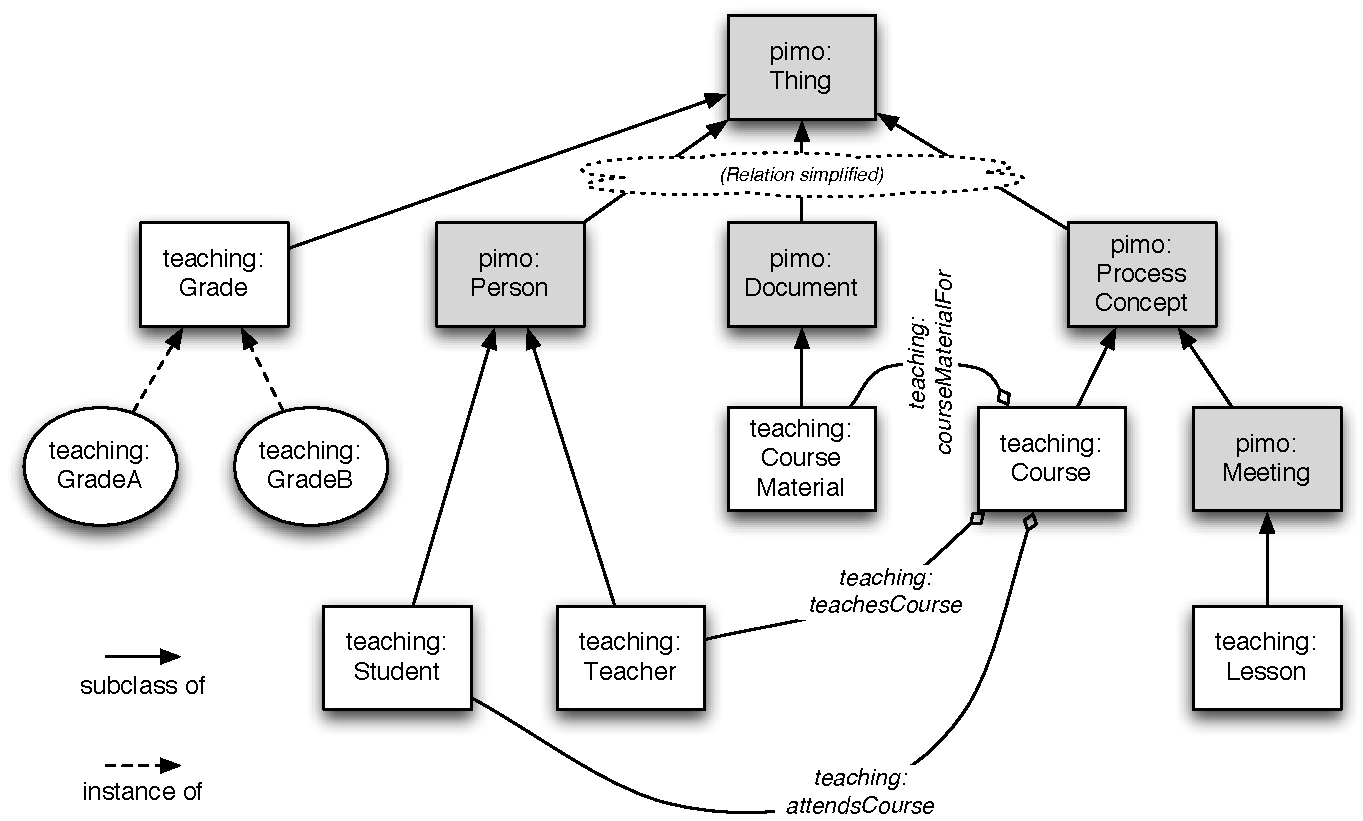
\includegraphics[width=\linewidth]{images/PIMOextensionExample-Teaching}
    \caption{Extending PIMO with new classes, properties and instances for the domain of teaching}
    \label{fig:extensionExampleTeaching}
  \end{center}
\end{figure}

\begin{figure}
  \begin{center}
	\begin{verbatim}
# new classes:
   teaching:Grade a rdfs:Class;
      rdfs:subClassOf pimo:Thing.

   teaching:Student a rdfs:Class;
      rdfs:subClassOf pimo:Person.

   teaching:Teacher a rdfs:Class;
      rdfs:subClassOf pimo:Person.

   teaching:CourseMaterial a rdfs:Class;
      rdfs:subClassOf pimo:Document.

   teaching:Course a rdfs:Class;
      rdfs:subClassOf pimo:ProcessConcept.

   teaching:Lesson a rdfs:Class;
      rdfs:subClassOf pimo:Meeting.

# new properties and their inverse:
   teaching:courseMaterialFor a rdf:Property;
      rdfs:subPropertyOf pimo:partOf;
      rdfs:domain teaching:CourseMaterial;
      rdfs:range teaching:Course;
      nrl:inverseProperty teaching:hasCourseMaterial.
   teaching:hasCourseMaterial;
      rdfs:subPropertyOf pimo:hasPart;
      rdfs:domain teaching:Course;
      rdfs:range teaching:CourseMaterial;
      nrl:inverseProperty teaching:courseMaterialFor.

   teaching:teachesCourse a rdf:Property;
      rdfs:subPropertyOf pimo:related;
      rdfs:domain teaching:Teacher;
      rdfs:range teaching:Course;
      nrl:inverseProperty teaching:taughtBy.
   teaching:taughtBy a rdf:Property;
      rdfs:subPropertyOf pimo:related;
      rdfs:domain teaching:Course;
      rdfs:range teaching:Teacher;
      nrl:inverseProperty teaching:teachesCourse.
      
   teaching:attendsCourse a rdf:Property;
      rdfs:subPropertyOf pimo:related;
      rdfs:domain teaching:Student;
      rdfs:range teaching:Course;
      nrl:inverseProperty teaching:attendeeStudent.
   teaching:attendeeStudent a rdf:Property;
      rdfs:subPropertyOf pimo:related;
      rdfs:domain teaching:Course;
      rdfs:range teaching:Student;
      nrl:inverseProperty teaching:attendsCourse.

# new instances:
    teaching:GradeA a teaching:Grade;
      nao:prefLabel "A".

    teaching:GradeB a teaching:Grade;
      nao:prefLabel "B".

    ...
	\end{verbatim}
    \caption{Extending PIMO with new classes, properties and instances for the domain of teaching --- N3 code}
	\label{fig:extensionExampleTeachingN3}
\end{center}
\end{figure}

\paragraph{Inheritance} % (fold)
\label{par:inheritance}

Sub-classing any class from PIMO (whether it be existing classes from PIMO-upper or classes that have been added later) also means that the new sub-class can be used with the same properties that have been defined with its superclass. Remember that NRL has a closed world assumption, and not an open world assumption, as RDFS traditionally has. In NRL\footnote{\url{http://www.semanticdesktop.org/ontologies/nrl/}}, ontologies can be used to validate statements.
%\note{reference to NRL spec --- 05.01.08, done}
E.g., if the property \texttt{name(pimo:Person, String)} has been defined, and if we define our new class \texttt{teaching:Student} to be a sub-class of \texttt{pimo:Person}, then this will allow us to use \texttt{name} with instances of \texttt{Student} as well - an NRL validator will permit this, because all instances of \texttt{Student} are also instances of \texttt{Person}. An example of this is shown in Fig.~\ref{fig:propertyInheritance}: this concept is very similar to the idea of inheritance in object-orientation, even though strictly speaking it is not the same.

% paragraph inheritance (end)

\begin{figure}
  \begin{center}
	\begin{verbatim}
		
   pimo:name a rdf:Property;
      rdfs:Domain pimo:Person;
      rdfs:Domain rdfs:Literal.
		
   teaching:Student a rdfs:Class;
      rdfs:subClassOf pimo:Person.

   knud a teaching:Student;
      pimo:name "Knud M�ller".

	\end{verbatim}
    \caption{``Inheritance'' of properties}
	\label{fig:propertyInheritance}
\end{center}
\end{figure}

% subsection subclassing_pimo_upper (end)

\subsection{Markup for the new ontology}
\label{sec:extendingontologymarkup}
The teaching ontology still needs to be defined as proper NRL ontology
to be usable with PIMO. The ontology \textbf{must} to be identified via its URI
and the author of the ontology can be added
as \texttt{nao:creator}.

\begin{verbatim}
teaching:TeachingOntology a nrl:Ontology;
 nao:creator teaching:TeachingOntologyCreator.

teaching:TeachingOntologyCreator a nao:Party;
 rdfs:label "Knud M�ller".

\end{verbatim}

\subsection{Information Elements} % (fold)
\label{sub:information_elements}

An important feature of the NEPOMUK ontology architecture is the fact that it is divided into two tiers: the PIMO tier and the Native Structures tier, as defined in the NEPOMUK Information Element Ontology (NIE)\footnote{\url{http://www.semanticdesktop.org/ontologies/nie/}} and its sub-ontologies, such as the NEPOMUK File Ontology (NFO)\footnote{\url{http://www.semanticdesktop.org/ontologies/nfo/}}.
%\note{reference to NIE spec --- 05.01.08, done}
While the former covers the internal mental model of a user or an organization (people, events, projects, etc.), the latter covers the physical representations of data (address book entries, calendar entries, files, etc.). Obviously, there are numerous connections between the tiers: people are represented by address book entries, events appear in the calendar, projects have files associated to them.

Whenever classes that are introduced to PIMO have a physical representation on the user's desktop, a connection to NIE must be modeled as well. Consider the example of the teaching ontology above: Such an ontology will contain classes for Things like exams and essays. Those classes belong to the PIMO tier. Their representation within the computer --- e.g., as text files --- belongs to the native structures tier. Or, in a more complex case, the new ontology could very well come with a specialized application, such as a Training Course Manager, where users can assign attendees to trainings, etc. In this case, people and courses (PIMO tier) would be represented by the application as application-specific data structures or information elements (native structures tier). In both cases a link from the new PIMO classes to the information elements represented with NIE is required to fully exploit the possibilities of the semantic desktop.

% subsection information_elements (end)

%\note{Knud, 05.01.08: I decided to drop the Author class in the BibTeX example. Authors should really just be pimo:Persons, not a subclass thereof.
%Leo, 8/1: OK, DONE}

As a second example, we can consider an ontology for scientific publications. This ontology (which would probably be based on Bib\TeX), would come with classes such as \texttt{Article} or \texttt{Book} and relations between them like \texttt{bookContainsArticle} or \texttt{hasAuthor}. For the integration into PIMO, \texttt{Article} would most likely become a sub-class of \texttt{pimo:Document}. 
Documents have	two types: one which anchors them in the PIMO tier, and one which anchors them in the native structures tier.
The \texttt{pimo:LogicalMediaType} (and its sub-classes, e.g., \texttt{pimo:Document}) captures how a document is interpreted by the user and belongs to the PIMO tier. Logical media types can be contracts, invoices, assignments, invitations, law texts, etc. 
The other type, which is the \texttt{nfo:Document} type, captures how the system interprets the document, and belongs to the native structures tier.
This is the physical document type as modeled by NIE.
Instances of a logical media type can have various representations in the native structures tier: 
for example, a text interpreted as an invoice by the user can either be an \texttt{nfo:PlainTextDocument} or an \texttt{nfo:PaginatedTextDocument}. 
Vice-versa, one physical type can be used to represent both an invitation or an invoice, which are different logical media types.
Keeping this this separation of content and representation in mind, one can model concrete documents having two types, one on each tier.

\begin{figure}
  \begin{center}
\begin{verbatim}
bibtex:Article a rdfs:Class;
 # PIMO tier: interpreted by the user as nie:Document
 rdfs:subClassOf pimo:Document; 
 # native structures tier: interpreted by the system as nfo:TextDocument
 rdfs:subClassOf nfo:TextDocument. 

bibtex:hasAuthor a rdf:Property;
 rdfs:subPropertyOf pimo:related;
 rdfs:subPropertyOf nfo:creator;
 rdfs:domain bibtex:Article;
 rdfs:range pimo:Person.
 
bibtex:hasLCCN a rdf:Property;
 rdfs:subPropertyOf nao:identifier; \# add an identifier
 rdfs:domain bibtex:Article.
\end{verbatim}
    \caption{A Bib\TeX-based PIMO extension for scientific publications}
	\label{fig:bibtexExample}
\end{center}
\end{figure}
%bibtex:Author a rdfs:Class; 
% # this adds properties like Name
% rdfs:subClassOf pimo:Person. 

\subsection{Extension by Sub-classing from External Classes} % (fold)
\label{sub:extension_by_subclassing_from_external_classes}

\textbf{Another possibility is extending existing PIMO-upper classes by sub-classing them from external classes.} \emph{This is discouraged}. For example, if the class \texttt{pimo:Person} was defined a sub-class of \texttt{nco:PersonContact} and \texttt{pimo:Organization} a sub-class of \texttt{nco:OrganizationContact}, all instances of these classes would automatically be inferred to be \texttt{pimo:Thing}s. However, those instances would probably not have some of the properties required by the \texttt{Thing} defined, which would render the imported data invalid. 
Similarly, when a mapped class X has cardinality restrictions on its properties (such as required properties), adding X as new superclass to an existing PIMO class can render the instances of the PIMO class invalid. 

% subsection extension_by_subclassing_from_external_classes (end)

\subsection{Summary} % (fold)
\label{sub:summary}

The very condensed summary to extending PIMO and mapping frome existing ontologies to PIMO is the following:

\begin{itemize}
  \item Make classes sub-classes of PIMO-upper classes.
  \item Make properties sub-properties of PIMO-upper properties.
	\item Relations: Links between Things have to be browseable, properties should have inverse relations defined (see \cite{rohmer2005})
	\item Extensibility: Users are free to add new relation types and new classes (see \cite{rohmer2005})
\end{itemize}

% subsection summary (end)

\section{Importing Domain Ontologies into a User's PIMO}
\label{sec:importingontologies}
%\note{Written by Leo, but Knud: feel free to mash it up}
Once modeled, the new domain ontology such as the teaching ontology in the previous examples can be made available publicly for others, for example by publishing it on the Web. A good reference for doing this is \emph{Best Practice Recipes for Publishing RDF Vocabularies}~\cite{SWBPVocabularyRecipes}.

% adressing
Semantically, an imported ontology is captured using a \texttt{nrl:imports} statement.
When a user imports a domain ontology, this statement \textbf{should} be added.

{\small
\begin{verbatim}
claudia:Pimo nrl:imports teaching:TeachingOntology.
\end{verbatim}
}

%Importing the ontology to a Sematic Desktop or other Personal Information Management system can then be done by downloading the ontology file and storing it into the RDF store where the PIMO of the user is kept.
% Stuff like downloading is outside the scope of PIMO and really has no place in the PIMO specification
Once the user of a Semantic Desktop system imports an external PIMO into their own desktop, all new classes (which are sub-classes of \texttt{pimo:Thing}) \textbf{should} become available to them as if they had created those classes themselves.
Instances, on the other hand, are not automatically available.
As said in the introduction, the scope of a PIMO for an individual user is to model data that is within their own attention and needed for knowledge work or private use.
However, when importing external ontologies or knowledge bases, not all instances may be of interest to the user. As with imported information elements, a separate Thing is created to represent the imported resource within the PIMO of the user and connected to the imported instance using \texttt{pimo:hasOtherRepresentation}\footnote{An alternative would be to treat all Things present in the RDF data available of the user as if they were created by the user, imported or not. This has the drawback that it allows to represent the same real-world entity twice, first in the imported domain ontology and second in the user's own PIMO.}.
Before creating a new Thing for an imported instance, the PIMO of the user has to be checked if the entity is already represented as a Thing, as indicated above in Section~\ref{sec:creatingthingalgorithm}.
Once represented as a Thing in the user's PIMO, it is possible to assign a personal identifier to it, annotate it, and use it. 

Implementations \textbf{must} automate the importing process. The user should be able to interact with imported Things as if they were created by themselves. 

\begin{comment}
LEO: THIS COMMENTED OUT NOW, ITS TOO SCIENTIFIC.
\section{Design Rationale}
\label{sec:designrationale}
In this section the design rationale behind \pimo and the sources which influenced us are described. 
% COPIED FROM SauermannElstDengel2007
%The motivation for creating the PIMO is to find a language to name the terms
%that are relevant to a knowledge worker and to have ways to express facts about
%these terms. Once this language is defined and formalized in the ontological
%description of the PIMO, it can be used to translate existing resources, and to
%express information about them. The PIMO is a user-centric view on existing
%documents, domain ontologies, and web data sources.
%
%While the organization asks for universally applicable and standardized
%persistent structures, processes, and work organizations to achieve and
%maintain universally accessible information archives, the individual knowledge
%worker requests individualized structures and flexibility in processes and work
%organization in order to reach optimal support for the individual activities.
%
The vision behind this work is that a \emph{Personal Information Model} reflects and captures a user's
personal knowledge, \eg about people and their roles, about organizations, processes,
things, and so forth, by \emph{providing the vocabulary} (concepts and their relationships)
required for expressing it as well as concrete instances. In other words, the domain of a
\pimo is meant to be ``all Things and native resources that are in the attention of the
user when doing knowledge work''.
\note{Knud, 07.01.08: Probably quickly explain what native structures are?}
Though ``native'' information models and structures are
widely used, there is still much potential
for a more effective and efficient exploitation of the underlying knowledge. We think that,
compared to the cognitive representations humans build, there are mainly two shortcomings
in native structures:
\begin{itemize}
  \item \emph{Richness of models}: Current state of cognitive psychology
  assumes that humans build very rich models, encoding not
  only detailed factual aspects, but also episodic and situational
  information. Native structures are mostly taxonomy- or
  keyword-oriented.
  \item \emph{Coherence of models}: Though nowadays (business)
  life is very fragmented humans tend to interpret situations as a
  coherent whole and have representations of concepts that are comprehensive
  across contexts. Native structures, on the other hand, often
  reflect the fragmentation of multiple contexts. They tend to be
  redundant (i.e., the same concepts at multiple places in
  multiple native structures). Frequently, inconsistencies are the
  consequence.
\end{itemize}

The \pimo shall mitigate the shortcomings of native structures by providing a
\emph{comprehensive model} on a \emph{sound formal basis}.

% next snip
%When building concrete \pimos, we now have the
%problem of two, potentially conflicting demands: On the one hand, we want to give the user
%the opportunity to span his information space largely in the way \emph{he} wants. The
%\pimo should model \emph{his} mental models. In consequence, we cannot prescribe much of
%this structure. On the other hand, ``empty'' systems often suffer from the cold
%start problem, being not accepted by user when not already equipped with some initial content.
%Using a multi-layer approach (see also \cite{Sauermann+2006d}), we try to find a balance through providing 
%the presentational basis as given, which users \emph{can} incorporate or extend:
%by a layered approach to \pimos : The representational basis
%as well as the basic dimensions of a \pimo are pre-given, but flexible enough for simple as
%well as more advanced modeling. Lower levels are meant as a proposition; when establishing
%an individual \pimo, users \emph{can} incorporate them into their model if they find them
%adequate and useful, but they don't have to. In the following, we briefly sketch the
%proposed \pimo layers:

% NOTE: THIS IS BAD, PIMO-MID IS a FORBIDDEN WORD and therefore replaced with XXXXXXX
%\subsection{PIMO-Basic, PIMO-Upper, PIMO-XXXXXXX and Domain Ontologies}
%Apart from the native structures, the mental models are represented using a multi-layer
%approach. These layers are:
%\begin{itemize}
%  \item PIMO-Basic: defines the basic language constructs. The class
%  pimo-basic:Thing represents a super-class of other classes.
%  \item PIMO-Upper: A domain-independent ontology defining abstract sub-classes of
%  Thing. Such abstract classes are PersonConcept, OrganizationalConcept,
%  LocationConcept, Document, etc.
%  \item PIMO-XXXXXXX: More concrete sub-classes of upper-classes. The
%  mid-level ontology serves to integrate various domain ontologies and provides
%  classes for Person, Project, Company, etc.
%  \item Domain ontologies: A set of domain ontologies where each describes a
%  concrete domain of interest of the user. The user's company and its
%  organizational structure may be such a domain, or a shared public ontology.
%  Classes are refinements of PIMO-XXXXXXX and PIMO-Upper, allowing an integration
%  of various domain ontologies via the upper layers.
%  \item PIMO-User: the extensions of above models created by an individual for
%  personal use. Classes, properties and Things are created by the user.
%\end{itemize}

% END OF SauermannElstDengel2007
\end{comment}


\section{Practical Directions on Using PIMO}
In this section, a few issues that will arise in actual PIMO usage are discussed. For each of these issues, we will suggest a recommended way of handling them. Even though those things are not strictly speaking part of the ontology, they are part of the standard defining how to use the PIMO ontology in applications.
Implementers \textbf{should} conform to these directions.

\subsection{Creating Things}
\label{sec:creatingthingalgorithm}
New PIMO Things can be created freely, but usually the creation of a Thing is rooted in the existence of an information element.
An algorithm to create new Things based on information elements \textbf{should} follow these steps:

\paragraph{Start} The software agent encounters a resource with URI $X$ and wants to verify if the user already has knowledge about \textbf{$X$}. 
\paragraph{Check GroundingOccurrence} Query the user-PIMO for:
\begin{verbatim}
SELECT ?thing WHERE {?thing pimo:groundingOccurrence ?X.}
\end{verbatim}
When a Thing is found, finished.
\paragraph{Check occurrences} Repeat the last step to search if $X$ is an occurrence of a Thing.
\paragraph{Check identifiers} Validate if the InformationElement has an identifier or a referencing occurrence that is also used on an existing Thing. The information element is called an \textbf{occurrence} of a Thing when it shares the same identifiers. The correct query is:
\begin{verbatim}
SELECT ?thing  
WHERE {
?thing ?p ?o. 
?X ?p ?o. 
?p rdfs:subPropertyOf nao:identifier.
} UNION {
?thing ?p ?o. 
?X ?p ?o. 
?p rdfs:subPropertyOf pimo:referencingOccurrence.
}
\end{verbatim}
When a Thing is found, finished.
\paragraph{Create a new Thing}
When the last step did not return an existing Thing, this can be an indicator that element $X$ is new to the user and should be modeled with a new Thing. 
Mint a new URI and add the identity values from the InformationElement. 

In the following SPARQL query example, we assume that Claudia's System has just encountered a new calendar event $X$ and represents it using the new minted URI $claudia:Event42$. 
{\small
\begin{verbatim}
CONSTRUCT { 
<claudia:Event42> rdf:type pimo:Thing.
<claudia:Event42> ?i ?io.
<claudia:Event42> nao:prefLabel ?title.
<claudia:Event42> rdf:type  ?type.
<claudia:Event42> rdf:type  ?pimotype.
<claudia:Event42> pimo:groundingOccurrence ?X.
<claudia:Event42> nao:created ``2007-06-30T18:11:00Z''.
<claudia:Event42> pimo:isDefinedBy claudia:PIMO.
} WHERE {
OPTIONAL (?X ?i ?io. ?i rdfs:subPropertyOf nao:identifier.).
OPTIONAL (?X nie:title ?title).
OPTIONAL (?X rdf:type  ?type).
OPTIONAL (?X rdf:type  ?type. ?pimotype rdfs:subClassOf ?type.
 ?pimotype rdfs:subClassOf pimo:Thing).
}
\end{verbatim}
}
The different parts of this query are:
\begin{itemize}
	\item all identifiers are copied (?i, ?io)
	\item the title is copied for readability and to use it for tagging (?title)
	\item the original type(s) are copied (?type)
	\item find possible PIMO:Thing classes that can be used for this type (?pimotype)
	\item the groundingOccurrence relation is added
	\item the created timestamp is set to the current date
	\item the isDefinedBy relation is set
\end{itemize}
Finding a suitable class to represent the resource
in the PIMO depends on a mapping of information element classes to PIMO classes
and can be realized in different ways, see Section~\ref{sec:classofthing}.

\subsection{Changing the Type of a Thing}
\note{Knud, 06.01.08: Can we change "Thing" into "Instance" (also below)? To me, "thing" sounds much too ambiguous.
\emph{Leo, 8/1:}I would stick to \texttt{Thing} as a word used before}
Changing the type of an instance can lead to invalid statements in the knowledge base. E.g., this can happen when the instance in question is involved in statements using a property with a specific domain and range, and the new type is not compatible to those.
As this would render the model invalid, this situation must be avoided in applications interacting with PIMO data.
A user interface should remind the user of possible problems and should suggest solutions. 

\note{Knud, 06.01.08: Is it even possible that domain and range are not set in NRL? If not, maybe remove this paragraph. 
\emph{Leo, 8/1:} NRL does not require it} A different approach is ontology-by-examples where the main principles is that ``the user is always right'' and domain/range values are not explicitly set but implied by previous usage. 
User interfaces may support this behavior by setting the domain and range to \texttt{pimo:Thing} and suggest properties suitable for class by analysing previous usage of the property.

\subsection{Deleting a Thing}
We can say that, in RDF, instances do not exist independently, but only as part of statements. Thus, ``deleting an instance'' really means deleting all statements in which this instance is involved (as subject or object).
%Note, that also \texttt{pimo:creationSupportedBy} links will be deleted by this, which may result that an algorithm soon creates the instance again (if the user somewhere configured to created instances automatically). See below in section Automatic Creation of Things from ResourceManifestations. 
%In this case, it may be better to use the \texttt{pimo:metaHidden} property to hide it.
\note{Knud, 06.01.08: this needs to be explained, otherwise it's incomprehensible.
\emph{Leo, 8/1:} actually, the groundingForDeletedThing is the needed Thing, I described it.}
If the instance has a grounding occurrence relation, a new \texttt{pimo:groundingForDeletedThing} relation should be created to record the deletion.
Data integration algorithms analysing resource to automatically create Things can then avoid re-creating the already deleted Thing.

\subsection{Deleting User-generated Classes and Properties}
Deleting a user-generated class is allowed but requires that instances are re-typed to the direct super-class of the deleted class. Also the domains and ranges of all properties defined with the class as domain or range need to be changed to the direct superclass. 
These changes are necessary to prevent the model from becoming invalid.
Classes defined in the pimo language cannot be deleted, only classes defined by the user can be deleted.

The direct super-class $S$ of the class $C$ is defined as the class where no other class $T$ exists where $C$ has superclass $T$ and $T$ has superclass $S$. If there are multiple $S$, all of them should be used as replacement when deleting a class.

%\note{Knud, 06.01.08: Saying that something is ``forbidden'' sounds really strange. Also, why not just say: \emph{If user-generated properties are deleted, this requires all statements in which those properties are involved to be deleted as well, in order to prevent the model to become invalid. Alternativaly, all occurrences of the property could be replaced by its super-property.}
%\emph{Leo, 8/1:OK}} 
If user-generated properties are deleted, this requires all statements in which those properties are involved to be deleted as well, in order to prevent the model to become invalid. 
Alternatively, all occurrences of the property could be replaced by its super-property.
%This would be analogous to how classes are handled.} Deleting a user-generated property that was used as predicate in statements is forbidden, as it is not clear what the semantics of the statements would be nor what property should be used as replacement in the statements. User-generated properties can be deleted when all statements using them are deleted a priori.



\subsection{Merging Duplicates}
\label{sec:mergeduplicates}
\emph{Duplicates} are two Things that represent the same real-world entity within a user's PIMO. As we apply the unique name assumption (two Things with different names are different), duplicates should be found and corrected. 
When duplicates are found, both (the ``duplicate'' and the ``original'') can be merged into one single instance.
In this process, RDF statements involving the duplicate are changed so that they now refer to the original.
In a local setup with one desktop and all data stored in a single database, this process is without information loss and causes no side-effects. As Semantic Web applications are in a distributed scenario, deleting a duplicate resource can cause dangling links in related databases and other side-effects. 
\note{Knud, 06.01.08: The idea of dangling links here is a bit misleading here. It implies that the Thing the link refers to is somehow \emph{gone}. However, the Thing was never really there --- there are always only statements about Things.} 
\note{Leo: no, its ok. Deleting/merging Things may cause these problems the suggested
hasDeprecatedRepresentation fixes it like a 301 ``moved permanently''} 

For this, the \texttt{pimo:hasDeprecatedRepresentation} property \textbf{should} be used to relate the original with the (now deleted) duplicate. Note that the range of this property is not defined, as all data about the duplicate resource (including the type) is deleted.

When merging two duplicate resource $A$ and $B$ into one resource $C$, a few practical guidelines can reduce side-effects:
\begin{itemize}
	\item The URI of $C$ is either $A$ or $B$, the older resource (as defined by \texttt{nao:creationDate}, see Section~\ref{sec:changedates}) is to be preferred as it has a higher chance of being used.
	\item The classes of $C$ are the union of the classes of $A$ and $B$.
	\item All statements about $A$ and $B$ are merged to $C$.
\end{itemize}

\subsection{Unification of multiple Information Elements into one Thing}
\label{sec:unification}
In comparison to merging duplicate Things, \emph{unification} is the process when multiple information elements representing the same real-world entity are mapped to one \texttt{pimo:Thing} instance.

In PIMO, multiple information elements representing one real-world entity are mapped to exactly one \texttt{pimo:Thing} instance using the \texttt{pimo:groundingOccurrence} and \texttt{pimo:occurrence} relations. 
Algorithms or user interfaces implementing unification must consider the identifying properties of a Thing (see Section~\ref{sec:identification}) when searching for possible Things to representing information elements.
%If algorithms don't find an existing Thing to represent and information element, they should create a new instance. See Section~\ref{sec:classofthing} about suitable PIMO classes to represent information elements.

Four default \textbf{NRL Views} and \textbf{NRL ViewSpecifications} are defined for different levels of inference. Each creates a named graph that contains the instance data and the inferred statements.

\begin{description}
	\item[\texttt{pimo:InferOccurrences}] a view that infers occurrences based on \texttt{nie:identifiers} and pimo:referencingOccurrence annotations.
	\item[\texttt{pimo:GroundingClosure}] a view that adds statements about the grounding Occurrences and \texttt{hasOtherRepresentation} to a Thing.
	\item[\texttt{pimo:OccurrenceClosure}] a view that adds statements about all occurrences to a Thing.
	\item[\texttt{pimo:FullPimoView}] a supergraph of all above.
\end{description}

By providing these graphs, we let the user and software agent decide if the full closure is needed at all times. When no closure is needed, the plain NRL data graphs can be used as-is.
To answer complex queries like ``Which e-mails were sent to me by attendees of meetings that I have today'', the full closure is a good choice.

The ability to superimpose data using inference limits the data needed in a PIMO to a necessary minimum: only the identification properties are mandatory, the occurrence and the hasOtherRepresentation properties superimpose existing data. 

\begin{verbatim}
claudia:DirkHagemann a pimo:Person;
 pimo:occurrence <imap://claudia@example.com/INBOX/1#from>;
 pimo:groundingOccurrence <file://home/claudia/dirk.vcf#dirk>.
\end{verbatim}


Using the guiding example, an integrated view of Claudia on Paul is the following, assuming full closure:
{\small
\begin{verbatim}
# The canonical Dirk
claudia:DirkHagemann a pimo:Person;
# the second type is also inferred
 a nco:PersonContact;
 pimo:isDefinedBy claudia:PIMO;
 nao:prefLabel 'Dirk Hagemann';
 nao:identifier "dirk@example.com";
 pimo:occurrence <imap://claudia@example.com/INBOX/1#from>;
 pimo:groundingOccurrence <file://home/claudia/dirk.vcf#dirk>;
 pimo:referencingOccurrence <http://www.example.com/people/DirkHagemann>;
 pimo:hasOtherRepresentation <http://id.example.com/person/1650>;
# the inferred facts
 nco:hasEmailAddress <mailto:dirk@example.com>;
 nco:nameFamily "Hagemann";
 nco:nameGiven "Dirk";
 nco:photo <http://www.example.com/people/dirk/photo.jpg>.
 
# E-mail, now pointing to the canonical Dirk
<imap://claudia@example.com/INBOX/1> a nmo:Mail;
 nmo:from claudia:DirkHagemann.
\end{verbatim}
}

%From the perspective of the user, facts stated about grounding occurrences are correct (they have been taken from existing data managed by the user); as are hasOtherRepresentation 
%(they are from formal ontologies imported and accepted by the user). If this is not the case, the incorrect statements must not be integrated, which is interesting but out of the scope of PIMO for now.
%As a result of the unification process, one Thing points to multiple information elements. This is also reflected in the previous examples, such as this:

\subsection{Tagging and Annotating Files}
\label{sec:taggingfiles}
Conceptually, once an Information Element (a file, an e-mail, a webpage, an address book entry, etc.) 
is in the attention of the user
and is read or annotated, it is also a Thing in the mental model of the user.
A core idea of the Semantic Desktop is to use other Things as dimensions to annotate files and retrieve them later, as described in~\cite{Dengel2006}.

Lets assume the file \texttt{/home/claudia/doc/tripplan.pdf} is to be tagged with the  tag ``Belfast Meeting Package''.

A representation of the file is already extracted by the semantic desktop data wrapper system
(or any other content management system):

\begin{verbatim}
<file://home/claudia/doc/tripplan.pdf> a nie:TextDocument;
 nie:language "en";
 nie:title "Belfast Bus Timetable".
\end{verbatim}

Additionally, the city of Belfast and the Belfast meeting package already exist in the model, as well as a \texttt{MeetingPackage} class (which was either created by Claudia, or came as part of a shared domain/group ontology):
\begin{verbatim}
claudia:BelfastMeetingPackage a claudia:MeetingPackage, pimo:Tag;
 pimo:tagLabel "Belfast Meeting Package";
 pimo:isDefinedBy claudia:PIMO.
\end{verbatim}

To add a simple tag, the file is now represented as a Thing (\textit{thingified}) and
the tagging relation set.

\begin{verbatim}
claudia:BelfastBusTimetable a pimo:Document;
  nao:prefLabel "Belfast Bus Timetable";
  pimo:isDefinedBy claudia:PIMO;
  pimo:groundingOccurrence <file://home/claudia/doc/tripplan.pdf>;
  nao:hasTag claudia:BelfastMeetingPackage.
\end{verbatim}

The interested reader may now ask, ``but why create a new Thing and
not just add the nao:hasTag relation directly to the file?''
The reason to \textit{thingify} the file is twofold:
first, it is possible to assign a new class to the file, for example
creating the class \texttt{claudia:BusTimetable}. 
Second, the same timetable may be available in different data objects,
if it is stored in an e-mail attachment, a web resource,
or a local file --- it is always the same document.
A tag added to one occurrence of the file is also valid for other occurrences. Also refer to Sections~\ref{sec:pimoVSnie},\ref{sub:information_elements}.

Given Claudia finds the same timetable on a website, the system
can link the two based on \texttt{nie:identifiers} (which should be globally unique 
identifiers for information elements, independent of the data object
they are stored in). This example shows this case (with copied identifiers):

\begin{verbatim}
# the file on the harddisk
<file://home/claudia/doc/tripplan.pdf> a nie:TextDocument;
 nie:language "en";
 nie:title "Belfast Bus Timetable";
 # this isbn is fictional
 nie:identifier "ISBN:12123-123123".
 
<http://www.buseireann.ie/timetables/belfast.pdf>
 a nie:TextDocument;
 nie:title "Belfast Bus Timetable";
 # this isbn is fictional
 nie:identifier "ISBN:12123-123123".
 
claudia:BelfastBusTimetable a pimo:Document;
  pimo:isDefinedBy claudia:PIMO;
  pimo:groundingOccurrence <file://home/claudia/doc/tripplan.pdf>;
  pimo:occurrence <http://www.buseireann.ie/timetables/belfast.pdf>;
  nie:identifier "ISBN:12123-123123";
  pimo:hasTag claudia:BelfastMeetingPackage.
\end{verbatim}
The tag assigned to the bus time table is now valid,
independent of the data object.

Using the generic tag relation \textbf{pimo:hasTag} is 
an easy-to-use entry point for users that don't need
formal semantic relations.

Using the property \emph{nao:hasTag} is not sufficient
to be PIMO conformant, implementers \textbf{must} use
the \emph{pimo:hasTag} relation for desktop tagging.
The \emph{nao:hasTag} property and \emph{nao:Tag} class are reserved for data of information elements that are imported into a PIMO.

\textbf{Example}: The Belfast Bus Timetable has the topic Belfast,
which is not just a Tag but says more about the relation between the 
timetable and the city. The \textbf{has Tag} relation can be used for this:
\begin{verbatim}
claudia:BelfastBusTimetable a pimo:Document;
 pimo:hasTag claudia:Belfast.
\end{verbatim}

\textbf{Example}: The relation between Claudia and the 
BelfastMeetingPackage can be expressed using ``has tag'' but 
may also be represented with a relation saying more about
the semantics: Claudia is ``attending this meeting''. 
Assuming that the MeetingPackage is a sub-class of meeting,
this could be expressed like:
\begin{verbatim}
claudia:BelfastMeetingPackage a meeting:MeetingPackage.

# instead of nao:hasTag, a semantic relation is used
claudia:Claudia pimo:attendee claudia:BelfastMeetingPackage.
\end{verbatim}

\subsection{Geo-locating Things}
Things can be geo-located, meaning that their geographical location is set using latitude, longitude and altitude information in the WGS84 geodetic reference datum.
In PIMO, the location is a separate entity of type \texttt{Location}, and other items can then be geo-located there. The relation \texttt{pimo:hasLocation} is used for this, \texttt{pimo:isLocationOf} is the inverse.
There is an abstract marker class for locatable Things: pimo:Locatable.
Social events, organizations, persons, and physical objects are locatable. 

To add a location to a meeting, this data is added, for your reference the location is also given:
\begin{verbatim}
claudia:InitialMeetinginBelfast a pimo:Meeting;
  nao:prefLabel "Initial Meeting in Belfast";
  pimo:hasLocation claudia:Belfast.
  
claudia:Belfast a pimo:City;
  nao:prefLabel "Belfast";
  geo:lat "54.5833333";
  geo:long "-5.9333333".
\end{verbatim}

Usually, locations should be reused to locate multiple Things,
but new locations can of course be generated anytime.

PIMO defines a number of general-purpose classes for countries, states, cities, buildings, and rooms, which we consider independent of culture and domain. Domain-specific ontologies can specify those classes further.
In the rare case when the type of location cannot be specified with any of the existing classes, the superclass \texttt{pimo:Location} can be used.
In some application scenarios (such as geo-locating a large amount of photos or measurement values), many locations would be needed.
To simplify annotation and remove clutter, specialized vocabularies may
then be used, as for example done in the NEXIF vocabulary for photos.

\subsection{Defining what is in the PIMO and what is not: NRL Graphs and \texttt{definedBy}}
\label{sec:nrlgraphs}
The facts (i.e., the statements) used to describe Things should be kept in named graphs according to the NRL standard. This allows to express metadata about the facts, such as to which
PIMO the Things belong (see Sect.~\ref{sub:connectingThingsToPimo}) or when individual triples were changed (see Sect.~\ref{sec:changedates}) and by whom.
Another important feature is to find which Things are in the user's PIMO and 
which not. In a shared environment, users may often import group-level ontologies that contain 
Things modeled by others. Considering this, it is important to keep up-to-date as to who said what, or, in other words, to detect if a Thing was modeled by the user or not.

All data expressed about Things can be kept in NRL graphs. 
The minimal metadata is:
\begin{itemize}
	\item The type of the graph is \texttt{nrl:KnowledgeBase}, as it can contain both instances and ontology constructs (see the NRL specification for more details).
	\item The graph is imported into the user's PIMO.
\end{itemize}
Additional metadata such as \texttt{nao:created} can be added.
These facts can be expressed in a separate metadata graph.
An example of how this looks like in code using Trig Notation\footnote{\url{http://sites.wiwiss.fu-berlin.de/suhl/bizer/TriG/}}:

\begin{verbatim}
# The instance data
claudia:graph1 {
  claudia:DirkHagemann a pimo:Person;
    nao:prefLabel 'Dirk Hagemann'.
}
# The metadata
claudia:graph1_metadata {
  claudia:graph1 a nrl:KnowledgeBase;
  claudia:PIMO nrl:imports claudia:graph1.
}
\end{verbatim}


\textbf{As not all implementers can or want to use NRL graphs to keep track of the boundaries of a PIMO, 
\texttt{pimo:isDefinedBy} must be used} to connect classes, properties, and instances to the PIMO that defines them\footnote{Separation based on the namespace was considered by some to be enough, but is not (as stores use fulltext comparison to handle namespaces, namespaces as such don't exist in RDF but only in XML).}.

To support both ways of detecting the boundaries of a user-PIMO, 
implementations \textbf{may} add the NRL metadata in addition to the \texttt{pimo:isDefinedBy} 
statements to the generated data. 
Resulting in:

\begin{verbatim}
# The instance data
claudia:graph1 {
  claudia:DirkHagemann a pimo:Person;
    pimo:isDefinedBy claudia:PIMO.
    nao:prefLabel 'Dirk Hagemann'.
}
# The metadata
claudia:graph1_metadata {
  claudia:graph1 a nrl:KnowledgeBase;
  claudia:PIMO nrl:imports claudia:graph1.
}\end{verbatim}

%This may produce legal but not valid NRL data, as explained in the NRL specification, Section 2.3.4
%\footnote{\url{http://www.semanticdesktop.org/ontologies/nrl/\#mozTocId220340}}.
%\note{Knud, 06.01.08: What does \emph{legal but not valid} mean?
%\emph{Leo, 8/1:}added link to NRL. DONE}

%\subsection{Annotating Websites}
% LEO: I cut that section, when we already have files, we don't need websites anymore.

%\subsection{Annotating an Event with NIE and PIMO}
% LEO: I cut that section, when we already have files, we don't need Event anymore.

\begin{comment}
\subsection{Annotating Resources without Creating New Things}
\label{sec:annotatingexternalresources}
\note{Knud, 06.01.08: To be honest, I find this section a bit esoteric (and I also admit I probably don't fully understand it). Do we really need this in the PIMO-Spec? I feel like we should try to keep the spec concise and drop this (would be nice in a paper, but not here).}
The interested reader may have come to the conclusion, that the suggested
way of handling annotation in PIMO is complicated and cumbersome; based 
on the observation that to annotate a file, a new ``Thing'' resource
has to be created. Creating a Thing requires minting a new URI, describing
it and linking it to the annotated resource using the \texttt{pimo:groundingOccurrence}
relation.

There are two reasons for this approach:
\begin{itemize}
	\item From a philosophical point of view, the resource can exist without the user's observation of it.
	The user annotates what perception and interpretation they have of the resource,
	a personal perspective. To represent it, the resource is ``thingified'', a new URI is minted,
	to represent that the ``user views the resource''.
	\item Technically, a newly minted URI inside the user's namespace has some qualities that
	make it a good RDF URI: it is retrievable, it does not change, it is unique.
\end{itemize}

But this also implies, that once a system satisfies both reasons, no new URI has to be minted.
A Semantic Web system to handle resources could fulfil these requirements:
\begin{itemize}
	\item Allow users to express their personal view on resources in a way that 
	represents ``this user has that view on resource X''. A possible technical 
	realization of this requirement is to use graph-metadata to annotate
	which triples are created by which user. The NRL specification allows this.
	\item URIs of resources have to be \textbf{retrievable}. Today, only a few web-applications
	hosting URIs fulfil all requirements of the Technical Architecture Group (TAG) 
	of the W3C towards Semantic Web URIs\footnote{See the decision taken to answer the
	http-range-14 issue at \url{http://lists.w3.org/Archives/Public/www-tag/2005Jun/0039.html}}.
	A human-friendly version of these requirements
	is written in \cite{Sauermann+2007a}. Simplified, servers must implement HTTP GET content 
	negotiation and return either RDF or HTML representations.
	\item An URI must not change. Some content management systems don't fulfill this,
	also none of the common file systems (when a file is moved, the URI changes)
	nor does it the IMAP URI scheme.
\end{itemize}

Simply put: the system storing resources to be annotated must be fully Semantic Web and NRL compliant.
Such resources could then be annotated directly, without creating Things and relating them to grounding occurrences.

\textbf{Example}: annotating a correct Semantic Web URI without creating a new URI for it.
\begin{verbatim}
# It is mandatory that the used URIs conform to the open linked data standards
@prefix claudia: <http://www.example.com/people/claudia#> .

# The annotation is about Tim Berners Lee,
# identified by a correct Semantic Web URI 
@prefix timblcard: <http://www.w3.org/People/Berners-Lee/card#>.


# A named graph containing the metadata about Graph1
claudia:Graph1Meta {
 claudia:Graph1 a nrl:KnowledgeBase;
   nao:creator claudia:Claudia.
 # The annotations are now part of her user-PIMO
 claudia:PIMO nrl:imports claudia:Graph1.
}
# This is the annotation by Claudia about Tim Berners Lee
claudia:Graph1 {
  # Claudia says: he is a Person
  timblcard:i a pimo:Person;
   # he is now also part of Claudia's personal view on the world,
   # this is valid within this graph
   pimo:isDefinedBy claudia:PIMO;
   # a tag is added
   nao:hasTag claudia:SemanticWeb.
}
\end{verbatim}
We would recommend to try this out experimentally, when you have access to 
a system that fulfils the requirements,
but not before. 
Without a proper NRL implementation, misleading information
could be inferred.
The PIMO framework is intended to work today,
therefore the pimo:groundingOccurrence relation and the minting of new
URIs is recommended. It is also compatible for
the next years, when Semantic Web and NRL compliant systems exist.
\end{comment}

\subsection{Using NAO and NIE Elements for Annotation}
\label{sec:usingnieinpimo}
Throughout this document, we have shown several uses of NAO and NIE elements
that can be applied to \texttt{pimo:Thing} instances. 

Semantically, we start from the assumption that a Thing modeled in PIMO is describing a concept from the real world.
On the other hand, the Thing itself can be viewed as a set of statements or triples stored in a computer system.
Thus, Things are resources and can be annotated with NAO.
Also, using PIMO closure as described in Sect.~{\ref{sec:integratingfacts},
facts of NIE elements can be inferred as facts of PIMO Things.
Thus, Things can also have a NIE class as type.

In Table~\ref{tab:SemanitcsOfNIEInPIMO} we give an overview of how the semantics of
the predicates may alter when interpreted within the PIMO.

The text ``\textbf{no change}'' means that the interpretation is unchanged, ``\textbf{not interpreted}'' means you should avoid interpreting this property in PIMO. You may notice that some properties are not interpreted because they have DataObjects or Strings as range, where PIMO has properties modeling the same semantics but using other \texttt{pimo:Thing}s as range, which is a more precise way of modeling because of the UNA.
``\textbf{Required}'' means that this property is required for all instances of \texttt{pimo:Thing}
and this can be validated using the rules from Section \ref{sec:validationrules}.
``\textbf{Recommended}'' means that you should use this property as if it is required, but it cannot be validated in NRL as property restrictions are only available in OWL.

The properties describing how information is stored (mime-type, bytesize, characterset) are obsolete for Things, as they describe a serialization.

\begin{table}[h!tbp]
	\centering
		\begin{tabular}{|l|p{0.7\textwidth}|}
		  \hline
			Term & Semantics\\
			\hline
			\texttt{nao:created} & \textbf{Recommended} When the RDF Resource representing this Thing was first created in the user's PIMO.\\
			\texttt{nao:identifier} & no change, used for identification and matching.\\
			\texttt{nao:lastModified} & \textbf{Recommended} When the Resource representing this Thing was last changed in the user's PIMO. Note that it can be different from the nie:contentLastModified property of a groundingOccurrence. When blending multiple groundingOccurrences into a Thing, the latest contentLastModified should be chosen.\\
			\texttt{nao:modified} & \textbf{Recommended}\\
			\texttt{nao:personalIdentifier} & \textbf{Not recommended}, \texttt{pimo:tagLabel} \textbf{must} be used.\\		
			\texttt{nao:prefLabel} & \textbf{Recommended}\\			
			\texttt{nie:characterSet} & \textbf{Not interpreted}, obsolete in RDF\\
			\texttt{nie:comment} & no change\\
			\texttt{nie:contentCreated} & \textbf{Not interpreted} \\
			\texttt{nie:contentLastModified} & \textbf{Not interpreted} \\
			\texttt{nie:contentSize} & \textbf{Not interpreted}, obsolete in RDF\\
			\texttt{nie:copyright} & no change, can be set by the user when sharing Things with others. See also nie:legal\\
			\texttt{nie:depends} & no change\\
			\texttt{nie:description} & no change\\
			\texttt{nie:disclaimer} & \textbf{not interpreted}\\
			\texttt{nie:generator} & no change, \texttt{pimo:Things} can be generated automatically by software or manipulated by user interfaces\\
			\texttt{nie:generatorOption} & no change\\
			\texttt{nie:hasPart} & \textbf{not interpreted}, \texttt{pimo:hasPart} should be used\\
			\texttt{nie:identifier} & no change\\
			\texttt{nie:isStoredIn} & \textbf{not interpreted}, \texttt{pimo:isDefinedBy} covers the storage.\\
			\texttt{nie:keyword} & \textbf{not interpreted}, should be modeled using hasTag and assigning the keyword as title of the topic.\\
			\texttt{nie:language} & no change\\
			\texttt{nie:legal} & no change, by default all legal properties scope all the statements having the same subject as the legal statement\\
			\texttt{nie:license} & no change\\
			\texttt{nie:licenseType} & no change\\
			\texttt{nie:links} & \textbf{not interpreted}, use pimo:related or pimo:hasTag\\
			\texttt{nie:mimeType} & \textbf{not interpreted}, obsolete in RDF\\
			\texttt{nie:plainTextContent} & no change\\
			\texttt{nie:relatedTo} & \textbf{not interpreted}, use pimo:related\\
			\texttt{nie:subject} & \textbf{not interpreted}, use pimo:hasTag\\
			\texttt{nie:title} & \textbf{not interpreted}\\
			\texttt{nie:version} & no change\\
			\hline
		\end{tabular}
	\caption{Semantics of NAO and NIE in PIMO}
	\label{tab:SemanitcsOfNIEInPIMO}
\end{table}

\begin{comment}
\subsection{Isn't Reification Enough for a Personal View?}
\note{Knud, 06.01.08: For this section (though good), I have the same comment as before: I consider it to be outside the scope of a concise specification. Someone who is new to the whole SemDesk Thing and wants to work with it, will want to read this spec asking "ok, now how do I use PIMO". They will not want to know why certain decisions where \emph{not} taken. They will want to look up how stuff works, not how it \emph{doesn't} work. This section would be more appropriate in a document about the design decisions behind PIMO. Just my opinion!}
\note{Leo: moved to http://dev.nepomuk.semanticdesktop.org/wiki/OntologiesHowTo}
The Semantic Web provides another possibility to express a personal view on information elements, namely using normal annotations to the existing elements (by adding triples to them) and then reifying the triples and annotating them as ``being expressed as personal view''. Using named graphs and NRL is conceptually the same to reification and could also be used for this.
The reasons not to use reification or Named Graphs as primary modeling concept are both technical and political:
\begin{itemize}
  \item Data expressed in PIMO should be long-lasting and not be influenced by changes of operating systems, applications or the movement of files. To ensure this, the primary URIs of Things are generated in a separated namespace, tied to the user. 
  \item When Information Elements move, are deleted or are not accessible by the user anymore, they can be found again based on the identifying properties annotated to the stable URIs minted for Things.
  \item Using annotations on existing URIs would make the decision for the ``primary'' URI for a Thing ambiguous. The structure of Things implies that there is one primary representation, the Thing with its minted URI, pointing to all other representations using relations. 
  This allows implementations to quickly find the focus point (the Thing) from which all other information about it can be found. Although this is typically handled by inference engines, the current approach allows to find various sources of information about a Thing in the globally distributed Semantic Web, where distributed inference is not available.
	\item Reification is often criticized as being complicated, basing the whole system on it would direct this critique in the wrong direction.
	\item From a philosophical point of view, each individual sees and perceives the world through their own eyes and interprets it according to their own mental model. 
\end{itemize}
\end{comment}

\begin{comment}
\subsection{Why not Use owl:sameAs?}
\label{seq:faqsameas}
\note{Knud, 06.01.08: as before. Is this necessary in a specification document?}
\note{LEO: moved to http://dev.nepomuk.semanticdesktop.org/wiki/OntologiesHowTo}

OWL's \texttt{sameAs} is an equivalence relation (transitive, reflexive, symmetric) whereas \texttt{groundingOccurrence} is directed and inverse functional. 
To express that a Thing and an entity from a domain ontology are modeling the same concept from the real world, and that users have agreed on that, use \texttt{pimo:hasOtherRepresentation} (or \texttt{pimo:hasOtherConceptualization} for classes).

Connecting two resources with owl:sameAs implies that they refer to the same real-world entity. As PIMO is subjective, \texttt{pimo:groundingOccurrence} expresses that from the point of view of the user, they are the same, but not necessarily for other users. Using \texttt{sameAs} would create \texttt{n!} relations between \texttt{n} same objects, a fully connected graph. Given an \texttt{InformationElement} as input, querying what Thing has this as a grounding occurrence returns in one step the correct single answer, using a simplest query possible. This cannot be done using \texttt{owl:sameAs}, because the answers are possibly many InformationElements from the model, the unique Thing being one of them, only distinguished by its class being a sub-class of \texttt{pimo:Thing}. So the separation has the semantic reason that the view is directed from the user towards his InformationElements, and the technical reason that this allows an efficient realization in possible implementations.
\end{comment}
\begin{comment}
\subsection{Why isn't skos:Concept Used?}
\note{Knud, 06.01.08: specification?}
\note{LEO: moved to http://dev.nepomuk.semanticdesktop.org/wiki/OntologiesHowTo}
The interested reader may suggest to use \texttt{skos:Concept} instead of \texttt{pimo:Thing.} But then, all resources would have the same type, namely \texttt{skos:Concept}. Then all domain/range, sub-class and sub-property features of RDF are not usable and existing ontologies (such as NRL or NIE) 
cannot be used to model Things. This is visible when looking at the \texttt{skos:narrowerInstantive} property, which is a parallel approach to \texttt{rdf:type}.
We have tried SKOS in an evaluation and implemented a prototype using it during the EPOS project, coming to this conclusion.
\end{comment}

\subsection{How to Infer Knowledge Using Rules?}
The presented ontology may be used to express facts that can 
be used to infer new knowledge. For example, the person Claudia may be working
on the project ``CID''. Claudia is also employed by the company Example Inc. --- 
this may be used to infer that the company Example is involved in ``CID''
Such rules are very useful to improve the results when querying, as they will provide more answers.

In PIMO and NRL, it is not straightforward how to express these rules.
Also, as PIMO-upper is generic, any rules defined on this level may
not apply in all group-level ontologies.

We recommend to express such rules using a rule language (such as the
ones defined by the RIF working group of W3C\footnote{\url{http://www.w3.org/2005/rules/}}) or SPARQL-create statements.
These should be part of domain and group ontologies.

\section{Rules Defined by PIMO}
\label{sec:pimorules}
Some of the  rules defined in PIMO cannot be expressed using ordinary NRL semantics. These rules are written here using SPARQL construct queries \textbf{and are also part of the ontology, by virtue of \texttt{nrl:RuleViewSpecification}}.
The rules help to infer additional statements or validate a model.
\textbf{All rules in this section assume that at least the sub-class and sub-property 
relations are inferred.} 

\subsection{Construction Rules}
\label{sec:creationrules}
The first set of rules define new information that is inferred from existing data. They are used for integrating facts about Things by blending, see Sect.~\ref{sec:integratingfacts}.
The rules are expressed based on the assumption that Tbox inferenced facts are available in querying, whereas Abox inference may or may not. This means, sub-class and sub-property relations are fully inferred, but the statements implied by them may or may not\footnote{In instance bases, rules rdfs7 and rdfs9 make the majority of inferred statements and for storage optimization \url{http://www.w3.org/TR/rdf-mt/\#RDFSRules}}.
For some of the rules, the semantics of equality comparison is clearer under this assumption.
For example, assume two sub-properties of \texttt{nao:identifier}: \texttt{book:number} and \texttt{person:number}, both with a range of integer and values starting with numbers from 0.
Expressing a rule as ``two Things are equal when their \texttt{nao:identifier} is equal'' 
could imply, that a book is equal a person.

\textbf{\texttt{pimo:InferOccurrences} Level}: These are the rules to infer what resources are occurrences of Things based on identifiers. You can use this approach to integrate data from large stores. For example to see all appearances of a document using the document's NIE-identifier, this query searches for the \texttt{pimo:occurrence} relations.
\begin{verbatim}
CONSTRUCT {
?thing pimo:occurrence ?occurrence.
} WHERE {
?i rdfs:subPropertyOf nao:identifier.
?thing ?i ?value.
?occurrence ?i ?value.
}
\end{verbatim}

\textbf{\texttt{pimo:GroundingClosure} Level}: This adds all facts from grounding occurrences and \texttt{hasOtherRepresentation} occurrences to Things.
\begin{verbatim}
CONSTRUCT {
?thing ?p ?o
} WHERE {
?thing pimo:groundingOccurrence ?x.
?x ?p ?o.
}
CONSTRUCT {
?s ?p ?thing
} WHERE {
?thing pimo:groundingOccurrence ?x.
?s ?p ?x.
}
CONSTRUCT {
?thing ?p ?o
} WHERE {
?thing pimo:hasOtherRepresentation ?x.
?x ?p ?o.
}
CONSTRUCT {
?s ?p ?thing
} WHERE {
?thing pimo:hasOtherRepresentation ?x.
?s ?p ?x.
}
\end{verbatim}


\textbf{\texttt{pimo:OccurrenceClosure} Level}: This adds all facts of all occurrences to Things.
\begin{verbatim}
CONSTRUCT {
?thing ?p ?o
} WHERE {
?thing pimo:occurrence ?x.
?x ?p ?o.
}
CONSTRUCT {
?s ?p ?thing
} WHERE {
?thing pimo:occurrence ?x.
?s ?p ?x.
}
\end{verbatim}


\textbf{A broader Topic is also the Topic of a Thing.} If a Thing X has the tag A and topic A has a super topic B, then X has also the tag B. \texttt{superTopic} and \texttt{subTopic} are transitive.
\begin{verbatim}
CONSTRUCT {?x pimo:hasTag ?B} 
WHERE 
{?x pimo:hasTag ?A. 
?A pimo:superTopic ?B.}
\end{verbatim}
Note that this is not true for the \texttt{hasPart} relation.

An alternative to the \texttt{hasTag} rules would have been to represent topics as RDFS classes (instead of having them as instance of type \texttt{pimo:Topic}) and using \texttt{rdfs:subClassOf} relations instead of broader/narrower. But this has a nasty side-effect that for a topic like ``Web''  having a sub-topic ``Semantic Web'', the user would suddenly be able to create instances of ``Semantic Web'', this would be confusing.

\subsection{Validation Rules}
\label{sec:validationrules}
These rules validate a model. Some assumptions stated in the text can be validated using these rules. As a model for validation, we have chosen to pick a similar approach as the Jena validation engine, namely creating errors. The classes \texttt{error:Error} and \texttt{error:Message} were introduced for this purpose and not defined any further, we assume Errors can have parameters that are passed back as \texttt{error:param1}, \texttt{error:param2}, etc. The parameters can be referenced in the error message for readability.

\subsection{Rules Valid when Integrating with NIE}
When using PIMO in coordination with NIE, certain properties from NIE can be reused.
The rules are often used to restrict properties defined in the NIE ontology to be mandatory on \texttt{pimo:Things}, whereas they are optional when used on \texttt{nie:InformationElement}. Such restrictions are possible in OWL but not in NRL. 

\textbf{Every Thing must have a \texttt{nao:prefLabel}.}
\begin{verbatim}
CONSTRUCT {
_:err a error:Error.
_:err error:Message ``Thing \%1 does not have a nao:prefLabel''.
_:err error:param1 ?x.
} WHERE {
?x rdf:type pimo:Thing.
OPTIONAL { ?x nao:prefLabel ?title } .
FILTER (!bound(?title))
}
\end{verbatim}

\textbf{Every Thing must have \texttt{nao:created}.}
\begin{verbatim}
CONSTRUCT {
_:err a error:Error.
_:err error:Message ``Thing \%1 does not have a nao:created''.
_:err error:param1 ?x.
} WHERE {
?x rdf:type pimo:Thing.
OPTIONAL { ?x nao:created ?created } .
FILTER (!bound(?created))
}
\end{verbatim}

\section{Sources considered for designing PIMO}
Several ontologies and scientific publications predate this specification.
A definition of the term PIMO was given in~\cite{sauermann+2007b}:
\begin{definition}
A PIMO is a Personal Information Model of one person. It is a formal representation of
parts of the users Mental Model. Each concept in the Mental Model can be represented using
a Thing or a sub-class of this class in RDF. Native Resources found in the Personal
Knowledge Workspace can be categorized, then they are occurrences of a Thing.
\end{definition}

%COPIED FROM SauermannElstDengel2007
A similar approach was used by Huiyong Xiao and
Isabel F. Cruz in their paper on ``A Multi-Ontology Approach for Personal
Information Management'', where they differentiate between \emph{Application
Layer, Domain Layer and Resource Layer}. Alexakos et al. described ``A
Multilayer Ontology Scheme for Integrated Searching in Distributed Hypermedia''
in~\cite{likothanasis+2005}. There, the layers consist of an\emph{ upper search
ontology layer, domain description ontologies layer, and a semantic metadata
layer}.

PIMO is different from Topic Maps (TM) in that it is based on the logical and semantic foundations of RDF and RDFS, whereas TM have no such foundation.
A major difference between TM and RDF is that Topic Maps Associations are n-ary relations,
whereas in RDF relations are always binary.
In RDF, a similar approach as to TM is the SKOS vocabulary~\cite{SkosStandard}.
It represents all Things using the class \emph{Concept}, this prohibits reusing inference and typed properties of concepts (e.g., the ``first name'' property of a person cannot be modeled in SKOS).
%END OF SauermannElstDengel2007

% THIS was good for Leos diss and leo has not to forget to copy/paste it there
The idea of mapping SKOS, RDF, OWL and topic maps with upper ontologies has come up repeatedly, but with varying outcome. We value these articles as very important for our work, because of their excellent research and the experience of the authors.
\begin{itemize}
  \item Pepper and Schwab~\cite{Pepper+2003} try to map the identification approach of XML Topic Maps to RDF, leaving a few issues open. 
  \item Jack Park and Adam Cheyer mapped Topic Maps to Semantic Desktops for Personal Information Management in \cite{Park+2005}. 
  \item The \emph{Semex} system provides ideas about reference reconciliation~\cite{DongH2005}
  \item Jerome Euzenat proposed a top-level ontology for PIM in light of FOAF\footnote{\url{http://www.w3.org/2001/sw/Europe/200210/calendar/SyncLink.html}}
  Although this is a small, seemingly unimportant footnote, it shows how often capable people tried to address this problem.
  \item User Profile Ontology version 1\cite{UserProfileOntologyVersion1},
  mentioned in \cite{DELOSTIM2007}\footnote{\url{http://oceanis.mm.di.uoa.gr/pened/?category=publications}}.
%  \item Richard Saul Wurman found: geographical, alphabetically,
%  by Time, by Categories, by Hierarchy.
%  (Location, Alphabet, Time, Category, and Hierarchy, known as LATCH cite R. Wurman, D. Sume, and L. Leifer, Information Anxiety 2, Que, 2000.)
  \item Latif and Tjoa \cite{Latif+2006} map a user ontology against other top-level ontologies such as SUMO and DOLCE and use the LATCH approach from Richard Saul Wurman.
  %\item Nejdl's Beagle stuff. % too late to document this, we must finish now
\end{itemize}

% is this really true? Well, we comment it out
%They key factors that we found in most related work are \textbf{identifying resources unambiguously} and \textbf{modeling the complicated specializations in specialized domain ontologies} while keeping the core clean. So \textbf{integration of heterogenous data wins over trying to make a world-embracing super ontology}. 
%% do we agree on that?
%The PIMO approach, using the pimo:groundingOccurrence and the pimo:hasOtherRepresentation relations together with blending data, instead of using owl:sameAs seems (from our perspectice) the right choice.



\appendix
% THESE were part of development of this document
%\include{openissues}
%\include{nonissues}
%\include{solvedissues}

\section{Changes}
This Section lists changes from different version.

\subsection{From v1.0 to 1.1}
General:
\begin{itemize}
  \item Two new Sections: tagging~\ref{sec:tagginginpimo} and topic hierarchies~\ref{sec:topichierarchies}.
  \item \texttt{pimo:tagLabel} must be used instead of \texttt{nao:personalIdentifier}.
	\item Added \texttt{pimo:hasRootTopic} to link to root topics.
	\item Added \texttt{pimo:hasGlobalNamespace} to express the global namespace as written in the semdesk URI draft.
	\item Added \texttt{pimo:hasLocalNamespace} to express the local namespace as written in the semdesk URI draft.
	\item The range of \texttt{rating} has changed to $[0..10]$.
\end{itemize}
Introducing \texttt{pimo:Tag} to unify the problematic parallel worlds of \texttt{nao:Tag} and \texttt{pimo:Thing}. \texttt{pimo:Tag} is the class to use for tags.
\begin{itemize}
	\item \texttt{pimo:Tag} is an adaption of \texttt{nao:Tag} for PIMO with precise semantics.
	\item \texttt{pimo:Topic} is a sublcass of \texttt{pimo:Tag}.
	\item \texttt{pimo:Tag} is a subclass of \texttt{pimo:Thing}.
	\item \texttt{pimo:hasTopic} is renamed to \texttt{pimo:hasTag} and the range is Tag
	\item \texttt{pimo:isTopicOf} is renamed to \texttt{pimo:isTagFor} and the domain is Tag
	\item \texttt{pimo:tagLabel} is introduced as a subproperty of \texttt{nao:personalIdentifier}, domain \texttt{pimo:Tag} and with mincardinality 1 and maxcardinality 1.
\end{itemize}
  
\clearpage
\bibliographystyle{plain}
\bibliography{pimo}

\clearpage
 
\section{PIMO Specification}
 
%spec
\input{sections/pimo}

\end{document}


\end{document}


\end{document}


\end{document}
